% Generated by Sphinx.
\def\sphinxdocclass{report}
\documentclass[letterpaper,10pt,english]{sphinxmanual}
\usepackage[utf8]{inputenc}
\DeclareUnicodeCharacter{00A0}{\nobreakspace}
\usepackage{cmap}
\usepackage[T1]{fontenc}
\usepackage{babel}
\usepackage{times}
\usepackage[Sonny]{fncychap}
\usepackage{longtable}
\usepackage{sphinx}
\usepackage{multirow}

\addto\captionsenglish{\renewcommand{\figurename}{Fig. }}
\addto\captionsenglish{\renewcommand{\tablename}{Table }}
\floatname{literal-block}{Listing }



\title{ProjeQtOr User guide}
\date{July 24, 2015}
\release{5.0}
\author{ProjeQtOr}
\newcommand{\sphinxlogo}{\includegraphics{Projeqtor_Logo.png}\par}
\renewcommand{\releasename}{Release}
\makeindex

\makeatletter
\def\PYG@reset{\let\PYG@it=\relax \let\PYG@bf=\relax%
    \let\PYG@ul=\relax \let\PYG@tc=\relax%
    \let\PYG@bc=\relax \let\PYG@ff=\relax}
\def\PYG@tok#1{\csname PYG@tok@#1\endcsname}
\def\PYG@toks#1+{\ifx\relax#1\empty\else%
    \PYG@tok{#1}\expandafter\PYG@toks\fi}
\def\PYG@do#1{\PYG@bc{\PYG@tc{\PYG@ul{%
    \PYG@it{\PYG@bf{\PYG@ff{#1}}}}}}}
\def\PYG#1#2{\PYG@reset\PYG@toks#1+\relax+\PYG@do{#2}}

\expandafter\def\csname PYG@tok@gd\endcsname{\def\PYG@tc##1{\textcolor[rgb]{0.63,0.00,0.00}{##1}}}
\expandafter\def\csname PYG@tok@gu\endcsname{\let\PYG@bf=\textbf\def\PYG@tc##1{\textcolor[rgb]{0.50,0.00,0.50}{##1}}}
\expandafter\def\csname PYG@tok@gt\endcsname{\def\PYG@tc##1{\textcolor[rgb]{0.00,0.27,0.87}{##1}}}
\expandafter\def\csname PYG@tok@gs\endcsname{\let\PYG@bf=\textbf}
\expandafter\def\csname PYG@tok@gr\endcsname{\def\PYG@tc##1{\textcolor[rgb]{1.00,0.00,0.00}{##1}}}
\expandafter\def\csname PYG@tok@cm\endcsname{\let\PYG@it=\textit\def\PYG@tc##1{\textcolor[rgb]{0.25,0.50,0.56}{##1}}}
\expandafter\def\csname PYG@tok@vg\endcsname{\def\PYG@tc##1{\textcolor[rgb]{0.73,0.38,0.84}{##1}}}
\expandafter\def\csname PYG@tok@m\endcsname{\def\PYG@tc##1{\textcolor[rgb]{0.13,0.50,0.31}{##1}}}
\expandafter\def\csname PYG@tok@mh\endcsname{\def\PYG@tc##1{\textcolor[rgb]{0.13,0.50,0.31}{##1}}}
\expandafter\def\csname PYG@tok@cs\endcsname{\def\PYG@tc##1{\textcolor[rgb]{0.25,0.50,0.56}{##1}}\def\PYG@bc##1{\setlength{\fboxsep}{0pt}\colorbox[rgb]{1.00,0.94,0.94}{\strut ##1}}}
\expandafter\def\csname PYG@tok@ge\endcsname{\let\PYG@it=\textit}
\expandafter\def\csname PYG@tok@vc\endcsname{\def\PYG@tc##1{\textcolor[rgb]{0.73,0.38,0.84}{##1}}}
\expandafter\def\csname PYG@tok@il\endcsname{\def\PYG@tc##1{\textcolor[rgb]{0.13,0.50,0.31}{##1}}}
\expandafter\def\csname PYG@tok@go\endcsname{\def\PYG@tc##1{\textcolor[rgb]{0.20,0.20,0.20}{##1}}}
\expandafter\def\csname PYG@tok@cp\endcsname{\def\PYG@tc##1{\textcolor[rgb]{0.00,0.44,0.13}{##1}}}
\expandafter\def\csname PYG@tok@gi\endcsname{\def\PYG@tc##1{\textcolor[rgb]{0.00,0.63,0.00}{##1}}}
\expandafter\def\csname PYG@tok@gh\endcsname{\let\PYG@bf=\textbf\def\PYG@tc##1{\textcolor[rgb]{0.00,0.00,0.50}{##1}}}
\expandafter\def\csname PYG@tok@ni\endcsname{\let\PYG@bf=\textbf\def\PYG@tc##1{\textcolor[rgb]{0.84,0.33,0.22}{##1}}}
\expandafter\def\csname PYG@tok@nl\endcsname{\let\PYG@bf=\textbf\def\PYG@tc##1{\textcolor[rgb]{0.00,0.13,0.44}{##1}}}
\expandafter\def\csname PYG@tok@nn\endcsname{\let\PYG@bf=\textbf\def\PYG@tc##1{\textcolor[rgb]{0.05,0.52,0.71}{##1}}}
\expandafter\def\csname PYG@tok@no\endcsname{\def\PYG@tc##1{\textcolor[rgb]{0.38,0.68,0.84}{##1}}}
\expandafter\def\csname PYG@tok@na\endcsname{\def\PYG@tc##1{\textcolor[rgb]{0.25,0.44,0.63}{##1}}}
\expandafter\def\csname PYG@tok@nb\endcsname{\def\PYG@tc##1{\textcolor[rgb]{0.00,0.44,0.13}{##1}}}
\expandafter\def\csname PYG@tok@nc\endcsname{\let\PYG@bf=\textbf\def\PYG@tc##1{\textcolor[rgb]{0.05,0.52,0.71}{##1}}}
\expandafter\def\csname PYG@tok@nd\endcsname{\let\PYG@bf=\textbf\def\PYG@tc##1{\textcolor[rgb]{0.33,0.33,0.33}{##1}}}
\expandafter\def\csname PYG@tok@ne\endcsname{\def\PYG@tc##1{\textcolor[rgb]{0.00,0.44,0.13}{##1}}}
\expandafter\def\csname PYG@tok@nf\endcsname{\def\PYG@tc##1{\textcolor[rgb]{0.02,0.16,0.49}{##1}}}
\expandafter\def\csname PYG@tok@si\endcsname{\let\PYG@it=\textit\def\PYG@tc##1{\textcolor[rgb]{0.44,0.63,0.82}{##1}}}
\expandafter\def\csname PYG@tok@s2\endcsname{\def\PYG@tc##1{\textcolor[rgb]{0.25,0.44,0.63}{##1}}}
\expandafter\def\csname PYG@tok@vi\endcsname{\def\PYG@tc##1{\textcolor[rgb]{0.73,0.38,0.84}{##1}}}
\expandafter\def\csname PYG@tok@nt\endcsname{\let\PYG@bf=\textbf\def\PYG@tc##1{\textcolor[rgb]{0.02,0.16,0.45}{##1}}}
\expandafter\def\csname PYG@tok@nv\endcsname{\def\PYG@tc##1{\textcolor[rgb]{0.73,0.38,0.84}{##1}}}
\expandafter\def\csname PYG@tok@s1\endcsname{\def\PYG@tc##1{\textcolor[rgb]{0.25,0.44,0.63}{##1}}}
\expandafter\def\csname PYG@tok@gp\endcsname{\let\PYG@bf=\textbf\def\PYG@tc##1{\textcolor[rgb]{0.78,0.36,0.04}{##1}}}
\expandafter\def\csname PYG@tok@sh\endcsname{\def\PYG@tc##1{\textcolor[rgb]{0.25,0.44,0.63}{##1}}}
\expandafter\def\csname PYG@tok@ow\endcsname{\let\PYG@bf=\textbf\def\PYG@tc##1{\textcolor[rgb]{0.00,0.44,0.13}{##1}}}
\expandafter\def\csname PYG@tok@sx\endcsname{\def\PYG@tc##1{\textcolor[rgb]{0.78,0.36,0.04}{##1}}}
\expandafter\def\csname PYG@tok@bp\endcsname{\def\PYG@tc##1{\textcolor[rgb]{0.00,0.44,0.13}{##1}}}
\expandafter\def\csname PYG@tok@c1\endcsname{\let\PYG@it=\textit\def\PYG@tc##1{\textcolor[rgb]{0.25,0.50,0.56}{##1}}}
\expandafter\def\csname PYG@tok@kc\endcsname{\let\PYG@bf=\textbf\def\PYG@tc##1{\textcolor[rgb]{0.00,0.44,0.13}{##1}}}
\expandafter\def\csname PYG@tok@c\endcsname{\let\PYG@it=\textit\def\PYG@tc##1{\textcolor[rgb]{0.25,0.50,0.56}{##1}}}
\expandafter\def\csname PYG@tok@mf\endcsname{\def\PYG@tc##1{\textcolor[rgb]{0.13,0.50,0.31}{##1}}}
\expandafter\def\csname PYG@tok@err\endcsname{\def\PYG@bc##1{\setlength{\fboxsep}{0pt}\fcolorbox[rgb]{1.00,0.00,0.00}{1,1,1}{\strut ##1}}}
\expandafter\def\csname PYG@tok@mb\endcsname{\def\PYG@tc##1{\textcolor[rgb]{0.13,0.50,0.31}{##1}}}
\expandafter\def\csname PYG@tok@ss\endcsname{\def\PYG@tc##1{\textcolor[rgb]{0.32,0.47,0.09}{##1}}}
\expandafter\def\csname PYG@tok@sr\endcsname{\def\PYG@tc##1{\textcolor[rgb]{0.14,0.33,0.53}{##1}}}
\expandafter\def\csname PYG@tok@mo\endcsname{\def\PYG@tc##1{\textcolor[rgb]{0.13,0.50,0.31}{##1}}}
\expandafter\def\csname PYG@tok@kd\endcsname{\let\PYG@bf=\textbf\def\PYG@tc##1{\textcolor[rgb]{0.00,0.44,0.13}{##1}}}
\expandafter\def\csname PYG@tok@mi\endcsname{\def\PYG@tc##1{\textcolor[rgb]{0.13,0.50,0.31}{##1}}}
\expandafter\def\csname PYG@tok@kn\endcsname{\let\PYG@bf=\textbf\def\PYG@tc##1{\textcolor[rgb]{0.00,0.44,0.13}{##1}}}
\expandafter\def\csname PYG@tok@o\endcsname{\def\PYG@tc##1{\textcolor[rgb]{0.40,0.40,0.40}{##1}}}
\expandafter\def\csname PYG@tok@kr\endcsname{\let\PYG@bf=\textbf\def\PYG@tc##1{\textcolor[rgb]{0.00,0.44,0.13}{##1}}}
\expandafter\def\csname PYG@tok@s\endcsname{\def\PYG@tc##1{\textcolor[rgb]{0.25,0.44,0.63}{##1}}}
\expandafter\def\csname PYG@tok@kp\endcsname{\def\PYG@tc##1{\textcolor[rgb]{0.00,0.44,0.13}{##1}}}
\expandafter\def\csname PYG@tok@w\endcsname{\def\PYG@tc##1{\textcolor[rgb]{0.73,0.73,0.73}{##1}}}
\expandafter\def\csname PYG@tok@kt\endcsname{\def\PYG@tc##1{\textcolor[rgb]{0.56,0.13,0.00}{##1}}}
\expandafter\def\csname PYG@tok@sc\endcsname{\def\PYG@tc##1{\textcolor[rgb]{0.25,0.44,0.63}{##1}}}
\expandafter\def\csname PYG@tok@sb\endcsname{\def\PYG@tc##1{\textcolor[rgb]{0.25,0.44,0.63}{##1}}}
\expandafter\def\csname PYG@tok@k\endcsname{\let\PYG@bf=\textbf\def\PYG@tc##1{\textcolor[rgb]{0.00,0.44,0.13}{##1}}}
\expandafter\def\csname PYG@tok@se\endcsname{\let\PYG@bf=\textbf\def\PYG@tc##1{\textcolor[rgb]{0.25,0.44,0.63}{##1}}}
\expandafter\def\csname PYG@tok@sd\endcsname{\let\PYG@it=\textit\def\PYG@tc##1{\textcolor[rgb]{0.25,0.44,0.63}{##1}}}

\def\PYGZbs{\char`\\}
\def\PYGZus{\char`\_}
\def\PYGZob{\char`\{}
\def\PYGZcb{\char`\}}
\def\PYGZca{\char`\^}
\def\PYGZam{\char`\&}
\def\PYGZlt{\char`\<}
\def\PYGZgt{\char`\>}
\def\PYGZsh{\char`\#}
\def\PYGZpc{\char`\%}
\def\PYGZdl{\char`\$}
\def\PYGZhy{\char`\-}
\def\PYGZsq{\char`\'}
\def\PYGZdq{\char`\"}
\def\PYGZti{\char`\~}
% for compatibility with earlier versions
\def\PYGZat{@}
\def\PYGZlb{[}
\def\PYGZrb{]}
\makeatother

\renewcommand\PYGZsq{\textquotesingle}

\begin{document}

\maketitle
\tableofcontents
\phantomsection\label{index::doc}


ProjeQtOr is a Quality based Project Organizer, as a web application.

ProjeQtOr focuses on IT Projects, but is also compatible with all kinds of Projects.

Its purpose is to propose a unique tool to gather all the information about the projects.

The fact is that many Project Management softwares just focus on planning.
But it is a much too restrictive point of view.
Of course, planning is an important activity of Project Management and is one of the keys to Project success,
but it is not the only one.

Project Managers need to foresee all what can happen, measure risks, build an action plan and mitigation plan.

It is also important to track and keep traces of all what is happening to the Project :
incidents, bugs , change requests, support requests, ...

In this objective, ProjeQtOr gives visibility at all levels of Project Management.

At lower level, the Project follow-up consists in gathering all information, and maintain it up to date.
This involves all the operational teams.

At upper level, Project Steering uses the follow-up data to take the decisions and build the action plan.
This allows to bring the adjustments needed to target on the objectives of the project.

The goal of ProjeQtOr is to be Project Management Method independent.
Whatever your choice of the method, you can use ProjeQtOr.


\chapter{Features}
\label{index:welcome}\label{index:features}
ProjeQtOr  is a ``Quality based Project Organizer''.

It is particularly well suited to IT projects, but can manage any type of project.

It offers all the features needed to different Project Management actors under a unique collaborative interface.
\newpage\setbox0\vbox{
\begin{minipage}{0.95\linewidth}
\textbf{Features}

\medskip

\begin{itemize}
\item {} 
\phantomsection\label{Features:id1}{\hyperref[Features:planning-management]{\emph{Planning management}}}

\item {} 
\phantomsection\label{Features:id2}{\hyperref[Features:resource-management]{\emph{Resource management}}}

\item {} 
\phantomsection\label{Features:id3}{\hyperref[Features:tickets-management]{\emph{Tickets management}}}

\item {} 
\phantomsection\label{Features:id4}{\hyperref[Features:costs-management]{\emph{Costs management}}}

\item {} 
\phantomsection\label{Features:id5}{\hyperref[Features:quality-management]{\emph{Quality management}}}

\item {} 
\phantomsection\label{Features:id6}{\hyperref[Features:risks-management]{\emph{Risks management}}}

\item {} 
\phantomsection\label{Features:id7}{\hyperref[Features:perimeter-management]{\emph{Perimeter management}}}

\item {} 
\phantomsection\label{Features:id8}{\hyperref[Features:commitments-management]{\emph{Commitments management}}}

\item {} 
\phantomsection\label{Features:id9}{\hyperref[Features:tools]{\emph{Tools}}}

\end{itemize}
\end{minipage}}
\begin{center}\setlength{\fboxsep}{5pt}\shadowbox{\box0}\end{center}

\index{Planning management|textbf}

\section{Planning management}
\label{Features:index-0}\label{Features::doc}\label{Features:planning-management}
ProjeQtOr  provides all the elements needed to build a planning from workload, constraints between tasks and resources availability.

\index{project}\paragraph{Project}

The project is the main element of ProjeQtOr.

It is also the highest level of visibility and definition of access rights based on profiles.

You can define profiles , some have visibility on all projects, others only on the projects they are assigned to.

You can also define sub-projects of a project and sub-project of sub-projects without limit to this hierarchical organization.

This allows for example to define projects that are not real projects , but just a definition of the structure for your organization.

\index{activity}\paragraph{Activity}

An activity is a task that must be planned, or includes other activities.

This is usually a task that has a certain duration and should be assigned to one or more resources.

Activities appear on the Gantt Planning view.

\index{milestone}\paragraph{Milestone}

A milestone is an event or a key date of the project.

Milestones are commonly used to track delivery dates or force a start date of activity.

They can also be used to highlight the transition from one phase to the next one.

Unlike activities , milestones have no duration and no work.

\index{resource}\paragraph{Resources}

Resources can be assigned to activities.

This means that some work is defined on this activity for the resource.

Only the resources affected to the project of the activity can be assigned to the activity.

\index{real work allocation}\paragraph{Real work allocation}

Resources enter their time spent on the Real work allocation screen.

This allows for a real-time monitoring of work.

Moreover, updating the left work allows to recalculate the planning taking into account the actual progress on each task.

\index{planning}\paragraph{Planning}

The planning is based on all the constraints defined:
\begin{itemize}
\item {} 
left work on each activity

\item {} 
availability of resources

\item {} 
rate of resource affectation to projects and assignment rate of resources to activities

\item {} 
planning mode for each activity (as soon as possible, fixed duration, ... )

\item {} 
dependencies between activities

\item {} 
priorities of activities and projects

\end{itemize}

The planning is displayed as a Gantt chart.

\index{project portfolio}\paragraph{Project Portfolio}

The planning can also be viewed as a Project Portfolio, which is a Gantt planning view restricted to one line per project, plus optionally selected milestones.
\newpage
\index{Resource management|textbf}

\section{Resource management}
\label{Features:resource-management}\label{Features:index-8}
ProjeQtOr  manages the availability of resources that can be affected to multiple projects. Tool calculates a reliable, optimized and realistic planning.

\index{resource}\paragraph{Resources}

Resources are the persons working on the project activities.

A resource can also be a group of persons (team) for which you do not want to manage individual detail.

You can manage this through the capacity of the resource, that can be greater than 1 (for a group of people) or less than 1 (for a person working part-time).

\index{affectation}\paragraph{Affectations}

The first step is to affect each resource to the projects on which it has to work, specifying the affectation rate (\% of maximum weekly time spent on this project).

\index{assignment}\paragraph{Assignments}

Then you can assign resources to project activities.

This means that some work is defined on this activity for the resource.

Only the resources affected to the project of the activity can be assigned to the activity.

\index{calendar}\paragraph{Calendars}

To manage off days, you have a global calendar.

This calendar can be split into multiple calendars, to manage distinct availability types :
\begin{itemize}
\item {} 
you can create a calendar ``80\% '' with every Wednesday as off day

\item {} 
you can manage distinct holidays when working with international teams.

\end{itemize}

Each resource is then assigned to a calendar.

\index{real work allocation}\paragraph{Real work allocation}

Resources enter their time spent on the Real work allocation screen. This allows for a real-time monitoring of work.

Moreover, updating the left work allows to recalculate the planning taking into account the actual progress on each task.
\newpage
\index{Tickets management|textbf}

\section{Tickets management}
\label{Features:index-14}\label{Features:tickets-management}
ProjeQtOr includes a Bug Tracker to monitor incidents on your projects, with possibility to include work on planned tasks of your projects.

\index{ticket}\paragraph{Ticket}

A Ticket is any intervention not needing to be planned (or that cannot be planned).

It is generally a short activity for which you want to follow advancement to describe (and possibly provide) a result.

For example, bugs or problems can be managed through Tickets:
\begin{itemize}
\item {} 
You can not schedule the bugs before they are identified and registered

\item {} 
You must be able to give a solution to a bug (workaround or fix).

\end{itemize}

\index{ticket simple}\paragraph{Simple tickets}

Simple tickets are just simplified representations of Tickets for users that will ``create'' tickets but not ``treat'' them.

Elements created as simple tickets are also visible as Tickets, and vice versa.
\newpage
\index{Costs management|textbf}

\section{Costs management}
\label{Features:index-17}\label{Features:costs-management}
All elements related to delays can also be followed as costs (from resources work) and managing other expenses all costs of the project are monitored and can generate invoices.

\index{project}\paragraph{Projects}

The Project is the main entity of ProjeQtOr.
In addition to tracking work on projects, ProjeQtOr can track the costs associated with this work.

\index{activity}\paragraph{Activities}

An Activity is a task that must be planned, or includes other activities.
Work assigned to resources on activities is converted into associated costs.

\index{resource cost}\paragraph{Resource cost}

To calculate the cost of expenses ProjeQtOr  defines the Resources cost.
This cost may vary depending on the role of the resource and may change over time.

\index{project expense}\paragraph{Project expenses}

Projects expenses can also record expenses not related to resource costs (purchase , lease, sub-contracting).

\index{individual expense}\paragraph{Individual expenses}

Individual expenses can record expenses generated by a given resource.

\index{quote}\index{order}\index{term}\index{bill}\paragraph{Quote, Orders, Term, Bill}

ProjeQtOr  can manage various financial elements found on a project: Quotation (proposals), Orders (received from customers), the invoicing Terms and Bills.
\newpage
\index{Quality management|textbf}

\section{Quality management}
\label{Features:quality-management}\label{Features:index-24}
The specificity of ProjeQtOr  is that it is Quality Oriented : it integrates the best practices that can help you meet the quality requirements on your projects.

This way, the approval stage of your Quality Systems are eased, whatever the reference (ISO, CMMI, ...).

\index{workflow}\paragraph{Workflows}

Workflows are defined to monitor changes of possible status.

This allows, among other things, to restrict certain profiles from changing some status.

You can, for instance, limit the change to a validation status to a given profile, to ensure that only an authorized user will perform this validation.

\index{ticket delay}\paragraph{Delays for tickets}

You can define Delays for ticket. This will automatically calculate the due date of the Ticket when creating the Ticket.

\index{indicator}\paragraph{Indicators}

Indicators can be calculated relative to respect of expected work, end date or cost values.

Some indicators are configured by default , and you can configure your own depending on your needs.

\index{alert}\paragraph{Alerts}

Non respect of indicators (or the approach of non-respect target) can generate Alerts.

\index{checklist}\paragraph{Checklists}

It is possible to define custom Checklists that will allow, for instance, to ensure that a process is applied.

\index{report}\paragraph{Reports}

Many Reports are available to track activity on projects, some displayed as graphs.
\paragraph{All is traced}

Finally, thanks to ProjeQtOr , everything is traced.

You can follow-up, in a centralized and collaborative way, the various elements you used to follow-up (or not) in many Excel sheets : list of Questions \& Answers, recording Decisions impacting the project, management of documents configuration, follow-up of meetings ...

In addition, all updates are tracked on each item to keep (and display) an history of the life of the item.
\newpage
\index{Risks management|textbf}

\section{Risks management}
\label{Features:index-31}\label{Features:risks-management}
ProjeQtOr  includes a comprehensive risks and opportunities management, including the action plan necessary to mitigate or treat them and monitoring occurring problems.

\index{risk}\paragraph{Risks}

A Risk is a threat or event that could have a negative impact on the project, which can be neutralized, or at least minimize, by predefined actions.

The risk management plan is a key point of the project management. Its objective is to :
\begin{itemize}
\item {} 
identify hazards and measure their impact on the project and their probability of occurrence,

\item {} 
identify avoidance measures (contingency) and mitigation in case of occurrence (mitigation),

\item {} 
identify opportunities,

\item {} 
monitor the actions of risks contingency and mitigation,

\item {} 
identify risks that eventually do happen (so they become issues).

\end{itemize}

\index{opportunity}\paragraph{Opportunities}

An Opportunity can be seen as a positive risk. This is not a threat but an opportunity to have a positive impact on the project.

They must be identified and followed-up not to be missed out.

\index{issue}\paragraph{Issues}

Issue is a risk that happens during the project.

If the risk management plan has been properly managed, the issue should be an identified and qualified risk.

\index{action}\paragraph{Actions}

Actions shall be defined to avoid risks, not miss the opportunities and solve issues.

It is also appropriate to provide mitigation actions for identified risks that did not occur yet.
\newpage
\index{Perimeter management|textbf}

\section{Perimeter management}
\label{Features:index-36}\label{Features:perimeter-management}
ProjeQtOr  allows you to monitor and record all events on your projects and helps you in managing of deviations, to control the perimeter of projects.

\index{meeting}\paragraph{Meetings}

Follow-up and organize Meetings, track associated action plans, decisions and easily find this information afterwards.

\index{periodic meeting}\paragraph{Periodic meetings}

You can also create Periodic meetings, which are regularly recurring meetings (steering committees, weekly progress meetings, ... )

\index{decision}\paragraph{Decisions}

Decisions follow-up allows you to easily retrieve the information about the origin of a decision :
\begin{itemize}
\item {} 
who has taken a particular decision ?

\item {} 
when?

\item {} 
during which meeting ?

\item {} 
who was present at this meeting?

\end{itemize}

Not revolutionary, this feature can save you many hours of research in case of dispute .

\index{question}\paragraph{Questions}

Tracking Questions / Answers can also simplify your life on such exchanges, which often end up as a game of Ping - Pong with a poor Excel sheet in the role of the ball (when it is not a simple email exchange... ).

\index{product}\index{version}\paragraph{Product and Version}

ProjeQtOr includes Product management and Product Versions.

Each version can be connected to one or more projects.

This allows you to link your activities to target version.

This also allows to know, in the case of Bug Tracking, the version on which a problem is identified and the version on which it is (or will be) fixed.

\index{document}\paragraph{Document}

Finally, ProjeQtOr offers integrated Document Management . Not replacing a business ECM, this tool is simple and efficient to manage your projects and / or products documents.
\newpage
\index{Commitments management|textbf}

\section{Commitments management}
\label{Features:commitments-management}\label{Features:index-43}
ProjeQtOr  allows you to follow the requirements on your projects and measure at any time coverage progress, making it easy to reach your commitments.

In addition to the standard functionalities to manage your projects and monitor costs and delays, ProjeQtOr  provides elements to monitor commitments on products.

By linking these three elements, you can obtain a requirements covering matrix, simply, efficiently and in real time.

\index{requirement}\paragraph{Requirements}

Requirements management  helps in describing requirements explicitly and quantitatively monitor progress in building a product.

\index{test case}\paragraph{Test cases}

The definition of Test cases is used to describe how you will test that a given requirement is met.

\index{test session}\paragraph{Test sessions}

Test sessions group test cases to be executed for a particular purpose.
\newpage
\index{Tools|textbf}

\section{Tools}
\label{Features:index-47}\label{Features:tools}
ProjeQtOr includes some tools to generate alerts, automatically send emails on chosen events, import or export data in various formats.

\index{import}\paragraph{Imports}

ProjeQtOr includes an import feature for almost all elements of project management, from CSV or XLSX files.

\index{CSV}\index{PDF}\index{export}\paragraph{CSV and PDF exports}

All lists of items can be printed and exported to CSV and PDF format.

The details of each item can be printed or exported in PDF format.

\index{MS-Project}\index{export}\paragraph{MS-Project export}

The Gantt planning can be exported to MS-Project format (XML).

\index{alert}\paragraph{Alerts}

Internal alerts can be generated automatically based on defined events.

\index{email}\paragraph{Emails}

These alerts can also be dispatched as emails.

It is also possible to manually send emails from the application, attaching the details of an item.

It is also possible to retrieve answers to this type of email to save the message in the notes of the relevant item.

\index{administration}\paragraph{Administration}

ProjeQtOr provides administrative features to manage connections, send special alerts and manage background tasks treatments.

\index{CRON}\paragraph{CRON}

Moreover, the tool features its own CRON system, independent of the operating system and able to handle the PHP stop and restart.


\chapter{Graphical user interface}
\label{index:graphical-user-interface}
ProjeQtOr provides a very rich user interface.

It may be frightening at first glance because of the very numerous elements it provides,
but once you'll get familiar to the structure of the interface you'll discover that it is quite simple
as all screens have the same frames and sections always have simular structure and position.
\newpage\setbox0\vbox{
\begin{minipage}{0.95\linewidth}
\textbf{Graphic user interface}

\medskip

\begin{itemize}
\item {} 
\phantomsection\label{Gui:id16}{\hyperref[Gui:top-bar]{\emph{Top bar}}}

\item {} 
\phantomsection\label{Gui:id17}{\hyperref[Gui:logo-area]{\emph{Logo area}}}

\item {} 
\phantomsection\label{Gui:id18}{\hyperref[Gui:menu-and-documents-windows]{\emph{Menu and Documents windows}}}

\item {} 
\phantomsection\label{Gui:id19}{\hyperref[Gui:message-and-link-windows]{\emph{Message and Link windows}}}

\item {} 
\phantomsection\label{Gui:id20}{\hyperref[Gui:main-area]{\emph{Main area}}}

\item {} 
\phantomsection\label{Gui:id21}{\hyperref[Gui:list-window]{\emph{List window}}}
\begin{itemize}
\item {} 
\phantomsection\label{Gui:id22}{\hyperref[Gui:advanced-filter]{\emph{Advanced filter}}}

\item {} 
\phantomsection\label{Gui:id23}{\hyperref[Gui:displayed-columns]{\emph{Displayed columns}}}

\item {} 
\phantomsection\label{Gui:id24}{\hyperref[Gui:export-to-csv-format]{\emph{Export to CSV format}}}

\end{itemize}

\item {} 
\phantomsection\label{Gui:id25}{\hyperref[Gui:detail-window]{\emph{Detail window}}}
\begin{itemize}
\item {} 
\phantomsection\label{Gui:id26}{\hyperref[Gui:copy-item]{\emph{Copy item}}}

\item {} 
\phantomsection\label{Gui:id27}{\hyperref[Gui:email-detail]{\emph{Email detail}}}

\item {} 
\phantomsection\label{Gui:id28}{\hyperref[Gui:multiple-update]{\emph{Multiple update}}}

\item {} 
\phantomsection\label{Gui:id29}{\hyperref[Gui:combo-list-fields]{\emph{Combo list fields}}}

\item {} 
\phantomsection\label{Gui:id30}{\hyperref[Gui:long-text-fields]{\emph{Long text fields}}}

\end{itemize}

\item {} 
\phantomsection\label{Gui:id31}{\hyperref[Gui:info-bar]{\emph{Info bar}}}

\item {} 
\phantomsection\label{Gui:id32}{\hyperref[Gui:common-sections]{\emph{Common sections}}}
\begin{itemize}
\item {} 
\phantomsection\label{Gui:id33}{\hyperref[Gui:section-description]{\emph{Section: Description}}}

\item {} 
\phantomsection\label{Gui:id34}{\hyperref[Gui:section-treatment]{\emph{Section: Treatment}}}

\item {} 
\phantomsection\label{Gui:id35}{\hyperref[Gui:section-checklist]{\emph{Section: Checklist}}}

\item {} 
\phantomsection\label{Gui:id36}{\hyperref[Gui:section-linked-element]{\emph{Section: Linked element}}}

\item {} 
\phantomsection\label{Gui:id37}{\hyperref[Gui:section-attachments]{\emph{Section: Attachments}}}

\item {} 
\phantomsection\label{Gui:id38}{\hyperref[Gui:section-notes]{\emph{Section: Notes}}}

\item {} 
\phantomsection\label{Gui:id39}{\hyperref[Gui:section-change-history]{\emph{Section: Change history}}}

\end{itemize}

\item {} 
\phantomsection\label{Gui:id40}{\hyperref[Gui:alerts]{\emph{Alerts}}}

\item {} 
\phantomsection\label{Gui:id41}{\hyperref[Gui:themes]{\emph{Themes}}}

\item {} 
\phantomsection\label{Gui:id42}{\hyperref[Gui:multilingual]{\emph{Multilingual}}}

\end{itemize}
\end{minipage}}
\begin{center}\setlength{\fboxsep}{5pt}\shadowbox{\box0}\end{center}

ProjeQtor graphical user interface is set into several areas.

Those areas are :
\begin{itemize}
\item {} 
Top bar

\item {} 
Logo area

\item {} 
Menu and Document windows

\item {} 
Message and Link windows

\item {} 
List window

\item {} 
Detail window

\item {} 
Info bar

\end{itemize}
\begin{figure}[htbp]
\centering
\capstart

\scalebox{0.600000}{\includegraphics{GUIwithArea.png}}
\caption{GUI with areas}\end{figure}
\paragraph{Splitters}
\begin{itemize}
\item {} 
Splitters allow resizing areas in graphic user interface.

\item {} 
Green splitter allows resizing Menu and Documents windows \& Message and Link windows areas.

\item {} 
Red splitter allows resizing left and right side areas.

\item {} 
Orange splitter allows resizing list and detail windows areas.

\end{itemize}
\begin{figure}[htbp]
\centering
\capstart

\scalebox{0.600000}{\includegraphics{windowsSplitters.png}}
\caption{Splitters}\end{figure}
\newpage
\index{Top bar|textbf}

\section{Top bar}
\label{Gui:index-0}\label{Gui:gui-top-bar-label}\label{Gui::doc}\label{Gui:top-bar}\begin{figure}[htbp]
\centering
\capstart

\scalebox{0.600000}{\includegraphics{topBar.png}}
\caption{Top bar}\end{figure}

\index{menu buttons}\paragraph{Menu buttons}
\begin{figure}[htbp]
\centering

\scalebox{0.800000}{\includegraphics{menuButtons.png}}
\end{figure}
\begin{itemize}
\item {} 
Menu buttons gives rapid access to main elements.

\item {} 
Arrows allow to display buttons list.

\end{itemize}
\setbox0\vbox{
\begin{minipage}{0.95\linewidth}
\textbf{Contextual menu buttons}

\medskip

\begin{itemize}
\item {} 
Allows to select a work context to limit the visibility on displayed buttons.

\end{itemize}
\end{minipage}}
\begin{center}\setlength{\fboxsep}{5pt}\shadowbox{\box0}\end{center}
\newpage
\index{project selector}\paragraph{Project selector}
\begin{figure}[htbp]
\centering

\scalebox{0.600000}{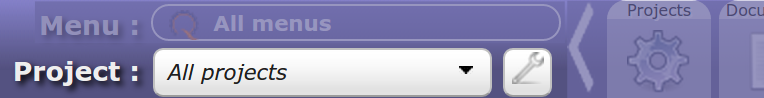
\includegraphics{projectSelector.png}}
\end{figure}
\begin{itemize}
\item {} 
Allows to restrict the visibility of all objects to the dedicated project, including sub-projects if any.

\item {} 
The selection will also define de ``default'' project for new items.

\end{itemize}
\setbox0\vbox{
\begin{minipage}{0.95\linewidth}
\textbf{Project selector parameters}

\medskip


Through the project selector parameter icon \scalebox{0.500000}{\includegraphics{iconParameter32.png}}, you can select :
\begin{itemize}
\item {} 
View closed projects.

\item {} 
Change the project selector format.

\item {} 
Refresh the list.

\end{itemize}
\end{minipage}}
\begin{center}\setlength{\fboxsep}{5pt}\shadowbox{\box0}\end{center}
\begin{figure}[htbp]
\centering

\scalebox{0.600000}{\includegraphics{projectSelectorParameters.png}}
\end{figure}
\newpage
\index{navigation buttons}\paragraph{Navigation buttons}
\begin{figure}[htbp]
\centering

\scalebox{0.600000}{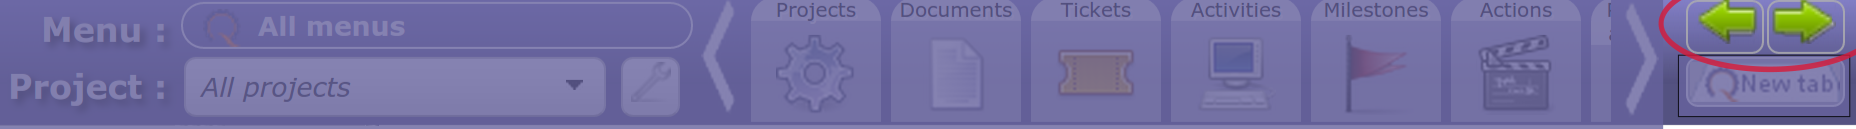
\includegraphics{navigationButtons.png}}
\end{figure}
\begin{itemize}
\item {} 
The navigation buttons \scalebox{0.750000}{\includegraphics{buttonIconBackNavigation.png}} \scalebox{0.750000}{\includegraphics{buttonIconForwardNavigation.png}} give access to previous and next items in the history.

\end{itemize}
\paragraph{New tab button}
\begin{itemize}
\item {} 
Allows to open a new tab with the same session.

\end{itemize}
\begin{figure}[htbp]
\centering

\scalebox{0.600000}{\includegraphics{newTabButton.png}}
\end{figure}
\newpage

\section{Logo area}
\label{Gui:logo-area}\begin{figure}[htbp]
\centering
\capstart

\scalebox{0.600000}{\includegraphics{logoArea.png}}
\caption{Logo area}\end{figure}
\paragraph{Software information}
\begin{itemize}
\item {} 
Clicking on the Logo Area will display the “About” pop-up.

\end{itemize}
\begin{figure}[htbp]
\centering

\scalebox{0.600000}{\includegraphics{softwareInformation.png}}
\end{figure}
\paragraph{Online user manual}
\begin{itemize}
\item {} 
Click on the Help icon \scalebox{0.900000}{\includegraphics{iconHelp.png}} will open the online user manual, to the page corresponding to the actual screen.

\end{itemize}

\begin{notice}{note}{Note:}\begin{itemize}
\item {} 
You can change logo with your own.

\item {} 
Refer to administrative guide to replace the logo.

\end{itemize}
\end{notice}
\newpage

\section{Menu and Documents windows}
\label{Gui:menu-and-documents-windows}\begin{figure}[htbp]
\centering
\capstart

\scalebox{0.600000}{\includegraphics{menuAndDocumentsWindows.png}}
\caption{Menu and Documents windows}\end{figure}

\begin{notice}{note}{Note:}
Toggle windows
\begin{itemize}
\item {} 
You can toggle between Menu and Documents windows.

\item {} 
Just click on window header.

\end{itemize}
\end{notice}
\paragraph{Menu window}

Menu is proposed as a tree view of reachable items.

The presented items will depend on user habilitation to the screens.

Click on a grouping line will expand-shrink the group.

Click on a item will display the corresponding screen in the main area (right side of the screen).
\begin{figure}[htbp]
\centering

\scalebox{0.600000}{\includegraphics{menuWindow.png}}
\end{figure}

\begin{notice}{note}{Note:}
icon size in menu
\begin{itemize}
\item {} 
This parameter defines the size of icons in menu.

\item {} 
See this parameter under ``Display parameters'' section in {\hyperref[UserParameter:user-parameters-label]{\emph{\DUspan{}{User parameters}}}}.

\end{itemize}
\end{notice}
\paragraph{Documents window}
\begin{itemize}
\item {} 
Document directories give direct access to documents contained in the directory.

\end{itemize}
\begin{figure}[htbp]
\centering

\scalebox{0.600000}{\includegraphics{documentsWindow.png}}
\end{figure}
\setbox0\vbox{
\begin{minipage}{0.95\linewidth}
\textbf{Document directories}

\medskip


This icon \scalebox{0.750000}{\includegraphics{iconDocumentDirectory32.png}} gives direct access to the directories management screen.
\end{minipage}}
\begin{center}\setlength{\fboxsep}{5pt}\shadowbox{\box0}\end{center}
\newpage

\section{Message and Link windows}
\label{Gui:message-and-link-windows}\begin{figure}[htbp]
\centering
\capstart

\scalebox{0.600000}{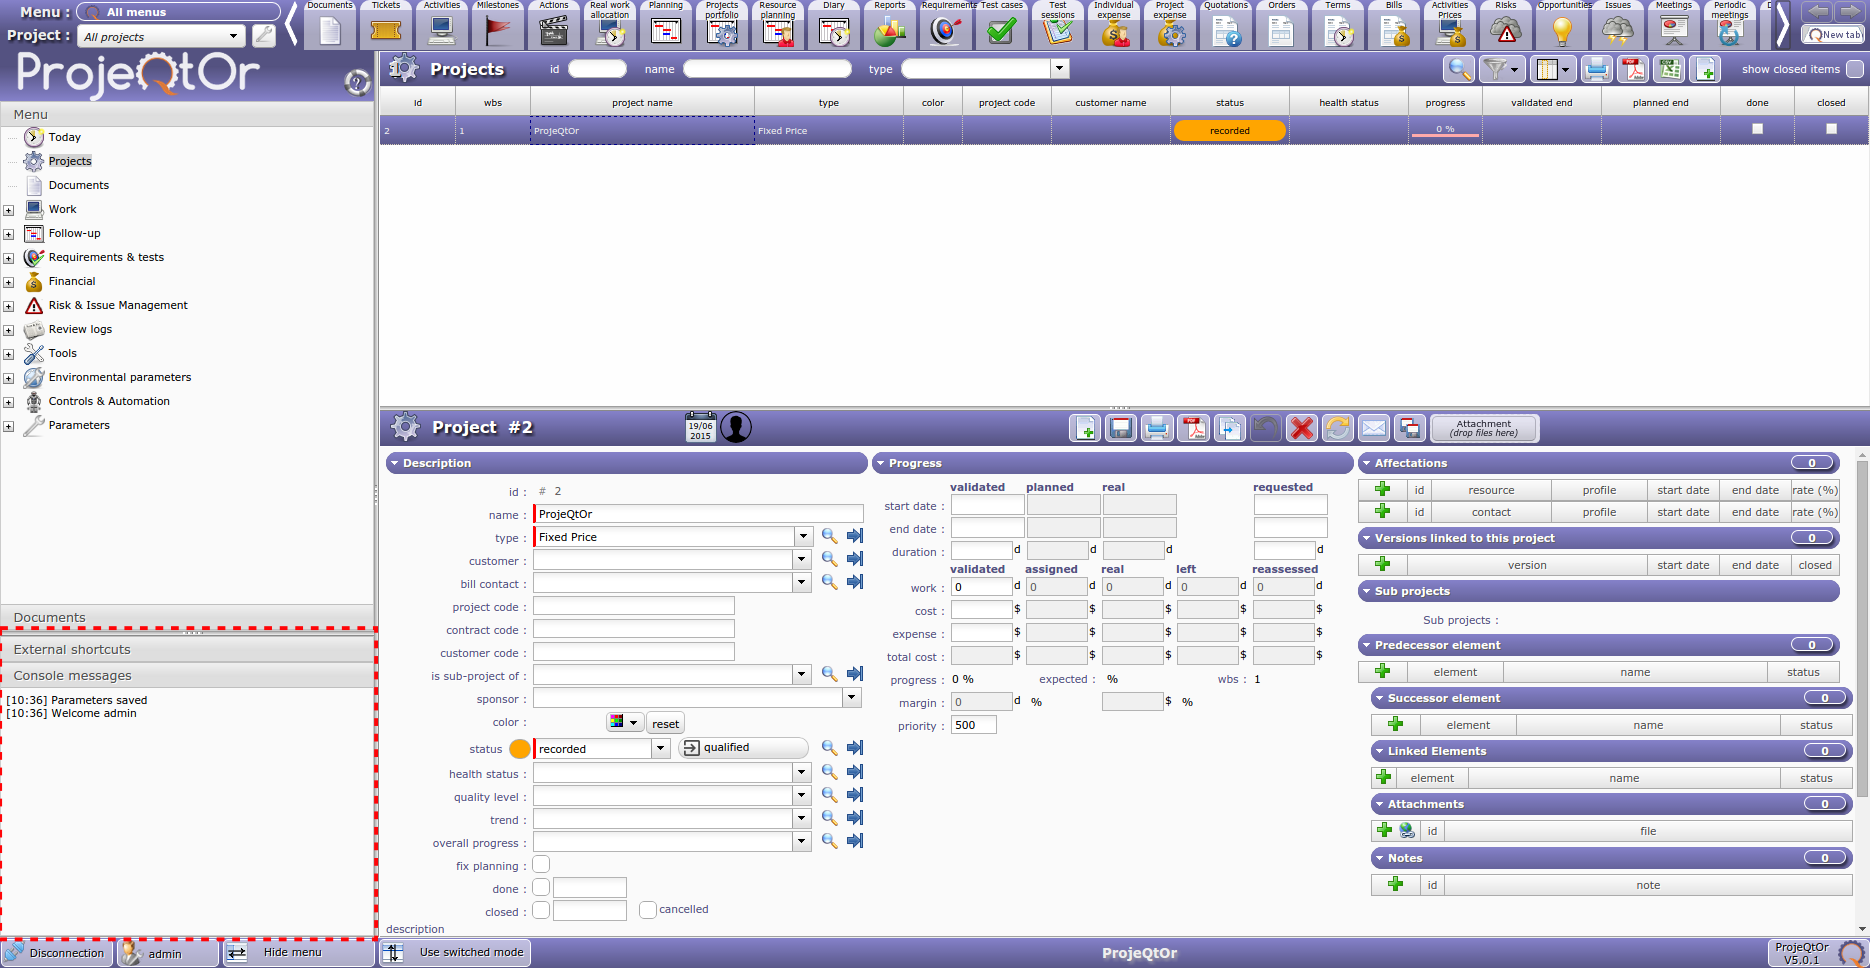
\includegraphics{messageAndLinkWindows.png}}
\caption{Message and Link windows}\end{figure}

\begin{notice}{note}{Note:}
Toggle windows
\begin{itemize}
\item {} 
You can toggle between External shortcuts and Console messages windows.

\item {} 
Just click on window header.

\end{itemize}
\end{notice}
\paragraph{External shortcuts window}
\begin{itemize}
\item {} 
Displays hyperlinks to remote web pages.

\item {} 
Theses links are defined as hyperlink attachements on projects.

\item {} 
Links displayed here depend on selected project.

\end{itemize}
\begin{figure}[htbp]
\centering

\scalebox{0.600000}{\includegraphics{externalShortcuts.png}}
\end{figure}
\paragraph{Console messages window}
\begin{itemize}
\item {} 
Displays information about main actions : insert, update, delete.

\item {} 
Timestamp indicates when action was done.

\end{itemize}
\begin{figure}[htbp]
\centering

\scalebox{0.600000}{\includegraphics{consoleMessages.png}}
\end{figure}

\begin{notice}{note}{Note:}\begin{itemize}
\item {} 
This is only a temporary logging area.

\item {} 
Messages displayed here are not stored and will not live more than user connection.

\end{itemize}
\end{notice}
\newpage

\section{Main area}
\label{Gui:main-area}
The main area (right side of the screen) is generally divided in two parts : List window and Detail window.


\section{List window}
\label{Gui:gui-list-window-label}\label{Gui:list-window}\begin{figure}[htbp]
\centering
\capstart

\scalebox{0.600000}{\includegraphics{listWindow.png}}
\caption{List window}\end{figure}
\begin{figure}[htbp]
\centering

\scalebox{0.600000}{\includegraphics{listWindowPart.png}}
\end{figure}
\paragraph{Element identified}
\begin{itemize}
\item {} 
Identifies the element and the number of listed items is displayed.

\item {} 
Each element are associated to a distinctive icon.

\end{itemize}
\paragraph{Rapid filter}
\begin{itemize}
\item {} 
Rapid filtering fields are proposed : “id”, “name” and “type”.

\item {} 
Any change on “id” and “name” will instantly filter data.
\begin{itemize}
\item {} 
Search is considered as “contains”, so typing “1” in “id” will select “1”, “10”, “11”, “21”, “31” and so on.

\end{itemize}

\item {} 
Selecting a “type” in the combo box will restrict the list to the corresponding type.

\end{itemize}
\newpage\paragraph{Buttons}
\begin{itemize}
\item {} 
Click on the “search button” \scalebox{0.750000}{\includegraphics{buttonIconSearch.png}} to display the textual search area.

\item {} 
Click on the “advanced filter” \scalebox{0.750000}{\includegraphics{iconFilter.png}} to set advanced filter (see : {\hyperref[Gui:gui-advanced-filter-label]{\emph{\DUspan{}{Advanced filter}}}}).

\item {} 
Click on the “select columns to display” \scalebox{0.750000}{\includegraphics{buttonIconColumn.png}} to set columns order (see : {\hyperref[Gui:gui-diplayed-columns-label]{\emph{\DUspan{}{Displayed columns}}}}).

\item {} 
Click on the “print the list” \scalebox{0.750000}{\includegraphics{buttonIconPrint.png}} to get a printable version of the list.

\item {} 
Click on the “export to PDF format” \scalebox{0.750000}{\includegraphics{buttonIconPdf.png}} to export it to PDF format.

\item {} 
Click on the “export to CSV format” \scalebox{0.750000}{\includegraphics{buttonIconCsv.png}} to export all the data of the selected items into CSV format file (see : {\hyperref[Gui:gui-exportcsv-format-label]{\emph{\DUspan{}{Export to CSV format}}}}).

\item {} 
Click on the “create a new \textbf{item}” \scalebox{0.750000}{\includegraphics{buttonIconNew.png}} to create a new item of element.

\end{itemize}
\paragraph{Show closed items flag}
\begin{itemize}
\item {} 
Check the “show closed items” to list also closed items.

\end{itemize}
\paragraph{Columns header}
\begin{itemize}
\item {} 
Click on the header of a column will sort the list on that column (first ascending, then descending).

\end{itemize}

\begin{notice}{note}{Note:}\begin{itemize}
\item {} 
The sorting is not always on the displayed name.
\begin{itemize}
\item {} 
if the sorted column is linked to a reference list with sort order value, the sorting is executed on this sort value
\begin{itemize}
\item {} 
for instance, here the sorting on the status is executed corresponding to Status sort order value, defined as a logic workflow for status change.

\end{itemize}

\end{itemize}

\end{itemize}
\end{notice}
\paragraph{Items list}
\begin{itemize}
\item {} 
Click on a line (any column) will display the corresponding item in the detail window.

\end{itemize}
\newpage

\subsection{Advanced filter}
\label{Gui:advanced-filter}\label{Gui:gui-advanced-filter-label}\begin{figure}[htbp]
\centering

\scalebox{0.600000}{\includegraphics{advancedFilterDefinition.png}}
\end{figure}

The filter pop-up presents two areas : “Active filter” and “Saved filter”.
\paragraph{Active filter}
\begin{itemize}
\item {} 
Enter new clause in Active filter : in “Add a filter or sort clause”, select the name of the field, the operator and the value for the clause.
\begin{itemize}
\item {} 
Then click on \scalebox{0.750000}{\includegraphics{smallButtonAdd.png}} to add the clause to the filter criteria.

\end{itemize}

\item {} 
Click on \scalebox{0.750000}{\includegraphics{smallButtonRemove.png}} on a clause line to remove it.

\item {} 
Click on \scalebox{0.750000}{\includegraphics{smallButtonRemove.png}} on the header of Filter criteria to remove all clauses.
\begin{itemize}
\item {} 
This can also be done by clicking the “Clear” button.

\end{itemize}

\item {} 
When Filter criteria is correct, click on “OK” button to apply the filter to the list.

\item {} 
You can also click “Cancel” button to revert to previous filter.

\item {} 
At any step you can enter a filter name and click on \scalebox{0.750000}{\includegraphics{iconSave.png}} to save the filter definition.

\end{itemize}
\setbox0\vbox{
\begin{minipage}{0.95\linewidth}
\textbf{Operators detail}

\medskip

\begin{itemize}
\item {} 
\textbf{Sort} operator define a sort criteria, then possible values are “ascending” or “descending”.

\item {} 
\textbf{Amongst} operator allows multi-value selection is possible using \code{Control} key.

\end{itemize}
\end{minipage}}
\begin{center}\setlength{\fboxsep}{5pt}\shadowbox{\box0}\end{center}

\begin{notice}{note}{Note:}\begin{itemize}
\item {} 
Filters are defined and stored for a user and a type of item (a screen).

\item {} 
When a filter is applied to a type of item, coming back after moving to another type (another selection in the menu) will apply the previously defined filter.

\item {} 
After disconnection, currently applied filter is lost, but stored filters are saved.
\begin{itemize}
\item {} 
Default filter (if selected) is also stored and will be automatically applied on next connection.

\end{itemize}

\end{itemize}
\end{notice}
\paragraph{Saved filter}
\begin{itemize}
\item {} 
Click on a Saved filter to retrieve its definition (filter criteria).

\item {} 
Click on \scalebox{0.750000}{\includegraphics{smallButtonRemove.png}} on a saved filter to delete it.

\item {} 
Click on “Default” button to set actual stored filter as default, kept even after disconnection.

\end{itemize}

\begin{notice}{note}{Note:}\begin{itemize}
\item {} 
When filter is applied, filter button in the list area is checked \scalebox{0.750000}{\includegraphics{iconActiveFilter.png}}.

\end{itemize}
\end{notice}
\newpage

\subsection{Displayed columns}
\label{Gui:displayed-columns}\label{Gui:gui-diplayed-columns-label}\begin{itemize}
\item {} 
This button opens the list of all available fields.

\item {} 
Just check the fields you want to display in the list.

\item {} 
You can reorder fields with drag \& drop feature, using the selector area \scalebox{0.800000}{\includegraphics{iconDrag.png}}.

\item {} 
When a field is selected, you can change its width with the spinner button.

\end{itemize}
\setbox0\vbox{
\begin{minipage}{0.95\linewidth}
\textbf{Width}

\medskip

\begin{itemize}
\item {} 
Width is in \% of total list width.

\item {} 
Minimum width is 1\%. Maximum width is 50\%.

\item {} 
So, if you select to many columns or set columns width too large, you may have total width over 100\%.
\begin{itemize}
\item {} 
This will be highlighted beside buttons.

\end{itemize}

\item {} 
This may lead to strange display, over page width, on List, reports or pdf export, depending on browser.

\item {} 
It is possible to reset the list display to its default format using the ``reset'' button.

\end{itemize}
\end{minipage}}
\begin{center}\setlength{\fboxsep}{5pt}\shadowbox{\box0}\end{center}

\begin{notice}{note}{Note:}
id and name
\begin{itemize}
\item {} 
“id” and “name” are mandatory fileds : they cannot be removed from display.

\item {} 
The “name” width is automatically adjusted so that total list width is 100\%.

\item {} 
Take care that “name” width cannot be less than 10\%.

\end{itemize}
\end{notice}
\begin{figure}[htbp]
\centering

\scalebox{0.600000}{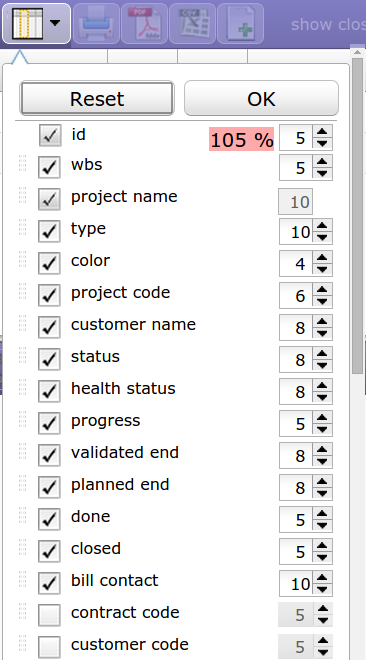
\includegraphics{selectColunmsToDisplay.png}}
\end{figure}
\newpage

\subsection{Export to CSV format}
\label{Gui:export-to-csv-format}\label{Gui:gui-exportcsv-format-label}
The Export pop-up allows to choose fields to export.

The fields are presented in the order as they appear in the item description.
\setbox0\vbox{
\begin{minipage}{0.95\linewidth}
\textbf{Selecting fields}

\medskip

\begin{itemize}
\item {} 
You can easily check or uncheck all fields to export.

\item {} 
You can also easily restrict selected fields to the ones that are actually displayed in the list.

\end{itemize}
\end{minipage}}
\begin{center}\setlength{\fboxsep}{5pt}\shadowbox{\box0}\end{center}
\setbox0\vbox{
\begin{minipage}{0.95\linewidth}
\textbf{id or name for references}

\medskip

\begin{itemize}
\item {} 
For fields that reference another item (displayed as lists in the item description), you can select to export either the id or the clear name of the referenced item.

\end{itemize}
\end{minipage}}
\begin{center}\setlength{\fboxsep}{5pt}\shadowbox{\box0}\end{center}
\begin{figure}[htbp]
\centering

\scalebox{0.600000}{\includegraphics{chooseColumnsToExport.png}}
\end{figure}

\begin{notice}{note}{Note:}\begin{itemize}
\item {} 
CSV exported files can directly be imported through the Import functionality.

\end{itemize}
\end{notice}
\newpage

\section{Detail window}
\label{Gui:detail-window}\begin{figure}[htbp]
\centering
\capstart

\scalebox{0.600000}{\includegraphics{detailWindow.png}}
\caption{Detail window}\end{figure}
\begin{figure}[htbp]
\centering

\scalebox{0.600000}{\includegraphics{detailWindowPart.png}}
\end{figure}
\paragraph{Element identified}
\begin{itemize}
\item {} 
Identifies the element and the item id number.

\item {} 
Each element are associated to a distinctive icon.

\end{itemize}
\paragraph{Creation information}
\begin{itemize}
\item {} 
Information about item creation : issuer and date.

\end{itemize}

\begin{notice}{note}{Note:}\begin{itemize}
\item {} 
Administrator can change information.

\end{itemize}
\end{notice}
\newpage\paragraph{Buttons}
\begin{itemize}
\item {} 
Click on \scalebox{0.750000}{\includegraphics{buttonIconNew.png}} to create new item.

\item {} 
Click on \scalebox{0.750000}{\includegraphics{buttonIconSave.png}} to save the changes.
\begin{itemize}
\item {} 
You can rapidly save with \code{Control-s}.

\end{itemize}

\item {} 
Click on \scalebox{0.750000}{\includegraphics{buttonIconPrint.png}} to get a printable version of the detail.

\item {} 
Click on \scalebox{0.750000}{\includegraphics{buttonIconPdf.png}}  to get a printable version of the detail in PDF format.

\item {} 
Click on \scalebox{0.750000}{\includegraphics{buttonIconCopy.png}} to copy the current item (see : {\hyperref[Gui:gui-copyandtransform-item-label]{\emph{\DUspan{}{Copy item}}}}).

\item {} 
Click on \scalebox{0.750000}{\includegraphics{buttonIconUndo.png}} to cancel ongoing changes.

\item {} 
Click on \scalebox{0.750000}{\includegraphics{buttonIconDelete.png}} to delete the item.

\item {} 
Click on \scalebox{0.750000}{\includegraphics{buttonIconRefresh.png}} to refresh the display.

\item {} 
Click on \scalebox{0.750000}{\includegraphics{buttonIconEmail.png}} to send detail of item by email (see : {\hyperref[Gui:gui-email-detail-label]{\emph{\DUspan{}{Email detail}}}}).

\item {} 
Click on \scalebox{0.750000}{\includegraphics{buttonIconMultipleUpdate.png}} to update several items in one operation (see : {\hyperref[Gui:gui-multiple-update-label]{\emph{\DUspan{}{Multiple update}}}}).

\item {} 
Click on \scalebox{0.750000}{\includegraphics{buttonIconShowChecklist.png}} to show checklist.
\begin{itemize}
\item {} 
Available only when user set user parameter ``display checklists'' to ``On request''.

\item {} 
For detail of checklist information, see {\hyperref[Gui:gui-checklist-section-label]{\emph{\DUspan{}{Section: Checklist}}}}.

\end{itemize}

\item {} 
Click on \scalebox{0.750000}{\includegraphics{buttonIconShowHistory.png}} to show history of changes.
\begin{itemize}
\item {} 
Available only when user set user parameter ``display history'' to ``On request''.

\item {} 
For detail of history of changes information, see {\hyperref[Gui:gui-chg-history-section-label]{\emph{\DUspan{}{Section: Change history}}}}.

\end{itemize}

\end{itemize}

\begin{notice}{note}{Note:}\begin{itemize}
\item {} 
Some buttons are not clickable when change are ongoing.

\item {} 
\scalebox{0.750000}{\includegraphics{buttonIconUndo.png}} button is clickable only when changes are ongoing.

\end{itemize}
\end{notice}

\begin{notice}{warning}{Warning:}\begin{itemize}
\item {} 
When changes are ongoing, you can not select another item or another menu item.

\item {} 
Save or cancel ongoing changes first.

\end{itemize}
\end{notice}
\paragraph{Drop file area}
\begin{itemize}
\item {} 
This area allows to add a attachement file in item.
\begin{itemize}
\item {} 
You can drag and drop file.

\item {} 
Or click on area to select file.

\end{itemize}

\end{itemize}
\paragraph{Sections}
\begin{itemize}
\item {} 
The fields are regrouped under section.

\item {} 
All sections can be folded or unfolded, clicking on the section title.

\item {} 
The sections are organized in columns.
\begin{itemize}
\item {} 
Maximum three columns can be displayed.

\end{itemize}

\item {} 
Some sections are displayed on almost all screens, see : {\hyperref[Gui:gui-sections-label]{\emph{\DUspan{}{Common sections}}}}

\end{itemize}
\newpage

\subsection{Copy item}
\label{Gui:copy-item}\label{Gui:gui-copyandtransform-item-label}\begin{itemize}
\item {} 
Allows copied item of element.

\item {} 
Options displayed in pop-up depends on whether an item is simple or complex.

\end{itemize}
\begin{figure}[htbp]
\centering

\scalebox{0.600000}{\includegraphics{copyElement.png}}
\end{figure}
\setbox0\vbox{
\begin{minipage}{0.95\linewidth}
\textbf{Simple items}

\medskip

\begin{itemize}
\item {} 
Simple items (environment parameters, lists, …) can only be copied “as is”.

\end{itemize}
\end{minipage}}
\begin{center}\setlength{\fboxsep}{5pt}\shadowbox{\box0}\end{center}
\setbox0\vbox{
\begin{minipage}{0.95\linewidth}
\textbf{Complex items}

\medskip

\begin{itemize}
\item {} 
Complex items (Tickets, Activities, …) it is possible to copy them into new kind of elements.

\item {} 
For instance, it is possible to copy a Ticket (the request) into an Activity (the task to manage the request).

\item {} 
It is possible to select :
\begin{itemize}
\item {} 
New kind of element.

\item {} 
Select new type (corresponding to the kind of element).

\item {} 
Change the name.

\item {} 
Select whether the initial element will be indicated as origin of the copied one.

\item {} 
For main items, it is also possible to choose to copy links, attachments and notes.

\end{itemize}

\begin{notice}{note}{Note:}\begin{itemize}
\item {} 
For Projects and Activities, it is also possible to copy the hierarchic structure of activities (sub-projects, sub-activities).

\item {} 
The new item are the status ``copied''.

\end{itemize}
\end{notice}

\end{itemize}
\end{minipage}}
\begin{center}\setlength{\fboxsep}{5pt}\shadowbox{\box0}\end{center}


\subsection{Email detail}
\label{Gui:gui-email-detail-label}\label{Gui:email-detail}
It is possible to send an informative email to defined recipients list.

\textbf{message}
\begin{itemize}
\item {} 
The message that will be included in the body of the email, in addition to complete description of item.

\end{itemize}
\newpage

\subsection{Multiple update}
\label{Gui:multiple-update}\label{Gui:gui-multiple-update-label}
To update several items in one operation.

This will switch to new detail view :
\begin{figure}[htbp]
\centering

\scalebox{0.600000}{\includegraphics{multipleModePart1.png}}
\end{figure}

At this step, although the list does not seem to have changed, but it is now multi-selectable :
\begin{figure}[htbp]
\centering

\scalebox{0.600000}{\includegraphics{multipleModePart2.png}}
\end{figure}

Select lines of items you want to update, specify update and save : the update will be applied to all the items (if possible) and a report will be displayed on the right of the Multiple mode detail screen.
\begin{figure}[htbp]
\centering

\scalebox{0.600000}{\includegraphics{multipleModePart3.png}}
\end{figure}
\newpage

\subsection{Combo list fields}
\label{Gui:combo-list-fields}\label{Gui:gui-combo-list-fields-label}
Combo list field allows to search, view or create item associate with the field.
\begin{figure}[htbp]
\centering
\capstart

\scalebox{0.600000}{\includegraphics{comboListFields.png}}
\caption{Example}\end{figure}
\begin{itemize}
\item {} 
Click on \scalebox{0.750000}{\includegraphics{comboArrowDown.png}} to get the list of value.

\item {} 
Click on \scalebox{0.750000}{\includegraphics{buttonIconSearch.png}} to access item details.
\begin{itemize}
\item {} 
The action depends on whether the element is selected or not.

\end{itemize}

\item {} 
Click on \scalebox{0.750000}{\includegraphics{iconGoto.png}} will directly go to the selected item.

\end{itemize}

\begin{notice}{note}{Note:}\begin{itemize}
\item {} 
Access to view or create item depends on your access rights.

\item {} 
Some buttons become not available.

\end{itemize}
\end{notice}
\paragraph{Element is selected}

If element is selected in the combo, detail of element is displayed.
\begin{figure}[htbp]
\centering

\scalebox{0.600000}{\includegraphics{detailOfListElementOpt1.png}}
\end{figure}
\begin{itemize}
\item {} 
Click on \scalebox{0.750000}{\includegraphics{buttonIconSearch.png}} to search an item.

\item {} 
Click on \scalebox{0.750000}{\includegraphics{buttonIconUndo.png}} to close the window.

\end{itemize}
\newpage\paragraph{No element is selected}

If no element is selected, list of elements is displayed, allowing to select an item.
\begin{figure}[htbp]
\centering

\scalebox{0.600000}{\includegraphics{detailOfListElementOpt2.png}}
\end{figure}
\begin{itemize}
\item {} 
Click on \scalebox{0.750000}{\includegraphics{buttonIconSelect.png}} to select item.

\item {} 
Click on \scalebox{0.750000}{\includegraphics{buttonIconNew.png}} to create a new item.

\item {} 
Click on \scalebox{0.750000}{\includegraphics{buttonIconUndo.png}} to close the window.

\end{itemize}

\begin{notice}{note}{Note:}
Header window
\begin{itemize}
\item {} 
You have access to rapid filter, search button and advanced filter.

\item {} 
For detail, see : {\hyperref[Gui:gui-list-window-label]{\emph{\DUspan{}{List window}}}}.

\end{itemize}
\end{notice}

\begin{notice}{note}{Note:}
Select several items
\begin{itemize}
\item {} 
Some elements is possible to select several items, use \code{Control} or \code{Shift}.

\end{itemize}
\end{notice}
\paragraph{Go to selected item}
\begin{itemize}
\item {} 
Click on \scalebox{0.750000}{\includegraphics{iconGoto.png}} will directly go to the selected item.

\end{itemize}

\begin{notice}{note}{Note:}
Return to last screen
\begin{itemize}
\item {} 
Click on \scalebox{0.750000}{\includegraphics{buttonIconBackNavigation.png}} to return on last screen.

\item {} 
For detail, see \textbf{Navigation buttons} in {\hyperref[Gui:gui-top-bar-label]{\emph{\DUspan{}{Top bar}}}} section.

\end{itemize}
\end{notice}
\newpage

\subsection{Long text fields}
\label{Gui:long-text-fields}\begin{figure}[htbp]
\centering
\capstart

\scalebox{0.600000}{\includegraphics{longTextFields.png}}
\caption{Example}\end{figure}
\begin{itemize}
\item {} 
Long text fields allow to write description, results, notes, ...

\item {} 
A mini editor is provided.

\item {} 
Text zone is expendable.

\end{itemize}

\begin{notice}{note}{Note:}
Editor mode always on
\begin{itemize}
\item {} 
This parameter defines editor is always on in long text fields.

\item {} 
See this parameter under ``Graphic interface behavior'' section in {\hyperref[UserParameter:user-parameters-label]{\emph{\DUspan{}{User parameters}}}}.

\end{itemize}
\end{notice}
\newpage

\section{Info bar}
\label{Gui:info-bar}\begin{figure}[htbp]
\centering
\capstart

\scalebox{0.600000}{\includegraphics{infobar.png}}
\caption{Info bar}\end{figure}
\begin{figure}[htbp]
\centering

\scalebox{0.600000}{\includegraphics{infobarPart.png}}
\end{figure}
\paragraph{Log out button}
\begin{itemize}
\item {} 
Allow to disconnect user.

\end{itemize}

\begin{notice}{note}{Note:}
confirm quit application
\begin{itemize}
\item {} 
This parameter defines whether a confirm disconnection will be displayed before.

\item {} 
See this parameter under ``Graphic interface behavior'' section in {\hyperref[UserParameter:user-parameters-label]{\emph{\DUspan{}{User parameters}}}}.

\end{itemize}
\end{notice}
\paragraph{User parameters button}
\begin{itemize}
\item {} 
Allow to access user parameters.

\end{itemize}
\paragraph{Hide and show menu button}
\begin{itemize}
\item {} 
Allow to hide or show menu button

\end{itemize}

\begin{notice}{note}{Note:}
hide menu
\begin{itemize}
\item {} 
This parameter defines whether the menu is hidden by default.

\item {} 
See this parameter under ``Graphic interface behavior'' section in {\hyperref[UserParameter:user-parameters-label]{\emph{\DUspan{}{User parameters}}}}.

\end{itemize}
\end{notice}
\paragraph{Switched mode button}
\begin{itemize}
\item {} 
Allow to enable or disable switched mode between list and detail windows.

\item {} 
Window selected is displayed in ``full screen'' mode.

\item {} 
Hidden window are replaced by a gray bar.

\item {} 
Click on he gray bar to switch between windows.

\end{itemize}

\begin{notice}{note}{Note:}
switched mode
\begin{itemize}
\item {} 
This parameter defines wheater switched mode is enable or not.

\item {} 
See this parameter under ``Graphic interface behavior'' section in {\hyperref[UserParameter:user-parameters-label]{\emph{\DUspan{}{User parameters}}}}.

\end{itemize}
\end{notice}
\paragraph{Database name}
\begin{itemize}
\item {} 
Display database name.

\end{itemize}
\paragraph{Version button}
\begin{itemize}
\item {} 
Display application version.

\item {} 
Click on button access to ProjeQtOr site.

\end{itemize}
\newpage

\section{Common sections}
\label{Gui:gui-sections-label}\label{Gui:common-sections}
Some sections are displayed on almost all screens.

Those sections allows to set information or link information to item of the element.


\subsection{Section: Description}
\label{Gui:section-description}
This section allows to put information about item of the element.


\subsection{Section: Treatment}
\label{Gui:section-treatment}
This section allows to put information treatment done on the item of the element.

Mostly information under this section are :
\begin{itemize}
\item {} 
Status and Dates

\item {} 
Responsible

\item {} 
Result, Comment

\item {} 
And so on

\end{itemize}


\subsection{Section: Checklist}
\label{Gui:gui-checklist-section-label}\label{Gui:section-checklist}
If a checklist is defined for the current element a checklist section will appear.

The user just has to check information corresponding to the situation.

When done, the user name and checked date are recorded and displayed.

Each line can get an extra comment, as well a globally on the checklist.

\begin{notice}{note}{Note:}\begin{itemize}
\item {} 
How to define a checklist, see: {\hyperref[ControlAutomation:ctrlauto-checklist-def-label]{\emph{\DUspan{}{Checklist definition}}}}.

\end{itemize}
\end{notice}

\begin{notice}{note}{Note:}
display checklists
\begin{itemize}
\item {} 
This parameter defines whether the checklist section is hidden or not.

\item {} 
If the value ``On request'' is set \scalebox{0.750000}{\includegraphics{buttonIconShowChecklist.png}} button appear on detail header window.

\item {} 
See this parameter under ``Graphic interface behavior'' section in {\hyperref[UserParameter:user-parameters-label]{\emph{\DUspan{}{User parameters}}}}.

\end{itemize}
\end{notice}
\newpage

\subsection{Section: Linked element}
\label{Gui:section-linked-element}\label{Gui:gui-linkelement-section-label}
Most items can be linked to most of all other items (Actions, Activities, Tickets, Documents, …).

\begin{notice}{note}{Note:}
Linked elements must belong to the same project.
\end{notice}

Click \scalebox{0.750000}{\includegraphics{smallButtonAdd.png}} on the corresponding section to add a link to an element. A “add link” pop up will be displayed.

Select the linked element in the list and validate (OK).

Click on \scalebox{0.750000}{\includegraphics{smallButtonRemove.png}} to delete the corresponding link.
\begin{figure}[htbp]
\centering
\capstart

\scalebox{0.600000}{\includegraphics{addLink.png}}
\caption{Add link Popup}\end{figure}
\setbox0\vbox{
\begin{minipage}{0.95\linewidth}
\textbf{Linked element}

\medskip

\begin{itemize}
\item {} 
Click on \scalebox{0.750000}{\includegraphics{buttonIconSearch.png}} to show element detail.

\item {} 
Depends on whether the element is selected or not a pop up is displayed.

\item {} 
Detail about pop up, see {\hyperref[Gui:gui-combo-list-fields-label]{\emph{\DUspan{}{Combo list fields}}}}

\end{itemize}
\end{minipage}}
\begin{center}\setlength{\fboxsep}{5pt}\shadowbox{\box0}\end{center}
\paragraph{Linked elements information}

\begin{tabulary}{\linewidth}{|l|l|}
\hline
\textsf{\relax 
Field
} & \textsf{\relax 
Description
}\\
\hline
Element
 & 
Type and id of the linked element.
\\
\hline
Name
 & 
Name of the linked element.
\\
\hline
Date
 & 
Date of creation of the link.
\\
\hline
User
 & 
User who created the link.
\\
\hline
Status
 & 
Actual status of the linked element.
\\
\hline\end{tabulary}

\setbox0\vbox{
\begin{minipage}{0.95\linewidth}
\textbf{Reciprocally interrelated}

\medskip

\begin{itemize}
\item {} 
If Item A is linked to Item B, Item B is automatically linked to Item A.

\end{itemize}
\end{minipage}}
\begin{center}\setlength{\fboxsep}{5pt}\shadowbox{\box0}\end{center}
\setbox0\vbox{
\begin{minipage}{0.95\linewidth}
\textbf{Go to}

\medskip

\begin{itemize}
\item {} 
Click on the name of a item in the link list will directly move to it.

\end{itemize}
\end{minipage}}
\begin{center}\setlength{\fboxsep}{5pt}\shadowbox{\box0}\end{center}
\setbox0\vbox{
\begin{minipage}{0.95\linewidth}
\textbf{Link with Document}

\medskip

\begin{itemize}
\item {} 
If you select a Document to link, you’ll have the possibility to select a version of the document, so that it is the version that will be linked.

\item {} 
For Documents and Document Versions, a direct link to the corresponding file is proposed.

\item {} 
For document, the last version of document will be proposed, the proposed download will change with document lifecycle.

\end{itemize}

\index{attachment - section|textbf}\end{minipage}}
\begin{center}\setlength{\fboxsep}{5pt}\shadowbox{\box0}\end{center}


\subsection{Section: Attachments}
\label{Gui:index-4}\label{Gui:gui-attachment-section-label}\label{Gui:section-attachments}
Users can attach files or hyperlinks on most of items.

Click on \scalebox{0.750000}{\includegraphics{smallButtonAdd.png}} to add a attachment to an element. A “Attachment file” pop up will be displayed.

Click on \scalebox{0.750000}{\includegraphics{smallButtonLink.png}} to add hyperlink to an element. A “Attachment hyperlink” pop up will be displayed.

Select the attachment depends on either is a file or a hyperlink and validate (OK).

Click on \scalebox{0.750000}{\includegraphics{smallButtonDownload.png}} to download attachment file.

Click on \scalebox{0.750000}{\includegraphics{smallButtonLink.png}} to access to hyperlink.

Click on \scalebox{0.750000}{\includegraphics{smallButtonRemove.png}} to delete the attachment.
\paragraph{Attachment file}
\begin{itemize}
\item {} 
To upload file :
\begin{itemize}
\item {} 
Select file with ``Browse'' button.

\item {} 
Drop the file in ``drop files here'' area.

\end{itemize}

\end{itemize}
\begin{figure}[htbp]
\centering
\capstart

\scalebox{0.600000}{\includegraphics{attachmentFile.png}}
\caption{Attachment file Pop up}\end{figure}
\paragraph{Hyperlink}
\begin{itemize}
\item {} 
Set hyperlink in hyperlink field.

\end{itemize}
\begin{figure}[htbp]
\centering
\capstart

\scalebox{0.600000}{\includegraphics{attachmentHyperLink.png}}
\caption{Attachment hyperlink Pop up}\end{figure}
\paragraph{Attachment visibilty}
\begin{itemize}
\item {} 
public : Visible to anyone.

\item {} 
team : Visible to every member of the creator’s team.

\item {} 
private :  Visible only to creator.

\end{itemize}
\paragraph{Attachment information}

\begin{tabulary}{\linewidth}{|l|l|}
\hline
\textsf{\relax 
Field
} & \textsf{\relax 
Description
}\\
\hline
{\hyperref[Glossary:term-id]{\emph{\DUspan{xref,std,std-term}{Id}}}}
 & 
Unique Id for the attachment.
\\
\hline
File
 & 
File name or hyperlink.
\\
\hline
Date
 & 
Date of creation of the attachment.
\\
\hline
User
 & 
User who created the attchment.
\\
\hline\end{tabulary}


\index{note - section|textbf}

\subsection{Section: Notes}
\label{Gui:index-5}\label{Gui:gui-note-section-label}\label{Gui:section-notes}
Users can add notes on most items.

Notes are comments, that can be shared to track some information or progress.

Click on \scalebox{0.750000}{\includegraphics{smallButtonAdd.png}} to add a note to an element. A “note” pop up will be displayed.

Click on \scalebox{0.750000}{\includegraphics{smallButtonEdit.png}} to edit the note.

Click on \scalebox{0.750000}{\includegraphics{smallButtonRemove.png}} to delete the note.
\begin{figure}[htbp]
\centering
\capstart

\scalebox{0.600000}{\includegraphics{note1.png}}
\caption{Note Pop up}\end{figure}
\paragraph{Predefined note}
\begin{itemize}
\item {} 
Predefined note list of value appear whetear a prefedefined note is created.

\item {} 
Selecting an item in the list will automatically fill in the note text field.

\item {} 
How to define predefined note, see: {\hyperref[ControlAutomation:ctrlauto-predefined-notes-label]{\emph{\DUspan{}{Predefined notes}}}}.

\end{itemize}
\paragraph{Attachment visibilty}
\begin{itemize}
\item {} 
public : Visible to anyone.

\item {} 
team : Visible to every member of the creator’s team.

\item {} 
private :  Visible only to creator.

\end{itemize}
\paragraph{Note information}

\begin{tabulary}{\linewidth}{|l|l|}
\hline
\textsf{\relax 
Field
} & \textsf{\relax 
Description
}\\
\hline
{\hyperref[Glossary:term-id]{\emph{\DUspan{xref,std,std-term}{Id}}}}
 & 
Unique Id for the note.
\\
\hline
Note
 & 
Text of the note.
\\
\hline
Date
 & 
Date of creation or modification of the note.
\\
\hline
User
 & 
Name of the user who created the note.
\\
\hline\end{tabulary}


\index{history - section|textbf}

\subsection{Section: Change history}
\label{Gui:section-change-history}\label{Gui:gui-chg-history-section-label}\label{Gui:index-6}
All the changes items are tracked.

They are stored and displayed on each item.

On creation, just an insert operation is stored, not all the initial values on creation.
\paragraph{Change history information}

\begin{tabulary}{\linewidth}{|l|l|}
\hline
\textsf{\relax 
Field
} & \textsf{\relax 
Description
}\\
\hline
Operation
 & 
The operation on the item (insert or update).
\\
\hline
Data
 & 
The field modified.
\\
\hline
Value before
 & 
The value of the field before the update.
\\
\hline
Value after
 & 
The value of the field after the update.
\\
\hline
Date
 & 
Date of change operation.
\\
\hline
User
 & 
Name of the user who operated the change.
\\
\hline\end{tabulary}


\begin{notice}{note}{Note:}
display history
\begin{itemize}
\item {} 
This parameter defines whether the display history section is hidden or not.

\item {} 
If the value ``On request'' is set \scalebox{0.750000}{\includegraphics{buttonIconShowHistory.png}} button appear on the detail header window.

\item {} 
See this parameter under ``Graphic interface behavior'' section in {\hyperref[UserParameter:user-parameters-label]{\emph{\DUspan{}{User parameters}}}}.

\end{itemize}
\end{notice}
\newpage

\section{Alerts}
\label{Gui:alerts}
You may receive some information displayed as pop-up on the bottom right corner of the screen.

Three kinds of information may be displayed :
\begin{itemize}
\item {} 
Information

\item {} 
Warning

\item {} 
Alert

\end{itemize}

Two possible actions :
\begin{itemize}
\item {} 
You can select to remind you in a given number of minutes (message will close and appear  again in the given number of minutes).

\item {} 
You can mark it as read to definitively hide it.

\end{itemize}

An alert can be sent by the administrator or indicator calculation.

\begin{notice}{note}{Note:}
Administrator
\begin{itemize}
\item {} 
Administrator can send alert by administration console.

\end{itemize}
\end{notice}

\begin{notice}{note}{Note:}
Indicator calculation
\begin{itemize}
\item {} 
Indicator calculation send only warning and alert message.

\item {} 
Alert coming from indicator calculation message contains more information :
\begin{itemize}
\item {} 
Item id and type.

\item {} 
Indicator description.

\item {} 
Target value.

\item {} 
Alert or warning value.

\end{itemize}

\end{itemize}
\end{notice}
\newpage

\section{Themes}
\label{Gui:themes}
Users can select colors Theme to display the interface.

New theme is automatically applied when selected.

\begin{notice}{note}{Note:}
theme
\begin{itemize}
\item {} 
This parameter defines the theme to display.

\item {} 
Save parameters to retrieve this theme on each new connection.

\item {} 
See this parameter under ``Display parameters'' section in {\hyperref[UserParameter:user-parameters-label]{\emph{\DUspan{}{User parameters}}}}.

\end{itemize}
\end{notice}
\newpage

\section{Multilingual}
\label{Gui:multilingual}
ProjeQtOr is multilingual.

Each user can choose the language to display all the captions.

\begin{notice}{note}{Note:}
Of course, data is displayed as input, no translation is operated.
\end{notice}

\begin{notice}{note}{Note:}
language
\begin{itemize}
\item {} 
This parameter defines language is used to display captions.

\item {} 
Save parameters to retrieve this theme on each new connection.

\item {} 
See this parameter under ``Display parameters'' section in {\hyperref[UserParameter:user-parameters-label]{\emph{\DUspan{}{User parameters}}}}.

\end{itemize}
\end{notice}
\newpage
\index{User parameters|textbf}

\section{User parameters}
\label{UserParameter:user-parameters}\label{UserParameter:user-parameters-label}\label{UserParameter:index-0}\label{UserParameter::doc}
User parameters screen allows configuration of personal settings.
\paragraph{Display parameters}
\begin{itemize}
\item {} 
Generic display parameter for user.

\end{itemize}
\paragraph{Graphic interface behavior}
\begin{itemize}
\item {} 
Selection of graphic interface behavior.

\end{itemize}
\paragraph{Print and Export parameters}
\begin{itemize}
\item {} 
Selection of printing history for detailed items and destination for printing and PDF export.

\end{itemize}
\paragraph{Miscellaneous}
\begin{itemize}
\item {} 
Default selected project and choice of character used to indent lists of projects, to represent the WBS structure of projects and sub-project (cannot be a “space”, can be “none” to get flat lists).

\end{itemize}
\paragraph{Photo}
\begin{itemize}
\item {} 
Add a picture for the user.

\end{itemize}
\paragraph{Password}
\begin{itemize}
\item {} 
Changes the user's password.

\end{itemize}

\begin{notice}{note}{Note:}\begin{itemize}
\item {} 
User parameters are efficient even without saving.

\item {} 
Saving parameters will retrieve the selected parameters on each connection.

\end{itemize}
\end{notice}


\chapter{Planning elements}
\label{index:planning-elements}
ProjeQtOr provides all the elements needed to build a planning from workload,
constraints between tasks and resources availability.
\newpage\setbox0\vbox{
\begin{minipage}{0.95\linewidth}
\textbf{Planning elements}

\medskip

\begin{itemize}
\item {} 
\phantomsection\label{PlanningElements:id8}{\hyperref[PlanningElements:project]{\emph{Project}}}

\item {} 
\phantomsection\label{PlanningElements:id9}{\hyperref[PlanningElements:activity]{\emph{Activity}}}

\item {} 
\phantomsection\label{PlanningElements:id10}{\hyperref[PlanningElements:milestone]{\emph{Milestone}}}

\item {} 
\phantomsection\label{PlanningElements:id11}{\hyperref[PlanningElements:common-sections]{\emph{Common sections}}}
\begin{itemize}
\item {} 
\phantomsection\label{PlanningElements:id12}{\hyperref[PlanningElements:section-affectations]{\emph{Section: Affectations}}}

\item {} 
\phantomsection\label{PlanningElements:id13}{\hyperref[PlanningElements:section-assignment]{\emph{Section: Assignment}}}

\item {} 
\phantomsection\label{PlanningElements:id14}{\hyperref[PlanningElements:section-progress]{\emph{Section: Progress}}}

\item {} 
\phantomsection\label{PlanningElements:id15}{\hyperref[PlanningElements:sections-predecessor-and-sucessor-element]{\emph{Sections: Predecessor and Sucessor element}}}

\end{itemize}

\end{itemize}
\end{minipage}}
\begin{center}\setlength{\fboxsep}{5pt}\shadowbox{\box0}\end{center}

Planning elements are : {\hyperref[PlanningElements:pe-project-label]{\emph{\DUspan{}{Project}}}}, {\hyperref[PlanningElements:pe-activity-label]{\emph{\DUspan{}{Activity}}}}, {\hyperref[PlanningElements:pe-milestone-label]{\emph{\DUspan{}{Milestone}}}}, {\hyperref[RequirementsTest:reqtest-test-session-label]{\emph{\DUspan{}{Test session}}}}, {\hyperref[ReviewLogs:reviewlogs-meeting-label]{\emph{\DUspan{}{Meeting}}}} and {\hyperref[ReviewLogs:reviewlogs-periodic-meeting-label]{\emph{\DUspan{}{Periodic Meeting}}}}.

All previous elements can be planning, following with Gantt chart.
\setbox0\vbox{
\begin{minipage}{0.95\linewidth}
\textbf{Progress}

\medskip

\begin{itemize}
\item {} 
All planning elements have own progress data.

\item {} 
Some metrics are consolidate on top activities and project.

\end{itemize}
\end{minipage}}
\begin{center}\setlength{\fboxsep}{5pt}\shadowbox{\box0}\end{center}
\newpage
\index{project|textbf}

\section{Project}
\label{PlanningElements:project}\label{PlanningElements:pe-project-label}\label{PlanningElements:index-0}\label{PlanningElements::doc}\setbox0\vbox{
\begin{minipage}{0.95\linewidth}
\textbf{Other sections}

\medskip

\begin{itemize}
\item {} 
{\hyperref[PlanningElements:pe-progress-section-label]{\emph{\DUspan{}{Section: Progress}}}}

\item {} 
{\hyperref[PlanningElements:pe-affectations-section-label]{\emph{\DUspan{}{Section: Affectations}}}}

\item {} 
{\hyperref[PlanningElements:pe-predsuces-element-section-label]{\emph{\DUspan{}{Sections: Predecessor and Sucessor element}}}}

\item {} 
{\hyperref[Gui:gui-linkelement-section-label]{\emph{\DUspan{}{Section: Linked element}}}}

\item {} 
{\hyperref[Gui:gui-attachment-section-label]{\emph{\DUspan{}{Section: Attachments}}}}

\item {} 
{\hyperref[Gui:gui-note-section-label]{\emph{\DUspan{}{Section: Notes}}}}

\item {} 
{\hyperref[Gui:gui-chg-history-section-label]{\emph{\DUspan{}{Section: Change history}}}}

\end{itemize}
\end{minipage}}
\begin{center}\setlength{\fboxsep}{5pt}\shadowbox{\box0}\end{center}
\paragraph{Section: Description}

\begin{tabulary}{\linewidth}{|l|l|}
\hline
\textsf{\relax 
Field
} & \textsf{\relax 
Description
}\\
\hline
{\hyperref[Glossary:term-id]{\emph{\DUspan{xref,std,std-term}{Id}}}}
 & 
Unique Id for the project.
\\
\hline
\textbf{Name}
 & 
Short name of the project.
\\
\hline
\textbf{Type}
 & 
Type of project.
\\
\hline
Customer
 & 
The customer of the project.
\\
\hline
Bill contact
 & 
Billing contact.
\\
\hline
Project code
 & 
Code of the project.
\\
\hline
Contract code
 & 
Code of the contract of the project.
\\
\hline
Customer code
 & 
Code of the customer of the project.
\\
\hline
Is sub-project of
 & 
Name of the top project if this project is a sub-project.
\\
\hline
Sponsor
 & 
Name of the sponsor of the project.
\\
\hline
Manager
 & 
Name of the resource who manages the project (Project Leader).
\\
\hline
Color
 & 
Color of the project, to be displayed in some reports.
\\
\hline
\textbf{Status}
 & 
Actual {\hyperref[Glossary:term-status]{\emph{\DUspan{xref,std,std-term}{status}}}} of the project.
\\
\hline
Health status
 & 
Global health status of the project, displayed on today screen.
\\
\hline
Quality level
 & 
Estimation of quality level of project (result of audits).
\\
\hline
Trend
 & 
Trend of global project health.
\\
\hline
Overall progress
 & 
Overall progress to be selected in a defined list.
\\
\hline
Fix planning
 & 
Selector to fix the planning of the project, and its sub-projects.
\\
\hline
{\hyperref[Glossary:term-done]{\emph{\DUspan{xref,std,std-term}{Done}}}}
 & 
Flag to indicate that project is been finished.
\\
\hline
{\hyperref[Glossary:term-closed]{\emph{\DUspan{xref,std,std-term}{Closed}}}}
 & 
Flag to indicate that project is archived.
\\
\hline
Cancelled
 & 
Flag to indicate that project is cancelled.
\\
\hline
Description
 & 
Complete description of the project.
\\
\hline
Objectives
 & 
Objectives of the project.
\\
\hline\end{tabulary}


\textbf{* Required field}
\paragraph{Section: Version linked to this project}
\paragraph{Section: Sub projects}
\newpage
\index{activity|textbf}

\section{Activity}
\label{PlanningElements:pe-activity-label}\label{PlanningElements:index-1}\label{PlanningElements:activity}
An activity is a kind of task that must be planned, or that regroups other activities.

It is generally a long time activity, that will be assigned to one or more resources.

Activities will appear on Gantt planning view.

For instance, you can manage as activities :
\begin{itemize}
\item {} 
Planned tasks.

\item {} 
Change requests.

\item {} 
Phases.

\item {} 
Versions or releases.

\end{itemize}
\paragraph{Activities regroupment}
\begin{itemize}
\item {} 
Activities can have parents to regroup activities.

\item {} 
So a WBS (work breakdown structure number) is calculated for the activities.

\item {} 
Activities can be sorted inside their parent activity, on the Gantt planning view, using drag and drop.

\item {} 
Parent activity must belong to the same project.

\end{itemize}
\paragraph{Assigned ressources}
\begin{itemize}
\item {} 
Resources are can be assigned to activities.

\item {} 
This means that some work is planned on this activity for the resources.

\item {} 
See : {\hyperref[PlanningElements:pe-assignment-section-label]{\emph{\DUspan{}{Section: Assignment}}}}

\end{itemize}
\setbox0\vbox{
\begin{minipage}{0.95\linewidth}
\textbf{Other sections}

\medskip

\begin{itemize}
\item {} 
{\hyperref[PlanningElements:pe-assignment-section-label]{\emph{\DUspan{}{Section: Assignment}}}}

\item {} 
{\hyperref[PlanningElements:pe-progress-section-label]{\emph{\DUspan{}{Section: Progress}}}}

\item {} 
{\hyperref[PlanningElements:pe-predsuces-element-section-label]{\emph{\DUspan{}{Sections: Predecessor and Sucessor element}}}}

\item {} 
{\hyperref[Gui:gui-linkelement-section-label]{\emph{\DUspan{}{Section: Linked element}}}}

\item {} 
{\hyperref[Gui:gui-attachment-section-label]{\emph{\DUspan{}{Section: Attachments}}}}

\item {} 
{\hyperref[Gui:gui-note-section-label]{\emph{\DUspan{}{Section: Notes}}}}

\item {} 
{\hyperref[Gui:gui-chg-history-section-label]{\emph{\DUspan{}{Section: Change history}}}}

\end{itemize}
\end{minipage}}
\begin{center}\setlength{\fboxsep}{5pt}\shadowbox{\box0}\end{center}
\paragraph{Section: Description}

\begin{tabulary}{\linewidth}{|l|l|}
\hline
\textsf{\relax 
Field
} & \textsf{\relax 
Description
}\\
\hline
{\hyperref[Glossary:term-id]{\emph{\DUspan{xref,std,std-term}{Id}}}}
 & 
Unique Id for the activity.
\\
\hline
\textbf{Name}
 & 
Short description of the activity.
\\
\hline
\textbf{Activity type}
 & 
Type of activity.
\\
\hline
\textbf{Project}
 & 
The project concerned by the activity.
\\
\hline
{\hyperref[Glossary:term-external-reference]{\emph{\DUspan{xref,std,std-term}{External reference}}}}
 & 
External reference of the activity.
\\
\hline
Requestor
 & 
Contact at the origin of the activity.
\\
\hline
{\hyperref[Glossary:term-origin]{\emph{\DUspan{xref,std,std-term}{Origin}}}}
 & 
Element which is the origin of the activity.
\\
\hline
Description
 & 
Complete description of the activity.
\\
\hline\end{tabulary}


\textbf{* Required field}
\paragraph{Section: Treatment}

\begin{tabulary}{\linewidth}{|l|l|}
\hline
\textsf{\relax 
Field
} & \textsf{\relax 
Description
}\\
\hline
Parent activity
 & 
Parent activity for grouping purpose.
\\
\hline
\textbf{Status}
 & 
Actual {\hyperref[Glossary:term-status]{\emph{\DUspan{xref,std,std-term}{status}}}} of the activity.
\\
\hline
Responsible
 & 
Resource who is responsible for the activity.
\\
\hline
{\hyperref[Glossary:term-handled]{\emph{\DUspan{xref,std,std-term}{Handled}}}}
 & 
Flag to indicate that activity is taken into account.
\\
\hline
{\hyperref[Glossary:term-done]{\emph{\DUspan{xref,std,std-term}{Done}}}}
 & 
Flag to indicate that activity has been treated.
\\
\hline
{\hyperref[Glossary:term-closed]{\emph{\DUspan{xref,std,std-term}{Closed}}}}
 & 
Flag to indicate that activity is archived.
\\
\hline
Cancelled
 & 
Flag to indicate that activity is cancelled.
\\
\hline
Target version
 & 
The target version of the product that will deliver the object of the activity.
\\
\hline
Result
 & 
Complete description of the treatment done on the activity.
\\
\hline\end{tabulary}


\textbf{* Required field}
\newpage
\index{milestone|textbf}

\section{Milestone}
\label{PlanningElements:milestone}\label{PlanningElements:index-2}\label{PlanningElements:pe-milestone-label}
A Milestone is a flag in the planning, to point out key dates.

Milestones are commonly used tom check delivery dates.

They can also by used to highlight transition from one phase to the following one.

Opposite to Activities, Milestones have no duration and no work.
\setbox0\vbox{
\begin{minipage}{0.95\linewidth}
\textbf{Floating milestone}

\medskip

\begin{itemize}
\item {} 
This milestone will automatically move to take into account dependencies.

\end{itemize}
\end{minipage}}
\begin{center}\setlength{\fboxsep}{5pt}\shadowbox{\box0}\end{center}
\setbox0\vbox{
\begin{minipage}{0.95\linewidth}
\textbf{Fixed milestone}

\medskip

\begin{itemize}
\item {} 
This milestone is fixed in the planning, not taking into account predecessor dependencies.

\item {} 
This kind of milestone is interesting for instance to set-up start date for some tasks.

\end{itemize}
\end{minipage}}
\begin{center}\setlength{\fboxsep}{5pt}\shadowbox{\box0}\end{center}
\setbox0\vbox{
\begin{minipage}{0.95\linewidth}
\textbf{Other sections}

\medskip

\begin{itemize}
\item {} 
{\hyperref[PlanningElements:pe-predsuces-element-section-label]{\emph{\DUspan{}{Sections: Predecessor and Sucessor element}}}}

\item {} 
{\hyperref[Gui:gui-linkelement-section-label]{\emph{\DUspan{}{Section: Linked element}}}}

\item {} 
{\hyperref[Gui:gui-attachment-section-label]{\emph{\DUspan{}{Section: Attachments}}}}

\item {} 
{\hyperref[Gui:gui-note-section-label]{\emph{\DUspan{}{Section: Notes}}}}

\item {} 
{\hyperref[Gui:gui-chg-history-section-label]{\emph{\DUspan{}{Section: Change history}}}}

\end{itemize}
\end{minipage}}
\begin{center}\setlength{\fboxsep}{5pt}\shadowbox{\box0}\end{center}
\paragraph{Section: Description}

\begin{tabulary}{\linewidth}{|l|l|}
\hline
\textsf{\relax 
Field
} & \textsf{\relax 
Description
}\\
\hline
{\hyperref[Glossary:term-id]{\emph{\DUspan{xref,std,std-term}{Id}}}}
 & 
Unique Id for the milestone.
\\
\hline
\textbf{Name}
 & 
Short description of the milestone.
\\
\hline
\textbf{Milestone type}
 & 
Type of milestone.
\\
\hline
\textbf{Project}
 & 
The project concerned by the milestone.
\\
\hline
{\hyperref[Glossary:term-origin]{\emph{\DUspan{xref,std,std-term}{Origin}}}}
 & 
Element which is the origin of the milestone.
\\
\hline
Description
 & 
Long description of the milestone.
\\
\hline\end{tabulary}


\textbf{* Required field}
\paragraph{Section: Treatment}

\begin{tabulary}{\linewidth}{|l|l|}
\hline
\textsf{\relax 
Field
} & \textsf{\relax 
Description
}\\
\hline
Parent activity
 & 
Parent activity for grouping purpose.
\\
\hline
\textbf{Status}
 & 
Actual {\hyperref[Glossary:term-status]{\emph{\DUspan{xref,std,std-term}{status}}}} of the milestone.
\\
\hline
Responsible
 & 
Resource who is responsible for the milestone.
\\
\hline
{\hyperref[Glossary:term-handled]{\emph{\DUspan{xref,std,std-term}{Handled}}}}
 & 
Flag to indicate that milestone is taken into account.
\\
\hline
{\hyperref[Glossary:term-done]{\emph{\DUspan{xref,std,std-term}{Done}}}}
 & 
Flag to indicate that milestone has been treated.
\\
\hline
{\hyperref[Glossary:term-closed]{\emph{\DUspan{xref,std,std-term}{Closed}}}}
 & 
Flag to indicate that milestone is archived.
\\
\hline
Cancelled
 & 
Flag to indicate that milestone is cancelled.
\\
\hline
Target version
 & 
The target version of the product that will deliver the object of the milestone.
\\
\hline
Result
 & 
Complete description of the treatment done on the milestone.
\\
\hline\end{tabulary}


\textbf{* Required field}
\paragraph{Section: Progress}

\begin{tabulary}{\linewidth}{|l|l|}
\hline
\textsf{\relax 
Field
} & \textsf{\relax 
Description
}\\
\hline
Validated due date
 & 
Committed end date : milestone should not end later.
\\
\hline
Planned due date
 & 
Calculated end date, taking into account all the constraints.
\\
\hline
Real due date
 & 
Real end date, when milestone is set to “done”.
\\
\hline
Requested due date
 & 
Wished end date.
\\
\hline\end{tabulary}

\setbox0\vbox{
\begin{minipage}{0.95\linewidth}
\textbf{Field: \DUspan{xref,std,std-term}{WBS}}

\medskip

\begin{itemize}
\item {} 
Hierarchical position of the milestone in the global planning.

\end{itemize}
\end{minipage}}
\begin{center}\setlength{\fboxsep}{5pt}\shadowbox{\box0}\end{center}
\setbox0\vbox{
\begin{minipage}{0.95\linewidth}
\textbf{List of value: Planning mode}

\medskip

\begin{itemize}
\item {} 
Planning mode for the milestone (floating or fixed).

\end{itemize}
\end{minipage}}
\begin{center}\setlength{\fboxsep}{5pt}\shadowbox{\box0}\end{center}
\newpage

\section{Common sections}
\label{PlanningElements:common-sections}

\subsection{Section: Affectations}
\label{PlanningElements:pe-affectations-section-label}\label{PlanningElements:section-affectations}
The affectation defines that a Resource, or Contact or User works on a given project, and so has visibility to the given elements of the project (depending on habilitation).

\begin{notice}{note}{Note:}\begin{itemize}
\item {} 
Affectation to a project will be inherited by sub-projects of that project.

\item {} 
This means that resources affected to a project will also have access to the elements of the sub-projects of that project.

\end{itemize}
\end{notice}
\setbox0\vbox{
\begin{minipage}{0.95\linewidth}
\textbf{Other sections}

\medskip

\begin{itemize}
\item {} 
{\hyperref[Gui:gui-chg-history-section-label]{\emph{\DUspan{}{Section: Change history}}}}

\end{itemize}
\end{minipage}}
\begin{center}\setlength{\fboxsep}{5pt}\shadowbox{\box0}\end{center}
\paragraph{Section: Description}

\begin{tabulary}{\linewidth}{|l|l|}
\hline
\textsf{\relax 
Field
} & \textsf{\relax 
Description
}\\
\hline
{\hyperref[Glossary:term-id]{\emph{\DUspan{xref,std,std-term}{Id}}}}
 & 
Unique Id for the affectation.
\\
\hline
Resource Or Contact Or User
 & 
Affected Resource, or contact or User.
\\
\hline
\textbf{profile}
 & 
{[}profile{]}.
\\
\hline
Project
 & 
Project to affect to.
\\
\hline
Rate
 & 
Affectation rate, in percent.
\\
\hline
Start date
 & 
Start date of affectation.
\\
\hline
End date
 & 
End date of affectation.
\\
\hline
{\hyperref[Glossary:term-closed]{\emph{\DUspan{xref,std,std-term}{Closed}}}}
 & 
Flag to indicate that affectation is archived.
\\
\hline
Description
 & 
Complete description of the affectation.
\\
\hline\end{tabulary}

\setbox0\vbox{
\begin{minipage}{0.95\linewidth}
\textbf{Details of fields}

\medskip


\textbf{Resource Or Contact Or User}
\begin{itemize}
\item {} 
When selecting one of the three, if the selected item is also of another king, then corresponding list is automatically selected.

\item {} 
For instance, if you select Resource R1 and that this resource is also a User U1, then U1 will automatically be selected in User list.

\end{itemize}

\textbf{Rate}
\begin{itemize}
\item {} 
100\% means a full time affectation.

\end{itemize}
\end{minipage}}
\begin{center}\setlength{\fboxsep}{5pt}\shadowbox{\box0}\end{center}

Affectations of user can be directly created from this screen.

Click \scalebox{0.750000}{\includegraphics{smallButtonAdd.png}} on to create a new affectation. A “add affectation” pop up will be displayed.

Click on \scalebox{0.750000}{\includegraphics{smallButtonEdit.png}} to update an existing affectation.

Click on \scalebox{0.750000}{\includegraphics{smallButtonRemove.png}} to delete the corresponding affectation.
\setbox0\vbox{
\begin{minipage}{0.95\linewidth}
\textbf{Pop up ``Affectation”}

\medskip


Project - Project the resource is affected to.

Resource - Name of the resource.

Rate - Rate (in \%) of the affectation to the project.

Start date - Start date of affectation

End date - End date of affectation

Closed - Flag to indicate that affectation in not active any more, without deleting it.
\end{minipage}}
\begin{center}\setlength{\fboxsep}{5pt}\shadowbox{\box0}\end{center}
\newpage

\subsection{Section: Assignment}
\label{PlanningElements:pe-assignment-section-label}\label{PlanningElements:section-assignment}
Resources can be assigned to activities.

It is possible to assign several times the same resource to an activity.

It can for instance be used to add extra work without modifying initial assignment.
\setbox0\vbox{
\begin{minipage}{0.95\linewidth}
\textbf{Go to}

\medskip

\begin{itemize}
\item {} 
Click on the resource name will directly move to the resource.

\end{itemize}
\end{minipage}}
\begin{center}\setlength{\fboxsep}{5pt}\shadowbox{\box0}\end{center}
\paragraph{Project affectaion}
\begin{itemize}
\item {} 
Only resources affected to the project of the activity can be assigned.

\item {} 
Affectations may have start and end dates.

\item {} 
So, for a given assignment planned work will not start before affectation start date on project of the activity and will stop on affectation end date.

\item {} 
This can lead to incompletely planned tasks. These would appear as brown bars in the Gantt view.

\end{itemize}
\paragraph{Assignment Popup}

Click on \scalebox{0.750000}{\includegraphics{smallButtonAdd.png}} to assign a new resource. An ``Assignment'' pop up will be displayed.

Click on \scalebox{0.750000}{\includegraphics{smallButtonEdit.png}} to modify the assignment.

Click on \scalebox{0.750000}{\includegraphics{smallButtonRemove.png}} to delete the assignment.

\begin{notice}{note}{Note:}\begin{itemize}
\item {} 
If real work exists for an assignment, it can not be deleted.

\end{itemize}
\end{notice}
\begin{figure}[htbp]
\centering
\capstart

\scalebox{0.600000}{\includegraphics{assignment.png}}
\caption{Assignment Popup}\end{figure}
\paragraph{Assignment Popup information}


\begin{threeparttable}
\capstart\caption{Fields Assignment Popup}
\label{PlanningElements:id2}
\begin{tabulary}{\linewidth}{|l|l|}
\hline
\textsf{\relax 
Field
} & \textsf{\relax 
Description
}\\
\hline
Resource
 & 
Name of the resource assigned to the activity.
\\
\hline
Function
 & 
The function of the resource on this assignment.
\\
\hline
Cost
 & 
The daily cost of the assignment.
\\
\hline
Rate
 & 
The max rate (in \%) to plan the resource on the activity by day.
\\
\hline
Assigned work
 & 
Work initially planned to complete the task.
\\
\hline
Real work
 & 
Real work entered by the resource on his weekly report, on the “real work allocation” screen.
\\
\hline
Left work
 & 
Work left to complete the task.
\\
\hline
Planned work
 & 
The new total work planned to complete the task.
\\
\hline
Comments
 & 
Any comment on the affectation.
\\
\hline\end{tabulary}

\end{threeparttable}

\setbox0\vbox{
\begin{minipage}{0.95\linewidth}
\textbf{Fields: Function and Cost}

\medskip

\begin{itemize}
\item {} 
Function determine the daily cost of the assignment.

\item {} 
Cost is automatically updated from the function of the resource.

\end{itemize}
\end{minipage}}
\begin{center}\setlength{\fboxsep}{5pt}\shadowbox{\box0}\end{center}
\setbox0\vbox{
\begin{minipage}{0.95\linewidth}
\textbf{Field: Rate}

\medskip

\begin{itemize}
\item {} 
For instance, if rate is 50\%, the resource will not be planned more than half days on the activity.

\end{itemize}
\end{minipage}}
\begin{center}\setlength{\fboxsep}{5pt}\shadowbox{\box0}\end{center}
\setbox0\vbox{
\begin{minipage}{0.95\linewidth}
\textbf{Field: Left work}

\medskip

\begin{itemize}
\item {} 
Calculated as “Assigned Work” – “Real Work”.

\item {} 
Must be updated by the resource on the “real work allocation” screen to reflect the really estimated work needed to complete the task.

\end{itemize}
\end{minipage}}
\begin{center}\setlength{\fboxsep}{5pt}\shadowbox{\box0}\end{center}
\setbox0\vbox{
\begin{minipage}{0.95\linewidth}
\textbf{Field: Planned work}

\medskip

\begin{itemize}
\item {} 
“planned work” = “real work” + “left work”

\end{itemize}
\end{minipage}}
\begin{center}\setlength{\fboxsep}{5pt}\shadowbox{\box0}\end{center}
\setbox0\vbox{
\begin{minipage}{0.95\linewidth}
\textbf{Field: Comments}

\medskip

\begin{itemize}
\item {} 
When a comment exists, the \scalebox{0.900000}{\includegraphics{note.png}} icon will appear on the  Assignment section, and on the description of the activity on the “real work allocation” screen.

\item {} 
Moving the mouse over the description will display the comment.

\end{itemize}
\end{minipage}}
\begin{center}\setlength{\fboxsep}{5pt}\shadowbox{\box0}\end{center}
\newpage

\subsection{Section: Progress}
\label{PlanningElements:pe-progress-section-label}\label{PlanningElements:section-progress}
The progress allows to follow up planning element.

This section cover progress to planning element : project, activity and test session.
\setbox0\vbox{
\begin{minipage}{0.95\linewidth}
\textbf{Reassessed metrics}

\medskip

\begin{itemize}
\item {} 
Reassessed is the sum of real and left metrics.

\end{itemize}
\end{minipage}}
\begin{center}\setlength{\fboxsep}{5pt}\shadowbox{\box0}\end{center}
\setbox0\vbox{
\begin{minipage}{0.95\linewidth}
\textbf{Expense reassessed metrics}

\medskip

\begin{itemize}
\item {} 
Assigned minus real metrics.

\end{itemize}
\end{minipage}}
\begin{center}\setlength{\fboxsep}{5pt}\shadowbox{\box0}\end{center}
\setbox0\vbox{
\begin{minipage}{0.95\linewidth}
\textbf{Consolidating metrics}

\medskip

\begin{itemize}
\item {} 
fdfdf

\end{itemize}
\end{minipage}}
\begin{center}\setlength{\fboxsep}{5pt}\shadowbox{\box0}\end{center}
\setbox0\vbox{
\begin{minipage}{0.95\linewidth}
\textbf{Real metrics}

\medskip

\begin{itemize}
\item {} 
Real metrics input entered by an resource on the “Real work allocation” screen.

\end{itemize}
\end{minipage}}
\begin{center}\setlength{\fboxsep}{5pt}\shadowbox{\box0}\end{center}
\paragraph{Duration metrics}
\begin{itemize}
\item {} 
Allow to determine planning elements duration for project, activity and test session.

\end{itemize}
\setbox0\vbox{
\begin{minipage}{0.95\linewidth}
\textbf{Calculating duration}

\medskip

\begin{itemize}
\item {} 
Duration is the \textbf{work days} numbers between end and start dates.

\end{itemize}
\end{minipage}}
\begin{center}\setlength{\fboxsep}{5pt}\shadowbox{\box0}\end{center}
\setbox0\vbox{
\begin{minipage}{0.95\linewidth}
\textbf{End date}

\medskip

\begin{itemize}
\item {} 
If not set, end date is the start date + duration.

\end{itemize}
\end{minipage}}
\begin{center}\setlength{\fboxsep}{5pt}\shadowbox{\box0}\end{center}


\begin{threeparttable}
\capstart\caption{Duration metrics fields}
\label{PlanningElements:id3}
\begin{tabulary}{\linewidth}{|l|l|}
\hline
\textsf{\relax 
Field
} & \textsf{\relax 
Description
}\\
\hline
Validated start date
 & 
Planning element should not start later.
\\
\hline
Validated end date
 & 
Planning element should not end later.
\\
\hline
Validated duration
 & 
Planning element should not last longer.
\\
\hline
Planned start date
 & 
Calculated start date, taking into account all the constraints.
\\
\hline
Planned end date
 & 
Calculated end date, taking into account all the constraints.
\\
\hline
Planned duration
 & 
Calculated duration.
\\
\hline
Real start date
 & 
Date of the first real work input.
\\
\hline
Real end date
 & 
Date of the last real work input.
\\
\hline
Real duration
 & 
Calculated duration.
\\
\hline
Requested start date
 & 
Wished start date.
\\
\hline
Requested end date
 & 
Wished end date.
\\
\hline
Requested duration
 & 
Wished duration.
\\
\hline\end{tabulary}

\end{threeparttable}

\setbox0\vbox{
\begin{minipage}{0.95\linewidth}
\textbf{Field: Real end date}

\medskip

\begin{itemize}
\item {} 
The real end date appearing only when planning element status is ``done''.

\end{itemize}
\end{minipage}}
\begin{center}\setlength{\fboxsep}{5pt}\shadowbox{\box0}\end{center}
\paragraph{Work metrics}
\begin{itemize}
\item {} 
Planning elements work is the sum of tasks like activity, test session and meeting.

\end{itemize}


\begin{threeparttable}
\capstart\caption{Work metrics fields}
\label{PlanningElements:id4}
\begin{tabulary}{\linewidth}{|l|l|}
\hline
\textsf{\relax 
Field
} & \textsf{\relax 
Description
}\\
\hline
Validated work
 & 
Work of the planning element should not be more.
\\
\hline
Assigned work
 & 
Sum of all the work for the assignments on the planning element.
\\
\hline
Real work
 & 
Sum of all the work really spent on the planning element.
\\
\hline
Left work
 & 
Left work to complete.
\\
\hline
Reassessed work
 & 
Work needed to complete.
\\
\hline
Progress
 & 
Actual progress of the work, in percent real under planned.
\\
\hline
Expected
 & 
Expected progress of work, in percent real under validated.
\\
\hline
Margin
 & 
Margin between validated and planned work.
\\
\hline\end{tabulary}

\end{threeparttable}

\setbox0\vbox{
\begin{minipage}{0.95\linewidth}
\textbf{Field: Margin}

\medskip

\begin{itemize}
\item {} 
Metrics available only in project progress section.

\end{itemize}
\end{minipage}}
\begin{center}\setlength{\fboxsep}{5pt}\shadowbox{\box0}\end{center}
\paragraph{Cost metrics}
\setbox0\vbox{
\begin{minipage}{0.95\linewidth}
\textbf{Planning elements cost}

\medskip

\begin{itemize}
\item {} 
Planning elements cost is the sum of tasks like activity, test session and meeting.

\end{itemize}
\end{minipage}}
\begin{center}\setlength{\fboxsep}{5pt}\shadowbox{\box0}\end{center}
\setbox0\vbox{
\begin{minipage}{0.95\linewidth}
\textbf{Expense cost}

\medskip

\begin{itemize}
\item {} 
Expense cost is the sum of individual and project expense.

\item {} 
Metrics available only in project progress section.

\end{itemize}
\end{minipage}}
\begin{center}\setlength{\fboxsep}{5pt}\shadowbox{\box0}\end{center}


\begin{threeparttable}
\capstart\caption{Cost metrics fields}
\label{PlanningElements:id5}
\begin{tabulary}{\linewidth}{|l|l|}
\hline
\textsf{\relax 
Field
} & \textsf{\relax 
Description
}\\
\hline
Validated cost
 & 
Cost of the planning element should not be more.
\\
\hline
Assigned cost
 & 
Sum of all the cost for the assignments on the planning element.
\\
\hline
Real cost
 & 
Sum of all the cost really spent on the planning.
\\
\hline
Left cost
 & 
Left cost to complete.
\\
\hline
Reassessed cost
 & 
Cost needed to complete.
\\
\hline
Validated expense
 & 
Expense of the project should not be more.
\\
\hline
Assigned expense
 & 
Sum of all the expense on project for the planned amount.
\\
\hline
Real expense
 & 
Sum of all the expense on project for the real amount.
\\
\hline
Left expense
 & 
Alaways zero for expense.
\\
\hline
Reassessed expense
 & 
Sum of all the expense on project for reassessed amount.
\\
\hline
Margin
 & 
Margin between total validated and total planned cost.
\\
\hline\end{tabulary}

\end{threeparttable}

\setbox0\vbox{
\begin{minipage}{0.95\linewidth}
\textbf{Field: Margin}

\medskip

\begin{itemize}
\item {} 
Metrics available only in project progress section.

\end{itemize}
\end{minipage}}
\begin{center}\setlength{\fboxsep}{5pt}\shadowbox{\box0}\end{center}
\setbox0\vbox{
\begin{minipage}{0.95\linewidth}
\textbf{Total cost}

\medskip

\begin{itemize}
\item {} 
Sum of planning elements and expense cost.

\item {} 
Metrics available only in project progress section.

\end{itemize}
\end{minipage}}
\begin{center}\setlength{\fboxsep}{5pt}\shadowbox{\box0}\end{center}
\paragraph{Ticket metrics}
\begin{itemize}
\item {} 
Allows to display global work for tickets linked with the activity.

\item {} 
Metrics available only in activity progress section.

\end{itemize}


\begin{threeparttable}
\capstart\caption{Ticket metrics fields}
\label{PlanningElements:id6}
\begin{tabulary}{\linewidth}{|l|l|}
\hline
\textsf{\relax 
Field
} & \textsf{\relax 
Description
}\\
\hline
Number
 & 
Numbers of ticket linked with the activity.
\\
\hline
Estimated
 & 
Sum of all planned work of ticket linked with the activity.
\\
\hline
Real
 & 
Sum of all real work of ticket linked with the activity.
\\
\hline
Left
 & 
Sum of all left work of ticket linked with the activity.
\\
\hline\end{tabulary}

\end{threeparttable}

\paragraph{Others metrics}
\setbox0\vbox{
\begin{minipage}{0.95\linewidth}
\textbf{Field: \DUspan{xref,std,std-term}{WBS}}

\medskip

\begin{itemize}
\item {} 
Hierarchical position of the planning element in the global planning.

\end{itemize}
\end{minipage}}
\begin{center}\setlength{\fboxsep}{5pt}\shadowbox{\box0}\end{center}
\setbox0\vbox{
\begin{minipage}{0.95\linewidth}
\textbf{Field: Priority}

\medskip

\begin{itemize}
\item {} 
{\hyperref[Glossary:term-planning-priority]{\emph{\DUspan{xref,std,std-term}{Planning priority}}}} of the planning element.

\end{itemize}
\end{minipage}}
\begin{center}\setlength{\fboxsep}{5pt}\shadowbox{\box0}\end{center}
\setbox0\vbox{
\begin{minipage}{0.95\linewidth}
\textbf{List of values: Planning}

\medskip

\begin{itemize}
\item {} 
ddfd

\end{itemize}
\end{minipage}}
\begin{center}\setlength{\fboxsep}{5pt}\shadowbox{\box0}\end{center}
\newpage

\subsection{Sections: Predecessor and Sucessor element}
\label{PlanningElements:pe-predsuces-element-section-label}\label{PlanningElements:sections-predecessor-and-sucessor-element}
Planning element can have predecessors and successors, to generate dependencies.

Click \scalebox{0.750000}{\includegraphics{smallButtonAdd.png}} on the corresponding section to add a predecessor or successor. An “add predecessor” or “add successor” pop up will be displayed.

Select the type of element to add as predecessor or successor.
\begin{itemize}
\item {} 
The list of items below will then be automatically updated.

\end{itemize}

Click on \scalebox{0.750000}{\includegraphics{smallButtonEdit.png}} to edit the dependency.

Click on \scalebox{0.750000}{\includegraphics{smallButtonRemove.png}} to delete the corresponding dependency.
\begin{figure}[htbp]
\centering
\capstart

\scalebox{0.600000}{\includegraphics{addPredecessorElement.png}}
\caption{Add predecessor element Popup}\end{figure}

\begin{notice}{note}{Note:}\begin{itemize}
\item {} 
Recursive loops are controlled on saving.

\item {} 
Predecessors and successors must belong to the same project or be a project.

\end{itemize}
\end{notice}
\setbox0\vbox{
\begin{minipage}{0.95\linewidth}
\textbf{Linked element}

\medskip

\begin{itemize}
\item {} 
Click on \scalebox{0.750000}{\includegraphics{buttonIconSearch.png}} to show element detail.

\item {} 
Depends on whether the element is selected or not a pop up is displayed.

\item {} 
Detail about pop up, see {\hyperref[Gui:gui-combo-list-fields-label]{\emph{\DUspan{}{Combo list fields}}}}

\end{itemize}
\end{minipage}}
\begin{center}\setlength{\fboxsep}{5pt}\shadowbox{\box0}\end{center}
\setbox0\vbox{
\begin{minipage}{0.95\linewidth}
\textbf{Multi-value selection}

\medskip

\begin{itemize}
\item {} 
Multi-line selection is possible using \code{Control} key while clicking.

\end{itemize}
\end{minipage}}
\begin{center}\setlength{\fboxsep}{5pt}\shadowbox{\box0}\end{center}
\setbox0\vbox{
\begin{minipage}{0.95\linewidth}
\textbf{Delay (late)}

\medskip

\begin{itemize}
\item {} 
Days between predecessor end and successor start.

\end{itemize}
\end{minipage}}
\begin{center}\setlength{\fboxsep}{5pt}\shadowbox{\box0}\end{center}
\setbox0\vbox{
\begin{minipage}{0.95\linewidth}
\textbf{Reciprocally interrelated}

\medskip

\begin{itemize}
\item {} 
If element A is a predecessor of element B, element B is automatically successor of element A.

\end{itemize}
\end{minipage}}
\begin{center}\setlength{\fboxsep}{5pt}\shadowbox{\box0}\end{center}
\paragraph{Dependency information}

\begin{tabulary}{\linewidth}{|l|l|}
\hline
\textsf{\relax 
Field
} & \textsf{\relax 
Description
}\\
\hline
Element
 & 
Type and id of the predecessor or successor.
\\
\hline
Name
 & 
Name of the dependency.
\\
\hline
Date
 & 
Date of creation of the dependency.
\\
\hline
User
 & 
User who created the dependency.
\\
\hline
Status
 & 
Actual status of the dependency.
\\
\hline\end{tabulary}

\setbox0\vbox{
\begin{minipage}{0.95\linewidth}
\textbf{Go to}

\medskip

\begin{itemize}
\item {} 
Click on the name of a predecessor or successor will directly move to it.

\end{itemize}
\end{minipage}}
\begin{center}\setlength{\fboxsep}{5pt}\shadowbox{\box0}\end{center}


\chapter{Real work allocation}
\label{index:real-work-allocation}
As ProjeQtOr implements Effort Driven planning (work drives planning calcuation),
one of the key to manage project progress is to enter the real work
and re-estimate left work for all ongoing tasks.

ProjeQtOr provides a dedicate screen for this feature, to ease this input so that entering real work is as quick as possible.
\newpage\setbox0\vbox{
\begin{minipage}{0.95\linewidth}
\textbf{Real work allocation}

\medskip

\begin{itemize}
\item {} 
\phantomsection\label{RealWorkAllocation:id8}{\hyperref[RealWorkAllocation:index-0]{\emph{Real work allocation}}}
\begin{itemize}
\item {} 
\phantomsection\label{RealWorkAllocation:id9}{\hyperref[RealWorkAllocation:selection-timesheet]{\emph{Selection timesheet}}}

\item {} 
\phantomsection\label{RealWorkAllocation:id10}{\hyperref[RealWorkAllocation:input-fields]{\emph{Input fields}}}
\begin{itemize}
\item {} 
\phantomsection\label{RealWorkAllocation:id11}{\hyperref[RealWorkAllocation:input-entry-validation]{\emph{Input entry validation}}}

\end{itemize}

\end{itemize}

\end{itemize}
\end{minipage}}
\begin{center}\setlength{\fboxsep}{5pt}\shadowbox{\box0}\end{center}

\index{Real work allocation|textbf}

\section{Real work allocation}
\label{RealWorkAllocation:index-0}\label{RealWorkAllocation::doc}\label{RealWorkAllocation:id1}
This screen is devoted to input of real work.

Resource enters work day by day, on each assigned task.

The input is for one resource, on a weekly basis.

\begin{notice}{note}{Note:}\begin{itemize}
\item {} 
The corresponding cost to the real work is automatically updated to the assignment, activity and project.

\end{itemize}
\end{notice}
\begin{figure}[htbp]
\centering
\capstart

\scalebox{0.800000}{\includegraphics{RWA_TimeSheetZone.png}}
\caption{Timesheet areas}\end{figure}
\paragraph{Selection timesheet}
\begin{itemize}
\item {} 
Allows to select a timesheet for a resource and for a period. \scalebox{0.300000}{\includegraphics{one.png}}

\item {} 
More detail about selection timesheet, see : {\hyperref[RealWorkAllocation:rwa-selection-timesheet-label]{\emph{\DUspan{}{Selection timesheet}}}}.

\end{itemize}
\paragraph{Show planned work}
\begin{itemize}
\item {} 
Flag selected allows to display planned work. \scalebox{0.300000}{\includegraphics{two.png}}

\item {} 
Planned work is indicated over each input cell, on top right corner, in light blue color.

\item {} 
Allow to display the planned work of each task each day.

\end{itemize}
\begin{figure}[htbp]
\centering
\capstart

\scalebox{0.600000}{\includegraphics{realWorkAllocationWithPlannedWork.png}}
\caption{Planned work displayed}\end{figure}
\paragraph{Filters}
\begin{itemize}
\item {} 
Filters allow to show or hide task in the task list. \scalebox{0.300000}{\includegraphics{three.png}}

\end{itemize}
\setbox0\vbox{
\begin{minipage}{0.95\linewidth}
\textbf{Show only current week meeting}

\medskip

\begin{itemize}
\item {} 
Flag allows to show only the week meeting task.

\end{itemize}
\end{minipage}}
\begin{center}\setlength{\fboxsep}{5pt}\shadowbox{\box0}\end{center}
\setbox0\vbox{
\begin{minipage}{0.95\linewidth}
\textbf{Hide not handled items}

\medskip

\begin{itemize}
\item {} 
Flag allows to hide task not take over.

\end{itemize}
\end{minipage}}
\begin{center}\setlength{\fboxsep}{5pt}\shadowbox{\box0}\end{center}
\setbox0\vbox{
\begin{minipage}{0.95\linewidth}
\textbf{Hide done items}

\medskip

\begin{itemize}
\item {} 
Flag allows to hide done task.

\end{itemize}
\end{minipage}}
\begin{center}\setlength{\fboxsep}{5pt}\shadowbox{\box0}\end{center}
\setbox0\vbox{
\begin{minipage}{0.95\linewidth}
\textbf{Show closed items}

\medskip

\begin{itemize}
\item {} 
Flag allows to show closed task.

\end{itemize}
\end{minipage}}
\begin{center}\setlength{\fboxsep}{5pt}\shadowbox{\box0}\end{center}
\paragraph{Buttons}

Buttons of the timesheet: \scalebox{0.300000}{\includegraphics{four.png}}
\begin{itemize}
\item {} 
Click on \scalebox{0.750000}{\includegraphics{buttonIconSave.png}} to save timesheet data.

\item {} 
Click on \scalebox{0.750000}{\includegraphics{buttonIconPrint.png}} to print timesheet.

\item {} 
Click on \scalebox{0.750000}{\includegraphics{buttonIconPdf.png}} to export timesheet in PDF format.

\item {} 
Click on \scalebox{0.750000}{\includegraphics{buttonIconUndo.png}} to undo modification on the timesheet.

\end{itemize}
\paragraph{Input fields}
\begin{itemize}
\item {} 
Input fields in timesheet. \scalebox{0.300000}{\includegraphics{five.png}}

\item {} 
More detail about, see : {\hyperref[RealWorkAllocation:rwa-input-timesheet-label]{\emph{\DUspan{}{Input fields}}}}

\end{itemize}
\newpage\paragraph{Tasks list}

Task list allows to display each resource affectation task. \scalebox{0.300000}{\includegraphics{six.png}}
\begin{figure}[htbp]
\centering
\capstart

\scalebox{0.600000}{\includegraphics{RWA_TaskList.png}}
\caption{Task list area}\end{figure}
\setbox0\vbox{
\begin{minipage}{0.95\linewidth}
\textbf{Tasks \scalebox{0.300000}{\includegraphics{alpha.png}}}

\medskip

\begin{itemize}
\item {} 
Tasks are regrouped by project.

\item {} 
Tasks displayed in the list depends on :
\begin{itemize}
\item {} 
Assigned tasks planified during this period.

\item {} 
Selected filter flags.

\item {} 
{\hyperref[Administration:administration-global-parameters-label]{\emph{\DUspan{}{Global parameters}}}} set in ``Real work allocation'' section.

\end{itemize}

\end{itemize}
\end{minipage}}
\begin{center}\setlength{\fboxsep}{5pt}\shadowbox{\box0}\end{center}
\setbox0\vbox{
\begin{minipage}{0.95\linewidth}
\textbf{Function of the assignement \scalebox{0.300000}{\includegraphics{beta.png}}}

\medskip

\begin{itemize}
\item {} 
The function on the assignment is displayed in blue after the name of the task.

\item {} 
A resource assigned to the same task with many functions, several input line is displayed.

\end{itemize}
\end{minipage}}
\begin{center}\setlength{\fboxsep}{5pt}\shadowbox{\box0}\end{center}
\setbox0\vbox{
\begin{minipage}{0.95\linewidth}
\textbf{Comment on the assignment \scalebox{0.300000}{\includegraphics{gamma.png}}}

\medskip

\begin{itemize}
\item {} 
The \scalebox{0.900000}{\includegraphics{note.png}} icon indicates there is a comment on the assignment.

\item {} 
Just move the mouse over the activity to see the comment.

\end{itemize}
\end{minipage}}
\begin{center}\setlength{\fboxsep}{5pt}\shadowbox{\box0}\end{center}
\setbox0\vbox{
\begin{minipage}{0.95\linewidth}
\textbf{Task metrics \scalebox{0.300000}{\includegraphics{delta.png}}}

\medskip

\begin{itemize}
\item {} 
\textbf{Planned dates}: Planned start and end dates for the task.

\item {} 
\textbf{Assigned}: Assigned work for the task.

\item {} 
\textbf{Real}: Sum of real work for the task.

\item {} 
\textbf{Left}: Left work for the task.

\item {} 
\textbf{Planned}: Planned work for the task.

\end{itemize}
\end{minipage}}
\begin{center}\setlength{\fboxsep}{5pt}\shadowbox{\box0}\end{center}
\newpage\paragraph{Data entry validation}

Buttons allow to send and validate real work. \scalebox{0.300000}{\includegraphics{seven.png}}
\setbox0\vbox{
\begin{minipage}{0.95\linewidth}
\textbf{Button: Submit work}

\medskip

\begin{itemize}
\item {} 
Users can send works to project leader.

\end{itemize}
\end{minipage}}
\begin{center}\setlength{\fboxsep}{5pt}\shadowbox{\box0}\end{center}
\setbox0\vbox{
\begin{minipage}{0.95\linewidth}
\textbf{Button: Validate work}

\medskip

\begin{itemize}
\item {} 
Project leaders can validate works.

\end{itemize}
\end{minipage}}
\begin{center}\setlength{\fboxsep}{5pt}\shadowbox{\box0}\end{center}
\newpage

\subsection{Selection timesheet}
\label{RealWorkAllocation:rwa-selection-timesheet-label}\label{RealWorkAllocation:selection-timesheet}\begin{figure}[htbp]
\centering
\capstart

\scalebox{0.600000}{\includegraphics{RWA_TimeSheetSelector.png}}
\caption{Timesheet selector}\end{figure}
\paragraph{Selection of the resource}
\begin{itemize}
\item {} 
Users can only select themselves as a resource. \scalebox{0.300000}{\includegraphics{one.png}}

\end{itemize}
\setbox0\vbox{
\begin{minipage}{0.95\linewidth}
\textbf{Access to other resources timesheet}

\medskip

\begin{itemize}
\item {} 
Depending on access rights, user can select other resource timesheet.

\end{itemize}
\end{minipage}}
\begin{center}\setlength{\fboxsep}{5pt}\shadowbox{\box0}\end{center}
\paragraph{Selection period}
\begin{itemize}
\item {} 
By default, the period is determined depending on the current day.

\item {} 
It is possible to change the period of two ways:
\begin{itemize}
\item {} 
Select year and week. \scalebox{0.300000}{\includegraphics{two.png}}

\item {} 
Or select the first day of the week. \scalebox{0.300000}{\includegraphics{three.png}}

\end{itemize}

\end{itemize}
\paragraph{Displayed timesheet}
\begin{itemize}
\item {} 
A timesheet is displayed depends on the resource and period selection.

\item {} 
The name of the resource and the week are displayed. \scalebox{0.300000}{\includegraphics{four.png}}

\item {} 
The days of the week are displayed. \scalebox{0.300000}{\includegraphics{five.png}}

\item {} 
The current day is displayed. \scalebox{0.300000}{\includegraphics{six.png}}

\end{itemize}
\newpage

\subsection{Input fields}
\label{RealWorkAllocation:input-fields}\label{RealWorkAllocation:rwa-input-timesheet-label}\begin{figure}[htbp]
\centering
\capstart

\scalebox{0.600000}{\includegraphics{RWA_InputTimeSheet.png}}
\caption{Input timesheet}\end{figure}
\paragraph{Comments}
\begin{itemize}
\item {} 
A global comment can be added on the weekly follow-up. \scalebox{0.300000}{\includegraphics{one.png}}

\end{itemize}
\paragraph{Real work entry}
\begin{itemize}
\item {} 
Area allows to entry real work. \scalebox{0.300000}{\includegraphics{two.png}}

\item {} 
Week is displayed from monday to sunday.

\item {} 
It possible put real work in off days.

\end{itemize}
\setbox0\vbox{
\begin{minipage}{0.95\linewidth}
\textbf{Current day}

\medskip

\begin{itemize}
\item {} 
Columns of current day is displayed in yellow.

\end{itemize}
\end{minipage}}
\begin{center}\setlength{\fboxsep}{5pt}\shadowbox{\box0}\end{center}
\setbox0\vbox{
\begin{minipage}{0.95\linewidth}
\textbf{Days off}

\medskip

\begin{itemize}
\item {} 
Columns of days off is displayed in grey.

\item {} 
Days off is determine in resource calendar definition, see: {\hyperref[Resource:resource-calendar-label]{\emph{\DUspan{}{Calendar}}}}.

\end{itemize}
\end{minipage}}
\begin{center}\setlength{\fboxsep}{5pt}\shadowbox{\box0}\end{center}
\paragraph{Left work}
\begin{itemize}
\item {} 
Left work is automatically decreased on input of real work.

\item {} 
Resources can update this data to reflect the real estimated left work. \scalebox{0.300000}{\includegraphics{three.png}}

\end{itemize}
\paragraph{Unit for real work}
\begin{itemize}
\item {} 
Unit for real work is set with ``unit for real work allocation'' parameter in ``Units for work'' section, see: * {\hyperref[Administration:administration-global-parameters-label]{\emph{\DUspan{}{Global parameters}}}}.

\item {} 
Selected unit is displayed on left at bottom window \scalebox{0.300000}{\includegraphics{four.png}}.

\end{itemize}
\newpage

\subsubsection{Input entry validation}
\label{RealWorkAllocation:input-entry-validation}\begin{figure}[htbp]
\centering
\capstart

\scalebox{1.000000}{\includegraphics{realWorkAllocationWithColumnsValidation.png}}
\caption{Columns validation}\end{figure}
\paragraph{Resource capacity validation}
\begin{itemize}
\item {} 
Total of the day is green whether the entry in the day respects resource capacity.

\item {} 
Total of the day is red whether the entry in the day is more than the resource capacity.

\end{itemize}

\begin{notice}{note}{Note:}\begin{itemize}
\item {} 
This control is not blocking.

\end{itemize}
\end{notice}


\chapter{Follow-up}
\label{index:follow-up}
The main activity of Project Leader is to measure progress, analyse situation and take decisions.
In order to ease his work, ProjeQtOr provides several reporting tools, from the well know Gantt chart, to many reports.
\newpage\setbox0\vbox{
\begin{minipage}{0.95\linewidth}
\textbf{Today}

\medskip

\begin{itemize}
\item {} 
\phantomsection\label{Today:id10}{\hyperref[Today:index-0]{\emph{Today}}}
\begin{itemize}
\item {} 
\phantomsection\label{Today:id11}{\hyperref[Today:section-messages]{\emph{Section: Messages}}}
\begin{itemize}
\item {} 
\phantomsection\label{Today:id12}{\hyperref[Today:parameters]{\emph{Parameters}}}

\end{itemize}

\item {} 
\phantomsection\label{Today:id13}{\hyperref[Today:section-start-guide]{\emph{Section: Start guide}}}

\item {} 
\phantomsection\label{Today:id14}{\hyperref[Today:section-projects]{\emph{Section: Projects}}}

\item {} 
\phantomsection\label{Today:id15}{\hyperref[Today:sections-tasks]{\emph{Sections: Tasks}}}

\item {} 
\phantomsection\label{Today:id16}{\hyperref[Today:extending-section]{\emph{Extending section}}}

\end{itemize}

\end{itemize}
\end{minipage}}
\begin{center}\setlength{\fboxsep}{5pt}\shadowbox{\box0}\end{center}

\index{Today|textbf}

\section{Today}
\label{Today:index-0}\label{Today::doc}\label{Today:id1}
Today screen with summary data for project, list of work (to do list) and list of tasks to follow-up.

Today screen is completely configurable.

Any report can be displayed on today screen.

The “Today” screen is the first to be displayed on each connection.

It is divided in several parts. Each part can be folded/unfolded with a click on the header.


\subsection{Section: Messages}
\label{Today:section-messages}\begin{figure}[htbp]
\centering
\capstart

\scalebox{0.600000}{\includegraphics{today_messages.png}}
\caption{Messages section}\end{figure}
\paragraph{Messages}
\begin{itemize}
\item {} 
Messages are displayed depends on affected project or profile.

\item {} 
Every message is component by title \scalebox{0.300000}{\includegraphics{one.png}} and message \scalebox{0.300000}{\includegraphics{two.png}}.

\item {} 
Messages are defined in {\hyperref[Tools:tools-message-label]{\emph{\DUspan{}{Message}}}} screen in tools function.

\end{itemize}
\setbox0\vbox{
\begin{minipage}{0.95\linewidth}
\textbf{Color title}

\medskip

\begin{itemize}
\item {} 
Color title change depending on message type :
\begin{itemize}
\item {} 
Blue : Information message

\item {} 
Yellow : Warning message

\item {} 
Red : Alert message

\end{itemize}

\end{itemize}
\end{minipage}}
\begin{center}\setlength{\fboxsep}{5pt}\shadowbox{\box0}\end{center}
\paragraph{Printing}
\begin{itemize}
\item {} 
Click on \scalebox{0.900000}{\includegraphics{iconPrint.png}} to print Today screen.

\end{itemize}
\newpage

\subsubsection{Parameters}
\label{Today:parameters}\begin{itemize}
\item {} 
Click on \scalebox{0.500000}{\includegraphics{iconParameter32.png}} to access screen parameters.

\end{itemize}
\begin{figure}[htbp]
\centering
\capstart

\scalebox{0.800000}{\includegraphics{today_Parameters.png}}
\caption{Today parameters Popup}\end{figure}
\paragraph{Period for task selection}
\begin{itemize}
\item {} 
Allows to define the period for tasks will be displayed.

\end{itemize}
\setbox0\vbox{
\begin{minipage}{0.95\linewidth}
\textbf{Field : Due date}

\medskip

\begin{itemize}
\item {} 
Select only items with due date less than today plus this selected period.

\end{itemize}
\end{minipage}}
\begin{center}\setlength{\fboxsep}{5pt}\shadowbox{\box0}\end{center}
\setbox0\vbox{
\begin{minipage}{0.95\linewidth}
\textbf{Field : Or not set}

\medskip

\begin{itemize}
\item {} 
Select also items with due date not set.

\end{itemize}
\end{minipage}}
\begin{center}\setlength{\fboxsep}{5pt}\shadowbox{\box0}\end{center}
\paragraph{Items to be displayed}
\begin{itemize}
\item {} 
Allows to define tables to display on the screen.
\begin{itemize}
\item {} 
Just select or deselect items.

\end{itemize}

\item {} 
Allows to reorder items displayed with drag \& drop feature, using the selector area Button icon drag \scalebox{0.800000}{\includegraphics{iconDrag.png}}.

\end{itemize}
\newpage

\subsection{Section: Start guide}
\label{Today:section-start-guide}\begin{itemize}
\item {} 
Start page for new installations to assist the administrator in the first configuration steps.

\item {} 
A progress display \scalebox{0.300000}{\includegraphics{one.png}} allows to determine the percent of complete installation.

\item {} 
You can hide this section on startup, just not checked \scalebox{0.300000}{\includegraphics{two.png}}.
\begin{itemize}
\item {} 
This section will not be displayed any more.

\item {} 
To show it again, select it as the start page in user parameters.

\end{itemize}

\end{itemize}
\begin{figure}[htbp]
\centering
\capstart

\scalebox{0.600000}{\includegraphics{today_StartGuide.png}}
\caption{Start guide section}\end{figure}
\newpage

\subsection{Section: Projects}
\label{Today:section-projects}
A quick overview of projects status.

The projects list is limited to the project visibility scope of the connected user.
\begin{figure}[htbp]
\centering
\capstart

\scalebox{0.600000}{\includegraphics{today_Projects.png}}
\caption{Projects section}\end{figure}
\paragraph{Scope of the numbers counted}
\begin{itemize}
\item {} 
Checkboxes allow to filter displayed projects: \scalebox{0.300000}{\includegraphics{one.png}}
\begin{itemize}
\item {} 
To do: Projects to do.

\item {} 
Not closed : Projects to do and done.

\item {} 
All : Projects to do, done and closed.

\end{itemize}

\end{itemize}
\paragraph{Projects name}
\begin{itemize}
\item {} 
Click on the name of a project will directly move to it.

\end{itemize}
\paragraph{Manuel indicators}
\begin{itemize}
\item {} 
Manuel indicator can be set on project.

\item {} 
Trend and health status indicators are displayed.

\end{itemize}
\setbox0\vbox{
\begin{minipage}{0.95\linewidth}
\textbf{Icon: Trend \scalebox{0.300000}{\includegraphics{two.png}}}

\medskip

\begin{itemize}
\item {} 
This icon allows to display the trend of the project.

\end{itemize}
\end{minipage}}
\begin{center}\setlength{\fboxsep}{5pt}\shadowbox{\box0}\end{center}
\setbox0\vbox{
\begin{minipage}{0.95\linewidth}
\textbf{Icon: Health status \scalebox{0.300000}{\includegraphics{three.png}}}

\medskip

\begin{itemize}
\item {} 
This icon allows to display the health status of the project.

\end{itemize}
\end{minipage}}
\begin{center}\setlength{\fboxsep}{5pt}\shadowbox{\box0}\end{center}
\newpage\paragraph{Progress}
\begin{itemize}
\item {} 
Calculated progress and Overall progress are displayed.

\end{itemize}
\setbox0\vbox{
\begin{minipage}{0.95\linewidth}
\textbf{Calculated progress \scalebox{0.300000}{\includegraphics{four.png}}}

\medskip

\begin{itemize}
\item {} 
Actual progress of the work of project.

\end{itemize}

\begin{notice}{note}{Note:}
On mouse over the bar
\begin{itemize}
\item {} 
On each project shows part of “to do” (red) compared to “done and closed” (green).

\end{itemize}
\end{notice}
\end{minipage}}
\begin{center}\setlength{\fboxsep}{5pt}\shadowbox{\box0}\end{center}
\setbox0\vbox{
\begin{minipage}{0.95\linewidth}
\textbf{Overall progress \scalebox{0.300000}{\includegraphics{five.png}}}

\medskip

\begin{itemize}
\item {} 
Additional progress manually selected for the project.

\end{itemize}
\end{minipage}}
\begin{center}\setlength{\fboxsep}{5pt}\shadowbox{\box0}\end{center}
\paragraph{Project metrics}
\begin{itemize}
\item {} 
Some metrics are displayed on each project. \scalebox{0.300000}{\includegraphics{six.png}}

\end{itemize}


\begin{threeparttable}
\capstart\caption{Project metrics fields}
\label{Today:id6}
\begin{tabulary}{\linewidth}{|l|l|}
\hline
\textsf{\relax 
Field
} & \textsf{\relax 
Description
}\\
\hline
Left
 & 
Left work for the project.
\\
\hline
Margin
 & 
Work margin.
\\
\hline
End date
 & 
Planified end date of the project.
\\
\hline
Late
 & 
Number of late days in project.
\\
\hline\end{tabulary}

\end{threeparttable}

\paragraph{Numbers of elements concerned to project}
\begin{itemize}
\item {} 
Numbers of elements concerned to a project are displayed. \scalebox{0.300000}{\includegraphics{seven.png}}

\end{itemize}

\begin{notice}{note}{Note:}
On mouse over the bar
\begin{itemize}
\item {} 
On each element shows part of “to do” (red) compared to “done and closed” (green).

\end{itemize}
\end{notice}
\newpage

\subsection{Sections: Tasks}
\label{Today:sections-tasks}
Here are listed, as a “To do list” all the items for which the connected user is either “assigned to”, “responsible of”, “issuer or requestor of”, or ``projects I am affected to''.

Click on the name of an item will directly move to it.

\begin{notice}{note}{Note:}
List limit
\begin{itemize}
\item {} 
Number of items listed here are limited to a value defined in the global parameters screen.

\end{itemize}
\end{notice}


\begin{threeparttable}
\capstart\caption{Task sections fields}
\label{Today:id7}
\begin{tabulary}{\linewidth}{|l|l|}
\hline
\textsf{\relax 
Field
} & \textsf{\relax 
Description
}\\
\hline
{\hyperref[Glossary:term-id]{\emph{\DUspan{xref,std,std-term}{id}}}}
 & 
Unique Id for the item.
\\
\hline
Project
 & 
The project concerned by the item.
\\
\hline
Type
 & 
Type of item.
\\
\hline
Name
 & 
Name of the item.
\\
\hline
Due date
 & 
Planned end date or due date.
\\
\hline
Status
 & 
Actual status of the item.
\\
\hline
Issuer
 & 
Flag on indicate the user is the issuer for the item.
\\
\hline
Resp.
 & 
Flag on indicate the user is the responsible for the item.
\\
\hline\end{tabulary}

\end{threeparttable}

\setbox0\vbox{
\begin{minipage}{0.95\linewidth}
\textbf{Column: Id}

\medskip

\begin{itemize}
\item {} 
Id column displayed unique Id and specific icon for the item.

\end{itemize}
\end{minipage}}
\begin{center}\setlength{\fboxsep}{5pt}\shadowbox{\box0}\end{center}
\newpage

\subsection{Extending section}
\label{Today:extending-section}
You can select any report to be displayed on the Today screen.
\paragraph{Add selected report}
\begin{itemize}
\item {} 
To do this, just go to the selected report, select parameters and display result (to check it is what you wish on today screen).

\item {} 
Click on \scalebox{0.750000}{\includegraphics{iconToday32.png}} to insert this report with parameter on the today screen.

\item {} 
Any unchanged parameter will be set as default value.

\item {} 
These reports will be displayed on Today screen like other pre-defined parts.

\end{itemize}
\begin{figure}[htbp]
\centering
\capstart

\scalebox{0.600000}{\includegraphics{today_extending_section.png}}
\caption{Report selection}\end{figure}
\paragraph{Manage extending section}
\begin{itemize}
\item {} 
Click on \scalebox{0.500000}{\includegraphics{iconParameter32.png}} to access screen parameters.

\item {} 
You can reorder like any other parts.

\item {} 
Click on \scalebox{0.750000}{\includegraphics{buttonIconDelete.png}} to completely remove them from the list.

\end{itemize}
\begin{figure}[htbp]
\centering
\capstart

\scalebox{0.400000}{\includegraphics{today_ParametersWithExtending.png}}
\caption{Today parameters Popup with extending parts}\end{figure}
\newpage\setbox0\vbox{
\begin{minipage}{0.95\linewidth}
\textbf{Gantt}

\medskip

\begin{itemize}
\item {} 
\phantomsection\label{Gantt:id1}{\hyperref[Gantt:gantt-chart]{\emph{Gantt chart}}}

\item {} 
\phantomsection\label{Gantt:id2}{\hyperref[Gantt:planning]{\emph{Planning}}}

\item {} 
\phantomsection\label{Gantt:id3}{\hyperref[Gantt:projects-portfolio]{\emph{Projects portfolio}}}

\item {} 
\phantomsection\label{Gantt:id4}{\hyperref[Gantt:resource-planning]{\emph{Resource Planning}}}

\end{itemize}
\end{minipage}}
\begin{center}\setlength{\fboxsep}{5pt}\shadowbox{\box0}\end{center}

\index{Gantt chart|textbf}

\section{Gantt chart}
\label{Gantt:index-0}\label{Gantt::doc}\label{Gantt:gantt-chart}\paragraph{Scale}
\begin{itemize}
\item {} 
Scale available : daily, weekly, monthly or quater

\end{itemize}
\paragraph{chart detail}
\begin{itemize}
\item {} 
Overdue tasks appear in red.

\end{itemize}
\paragraph{Calculate planning}

\index{Planning|textbf}

\section{Planning}
\label{Gantt:planning}\label{Gantt:index-1}
Planning is displayed as a Gantt chart, showing dependencies between tasks.

Overdue tasks appear in red, others in green.

Milestones appear as squares, filled if completed, empty if not.

You can change the scale to have a daily, weekly or monthly view of the chart.

You can select to show tasks’ WBS before the names.

You can select to show resource name or initials (depending on parameter) on right on tasks.

You can change the starting                                   or ending                                  date to display the chart.

You can also choose to save these dates                      to retrieve the same display on every connection.

You can select the columns displayed on the left part of the chart, except for the name of tasks (always displayed).

You can reorder columns with drag \& drop on the handle in the selection list.

You can directly create a Project or an Activity or a Milestone using the           create button.

The result can be printed        or exported to MS-Project XML format.
\paragraph{Recalculate}

To recalculate the planning, click on         .

Calculation is not automatic.

You then have to select the project to re-calculate, and the start date for the new planning.

As WBS is taken into account for planning priority, you may wish to change tasks order.

This can simply be done with a drag \& drop method on tasks, using the handle on leftmost part of the task line.

You can also increase or decrease indent of task using corresponding buttons

\begin{notice}{note}{Note:}\begin{itemize}
\item {} 
If a resource is assigned to several projects, re-calculation for one will not impact the planning for the others, so new calculation will only use available time slots.

\item {} 
Use correct resource affectation rate to manage multi-projects affectations.

\end{itemize}
\end{notice}

\begin{notice}{note}{Note:}\begin{itemize}
\item {} 
If the planning of one project must not be impacted by new calculation, you can use the “fix planning” flag on this project.

\item {} 
This will avoid to change planned values for this project and its subprojects.

\end{itemize}
\end{notice}

Planning is calculated “as simply as possible”.

This means that no complex algorithm, with high level mathematic formula, is involved.

The principle is simply to reproduce what you could do on your own, with a simple Excel sheet, but automatically.

Planning is Cross-Project, through affectation rate on the projects.

All the left work is planned, from starting date, to the max date to be able to plan the work.

Calculation is executed task by task, ordering thanks to :
\begin{itemize}
\item {} 
dependencies (if an activity has a predecessor, the predecessor is calculated first),

\item {} 
planning mode : regular between dates are planned first

\item {} 
priority : the smaller values are calculated first
\begin{quote}

if projects have different priorities, all tasks of project with smaller value priority are planned first.
\end{quote}

\item {} 
WBS : smaller WBS are planned first, so that planning is done from top to bottom of Gantt

\end{itemize}

Planning will distribute left work on future days, taking into account several constraints :

A resource has a capacity

Most of the time Capacity = 1 FTE (1 full time equivalent), but it may be more (if the resource is not a person but a team) or less (if the person work only partial time).

A resource is affected to a project, at a certain rate, possibly with start and end dates

If resources are not shared between projects, so rate will probably always be 100\%.

But if resources are shared, then rate could be less than 100\%. If a resource is equally shared between two projects, then each project should enter a rate of 50\%. This will lead to control that planning

for each project will not overtake rate capacity, so that first project planning its activity will not take all the availability of the resource.

Project affectation capacity is controlled on a weekly basis. This means that planning for a project (including sub-projects) will not be more than (Resource Capacity) x (Resource affectation rate) x 5 for a given week.

\index{Projects portfolio|textbf}

\section{Projects portfolio}
\label{Gantt:projects-portfolio}\label{Gantt:index-2}
Planning can be displayed on a projects portfolio point of view.

Only projects and milestones are displayed.

This is a good way to display projects synthesis and projects dependencies, without messing with projects activities..

It is possible to select milestones to be displayed, from none to all, or select one milestones type to display only milestones of this type

\index{Resource Planning|textbf}

\section{Resource Planning}
\label{Gantt:resource-planning}\label{Gantt:index-3}
Planning can be displayed on a resource basis.

One group line is displayed for each resource.

One group line can be display for projects level, depending on selection                            .

One line is displayed per activity. The Gantt bars for activities are hare split in two : real work in grey, planned work in green. This makes appear some planning gap between started work and planned work.

Links between activities are displayed only into the resource group. Links existing between tasks on different resources are not displayed.

Left work can be displayed on the right of task bars, using corresponding selection                          .
\begin{description}
\item[{All others behaviors are similar to the task planning screen.}] \leavevmode
.

\end{description}
\newpage
\index{Diary planning|textbf}

\section{Diary planning}
\label{Diary:index-0}\label{Diary::doc}\label{Diary:diary-planning}
Allows to display planned task to a resource on a calendar view.

This view can be monthly, weekly or daily.

Just click on any task to access directly.

\begin{notice}{note}{Note:}
On mouse over the task
\begin{itemize}
\item {} 
You can see a short information about the task.

\end{itemize}
\end{notice}
\setbox0\vbox{
\begin{minipage}{0.95\linewidth}
\textbf{Day colors}

\medskip

\begin{itemize}
\item {} 
\textbf{Yellow day} : Current day

\item {} 
\textbf{Grey days} : Days off

\end{itemize}
\end{minipage}}
\begin{center}\setlength{\fboxsep}{5pt}\shadowbox{\box0}\end{center}
\paragraph{Calendar selector}
\begin{figure}[htbp]
\centering
\capstart

\scalebox{0.600000}{\includegraphics{diary_calendarSelector.png}}
\caption{Calendar selector}\end{figure}
\setbox0\vbox{
\begin{minipage}{0.95\linewidth}
\textbf{Period \scalebox{0.300000}{\includegraphics{one.png}}}

\medskip

\begin{itemize}
\item {} 
Display the month, week, or day.

\end{itemize}
\end{minipage}}
\begin{center}\setlength{\fboxsep}{5pt}\shadowbox{\box0}\end{center}
\setbox0\vbox{
\begin{minipage}{0.95\linewidth}
\textbf{1st day \scalebox{0.300000}{\includegraphics{two.png}}}

\medskip

\begin{itemize}
\item {} 
Allows to select the displayed calendar.

\item {} 
The first day of mouth or the week is displayed.

\end{itemize}
\end{minipage}}
\begin{center}\setlength{\fboxsep}{5pt}\shadowbox{\box0}\end{center}
\setbox0\vbox{
\begin{minipage}{0.95\linewidth}
\textbf{Resource \scalebox{0.300000}{\includegraphics{three.png}}}

\medskip

\begin{itemize}
\item {} 
Allows to select the resource calendar.

\end{itemize}
\end{minipage}}
\begin{center}\setlength{\fboxsep}{5pt}\shadowbox{\box0}\end{center}
\setbox0\vbox{
\begin{minipage}{0.95\linewidth}
\textbf{Top buttons \scalebox{0.300000}{\includegraphics{four.png}}}

\medskip

\begin{itemize}
\item {} 
Allows to change current month, week, or day.

\end{itemize}
\end{minipage}}
\begin{center}\setlength{\fboxsep}{5pt}\shadowbox{\box0}\end{center}
\setbox0\vbox{
\begin{minipage}{0.95\linewidth}
\textbf{Left side buttons \scalebox{0.300000}{\includegraphics{five.png}}}

\medskip

\begin{itemize}
\item {} 
Click on \scalebox{0.750000}{\includegraphics{right.png}} to go to week display mode.

\item {} 
Click on \scalebox{0.750000}{\includegraphics{left.png}} to return to the last display mode.

\end{itemize}
\end{minipage}}
\begin{center}\setlength{\fboxsep}{5pt}\shadowbox{\box0}\end{center}
\setbox0\vbox{
\begin{minipage}{0.95\linewidth}
\textbf{Day number button \scalebox{0.300000}{\includegraphics{six.png}}}

\medskip

\begin{itemize}
\item {} 
Click on the day number button to go today display mode.

\end{itemize}
\end{minipage}}
\begin{center}\setlength{\fboxsep}{5pt}\shadowbox{\box0}\end{center}
\newpage
\index{Report|textbf}

\section{Report}
\label{Report:report}\label{Report:index-0}\label{Report::doc}
A list of report are available in different catagory.
\begin{enumerate}
\item {} 
Select a category \scalebox{0.300000}{\includegraphics{one.png}}, report list \scalebox{0.300000}{\includegraphics{two.png}} will update.

\item {} 
Select a report in the list, this will display specific parameters \scalebox{0.300000}{\includegraphics{three.png}} for the report.

\item {} 
Update the parameters to get the information you need.

\item {} 
Click on a buttons to produce report. \scalebox{0.300000}{\includegraphics{four.png}}

\end{enumerate}
\begin{figure}[htbp]
\centering
\capstart

\scalebox{0.600000}{\includegraphics{reports.png}}
\caption{Reports}\end{figure}
\paragraph{Buttons}
\begin{itemize}
\item {} 
Click on \scalebox{0.750000}{\includegraphics{display.png}} to display the report.

\item {} 
Click on \scalebox{0.750000}{\includegraphics{buttonIconPrint.png}} to get a printable version of the report.

\item {} 
Click on \scalebox{0.750000}{\includegraphics{buttonIconPdf.png}} to export the report as PDF format.

\item {} 
Click on \scalebox{0.750000}{\includegraphics{iconToday32.png}} to display this report on the Today screen.

\end{itemize}


\chapter{Document management}
\label{index:document-management}
ProjeQtOr integrates an easy to use Document Management feature.
\newpage
\index{Document|textbf}

\section{Document}
\label{Document:index-0}\label{Document:document}\label{Document::doc}
A document is a referential element that give description to a product or a project.

A global definition of a document refers to any kind of information.

This means that a document can be a file (text document, image, …) or any non digital item (paper mail, fax, …), or non file digital item (email, …).

In ProjeQtOr, documents will reference files item, that will be stored in the tool as versions.

So a document will always refer to a directory where the file is stored.

The Document item describes general information about the document.

The file is not stored at this level.

A document can evolve and a new file is generated at each evolution.

So files are stored at document version level.
\newpage\paragraph{Versioning type}

A document can evolve following 4 ways defined as versioning type :
\setbox0\vbox{
\begin{minipage}{0.95\linewidth}
\textbf{Evolutive}

\medskip

\begin{itemize}
\item {} 
Version is a standard Vx.y format.

\item {} 
It is the most commonly used versioning type.

\item {} 
Major updates increase x and reset y to zero.

\item {} 
Minor updates increase y.

\end{itemize}
\end{minipage}}
\begin{center}\setlength{\fboxsep}{5pt}\shadowbox{\box0}\end{center}
\setbox0\vbox{
\begin{minipage}{0.95\linewidth}
\textbf{Chronological}

\medskip

\begin{itemize}
\item {} 
Version is a date.

\item {} 
This versioning type is commonly used for periodical documents

\item {} 
For instance : weekly boards.

\end{itemize}
\end{minipage}}
\begin{center}\setlength{\fboxsep}{5pt}\shadowbox{\box0}\end{center}
\setbox0\vbox{
\begin{minipage}{0.95\linewidth}
\textbf{Sequential}

\medskip

\begin{itemize}
\item {} 
Version is a sequential number.

\item {} 
This versioning type is commonly used for recurring documents

\item {} 
For instance : Meeting reviews.

\end{itemize}
\end{minipage}}
\begin{center}\setlength{\fboxsep}{5pt}\shadowbox{\box0}\end{center}
\setbox0\vbox{
\begin{minipage}{0.95\linewidth}
\textbf{Custom}

\medskip

\begin{itemize}
\item {} 
Version is manually set.

\item {} 
This versioning type is commonly used for external documents, when version is not managed by the tool, or when the format cannot fit any other versioning type.

\end{itemize}
\end{minipage}}
\begin{center}\setlength{\fboxsep}{5pt}\shadowbox{\box0}\end{center}
\setbox0\vbox{
\begin{minipage}{0.95\linewidth}
\textbf{Other sections}

\medskip

\begin{itemize}
\item {} 
{\hyperref[Gui:gui-linkelement-section-label]{\emph{\DUspan{}{Section: Linked element}}}}

\item {} 
{\hyperref[Gui:gui-note-section-label]{\emph{\DUspan{}{Section: Notes}}}}

\item {} 
{\hyperref[Gui:gui-chg-history-section-label]{\emph{\DUspan{}{Section: Change history}}}}

\end{itemize}
\end{minipage}}
\begin{center}\setlength{\fboxsep}{5pt}\shadowbox{\box0}\end{center}
\paragraph{Section: Description}

\begin{tabulary}{\linewidth}{|l|l|}
\hline
\textsf{\relax 
Field
} & \textsf{\relax 
Description
}\\
\hline
{\hyperref[Glossary:term-id]{\emph{\DUspan{xref,std,std-term}{Id}}}}
 & 
Unique Id for the document.
\\
\hline
\textbf{Name}
 & 
Short description of the document.
\\
\hline
\textbf{Type}
 & 
Type of document.
\\
\hline
Project
 & 
The project concerned by the document.
\\
\hline
Product
 & 
The product concerned by the document.
\\
\hline
\textbf{Directory}
 & 
Place where the document is stored  to organize document structure.
\\
\hline
Document reference
 & 
Document reference name.
\\
\hline
{\hyperref[Glossary:term-external-reference]{\emph{\DUspan{xref,std,std-term}{External reference}}}}
 & 
External reference of the document.
\\
\hline
Author
 & 
User or Resource or Contact who created the document.
\\
\hline
{\hyperref[Glossary:term-closed]{\emph{\DUspan{xref,std,std-term}{Closed}}}}
 & 
Flag to indicate that document is archived.
\\
\hline
Cancelled
 & 
Flag to indicate that document is cancelled.
\\
\hline\end{tabulary}


\textbf{* Required field}

\begin{notice}{note}{Note:}\begin{itemize}
\item {} 
A document must be linked either to a project (for project documentation) or to a product (for product document).

\end{itemize}
\end{notice}
\setbox0\vbox{
\begin{minipage}{0.95\linewidth}
\textbf{Field: Directory}

\medskip

\begin{itemize}
\item {} 
The directory also defines the place where files will be physically stored.

\end{itemize}
\end{minipage}}
\begin{center}\setlength{\fboxsep}{5pt}\shadowbox{\box0}\end{center}
\setbox0\vbox{
\begin{minipage}{0.95\linewidth}
\textbf{Field: Document reference}

\medskip

\begin{itemize}
\item {} 
Document reference name is calculated from format defined in the Global Parameters screen

\end{itemize}
\end{minipage}}
\begin{center}\setlength{\fboxsep}{5pt}\shadowbox{\box0}\end{center}
\setbox0\vbox{
\begin{minipage}{0.95\linewidth}
\textbf{Field: Author}

\medskip

\begin{itemize}
\item {} 
Positioned by default as the connected user.

\item {} 
Can be changed (for instance if the author is not  the current user).

\end{itemize}
\end{minipage}}
\begin{center}\setlength{\fboxsep}{5pt}\shadowbox{\box0}\end{center}
\newpage\paragraph{Section: Versions}

\begin{tabulary}{\linewidth}{|l|l|}
\hline
\textsf{\relax 
Field
} & \textsf{\relax 
Description
}\\
\hline
\textbf{Versioning type}
 & 
Type of versioning for the document.
\\
\hline
Last version
 & 
Caption of the last version of the document.
\\
\hline
{\hyperref[Glossary:term-status]{\emph{\DUspan{xref,std,std-term}{Status}}}}
 & 
Status of the last version of the document.
\\
\hline\end{tabulary}


\textbf{* Required field}
\setbox0\vbox{
\begin{minipage}{0.95\linewidth}
\textbf{Field: Versioning type}

\medskip

\begin{itemize}
\item {} 
This will impact the version number format for versions.

\end{itemize}
\end{minipage}}
\begin{center}\setlength{\fboxsep}{5pt}\shadowbox{\box0}\end{center}
\paragraph{Version management}

Click \scalebox{0.750000}{\includegraphics{smallButtonAdd.png}} on to add a new version. A “Document version” pop up will be displayed.

Click on \scalebox{0.750000}{\includegraphics{smallButtonEdit.png}} to modifiy the document version.

Click on \scalebox{0.750000}{\includegraphics{smallButtonRemove.png}} to delete the version.

Click on \scalebox{0.750000}{\includegraphics{smallButtonDownload.png}} to download file at this version.
\begin{figure}[htbp]
\centering
\capstart

\scalebox{0.600000}{\includegraphics{documentVersion.png}}
\caption{Document version Popup}\end{figure}


\begin{threeparttable}
\capstart\caption{Document version fields}
\label{Document:id2}
\begin{tabulary}{\linewidth}{|l|l|}
\hline
\textsf{\relax 
Field
} & \textsf{\relax 
Description
}\\
\hline
File
 & 
Locale file that will be uploaded as new version.
\\
\hline
Last version
 & 
Caption of the last existing version.
\\
\hline
Update
 & 
Importance of the update concerned by the new version.
\\
\hline
New version
 & 
New caption for the created version.
\\
\hline
Date
 & 
Date of the version.
\\
\hline
Status
 & 
Current status of the version.
\\
\hline
Is a reference
 & 
Flag to set that this version is the new reference of the document.
\\
\hline
Description
 & 
Description of the version.
\\
\hline\end{tabulary}

\end{threeparttable}

\setbox0\vbox{
\begin{minipage}{0.95\linewidth}
\textbf{Field: Update}

\medskip

\begin{itemize}
\item {} 
A version can have a draft status, that may be removed afterwards.

\end{itemize}
\end{minipage}}
\begin{center}\setlength{\fboxsep}{5pt}\shadowbox{\box0}\end{center}
\setbox0\vbox{
\begin{minipage}{0.95\linewidth}
\textbf{Field: Is a reference}

\medskip

\begin{itemize}
\item {} 
Should be checked when version is validated.

\item {} 
Only one version can be the reference for a document.

\item {} 
Reference version is displayed in bold format in the versions list.

\end{itemize}
\end{minipage}}
\begin{center}\setlength{\fboxsep}{5pt}\shadowbox{\box0}\end{center}
\setbox0\vbox{
\begin{minipage}{0.95\linewidth}
\textbf{Field: Description}

\medskip

\begin{itemize}
\item {} 
May be used to describe updates brought by the version.

\end{itemize}
\end{minipage}}
\begin{center}\setlength{\fboxsep}{5pt}\shadowbox{\box0}\end{center}
\paragraph{Section: Approvers}

It is possible to define approvers of a document.

When creating an approver in the list, the approver is also automatically added to the latest version of the document.

When adding a version to the document, the approvers are automatically added to the version.
\setbox0\vbox{
\begin{minipage}{0.95\linewidth}
\textbf{Approval of documents}

\medskip

\begin{itemize}
\item {} 
When an approver looks at the document, he can see a button ``approve now'' in the approver list.

\item {} 
Just click on the button to approve the latest version of the document.

\item {} 
When all approvers have approved the document version, it is considered as approved and then appears with a check in the list of versions.

\end{itemize}
\end{minipage}}
\begin{center}\setlength{\fboxsep}{5pt}\shadowbox{\box0}\end{center}


\begin{threeparttable}
\capstart\caption{Approvers section fields}
\label{Document:id3}
\begin{tabulary}{\linewidth}{|l|l|}
\hline
\textsf{\relax 
Field
} & \textsf{\relax 
Description
}\\
\hline
Id
 & 
Id of the approver.
\\
\hline
Name
 & 
Name of the approver.
\\
\hline
Status
 & 
Status of the approval of the last version of document.
\\
\hline\end{tabulary}

\end{threeparttable}

\paragraph{Select an approver}

Click \scalebox{0.750000}{\includegraphics{smallButtonAdd.png}} on to add a new approver. A “Select an approver” pop up will be displayed.

Click on \scalebox{0.750000}{\includegraphics{smallButtonRemove.png}} to delete the approver.
\begin{figure}[htbp]
\centering
\capstart

\scalebox{0.600000}{\includegraphics{selectApprover.png}}
\caption{Select an approver Popup}\end{figure}
\setbox0\vbox{
\begin{minipage}{0.95\linewidth}
\textbf{Select an approver Popup}

\medskip

\begin{itemize}
\item {} 
Click on \scalebox{0.750000}{\includegraphics{buttonIconSearch.png}} to show element detail.

\item {} 
Depends on whether the element is selected or not a different pop up is displayed.

\item {} 
Detail about pop up, see {\hyperref[Gui:gui-combo-list-fields-label]{\emph{\DUspan{}{Combo list fields}}}}

\end{itemize}
\end{minipage}}
\begin{center}\setlength{\fboxsep}{5pt}\shadowbox{\box0}\end{center}
\paragraph{Button: Send a reminder email to the approvers}
\begin{itemize}
\item {} 
This button allows to send a reminder email to all the approvers who have not yet approved the document.

\end{itemize}
\paragraph{Section: Lock}
\setbox0\vbox{
\begin{minipage}{0.95\linewidth}
\textbf{Button: lock/unlock this document}

\medskip

\begin{itemize}
\item {} 
Button to lock or unlock the document to preserve it from being editing, or new version added.

\item {} 
When document is locked it cannot be modified.

\item {} 
Only the user who locked the document, or a user with privilege to unlock any document, can unlock it.

\end{itemize}
\end{minipage}}
\begin{center}\setlength{\fboxsep}{5pt}\shadowbox{\box0}\end{center}
\setbox0\vbox{
\begin{minipage}{0.95\linewidth}
\textbf{Document locked}

\medskip

\begin{itemize}
\item {} 
When document is locked the next fields are set.

\end{itemize}
\end{minipage}}
\begin{center}\setlength{\fboxsep}{5pt}\shadowbox{\box0}\end{center}


\begin{threeparttable}
\capstart\caption{Fields when document is locked}
\label{Document:id5}
\begin{tabulary}{\linewidth}{|l|l|}
\hline
\textsf{\relax 
Field
} & \textsf{\relax 
Description
}\\
\hline
Locked
 & 
Flag to indicated that the document is locked.
\\
\hline
Locked by
 & 
User who locked the document.
\\
\hline
Locked since
 & 
Date and time when document was locked.
\\
\hline\end{tabulary}

\end{threeparttable}



\chapter{Ticket management}
\label{index:ticket-management}\newpage\setbox0\vbox{
\begin{minipage}{0.95\linewidth}
\textbf{Tickets}

\medskip

\begin{itemize}
\item {} 
\phantomsection\label{Ticket:id2}{\hyperref[Ticket:ticket]{\emph{Ticket}}}

\item {} 
\phantomsection\label{Ticket:id3}{\hyperref[Ticket:simple-ticket]{\emph{Simple ticket}}}

\end{itemize}
\end{minipage}}
\begin{center}\setlength{\fboxsep}{5pt}\shadowbox{\box0}\end{center}

\index{Ticket|textbf}

\section{Ticket}
\label{Ticket:index-0}\label{Ticket:ticket}\label{Ticket::doc}
A ticket is a kind of task that can not be unitarily planned.

It is generally a short time activity for a single ticket, that is interesting to follow unitarily to give a feedback to the issuer or to keep trace of result.

It can be globally planned as a general activity, but not unitarily.

For instance, bugs should be managed through tickets :
\begin{itemize}
\item {} 
you can not plan bugs before they are registered,

\item {} 
you must be able to give a feedback on each bug,

\item {} 
you can (or at least should) globally plan bug fixing activity.

\end{itemize}
\setbox0\vbox{
\begin{minipage}{0.95\linewidth}
\textbf{Other sections}

\medskip

\begin{itemize}
\item {} 
{\hyperref[Gui:gui-linkelement-section-label]{\emph{\DUspan{}{Section: Linked element}}}}

\item {} 
{\hyperref[Gui:gui-attachment-section-label]{\emph{\DUspan{}{Section: Attachments}}}}

\item {} 
{\hyperref[Gui:gui-note-section-label]{\emph{\DUspan{}{Section: Notes}}}}

\end{itemize}
\end{minipage}}
\begin{center}\setlength{\fboxsep}{5pt}\shadowbox{\box0}\end{center}
\paragraph{Section: Description}

\begin{tabulary}{\linewidth}{|l|l|}
\hline
\textsf{\relax 
Field
} & \textsf{\relax 
Description
}\\
\hline
{\hyperref[Glossary:term-id]{\emph{\DUspan{xref,std,std-term}{Id}}}}
 & 
Unique Id for the ticket.
\\
\hline
\textbf{Name}
 & 
Short description of the ticket.
\\
\hline
\textbf{Ticket type}
 & 
Type of ticket.
\\
\hline
\textbf{Project}
 & 
The project concerned by the ticket.
\\
\hline
{\hyperref[Glossary:term-external-reference]{\emph{\DUspan{xref,std,std-term}{External reference}}}}
 & 
External reference of the ticket.
\\
\hline
Urgency
 & 
Urgency for treatment of the ticket, as requested by the issuer.
\\
\hline
Requestor
 & 
Contact at the origin of the ticket.
\\
\hline
{\hyperref[Glossary:term-origin]{\emph{\DUspan{xref,std,std-term}{Origin}}}}
 & 
Element which is the origin of the ticket.
\\
\hline
Duplicate ticket
 & 
Link to another ticket, to link duplicate tickets.
\\
\hline
Context
 & 
List of 3 items describing the context of the ticket.
\\
\hline
Product
 & 
The product where ticket has been identified.
\\
\hline
Original version
 & 
Version of product where ticket has been identified.
\\
\hline
Description
 & 
Complete description of the ticket.
\\
\hline\end{tabulary}


\textbf{* Required field}
\setbox0\vbox{
\begin{minipage}{0.95\linewidth}
\textbf{Field: Context}

\medskip

\begin{itemize}
\item {} 
Contexts are initialized for IT Projects as “Environment”, “OS” and “Browser”.

\item {} 
This can be easily changed in the “Contexts” definition screen.

\end{itemize}
\end{minipage}}
\begin{center}\setlength{\fboxsep}{5pt}\shadowbox{\box0}\end{center}
\setbox0\vbox{
\begin{minipage}{0.95\linewidth}
\textbf{Field: Original version}

\medskip

\begin{itemize}
\item {} 
Click on \scalebox{0.750000}{\includegraphics{smallButtonAdd.png}} to add a other version, see {\hyperref[Ticket:ticket-add-version-label]{\emph{\DUspan{}{Add a other version}}}}

\end{itemize}
\end{minipage}}
\begin{center}\setlength{\fboxsep}{5pt}\shadowbox{\box0}\end{center}
\paragraph{Section: Treatment}

\begin{tabulary}{\linewidth}{|l|l|}
\hline
\textsf{\relax 
Field
} & \textsf{\relax 
Description
}\\
\hline
Planning activity
 & 
Activity where global work for this kind of ticket is planned.
\\
\hline
\textbf{Status}
 & 
Actual {\hyperref[Glossary:term-status]{\emph{\DUspan{xref,std,std-term}{status}}}} of the ticket.
\\
\hline
Responsible
 & 
Resource who is responsible for the ticket.
\\
\hline
Criticality
 & 
Importance of impact on the system, as determined after analysis.
\\
\hline
Priority
 & 
Priority of treatment.
\\
\hline
Initial due date
 & 
Initial target date for solving the ticket.
\\
\hline
Actual due date
 & 
Actual target date for solving the ticket.
\\
\hline
Planned work
 & 
Estimated workload needed to treat the ticket.
\\
\hline
Real work
 & 
Real workload spent to treat the ticket.
\\
\hline
Left work
 & 
Left workload needed to finish the ticket.
\\
\hline
{\hyperref[Glossary:term-handled]{\emph{\DUspan{xref,std,std-term}{Handled}}}}
 & 
Flag to indicate that ticket is taken into account.
\\
\hline
{\hyperref[Glossary:term-done]{\emph{\DUspan{xref,std,std-term}{Done}}}}
 & 
Flag to indicate that ticket has been treated.
\\
\hline
{\hyperref[Glossary:term-closed]{\emph{\DUspan{xref,std,std-term}{Closed}}}}
 & 
Flag to indicate that ticket is archived.
\\
\hline
Cancelled
 & 
Flag to indicate that ticket is cancelled.
\\
\hline
Target version
 & 
The target version of the product that will deliver the object of the ticket.
\\
\hline
Result
 & 
Complete description of the resolution of the ticket.
\\
\hline\end{tabulary}


\textbf{* Required field}
\setbox0\vbox{
\begin{minipage}{0.95\linewidth}
\textbf{Field: Planning activity}

\medskip

\begin{itemize}
\item {} 
Work on the ticket will be included on this activity.

\end{itemize}
\end{minipage}}
\begin{center}\setlength{\fboxsep}{5pt}\shadowbox{\box0}\end{center}
\setbox0\vbox{
\begin{minipage}{0.95\linewidth}
\textbf{Field: Priority}

\medskip

\begin{itemize}
\item {} 
Automatically calculated from Urgency and Criticality.

\item {} 
Can be changed manually.

\end{itemize}
\end{minipage}}
\begin{center}\setlength{\fboxsep}{5pt}\shadowbox{\box0}\end{center}
\setbox0\vbox{
\begin{minipage}{0.95\linewidth}
\textbf{Field: Initial due date}

\medskip

\begin{itemize}
\item {} 
Initial due date may be automatically calculated depending on definition of ticket delay, for given ticket type and urgency.

\end{itemize}
\end{minipage}}
\begin{center}\setlength{\fboxsep}{5pt}\shadowbox{\box0}\end{center}
\setbox0\vbox{
\begin{minipage}{0.95\linewidth}
\textbf{Field: Actual due date}

\medskip

\begin{itemize}
\item {} 
Automatically initialized to Initial due date.

\end{itemize}
\end{minipage}}
\begin{center}\setlength{\fboxsep}{5pt}\shadowbox{\box0}\end{center}
\setbox0\vbox{
\begin{minipage}{0.95\linewidth}
\textbf{Field: Left work}

\medskip

\begin{itemize}
\item {} 
Automatically calculated as Planned – Real, and set to zero when Ticket is done.

\end{itemize}
\end{minipage}}
\begin{center}\setlength{\fboxsep}{5pt}\shadowbox{\box0}\end{center}
\setbox0\vbox{
\begin{minipage}{0.95\linewidth}
\textbf{Field: Target version}

\medskip

\begin{itemize}
\item {} 
Click on \scalebox{0.750000}{\includegraphics{smallButtonAdd.png}} to add a other version, see {\hyperref[Ticket:ticket-add-version-label]{\emph{\DUspan{}{Add a other version}}}}

\end{itemize}
\end{minipage}}
\begin{center}\setlength{\fboxsep}{5pt}\shadowbox{\box0}\end{center}
\setbox0\vbox{
\begin{minipage}{0.95\linewidth}
\textbf{Button: Dispatch}

\medskip

\begin{itemize}
\item {} 
This button allows to dispatch ticket

\end{itemize}
\end{minipage}}
\begin{center}\setlength{\fboxsep}{5pt}\shadowbox{\box0}\end{center}

\index{Simple ticket|textbf}

\section{Simple ticket}
\label{Ticket:simple-ticket}\label{Ticket:index-1}
Simple Ticket is just a restricted view of Ticket, with limited write access to “Description” section, and limited view on “treatment” section.

This view is dedicated to provide access to Ticket to users who should not be able to change treatment of Tickets, such an External Team members, but can possibly create new ones.
\setbox0\vbox{
\begin{minipage}{0.95\linewidth}
\textbf{Other sections}

\medskip

\begin{itemize}
\item {} 
{\hyperref[Gui:gui-attachment-section-label]{\emph{\DUspan{}{Section: Attachments}}}}

\item {} 
{\hyperref[Gui:gui-note-section-label]{\emph{\DUspan{}{Section: Notes}}}}

\end{itemize}
\end{minipage}}
\begin{center}\setlength{\fboxsep}{5pt}\shadowbox{\box0}\end{center}
\paragraph{Section: Description}

\begin{tabulary}{\linewidth}{|l|l|}
\hline
\textsf{\relax 
Field
} & \textsf{\relax 
Description
}\\
\hline
{\hyperref[Glossary:term-id]{\emph{\DUspan{xref,std,std-term}{Id}}}}
 & 
Unique Id for the ticket.
\\
\hline
\textbf{Name}
 & 
Short description of the ticket.
\\
\hline
\textbf{Ticket type}
 & 
Type of ticket.
\\
\hline
\textbf{Project}
 & 
The project concerned by the ticket.
\\
\hline
Urgency
 & 
Urgency for treatment of the ticket, as requested by the issuer.
\\
\hline
Context
 & 
List of 3 items describing the context of the ticket.
\\
\hline
Version
 & 
Version of product where ticket has been identified.
\\
\hline
Description
 & 
Complete description of the ticket.
\\
\hline\end{tabulary}


\textbf{* Required field}
\setbox0\vbox{
\begin{minipage}{0.95\linewidth}
\textbf{Field: Context}

\medskip

\begin{itemize}
\item {} 
Contexts are initialized for IT Projects as “Environment”, “OS” and “Browser”.

\item {} 
This can be easily changed in the “Contexts” definition screen.

\end{itemize}
\end{minipage}}
\begin{center}\setlength{\fboxsep}{5pt}\shadowbox{\box0}\end{center}
\setbox0\vbox{
\begin{minipage}{0.95\linewidth}
\textbf{Field: Version}

\medskip

\begin{itemize}
\item {} 
Click on \scalebox{0.750000}{\includegraphics{smallButtonAdd.png}} to add a other version, see {\hyperref[Ticket:ticket-add-version-label]{\emph{\DUspan{}{Add a other version}}}}

\end{itemize}
\end{minipage}}
\begin{center}\setlength{\fboxsep}{5pt}\shadowbox{\box0}\end{center}
\paragraph{Section: Treatment}

\begin{tabulary}{\linewidth}{|l|l|}
\hline
\textsf{\relax 
Field
} & \textsf{\relax 
Description
}\\
\hline
\textbf{Status}
 & 
Actual {\hyperref[Glossary:term-status]{\emph{\DUspan{xref,std,std-term}{status}}}} of the ticket.
\\
\hline
Responsible
 & 
Resource who is responsible for the ticket.
\\
\hline
Initial due date
 & 
Initial target date for solving the ticket.
\\
\hline
Due date
 & 
Actual target date for solving the ticket.
\\
\hline
{\hyperref[Glossary:term-handled]{\emph{\DUspan{xref,std,std-term}{Handled}}}}
 & 
Flag to indicate that ticket is taken into account.
\\
\hline
{\hyperref[Glossary:term-done]{\emph{\DUspan{xref,std,std-term}{Done}}}}
 & 
Flag to indicate that ticket has been treated.
\\
\hline
{\hyperref[Glossary:term-closed]{\emph{\DUspan{xref,std,std-term}{Closed}}}}
 & 
Flag to indicate that ticket is archived.
\\
\hline
Cancelled
 & 
Flag to indicate that ticket is cancelled.
\\
\hline
Target version
 & 
The target version of the product that will deliver the object of the ticket.
\\
\hline
Result
 & 
Complete description of the resolution of the ticket.
\\
\hline\end{tabulary}


\textbf{* Required field}

\begin{notice}{note}{Note:}\begin{itemize}
\item {} 
Except for status, all these fields are “readonly” and can only be updated through the Ticket view.

\end{itemize}
\end{notice}


\subsection{Add a other version}
\label{Ticket:ticket-add-version-label}\label{Ticket:add-a-other-version}
For version fields, it possible to set multi version of product.
\setbox0\vbox{
\begin{minipage}{0.95\linewidth}
\textbf{Main and other version}

\medskip

\begin{itemize}
\item {} 
The version with smaller id will appear in the select list and is considered as the main version.

\item {} 
Other versions are listed above.

\item {} 
It is possible to set an ‘other’ version as the main version using the button \scalebox{0.750000}{\includegraphics{smallButtonSwitch.png}}.

\end{itemize}
\end{minipage}}
\begin{center}\setlength{\fboxsep}{5pt}\shadowbox{\box0}\end{center}

Click \scalebox{0.750000}{\includegraphics{smallButtonAdd.png}} on to add a other version. A “Add other versions” pop up will be displayed.

Click on \scalebox{0.750000}{\includegraphics{smallButtonRemove.png}} to delete the other version.
\begin{figure}[htbp]
\centering
\capstart

\scalebox{0.600000}{\includegraphics{addOtherVersion.png}}
\caption{Add other versions Popup}\end{figure}
\setbox0\vbox{
\begin{minipage}{0.95\linewidth}
\textbf{Popup: Add other versions}

\medskip

\begin{itemize}
\item {} 
Click on \scalebox{0.750000}{\includegraphics{buttonIconSearch.png}} to show element detail.

\item {} 
Depends on whether the element is selected or not a different pop up is displayed.

\item {} 
Detail about pop up, see {\hyperref[Gui:gui-combo-list-fields-label]{\emph{\DUspan{}{Combo list fields}}}}

\end{itemize}
\end{minipage}}
\begin{center}\setlength{\fboxsep}{5pt}\shadowbox{\box0}\end{center}


\chapter{Requirements et Tests}
\label{index:requirements-et-tests}\newpage\setbox0\vbox{
\begin{minipage}{0.95\linewidth}
\textbf{Requirements and Tests}

\medskip

\begin{itemize}
\item {} 
\phantomsection\label{RequirementsTest:id2}{\hyperref[RequirementsTest:requirement]{\emph{Requirement}}}

\item {} 
\phantomsection\label{RequirementsTest:id3}{\hyperref[RequirementsTest:test-case]{\emph{Test case}}}

\item {} 
\phantomsection\label{RequirementsTest:id4}{\hyperref[RequirementsTest:test-session]{\emph{Test session}}}

\end{itemize}
\end{minipage}}
\begin{center}\setlength{\fboxsep}{5pt}\shadowbox{\box0}\end{center}

\index{Requirement|textbf}

\section{Requirement}
\label{RequirementsTest:index-0}\label{RequirementsTest:requirement}\label{RequirementsTest::doc}
Requirements are rules that must be applied to a product.

In most IT projects, requirements are functional rules for a software.

A requirement must be defined for a Product and/or a project (at least one of both must be selected).

A requirement can also be defined for a given version of the product, meaning the rule is valid since this “target version”.

Linking requirements to a project will limit the visibility, respecting rights management at project level.

Requirements can be linked to many items (like other items), but the most interesting are links to test cases.

Linking a requirement to a test case will display summary of test case run (defined in test session). This way, you will have instant display of test coverage for the requirement.
\setbox0\vbox{
\begin{minipage}{0.95\linewidth}
\textbf{Other sections}

\medskip

\begin{itemize}
\item {} 
{\hyperref[Gui:gui-linkelement-section-label]{\emph{\DUspan{}{Section: Linked element}}}}

\item {} 
{\hyperref[Gui:gui-attachment-section-label]{\emph{\DUspan{}{Section: Attachments}}}}

\item {} 
{\hyperref[Gui:gui-note-section-label]{\emph{\DUspan{}{Section: Notes}}}}

\item {} 
{\hyperref[Gui:gui-chg-history-section-label]{\emph{\DUspan{}{Section: Change history}}}}

\end{itemize}
\end{minipage}}
\begin{center}\setlength{\fboxsep}{5pt}\shadowbox{\box0}\end{center}
\paragraph{Section: Description}

\begin{tabulary}{\linewidth}{|l|l|}
\hline
\textsf{\relax 
Field
} & \textsf{\relax 
Description
}\\
\hline
{\hyperref[Glossary:term-id]{\emph{\DUspan{xref,std,std-term}{Id}}}}
 & 
Unique Id for the requirement.
\\
\hline
\textbf{Name}
 & 
Short description of the requirement.
\\
\hline
\textbf{Requirement type}
 & 
Type of requirement.
\\
\hline
\textbf{Project}
 & 
The project concerned by the requirement.
\\
\hline
\textbf{Product}
 & 
The product concerned by the requirement.
\\
\hline
{\hyperref[Glossary:term-external-reference]{\emph{\DUspan{xref,std,std-term}{External reference}}}}
 & 
External reference for the requirement.
\\
\hline
Requestor
 & 
Contact who requested the requirement.
\\
\hline
{\hyperref[Glossary:term-origin]{\emph{\DUspan{xref,std,std-term}{Origin}}}}
 & 
Element which is the origin of the requirement.
\\
\hline
Urgency
 & 
Urgency of implementation of the requirement.
\\
\hline
Initial due date
 & 
Initial date due.
\\
\hline
Planned due date
 & 
Planned due date.
\\
\hline
\textbf{Description}
 & 
Long description of the requirement.
\\
\hline\end{tabulary}


\textbf{* Required field}
\setbox0\vbox{
\begin{minipage}{0.95\linewidth}
\textbf{Fields: Project and Product}

\medskip

\begin{itemize}
\item {} 
Project or product must be set.

\item {} 
You can set both.

\end{itemize}
\end{minipage}}
\begin{center}\setlength{\fboxsep}{5pt}\shadowbox{\box0}\end{center}
\paragraph{Section: Treatment}

\begin{tabulary}{\linewidth}{|l|l|}
\hline
\textsf{\relax 
Field
} & \textsf{\relax 
Description
}\\
\hline
Top requirement
 & 
Parent requirement, defining a hierarchic structure.
\\
\hline
\textbf{Status}
 & 
Actual {\hyperref[Glossary:term-status]{\emph{\DUspan{xref,std,std-term}{status}}}} of the requirement.
\\
\hline
Responsible
 & 
Resource who is responsible for the requirement.
\\
\hline
Criticality
 & 
Level of criticality of the requirement for the product.
\\
\hline
Feasibility
 & 
Result of first analysis to check the feasibility of the implementation of the requirement.
\\
\hline
Technical risk
 & 
Result of first analysis to measure the technical risk of the implementation of the requirement.
\\
\hline
Estimated effort
 & 
Result of first analysis to measure the estimated effort of the implementation of the requirement.
\\
\hline
{\hyperref[Glossary:term-handled]{\emph{\DUspan{xref,std,std-term}{Handled}}}}
 & 
Flag to indicate that requirement is taken into account.
\\
\hline
{\hyperref[Glossary:term-done]{\emph{\DUspan{xref,std,std-term}{Done}}}}
 & 
Flag to indicate that requirement has been treated.
\\
\hline
{\hyperref[Glossary:term-closed]{\emph{\DUspan{xref,std,std-term}{Closed}}}}
 & 
Flag to indicate that requirement is archived.
\\
\hline
Cancelled
 & 
Flag to indicate that requirement is cancelled.
\\
\hline
Target version
 & 
Version of the product where the requirement will be active.
\\
\hline
Result
 & 
Description of the implementation of the requirement.
\\
\hline\end{tabulary}


\textbf{* Required field}
\paragraph{Section: Lock}

A requirement can be locked to ensure that its definition is not changed during the implementation process.

Only the user who locked the requirement or a habilitated user can unlock a requirement.
\setbox0\vbox{
\begin{minipage}{0.95\linewidth}
\textbf{Button: Lock / Unlock requirement}

\medskip

\begin{itemize}
\item {} 
Button to lock or unlock the requirement to preserve it from being changed.

\end{itemize}
\end{minipage}}
\begin{center}\setlength{\fboxsep}{5pt}\shadowbox{\box0}\end{center}
\setbox0\vbox{
\begin{minipage}{0.95\linewidth}
\textbf{Requirement locked}

\medskip

\begin{itemize}
\item {} 
When requirement is locked the next fields are set.

\end{itemize}
\end{minipage}}
\begin{center}\setlength{\fboxsep}{5pt}\shadowbox{\box0}\end{center}


\begin{threeparttable}
\capstart\caption{Fields when requirement is locked}
\label{RequirementsTest:id1}
\begin{tabulary}{\linewidth}{|l|l|}
\hline
\textsf{\relax 
Field
} & \textsf{\relax 
Description
}\\
\hline
Locked
 & 
Flag to indicated that the requirement is locked.
\\
\hline
Locked by
 & 
User who locked the requirement (if locked).
\\
\hline
Locked since
 & 
Date and time when requirement was locked (if locked).
\\
\hline\end{tabulary}

\end{threeparttable}

\newpage\paragraph{Section: Summary of tests cases}

When test cases are linked to a requirement, this section summarizes the status of theses tests.
\setbox0\vbox{
\begin{minipage}{0.95\linewidth}
\textbf{Details of fields}

\medskip


\textbf{Summary}
\begin{itemize}
\item {} 
Global status of tests linked to the requirement, as appering in all tests sessions including the tests.

\end{itemize}

\textbf{failed}
\begin{itemize}
\item {} 
At least one test failed.

\end{itemize}

\textbf{blocked}
\begin{itemize}
\item {} 
No test failed, at least one test blocked.

\end{itemize}

\textbf{planned}
\begin{itemize}
\item {} 
No test failed or blocked, at least one test planned.

\end{itemize}

\textbf{passed}
\begin{itemize}
\item {} 
All tests passed.

\end{itemize}

\textbf{not planned}
\begin{itemize}
\item {} 
No test linked.

\end{itemize}

\textbf{Linked}
\begin{itemize}
\item {} 
Number of test cases linked to the requirement.

\end{itemize}

\textbf{Total}
\begin{itemize}
\item {} 
Number of test cases on a test session whatever the status of the test case.

\item {} 
Because a test case can be linked to several test sessions, total can be greater than linked.

\item {} 
Planned, Passed, Blocked, Failed : number of test cases on a test session in the corresponding status.

\end{itemize}

\textbf{Issues}
\begin{itemize}
\item {} 
Number of tickets linked to the requirement.

\end{itemize}
\end{minipage}}
\begin{center}\setlength{\fboxsep}{5pt}\shadowbox{\box0}\end{center}
\newpage
\index{Test case|textbf}

\section{Test case}
\label{RequirementsTest:test-case}\label{RequirementsTest:index-1}
Test cases are elementary actions executed to test a requirement.
You may define several tests to check a requirement, or check several requirements with one test.

A test case must be defined for a Product and/or a project (at least one of both must be selected).
A test case can also be defined for a given version of the product, meaning the test is valid since this “version”.
Linking test case to a project will limit the visibility, respecting rights management at project level.

In the test case screen, you’ll find a complete list of test case run. These are links of the test to test sessions.
You cannot change links or status here, you must go to the corresponding test session.
\setbox0\vbox{
\begin{minipage}{0.95\linewidth}
\textbf{Other sections}

\medskip

\begin{itemize}
\item {} 
{\hyperref[Gui:gui-linkelement-section-label]{\emph{\DUspan{}{Section: Linked element}}}}

\item {} 
{\hyperref[Gui:gui-attachment-section-label]{\emph{\DUspan{}{Section: Attachments}}}}

\item {} 
{\hyperref[Gui:gui-note-section-label]{\emph{\DUspan{}{Section: Notes}}}}

\item {} 
{\hyperref[Gui:gui-chg-history-section-label]{\emph{\DUspan{}{Section: Change history}}}}

\end{itemize}
\end{minipage}}
\begin{center}\setlength{\fboxsep}{5pt}\shadowbox{\box0}\end{center}
\paragraph{Section: Description}

\begin{tabulary}{\linewidth}{|l|l|}
\hline
\textsf{\relax 
Field
} & \textsf{\relax 
Description
}\\
\hline
{\hyperref[Glossary:term-id]{\emph{\DUspan{xref,std,std-term}{Id}}}}
 & 
Unique Id for the test case.
\\
\hline
\textbf{Name}
 & 
Short description of the test case.
\\
\hline
\textbf{Test type}
 & 
Type of test case.
\\
\hline
\textbf{Project}
 & 
The project concerned by the test case.
\\
\hline
\textbf{Product}
 & 
The product concerned by the test case.
\\
\hline
Product version
 & 
Version of the product where the test case will be valid.
\\
\hline
{\hyperref[Glossary:term-external-reference]{\emph{\DUspan{xref,std,std-term}{External reference}}}}
 & 
External reference for the test case.
\\
\hline
Environment
 & 
List of 3 items describing the context of the test case.
\\
\hline
\textbf{Description}
 & 
Complete description of the test case.
\\
\hline\end{tabulary}


\textbf{* Required field}
\setbox0\vbox{
\begin{minipage}{0.95\linewidth}
\textbf{Fields: Project and Product}

\medskip

\begin{itemize}
\item {} 
Project or product must be set.

\item {} 
You can set both.

\end{itemize}
\end{minipage}}
\begin{center}\setlength{\fboxsep}{5pt}\shadowbox{\box0}\end{center}
\setbox0\vbox{
\begin{minipage}{0.95\linewidth}
\textbf{Field: Environment}

\medskip

\begin{itemize}
\item {} 
Contexts are initialized for IT Projects as “Environment”, “OS” and “Browser”.

\item {} 
This can be easily changed in the “Contexts” definition screen.

\end{itemize}
\end{minipage}}
\begin{center}\setlength{\fboxsep}{5pt}\shadowbox{\box0}\end{center}
\setbox0\vbox{
\begin{minipage}{0.95\linewidth}
\textbf{Field: Description}

\medskip

\begin{itemize}
\item {} 
The description for test case should describe the steps to run the test.

\end{itemize}
\end{minipage}}
\begin{center}\setlength{\fboxsep}{5pt}\shadowbox{\box0}\end{center}
\paragraph{Section: Treatment}

\begin{tabulary}{\linewidth}{|l|l|}
\hline
\textsf{\relax 
Field
} & \textsf{\relax 
Description
}\\
\hline
Parent test case
 & 
Parent test case, defining a hierarchic structure for test cases.
\\
\hline
\textbf{Status}
 & 
Actual {\hyperref[Glossary:term-status]{\emph{\DUspan{xref,std,std-term}{status}}}} of the requirement.
\\
\hline
Responsible
 & 
Resource who is responsible of the test case.
\\
\hline
Priority
 & 
Level of priority for the test case.
\\
\hline
{\hyperref[Glossary:term-handled]{\emph{\DUspan{xref,std,std-term}{Handled}}}}
 & 
Flag to indicate that test case is taken into account.
\\
\hline
{\hyperref[Glossary:term-done]{\emph{\DUspan{xref,std,std-term}{Done}}}}
 & 
Flag to indicate that test case has been treated.
\\
\hline
{\hyperref[Glossary:term-closed]{\emph{\DUspan{xref,std,std-term}{Closed}}}}
 & 
Flag to indicate that test case is archived.
\\
\hline
Cancelled
 & 
Flag to indicate that test case is cancelled.
\\
\hline
Prerequisite
 & 
List of steps that must be performed before running the test.
\\
\hline
Expected result
 & 
Description of expected result of the test.
\\
\hline
Summary
 & 
Summary of test case run in the test sessions.
\\
\hline\end{tabulary}


\textbf{* Required field}
\setbox0\vbox{
\begin{minipage}{0.95\linewidth}
\textbf{Field: Prerequisite}

\medskip

\begin{itemize}
\item {} 
If left blank and test case has a parent, parent prerequisite will automatically be copied here.

\end{itemize}
\end{minipage}}
\begin{center}\setlength{\fboxsep}{5pt}\shadowbox{\box0}\end{center}
\paragraph{Section: Test case runs}

In the test case screen, you’ll find a complete list of test case run.

These are links of the test to test sessions.

This list also displays the current status of the test in the sessions.

You cannot change links or status here, you must go to the corresponding test session.
\newpage
\index{Test session|textbf}

\section{Test session}
\label{RequirementsTest:test-session}\label{RequirementsTest:reqtest-test-session-label}\label{RequirementsTest:index-2}
A test session defines all the tests to be executed to reach a given target.

When running the test, you be able to easily change the status of the test run.

The status for tests cases on session are :
\begin{itemize}
\item {} 
Planned : test to be executed.

\item {} 
Passed : test passed with success (result is conform to expected result).

\item {} 
Blocked : impossible to run the test because of prior incident (blocking incident or incident on preceding test) or missing prerequisite.

\item {} 
Failed : test has return wrong result.
\begin{itemize}
\item {} 
When status is set to failed, the reference to a ticket must be defined (reference to the incident).

\end{itemize}

\end{itemize}
\paragraph{Ressources assignment}
\begin{itemize}
\item {} 
Resources can be assigned to Test sessions, exactly in the same way as assignment to activities.

\item {} 
See : {\hyperref[PlanningElements:pe-assignment-section-label]{\emph{\DUspan{}{Section: Assignment}}}}

\end{itemize}
\setbox0\vbox{
\begin{minipage}{0.95\linewidth}
\textbf{Other sections}

\medskip

\begin{itemize}
\item {} 
{\hyperref[PlanningElements:pe-assignment-section-label]{\emph{\DUspan{}{Section: Assignment}}}}

\item {} 
{\hyperref[PlanningElements:pe-progress-section-label]{\emph{\DUspan{}{Section: Progress}}}}

\item {} 
{\hyperref[Gui:gui-linkelement-section-label]{\emph{\DUspan{}{Section: Linked element}}}}

\item {} 
{\hyperref[Gui:gui-attachment-section-label]{\emph{\DUspan{}{Section: Attachments}}}}

\item {} 
{\hyperref[Gui:gui-note-section-label]{\emph{\DUspan{}{Section: Notes}}}}

\item {} 
{\hyperref[Gui:gui-chg-history-section-label]{\emph{\DUspan{}{Section: Change history}}}}

\end{itemize}
\end{minipage}}
\begin{center}\setlength{\fboxsep}{5pt}\shadowbox{\box0}\end{center}
\paragraph{Section: Description}

\begin{tabulary}{\linewidth}{|l|l|}
\hline
\textsf{\relax 
Field
} & \textsf{\relax 
Description
}\\
\hline
{\hyperref[Glossary:term-id]{\emph{\DUspan{xref,std,std-term}{Id}}}}
 & 
Unique Id for the test session.
\\
\hline
\textbf{Name}
 & 
Short description of the test session.
\\
\hline
\textbf{Session type}
 & 
Type of test session.
\\
\hline
\textbf{Project}
 & 
The project concerned by the test session.
\\
\hline
\textbf{Product}
 & 
The product concerned by the test session.
\\
\hline
Product version
 & 
Version of the product where the test session will be valid.
\\
\hline
{\hyperref[Glossary:term-external-reference]{\emph{\DUspan{xref,std,std-term}{External reference}}}}
 & 
External reference for the test session.
\\
\hline
\textbf{Description}
 & 
Complete description of the test session.
\\
\hline\end{tabulary}


\textbf{* Required field}
\setbox0\vbox{
\begin{minipage}{0.95\linewidth}
\textbf{Fields: Project and Product}

\medskip

\begin{itemize}
\item {} 
Project or product must be set.

\item {} 
You can set both.

\end{itemize}
\end{minipage}}
\begin{center}\setlength{\fboxsep}{5pt}\shadowbox{\box0}\end{center}
\paragraph{Section: Treatment}

\begin{tabulary}{\linewidth}{|l|l|}
\hline
\textsf{\relax 
Field
} & \textsf{\relax 
Description
}\\
\hline
Parent activity
 & 
Parent activity, to define hierarchic position in the Gantt.
\\
\hline
Parent session
 & 
Parent session, to define session of sessions.
\\
\hline
\textbf{Status}
 & 
Actual {\hyperref[Glossary:term-status]{\emph{\DUspan{xref,std,std-term}{status}}}} of the test session.
\\
\hline
Responsible
 & 
Resource who is responsible of the test session.
\\
\hline
{\hyperref[Glossary:term-handled]{\emph{\DUspan{xref,std,std-term}{Handled}}}}
 & 
Flag to indicate that test session is taken into account.
\\
\hline
{\hyperref[Glossary:term-done]{\emph{\DUspan{xref,std,std-term}{Done}}}}
 & 
Flag to indicate that test session has been treated.
\\
\hline
{\hyperref[Glossary:term-closed]{\emph{\DUspan{xref,std,std-term}{Closed}}}}
 & 
Flag to indicate that test session is archived.
\\
\hline
Cancelled
 & 
Flag to indicate that test session is cancelled.
\\
\hline
Result
 & 
Summary result of the test session.
\\
\hline\end{tabulary}


\textbf{* Required field}


\chapter{Risk \& Issue Management}
\label{index:risk-issue-management}\newpage\setbox0\vbox{
\begin{minipage}{0.95\linewidth}
\textbf{Risk \& Issue Management}

\medskip

\begin{itemize}
\item {} 
\phantomsection\label{RiskIssueManagement:id1}{\hyperref[RiskIssueManagement:risk]{\emph{Risk}}}

\item {} 
\phantomsection\label{RiskIssueManagement:id2}{\hyperref[RiskIssueManagement:opportunity]{\emph{Opportunity}}}

\item {} 
\phantomsection\label{RiskIssueManagement:id3}{\hyperref[RiskIssueManagement:issue]{\emph{Issue}}}

\item {} 
\phantomsection\label{RiskIssueManagement:id4}{\hyperref[RiskIssueManagement:action]{\emph{Action}}}

\end{itemize}
\end{minipage}}
\begin{center}\setlength{\fboxsep}{5pt}\shadowbox{\box0}\end{center}

\index{Risk|textbf}

\section{Risk}
\label{RiskIssueManagement:index-0}\label{RiskIssueManagement::doc}\label{RiskIssueManagement:risk}
A risk is any threat of an event that may have a negative impact to the project, and which may be neutralized, or at least minimized, through pre-defined actions.

The risk management plan is a key point to Project Management :
\begin{itemize}
\item {} 
identify risks and estimate their severity and likelihood.

\item {} 
identify mitigating actions

\item {} 
identify opportunities

\item {} 
follow-up actions

\item {} 
identify risks that finally occur (becoming an issue)

\end{itemize}
\setbox0\vbox{
\begin{minipage}{0.95\linewidth}
\textbf{Other sections}

\medskip

\begin{itemize}
\item {} 
{\hyperref[Gui:gui-linkelement-section-label]{\emph{\DUspan{}{Section: Linked element}}}}

\item {} 
{\hyperref[Gui:gui-attachment-section-label]{\emph{\DUspan{}{Section: Attachments}}}}

\item {} 
{\hyperref[Gui:gui-note-section-label]{\emph{\DUspan{}{Section: Notes}}}}

\item {} 
{\hyperref[Gui:gui-chg-history-section-label]{\emph{\DUspan{}{Section: Change history}}}}

\end{itemize}
\end{minipage}}
\begin{center}\setlength{\fboxsep}{5pt}\shadowbox{\box0}\end{center}
\paragraph{Section: Description}

\begin{tabulary}{\linewidth}{|l|l|}
\hline
\textsf{\relax 
Field
} & \textsf{\relax 
Description
}\\
\hline
{\hyperref[Glossary:term-id]{\emph{\DUspan{xref,std,std-term}{Id}}}}
 & 
Unique Id for the risk.
\\
\hline
\textbf{Name}
 & 
Short description of the risk.
\\
\hline
\textbf{Type}
 & 
Type of risk.
\\
\hline
\textbf{Project}
 & 
The project concerned by the risk.
\\
\hline
Severity
 & 
Level of importance of the impact for the project.
\\
\hline
Likelihood
 & 
Probability level of the risk to occur.
\\
\hline
Criticality
 & 
Global evaluation level of the risk.
\\
\hline
{\hyperref[Glossary:term-origin]{\emph{\DUspan{xref,std,std-term}{Origin}}}}
 & 
Element which is the origin of the risk.
\\
\hline
Cause
 & 
Description of the event that may trigger the risk.
\\
\hline
Impact
 & 
Description of the estimated impact on the project if the risk occurs.
\\
\hline
Description
 & 
Complete description of the risk.
\\
\hline\end{tabulary}


\textbf{* Required field}
\setbox0\vbox{
\begin{minipage}{0.95\linewidth}
\textbf{Field: Criticality}

\medskip

\begin{itemize}
\item {} 
Automatically calculated from Severity and Likelihood values.

\item {} 
Value can be changed.

\end{itemize}
\end{minipage}}
\begin{center}\setlength{\fboxsep}{5pt}\shadowbox{\box0}\end{center}
\paragraph{Section: Treatment}

\begin{tabulary}{\linewidth}{|l|l|}
\hline
\textsf{\relax 
Field
} & \textsf{\relax 
Description
}\\
\hline
\textbf{Status}
 & 
Actual {\hyperref[Glossary:term-status]{\emph{\DUspan{xref,std,std-term}{status}}}} of the risk.
\\
\hline
Responsible
 & 
Resource who is responsible for the treatment of the risk.
\\
\hline
Priority
 & 
Expected priority to take into account this risk.
\\
\hline
Initial end date
 & 
Initially expected end date of the risk.
\\
\hline
Planned end date
 & 
Updated end date of the risk.
\\
\hline
{\hyperref[Glossary:term-handled]{\emph{\DUspan{xref,std,std-term}{Handled}}}}
 & 
Flag to indicate that risk is taken into account.
\\
\hline
{\hyperref[Glossary:term-done]{\emph{\DUspan{xref,std,std-term}{Done}}}}
 & 
Flag to indicate that risk has been treated.
\\
\hline
{\hyperref[Glossary:term-closed]{\emph{\DUspan{xref,std,std-term}{Closed}}}}
 & 
Flag to indicate that risk is archived.
\\
\hline
Cancelled
 & 
Flag to indicate that risk is cancelled.
\\
\hline
Result
 & 
Complete description of the treatment done on the risk.
\\
\hline\end{tabulary}


\textbf{* Required field}
\newpage
\index{Opportunity|textbf}

\section{Opportunity}
\label{RiskIssueManagement:opportunity}\label{RiskIssueManagement:index-1}
An opportunity can be seen as a positive risk. It is not a threat but the opportunity to have a positive impact to the project.

The risk management plan is a key point to Project Management :
\begin{itemize}
\item {} 
identify risks and estimate their severity and likelihood.

\item {} 
identify mitigating actions

\item {} 
identify opportunities

\item {} 
follow-up actions

\item {} 
identify risks that finally occur (becoming an issue)

\end{itemize}
\setbox0\vbox{
\begin{minipage}{0.95\linewidth}
\textbf{Other sections}

\medskip

\begin{itemize}
\item {} 
{\hyperref[Gui:gui-linkelement-section-label]{\emph{\DUspan{}{Section: Linked element}}}}

\item {} 
{\hyperref[Gui:gui-attachment-section-label]{\emph{\DUspan{}{Section: Attachments}}}}

\item {} 
{\hyperref[Gui:gui-note-section-label]{\emph{\DUspan{}{Section: Notes}}}}

\item {} 
{\hyperref[Gui:gui-chg-history-section-label]{\emph{\DUspan{}{Section: Change history}}}}

\end{itemize}
\end{minipage}}
\begin{center}\setlength{\fboxsep}{5pt}\shadowbox{\box0}\end{center}
\paragraph{Section: Description}

\begin{tabulary}{\linewidth}{|l|l|}
\hline
\textsf{\relax 
Field
} & \textsf{\relax 
Description
}\\
\hline
{\hyperref[Glossary:term-id]{\emph{\DUspan{xref,std,std-term}{Id}}}}
 & 
Unique Id for the opportunity.
\\
\hline
\textbf{Name}
 & 
Short description of the opportunity.
\\
\hline
\textbf{Type}
 & 
Type of opportunity.
\\
\hline
\textbf{Project}
 & 
The project concerned by the opportunity.
\\
\hline
Severity
 & 
Level of importance of the impact for the project.
\\
\hline
Expected improvement
 & 
Evaluation of the estimated improvement, or positive impact, on the project of the opportunity.
\\
\hline
Criticality
 & 
Global evaluation level of the opportunity.
\\
\hline
{\hyperref[Glossary:term-origin]{\emph{\DUspan{xref,std,std-term}{Origin}}}}
 & 
Element which is the origin of the opportunity.
\\
\hline
Opportunity source
 & 
Description of the event that may trigger the opportunity.
\\
\hline
Impact
 & 
Description of the estimated positive impact on the project.
\\
\hline
Description
 & 
Complete description of the opportunity.
\\
\hline\end{tabulary}


\textbf{* Required field}
\setbox0\vbox{
\begin{minipage}{0.95\linewidth}
\textbf{Field: Criticality}

\medskip

\begin{itemize}
\item {} 
Automatically calculated from Severity and Likelihood (Expected improvement) values.

\item {} 
Value can be changed.

\end{itemize}
\end{minipage}}
\begin{center}\setlength{\fboxsep}{5pt}\shadowbox{\box0}\end{center}
\paragraph{Section: Treatment}

\begin{tabulary}{\linewidth}{|l|l|}
\hline
\textsf{\relax 
Field
} & \textsf{\relax 
Description
}\\
\hline
\textbf{Status}
 & 
Actual {\hyperref[Glossary:term-status]{\emph{\DUspan{xref,std,std-term}{status}}}} of the opportunity.
\\
\hline
Responsible
 & 
Resource who is responsible for the opportunity.
\\
\hline
Priority
 & 
Expected priority to take into account this opportunity.
\\
\hline
Initial end date
 & 
Initially expected end date of the opportunity.
\\
\hline
Planned end date
 & 
Updated end date of the opportunity.
\\
\hline
{\hyperref[Glossary:term-handled]{\emph{\DUspan{xref,std,std-term}{Handled}}}}
 & 
Flag to indicate that opportunity is taken into account.
\\
\hline
{\hyperref[Glossary:term-done]{\emph{\DUspan{xref,std,std-term}{Done}}}}
 & 
Flag to indicate that opportunity has been treated.
\\
\hline
{\hyperref[Glossary:term-closed]{\emph{\DUspan{xref,std,std-term}{Closed}}}}
 & 
Flag to indicate that opportunity is archived.
\\
\hline
Cancelled
 & 
Flag to indicate that opportunity is cancelled.
\\
\hline
Result
 & 
Complete description of the treatment of the opportunity.
\\
\hline\end{tabulary}


\textbf{* Required field}
\newpage
\index{Issue|textbf}

\section{Issue}
\label{RiskIssueManagement:issue}\label{RiskIssueManagement:index-2}
An issue is a problem that occurs during the project.

If the Risk Management Plan has been correctly managed, issues should always be occurring identified Risks.

Actions must be defined to solve the issue.
\setbox0\vbox{
\begin{minipage}{0.95\linewidth}
\textbf{Other sections}

\medskip

\begin{itemize}
\item {} 
{\hyperref[Gui:gui-linkelement-section-label]{\emph{\DUspan{}{Section: Linked element}}}}

\item {} 
{\hyperref[Gui:gui-attachment-section-label]{\emph{\DUspan{}{Section: Attachments}}}}

\item {} 
{\hyperref[Gui:gui-note-section-label]{\emph{\DUspan{}{Section: Notes}}}}

\item {} 
{\hyperref[Gui:gui-chg-history-section-label]{\emph{\DUspan{}{Section: Change history}}}}

\end{itemize}
\end{minipage}}
\begin{center}\setlength{\fboxsep}{5pt}\shadowbox{\box0}\end{center}
\paragraph{Section: Description}

\begin{tabulary}{\linewidth}{|l|l|}
\hline
\textsf{\relax 
Field
} & \textsf{\relax 
Description
}\\
\hline
{\hyperref[Glossary:term-id]{\emph{\DUspan{xref,std,std-term}{Id}}}}
 & 
Unique Id for the issue.
\\
\hline
\textbf{Name}
 & 
Short description of the issue.
\\
\hline
\textbf{Type}
 & 
Type of issue.
\\
\hline
\textbf{Project}
 & 
The project concerned by the issue.
\\
\hline
Criticality
 & 
Level of importance of the impact for the project.
\\
\hline
Priority
 & 
Priority requested to the treatment of the issue.
\\
\hline
{\hyperref[Glossary:term-origin]{\emph{\DUspan{xref,std,std-term}{Origin}}}}
 & 
Element which is the origin of the issue.
\\
\hline
Cause
 & 
Description of the event that led to the issue.
\\
\hline
Impact
 & 
Description of the impact of the issue on the project.
\\
\hline
Description
 & 
Complete description of the issue.
\\
\hline\end{tabulary}


\textbf{* Required field}
\paragraph{Section: Treatment}

\begin{tabulary}{\linewidth}{|l|l|}
\hline
\textsf{\relax 
Field
} & \textsf{\relax 
Description
}\\
\hline
\textbf{Status}
 & 
Actual {\hyperref[Glossary:term-status]{\emph{\DUspan{xref,std,std-term}{status}}}} of the issue.
\\
\hline
Responsible
 & 
Resource who is responsible for the issue.
\\
\hline
Initial end date
 & 
Initially expected end date of the issue.
\\
\hline
Planned end date
 & 
Updated end date of the issue.
\\
\hline
{\hyperref[Glossary:term-handled]{\emph{\DUspan{xref,std,std-term}{Handled}}}}
 & 
Flag to indicate that issue is taken into account.
\\
\hline
{\hyperref[Glossary:term-done]{\emph{\DUspan{xref,std,std-term}{Done}}}}
 & 
Flag to indicate that issue has been treated.
\\
\hline
{\hyperref[Glossary:term-closed]{\emph{\DUspan{xref,std,std-term}{Closed}}}}
 & 
Flag to indicate that issue is archived.
\\
\hline
Cancelled
 & 
Flag to indicate that issue is cancelled.
\\
\hline
Result
 & 
Complete description of the treatment of the issue.
\\
\hline\end{tabulary}


\textbf{* Required field}
\newpage
\index{Action|textbf}

\section{Action}
\label{RiskIssueManagement:action}\label{RiskIssueManagement:index-3}
An action is a task or activity that is set-up in order to :
\begin{itemize}
\item {} 
reduce the likelihood of a risk

\item {} 
or reduce the impact of a risk

\item {} 
or solve an issue

\item {} 
or build a post-meeting action plan

\item {} 
or just define a “to do list”.

\end{itemize}

The actions are the main activities of the risk management plan.

They must be regularly followed-up.
\setbox0\vbox{
\begin{minipage}{0.95\linewidth}
\textbf{Other sections}

\medskip

\begin{itemize}
\item {} 
{\hyperref[Gui:gui-linkelement-section-label]{\emph{\DUspan{}{Section: Linked element}}}}

\item {} 
{\hyperref[Gui:gui-attachment-section-label]{\emph{\DUspan{}{Section: Attachments}}}}

\item {} 
{\hyperref[Gui:gui-note-section-label]{\emph{\DUspan{}{Section: Notes}}}}

\item {} 
{\hyperref[Gui:gui-chg-history-section-label]{\emph{\DUspan{}{Section: Change history}}}}

\end{itemize}
\end{minipage}}
\begin{center}\setlength{\fboxsep}{5pt}\shadowbox{\box0}\end{center}
\paragraph{Section: Description}

\begin{tabulary}{\linewidth}{|l|l|}
\hline
\textsf{\relax 
Field
} & \textsf{\relax 
Description
}\\
\hline
{\hyperref[Glossary:term-id]{\emph{\DUspan{xref,std,std-term}{Id}}}}
 & 
Unique Id for the action.
\\
\hline
\textbf{Name}
 & 
Short description of the action.
\\
\hline
\textbf{Action type}
 & 
Type of action.
\\
\hline
\textbf{Project}
 & 
The project concerned by the action.
\\
\hline
Priority
 & 
Priority requested to the treatment of the action.
\\
\hline
Description
 & 
Complete description of the action.
\\
\hline\end{tabulary}


\textbf{* Required field}
\paragraph{Section: Treatment}

\begin{tabulary}{\linewidth}{|l|l|}
\hline
\textsf{\relax 
Field
} & \textsf{\relax 
Description
}\\
\hline
\textbf{Status}
 & 
Actual {\hyperref[Glossary:term-status]{\emph{\DUspan{xref,std,std-term}{status}}}} of the action.
\\
\hline
Responsible
 & 
Resource who is responsible for the action.
\\
\hline
Initial end date
 & 
Initially expected end date of the action.
\\
\hline
Planned end date
 & 
Updated end date of the action.
\\
\hline
{\hyperref[Glossary:term-handled]{\emph{\DUspan{xref,std,std-term}{Handled}}}}
 & 
Flag to indicate that action is taken into account.
\\
\hline
{\hyperref[Glossary:term-done]{\emph{\DUspan{xref,std,std-term}{Done}}}}
 & 
Flag to indicate that action has been treated.
\\
\hline
{\hyperref[Glossary:term-closed]{\emph{\DUspan{xref,std,std-term}{Closed}}}}
 & 
Flag to indicate that action is archived.
\\
\hline
Cancelled
 & 
Flag to indicate that action is cancelled.
\\
\hline
Efficiency
 & 
Evaluation of the efficiency the action had on the objective (for instance on the risk mitigation).
\\
\hline
Result
 & 
Complete description of the treatment of the action.
\\
\hline\end{tabulary}


\textbf{* Required field}


\chapter{Financial}
\label{index:financial}\newpage\setbox0\vbox{
\begin{minipage}{0.95\linewidth}
\textbf{Expense}

\medskip

\begin{itemize}
\item {} 
\phantomsection\label{Expense:id1}{\hyperref[Expense:individual-expense]{\emph{Individual expense}}}
\begin{itemize}
\item {} 
\phantomsection\label{Expense:id2}{\hyperref[Expense:expense-detail]{\emph{Expense detail}}}

\end{itemize}

\item {} 
\phantomsection\label{Expense:id3}{\hyperref[Expense:project-expense]{\emph{Project expense}}}

\end{itemize}
\end{minipage}}
\begin{center}\setlength{\fboxsep}{5pt}\shadowbox{\box0}\end{center}

\index{Individual expense|textbf}

\section{Individual expense}
\label{Expense:index-0}\label{Expense::doc}\label{Expense:individual-expense}
An individual expense stores information about individual costs, such as travel costs or else.

Individual expense has detail listing for all items of expense.

This can for instance be used to detail all the expense on one month so that each user opens only one individual expense per month (per project), or detail all the elements of a travel expense.
\setbox0\vbox{
\begin{minipage}{0.95\linewidth}
\textbf{Other sections}

\medskip

\begin{itemize}
\item {} 
{\hyperref[Gui:gui-linkelement-section-label]{\emph{\DUspan{}{Section: Linked element}}}}

\item {} 
{\hyperref[Gui:gui-attachment-section-label]{\emph{\DUspan{}{Section: Attachments}}}}

\item {} 
{\hyperref[Gui:gui-note-section-label]{\emph{\DUspan{}{Section: Notes}}}}

\item {} 
{\hyperref[Gui:gui-chg-history-section-label]{\emph{\DUspan{}{Section: Change history}}}}

\end{itemize}
\end{minipage}}
\begin{center}\setlength{\fboxsep}{5pt}\shadowbox{\box0}\end{center}
\paragraph{Section: Description}

\begin{tabulary}{\linewidth}{|l|l|}
\hline
\textsf{\relax 
Field
} & \textsf{\relax 
Description
}\\
\hline
{\hyperref[Glossary:term-id]{\emph{\DUspan{xref,std,std-term}{Id}}}}
 & 
Unique Id for the expense.
\\
\hline
\textbf{Name}
 & 
Short description of the expense.
\\
\hline
\textbf{Type}
 & 
Type of expense.
\\
\hline
\textbf{Resource}
 & 
Resource concerned by the expense.
\\
\hline
\textbf{Project}
 & 
The project concerned by the expense.
\\
\hline
Description
 & 
Complete description of the expense.
\\
\hline\end{tabulary}


\textbf{* Required field}
\paragraph{Section: Treatment}

\begin{tabulary}{\linewidth}{|l|l|}
\hline
\textsf{\relax 
Field
} & \textsf{\relax 
Description
}\\
\hline
\textbf{Status}
 & 
Actual {\hyperref[Glossary:term-status]{\emph{\DUspan{xref,std,std-term}{status}}}} of the expense.
\\
\hline
Planned date
 & 
Planned date of the expense.
\\
\hline
Planned amount
 & 
Planned amount of the expense.
\\
\hline
Real date
 & 
Real date of the expense.
\\
\hline
Real amount
 & 
Real amount of the expense.
\\
\hline
{\hyperref[Glossary:term-closed]{\emph{\DUspan{xref,std,std-term}{Closed}}}}
 & 
Flag to indicate that expense is archived.
\\
\hline
Cancelled
 & 
Flag to indicate that expense is cancelled.
\\
\hline\end{tabulary}


\textbf{* Required field}

\begin{notice}{hint}{Hint:}
\textbf{Planned amount} will help to have an overview of project total costs, even before expense is realized.
\end{notice}
\setbox0\vbox{
\begin{minipage}{0.95\linewidth}
\textbf{Fields: Planned date and amount}

\medskip

\begin{itemize}
\item {} 
When planned date or planned amount is set, other must also be set.

\end{itemize}
\end{minipage}}
\begin{center}\setlength{\fboxsep}{5pt}\shadowbox{\box0}\end{center}
\setbox0\vbox{
\begin{minipage}{0.95\linewidth}
\textbf{Fields: Real date and amount}

\medskip

\begin{itemize}
\item {} 
When real date or real amount is set, other must also be set.

\end{itemize}
\end{minipage}}
\begin{center}\setlength{\fboxsep}{5pt}\shadowbox{\box0}\end{center}
\setbox0\vbox{
\begin{minipage}{0.95\linewidth}
\textbf{Field: Real amount}

\medskip

\begin{itemize}
\item {} 
If detail lines are entered, real amount is automatically calculated as sum of detail amounts, and is then locked.

\end{itemize}
\end{minipage}}
\begin{center}\setlength{\fboxsep}{5pt}\shadowbox{\box0}\end{center}
\newpage

\subsection{Expense detail}
\label{Expense:expense-detail}\paragraph{Section: Expense detail lines}

Detail of individual expense can be entered line by line :

Click on \scalebox{0.750000}{\includegraphics{smallButtonAdd.png}} the corresponding section to add a detail line.
A “Expense detail” pop up will be displayed.

Click on \scalebox{0.750000}{\includegraphics{smallButtonEdit.png}} to modify an existing detail line.

Click on \scalebox{0.750000}{\includegraphics{smallButtonRemove.png}} to delete the detail line.

\begin{notice}{note}{Note:}
\textbf{When a line is entered, expense real amount is automatically updated to sum of lines amount.}
\end{notice}
\setbox0\vbox{
\begin{minipage}{0.95\linewidth}
\textbf{Pop up ``Expense detail''}

\medskip


Name - Name of the detail.

Date - Date of the detail.
\begin{itemize}
\item {} 
This allows to input several items, during several days, for the same expense, to have for instance one expense per travel or per month.

\end{itemize}

Type - Type of expense detail.
\begin{itemize}
\item {} 
Depending on type, new fields will appear to help calculate of amount.

\end{itemize}

Amount - Amount of the detail.
\begin{itemize}
\item {} 
Automatically calculated from fields depending on type. May also be input for type “justified expense”.

\end{itemize}
\end{minipage}}
\begin{center}\setlength{\fboxsep}{5pt}\shadowbox{\box0}\end{center}
\newpage
\index{Project expense|textbf}

\section{Project expense}
\label{Expense:project-expense}\label{Expense:index-1}
A project expense stores information about project costs that are not resource costs.

This can be used for all kind of project cost :
\begin{itemize}
\item {} 
Machines (rent or buy)

\item {} 
Softwares

\item {} 
Office

\item {} 
Any logistic item

\end{itemize}
\setbox0\vbox{
\begin{minipage}{0.95\linewidth}
\textbf{Other sections}

\medskip

\begin{itemize}
\item {} 
{\hyperref[Gui:gui-linkelement-section-label]{\emph{\DUspan{}{Section: Linked element}}}}

\item {} 
{\hyperref[Gui:gui-attachment-section-label]{\emph{\DUspan{}{Section: Attachments}}}}

\item {} 
{\hyperref[Gui:gui-note-section-label]{\emph{\DUspan{}{Section: Notes}}}}

\item {} 
{\hyperref[Gui:gui-chg-history-section-label]{\emph{\DUspan{}{Section: Change history}}}}

\end{itemize}
\end{minipage}}
\begin{center}\setlength{\fboxsep}{5pt}\shadowbox{\box0}\end{center}
\paragraph{Section: Description}

\begin{tabulary}{\linewidth}{|l|l|}
\hline
\textsf{\relax 
Field
} & \textsf{\relax 
Description
}\\
\hline
{\hyperref[Glossary:term-id]{\emph{\DUspan{xref,std,std-term}{Id}}}}
 & 
Unique Id for the expense.
\\
\hline
\textbf{Name}
 & 
Short description of the expense.
\\
\hline
\textbf{Type}
 & 
Type of expense.
\\
\hline
\textbf{Project}
 & 
The project concerned by the expense.
\\
\hline
Description
 & 
Complete description of the expense.
\\
\hline\end{tabulary}


\textbf{* Required field}
\newpage\paragraph{Section: Treatment}

\begin{tabulary}{\linewidth}{|l|l|}
\hline
\textsf{\relax 
Field
} & \textsf{\relax 
Description
}\\
\hline
\textbf{Status}
 & 
Actual {\hyperref[Glossary:term-status]{\emph{\DUspan{xref,std,std-term}{status}}}} of the expense.
\\
\hline
Planned date
 & 
Planned date of the expense.
\\
\hline
Planned amount
 & 
Planned amount of the expense.
\\
\hline
Real date
 & 
Real date of the expense.
\\
\hline
Real amount
 & 
Real amount of the expense.
\\
\hline
{\hyperref[Glossary:term-closed]{\emph{\DUspan{xref,std,std-term}{Closed}}}}
 & 
Flag to indicate that expense is archived.
\\
\hline
Cancelled
 & 
Flag to indicate that expense is cancelled.
\\
\hline\end{tabulary}


\textbf{* Required field}

\begin{notice}{hint}{Hint:}
\textbf{Planned amount} will help to have an overview of project total costs, even before expense is realized.
\end{notice}
\setbox0\vbox{
\begin{minipage}{0.95\linewidth}
\textbf{Fields: Planned date and amount}

\medskip

\begin{itemize}
\item {} 
When planned date or planned amount is set, other must also be set.

\end{itemize}
\end{minipage}}
\begin{center}\setlength{\fboxsep}{5pt}\shadowbox{\box0}\end{center}
\setbox0\vbox{
\begin{minipage}{0.95\linewidth}
\textbf{Fields: Real date and amount}

\medskip

\begin{itemize}
\item {} 
When real date or real amount is set, other must also be set.

\end{itemize}
\end{minipage}}
\begin{center}\setlength{\fboxsep}{5pt}\shadowbox{\box0}\end{center}
\newpage\setbox0\vbox{
\begin{minipage}{0.95\linewidth}
\textbf{Quotation and Order}

\medskip

\begin{itemize}
\item {} 
\phantomsection\label{Order:id1}{\hyperref[Order:quotation]{\emph{Quotation}}}

\item {} 
\phantomsection\label{Order:id2}{\hyperref[Order:order]{\emph{Order}}}

\end{itemize}
\end{minipage}}
\begin{center}\setlength{\fboxsep}{5pt}\shadowbox{\box0}\end{center}

\index{Quotation|textbf}

\section{Quotation}
\label{Order:index-0}\label{Order::doc}\label{Order:quotation}
An quotation is a proposal estimate sent to customer to get approval of what’s to be done, and how must the customer will pay for it.

On the quotation form, you can record all the information of the sent proposal, including attaching some file completely describing the proposal with details terms and conditions.

\begin{notice}{note}{Note:}
A quotation can be copied into an order when corresponding document is received as customer agreement.
\end{notice}
\setbox0\vbox{
\begin{minipage}{0.95\linewidth}
\textbf{Other sections}

\medskip

\begin{itemize}
\item {} 
{\hyperref[Gui:gui-linkelement-section-label]{\emph{\DUspan{}{Section: Linked element}}}}

\item {} 
{\hyperref[Gui:gui-attachment-section-label]{\emph{\DUspan{}{Section: Attachments}}}}

\item {} 
{\hyperref[Gui:gui-note-section-label]{\emph{\DUspan{}{Section: Notes}}}}

\item {} 
{\hyperref[Gui:gui-chg-history-section-label]{\emph{\DUspan{}{Section: Change history}}}}

\end{itemize}
\end{minipage}}
\begin{center}\setlength{\fboxsep}{5pt}\shadowbox{\box0}\end{center}
\paragraph{Section: Description}

\begin{tabulary}{\linewidth}{|l|l|}
\hline
\textsf{\relax 
Field
} & \textsf{\relax 
Description
}\\
\hline
{\hyperref[Glossary:term-id]{\emph{\DUspan{xref,std,std-term}{Id}}}}
 & 
Unique Id for the quotation.
\\
\hline
\textbf{Name}
 & 
Short description of the quotation.
\\
\hline
\textbf{Quotation type}
 & 
Type of quotation.
\\
\hline
\textbf{Project}
 & 
The project concerned by the quotation.
\\
\hline
{\hyperref[Glossary:term-origin]{\emph{\DUspan{xref,std,std-term}{Origin}}}}
 & 
Element which is the origin of the quotation.
\\
\hline
Customer
 & 
Customer concerned by the quotation.
\\
\hline
Contact
 & 
Contact in customer organization to who you sent the quotation.
\\
\hline
Request
 & 
Request description.
\\
\hline
Additional info.
 & 
Any additional information about the quotation.
\\
\hline\end{tabulary}


\textbf{* Required field}
\paragraph{Section: Treatment}

\begin{tabulary}{\linewidth}{|l|l|}
\hline
\textsf{\relax 
Field
} & \textsf{\relax 
Description
}\\
\hline
\textbf{Status}
 & 
Actual {\hyperref[Glossary:term-status]{\emph{\DUspan{xref,std,std-term}{status}}}} of the quotation.
\\
\hline
Responsible
 & 
Resource who is responsible for the quotation.
\\
\hline
Sent date
 & 
Date when quotation is sent to customer contact.
\\
\hline
Offer validity
 & 
Limit date of the validity of the proposal.
\\
\hline
{\hyperref[Glossary:term-handled]{\emph{\DUspan{xref,std,std-term}{Handled}}}}
 & 
Flag to indicate that quotation is taken into account.
\\
\hline
{\hyperref[Glossary:term-done]{\emph{\DUspan{xref,std,std-term}{Done}}}}
 & 
Flag to indicate that quotation is done (execution processed).
\\
\hline
{\hyperref[Glossary:term-closed]{\emph{\DUspan{xref,std,std-term}{Closed}}}}
 & 
Flag to indicate that quotation is archived.
\\
\hline
Cancelled
 & 
Flag to indicate that quotation is cancelled.
\\
\hline
Planned work
 & 
Work days corresponding to the quotation.
\\
\hline
{\hyperref[Glossary:term-ppd]{\emph{\DUspan{xref,std,std-term}{PPD}}}}
 & 
Price Per Day for the quotation.
\\
\hline
Planned amount
 & 
Total amount of the quotation.
\\
\hline
Planned end date
 & 
Target end date of the activity object of the quotation.
\\
\hline
Activity type
 & 
Type of the activity object of the quotation.
\\
\hline
Comments
 & 
Comment about the treatment of the quotation.
\\
\hline\end{tabulary}


\textbf{* Required field}
\setbox0\vbox{
\begin{minipage}{0.95\linewidth}
\textbf{Field: Planned amount}

\medskip

\begin{itemize}
\item {} 
Planned amount = Planned work * PPD.

\end{itemize}
\end{minipage}}
\begin{center}\setlength{\fboxsep}{5pt}\shadowbox{\box0}\end{center}

\begin{notice}{note}{Note:}
Activity type
\begin{itemize}
\item {} 
The activity should be created only after approval.

\end{itemize}
\end{notice}
\newpage
\index{Order|textbf}

\section{Order}
\label{Order:index-1}\label{Order:order}
An order (also called command) is the trigger to start work.

On the order form, you can record all the information of the received order.

\begin{notice}{note}{Note:}
\textbf{Work on the activity}
\begin{itemize}
\item {} 
An order can be linked to an activity. It then represents the command of the work on the activity.

\item {} 
In that case, validated work of the activity is the sum of the orders linked to the activity.

\end{itemize}
\end{notice}
\setbox0\vbox{
\begin{minipage}{0.95\linewidth}
\textbf{Other sections}

\medskip

\begin{itemize}
\item {} 
{\hyperref[Gui:gui-linkelement-section-label]{\emph{\DUspan{}{Section: Linked element}}}}

\item {} 
{\hyperref[Gui:gui-attachment-section-label]{\emph{\DUspan{}{Section: Attachments}}}}

\item {} 
{\hyperref[Gui:gui-note-section-label]{\emph{\DUspan{}{Section: Notes}}}}

\item {} 
{\hyperref[Gui:gui-chg-history-section-label]{\emph{\DUspan{}{Section: Change history}}}}

\end{itemize}
\end{minipage}}
\begin{center}\setlength{\fboxsep}{5pt}\shadowbox{\box0}\end{center}
\paragraph{Section: Description}

\begin{tabulary}{\linewidth}{|l|l|}
\hline
\textsf{\relax 
Field
} & \textsf{\relax 
Description
}\\
\hline
{\hyperref[Glossary:term-id]{\emph{\DUspan{xref,std,std-term}{Id}}}}
 & 
Unique Id for the order.
\\
\hline
\textbf{Name}
 & 
Short description of the order.
\\
\hline
\textbf{Order type}
 & 
Type of order.
\\
\hline
Project
 & 
The project concerned by the order.
\\
\hline
Customer
 & 
Customer concerned by the order.
\\
\hline
Contact
 & 
Contact in customer organization to who you sent the order.
\\
\hline
\textbf{External reference}
 & 
{\hyperref[Glossary:term-external-reference]{\emph{\DUspan{xref,std,std-term}{External reference}}}} of the order (as received).
\\
\hline
{\hyperref[Glossary:term-origin]{\emph{\DUspan{xref,std,std-term}{Origin}}}}
 & 
Element which is the origin of the order.
\\
\hline
Description
 & 
Complete description of the order.
\\
\hline
Additional info.
 & 
Any additional information about the order.
\\
\hline\end{tabulary}


\textbf{* Required field}
\paragraph{Section: Treatment}

\begin{tabulary}{\linewidth}{|l|l|}
\hline
\textsf{\relax 
Field
} & \textsf{\relax 
Description
}\\
\hline
Linked activity
 & 
Activity representing the execution of the order.
\\
\hline
\textbf{Status}
 & 
Actual {\hyperref[Glossary:term-status]{\emph{\DUspan{xref,std,std-term}{status}}}} of the order.
\\
\hline
Responsible
 & 
Resource who is responsible for the order.
\\
\hline
{\hyperref[Glossary:term-handled]{\emph{\DUspan{xref,std,std-term}{Handled}}}}
 & 
Flag to indicate that order is taken into account.
\\
\hline
{\hyperref[Glossary:term-done]{\emph{\DUspan{xref,std,std-term}{Done}}}}
 & 
Flag to indicate that order is done (execution processed).
\\
\hline
{\hyperref[Glossary:term-closed]{\emph{\DUspan{xref,std,std-term}{Closed}}}}
 & 
Flag to indicate that order is archived.
\\
\hline
Cancelled
 & 
Flag to indicate that order is cancelled.
\\
\hline
Work
 & 
Work days corresponding to the order.
\\
\hline
{\hyperref[Glossary:term-ppd]{\emph{\DUspan{xref,std,std-term}{PPD}}}}
 & 
Price Per Day for the order.
\\
\hline
Amount
 & 
Total amount of the order.
\\
\hline
Activity type
 & 
Type of the activity object of the order.
\\
\hline
Start date
 & 
Initial start date of the execution of the order.
\\
\hline
End date
 & 
Initial and validated end date of the execution of the order.
\\
\hline
Comments
 & 
Comment about the treatment of the order.
\\
\hline\end{tabulary}


\textbf{* Required field}
\setbox0\vbox{
\begin{minipage}{0.95\linewidth}
\textbf{Fields: Work, PPD and Amount}

\medskip


Columns:
\begin{itemize}
\item {} 
\textbf{Initial} : Initial values.

\item {} 
\textbf{Amendment} : Additionnal values.

\item {} 
\textbf{Validated} : Sum of the initial values and amendment.

\end{itemize}

Calculation:
\begin{itemize}
\item {} 
Amount = Work * PPD.

\end{itemize}
\end{minipage}}
\begin{center}\setlength{\fboxsep}{5pt}\shadowbox{\box0}\end{center}
\setbox0\vbox{
\begin{minipage}{0.95\linewidth}
\textbf{Fields: Start and End date}

\medskip

\begin{itemize}
\item {} 
\textbf{Initial} : Initial dates

\item {} 
\textbf{Validated} : Validated dates

\end{itemize}
\end{minipage}}
\begin{center}\setlength{\fboxsep}{5pt}\shadowbox{\box0}\end{center}

\begin{notice}{note}{Note:}
Activity type
\begin{itemize}
\item {} 
The activity should be created only after approval.

\end{itemize}
\end{notice}
\newpage\setbox0\vbox{
\begin{minipage}{0.95\linewidth}
\textbf{Bill}

\medskip

\begin{itemize}
\item {} 
\phantomsection\label{Bill:id2}{\hyperref[Bill:index-0]{\emph{Bill}}}
\begin{itemize}
\item {} 
\phantomsection\label{Bill:id3}{\hyperref[Bill:bill-lines]{\emph{Bill lines}}}

\item {} 
\phantomsection\label{Bill:id4}{\hyperref[Bill:billing-type]{\emph{Billing type}}}

\end{itemize}

\item {} 
\phantomsection\label{Bill:id5}{\hyperref[Bill:term]{\emph{Term}}}

\item {} 
\phantomsection\label{Bill:id6}{\hyperref[Bill:activity-price]{\emph{Activity Price}}}

\end{itemize}
\end{minipage}}
\begin{center}\setlength{\fboxsep}{5pt}\shadowbox{\box0}\end{center}

\index{Bill|textbf}

\section{Bill}
\label{Bill:index-0}\label{Bill::doc}\label{Bill:id1}
A bill is a request for payment for delivered work.

Billing will depend on billing type defined for the bill.

Each bill is linked to project, a project has a project type, and a project type is linked to a billing type.

So billing type is automatically defined from selected project.
\setbox0\vbox{
\begin{minipage}{0.95\linewidth}
\textbf{Other sections}

\medskip

\begin{itemize}
\item {} 
{\hyperref[Gui:gui-linkelement-section-label]{\emph{\DUspan{}{Section: Linked element}}}}

\item {} 
{\hyperref[Gui:gui-attachment-section-label]{\emph{\DUspan{}{Section: Attachments}}}}

\item {} 
{\hyperref[Gui:gui-note-section-label]{\emph{\DUspan{}{Section: Notes}}}}

\item {} 
{\hyperref[Gui:gui-chg-history-section-label]{\emph{\DUspan{}{Section: Change history}}}}

\end{itemize}
\end{minipage}}
\begin{center}\setlength{\fboxsep}{5pt}\shadowbox{\box0}\end{center}
\paragraph{Section: Description}

\begin{tabulary}{\linewidth}{|l|l|}
\hline
\textsf{\relax 
Field
} & \textsf{\relax 
Description
}\\
\hline
{\hyperref[Glossary:term-id]{\emph{\DUspan{xref,std,std-term}{Id}}}}
 & 
Unique Id for the bill.
\\
\hline
\textbf{Name}
 & 
Short description of the bill.
\\
\hline
\textbf{Bill type}
 & 
Type of bill.
\\
\hline
\textbf{Project}
 & 
The project concerned by the bill.
\\
\hline
Customer
 & 
Customer who will pay for the bill.
\\
\hline
Bill contact
 & 
Contact who will receive the bill.
\\
\hline
Recipient
 & 
Recipient who will receive the payment for the bill.
\\
\hline
{\hyperref[Glossary:term-origin]{\emph{\DUspan{xref,std,std-term}{Origin}}}}
 & 
Element which is the origin of the bill.
\\
\hline
Billing type
 & 
Type of billing \textbf{(Read only)}.
\\
\hline\end{tabulary}


\textbf{* Required field}
\setbox0\vbox{
\begin{minipage}{0.95\linewidth}
\textbf{Field: Bill type}

\medskip

\begin{itemize}
\item {} 
Default types of bill are :
\begin{itemize}
\item {} 
Partial

\item {} 
Final

\item {} 
Complete

\end{itemize}

\end{itemize}
\end{minipage}}
\begin{center}\setlength{\fboxsep}{5pt}\shadowbox{\box0}\end{center}
\setbox0\vbox{
\begin{minipage}{0.95\linewidth}
\textbf{Field: Customer}

\medskip

\begin{itemize}
\item {} 
Automatically updated from project customer.

\end{itemize}
\end{minipage}}
\begin{center}\setlength{\fboxsep}{5pt}\shadowbox{\box0}\end{center}
\setbox0\vbox{
\begin{minipage}{0.95\linewidth}
\textbf{Field: Billing type}

\medskip

\begin{itemize}
\item {} 
Calculated from project, project type, billing type.

\item {} 
Will influence bill lines format.

\end{itemize}
\end{minipage}}
\begin{center}\setlength{\fboxsep}{5pt}\shadowbox{\box0}\end{center}
\paragraph{Section: Treatment}

\begin{tabulary}{\linewidth}{|l|l|}
\hline
\textsf{\relax 
Field
} & \textsf{\relax 
Description
}\\
\hline
Bill id
 & 
Id of bill.
\\
\hline
\textbf{Status}
 & 
Actual {\hyperref[Glossary:term-status]{\emph{\DUspan{xref,std,std-term}{status}}}} of the bill.
\\
\hline
{\hyperref[Glossary:term-done]{\emph{\DUspan{xref,std,std-term}{Done}}}}
 & 
Flag to indicate that bill has been treated.
\\
\hline
{\hyperref[Glossary:term-closed]{\emph{\DUspan{xref,std,std-term}{Closed}}}}
 & 
Flag to indicate that bill is archived.
\\
\hline
Cancelled
 & 
Flag to indicate that bill is cancelled.
\\
\hline
Untaxed amount
 & 
Amount for the bill, without taxes.
\\
\hline
Tax
 & 
Tax rate.
\\
\hline
Full amount
 & 
Amount for the bill, including taxes.
\\
\hline
Comments
 & 
Comments for the bill.
\\
\hline\end{tabulary}


\textbf{* Required field}
\setbox0\vbox{
\begin{minipage}{0.95\linewidth}
\textbf{Field: Bill id}

\medskip

\begin{itemize}
\item {} 
Calculated when status of bill is “done”, taking into account “start number for bill” defined in {\hyperref[Administration:administration-global-parameters-label]{\emph{\DUspan{}{Global parameters}}}}.

\end{itemize}
\end{minipage}}
\begin{center}\setlength{\fboxsep}{5pt}\shadowbox{\box0}\end{center}

\textbf{* Required field}
\newpage

\subsection{Bill lines}
\label{Bill:bill-lines}\paragraph{Section: Bill lines}

Input for each bill line depends on billing type.

Click on \scalebox{0.750000}{\includegraphics{smallButtonAdd.png}} the corresponding section to add a bill line. A “Bill line” pop up will be displayed depends on billing type.

Click on \scalebox{0.750000}{\includegraphics{smallButtonEdit.png}} to modify an existing bill line.

Click on \scalebox{0.750000}{\includegraphics{smallButtonRemove.png}} to delete the bill line.
\paragraph{Fields of bill line}

\begin{tabulary}{\linewidth}{|l|l|}
\hline
\textsf{\relax 
Field
} & \textsf{\relax 
Description
}\\
\hline
N°
 & 
Number of the line for the bill.
\\
\hline
Quantity
 & 
Quantity of billed element.
\\
\hline
Description
 & 
Description of the line.
\\
\hline
Detail
 & 
Detail of the line.
\\
\hline
Price
 & 
Unitary price of billed element.
\\
\hline
Sum
 & 
Total price for the line = Price x Quantity.
\\
\hline
Term
 & 
Billed term for “At terms” bill.
\\
\hline
Resource
 & 
Resource whose work is billed.
\\
\hline
Activity price
 & 
Activity price defining the billed activity type.
\\
\hline
Start date
 & 
Start date of the period to take into account work to be billed.
\\
\hline
End date
 & 
End date of the period to take into account work to be billed.
\\
\hline\end{tabulary}

\setbox0\vbox{
\begin{minipage}{0.95\linewidth}
\textbf{Fields: Description \& Detail}

\medskip

\begin{itemize}
\item {} 
Automatically created depending on billing type.

\item {} 
Can be modified on update.

\end{itemize}
\end{minipage}}
\begin{center}\setlength{\fboxsep}{5pt}\shadowbox{\box0}\end{center}
\setbox0\vbox{
\begin{minipage}{0.95\linewidth}
\textbf{Fields: Resource, Activity price, Start date et End date}

\medskip

\begin{itemize}
\item {} 
Available only on produced work and capped produced work bill.

\end{itemize}
\end{minipage}}
\begin{center}\setlength{\fboxsep}{5pt}\shadowbox{\box0}\end{center}
\newpage
\index{Billing type|textbf}

\subsection{Billing type}
\label{Bill:bill-billing-type-label}\label{Bill:billing-type}\label{Bill:index-1}\paragraph{At terms}
\begin{itemize}
\item {} 
A term must be defined to generate the bill, generally following a billing calendar.

\item {} 
Used for instance for: \textbf{Fixed price projects}.

\end{itemize}
\paragraph{On produced work}
\begin{itemize}
\item {} 
No term is needed, the billing will be calculated based on produced work for resources on selected activities, on a selected period.

\item {} 
Used for instance for: \textbf{Time \& Materials projects}.

\end{itemize}
\paragraph{On capped produced work}
\begin{itemize}
\item {} 
No term is needed, the billing will be calculated based on produced work for resources on selected activities, on a selected period, taking into account validated work so that total billing cannot be more than validated work.

\item {} 
Used for instance for: \textbf{Capped Time \& Materials projects}.

\end{itemize}
\paragraph{Manual billing}
\begin{itemize}
\item {} 
Billing is defined manually, with no link to the project activity.

\item {} 
Used for instance for: \textbf{Any kind of project where no link to activity is needed}.

\end{itemize}
\paragraph{Not billed}
\begin{itemize}
\item {} 
No billing is possible for these kinds of projects.

\item {} 
Used for instance for: \textbf{internal projects, administrative projects}

\end{itemize}
\newpage
\index{Term|textbf}

\section{Term}
\label{Bill:term}\label{Bill:index-2}
A term is a planned trigger for billing.

You can define as many terms as you wish, to define the billing calendar.
\paragraph{Activities as triggers}
\begin{itemize}
\item {} 
You may insert activities as triggers.

\item {} 
the activities that should be billed at this term.

\item {} 
This is a help (as a reminder) as the summary for activities is displayed for validated and planned amount and end date. You can then define the term amount and date corresponding to these data.

\end{itemize}

\begin{notice}{note}{Note:}
Terms are mandatory to bill “Fixed price” project.
\end{notice}
\setbox0\vbox{
\begin{minipage}{0.95\linewidth}
\textbf{Other sections}

\medskip

\begin{itemize}
\item {} 
{\hyperref[Gui:gui-note-section-label]{\emph{\DUspan{}{Section: Notes}}}}

\item {} 
{\hyperref[Gui:gui-chg-history-section-label]{\emph{\DUspan{}{Section: Change history}}}}

\end{itemize}
\end{minipage}}
\begin{center}\setlength{\fboxsep}{5pt}\shadowbox{\box0}\end{center}
\paragraph{Section: Description}

\begin{tabulary}{\linewidth}{|l|l|}
\hline
\textsf{\relax 
Field
} & \textsf{\relax 
Description
}\\
\hline
{\hyperref[Glossary:term-id]{\emph{\DUspan{xref,std,std-term}{Id}}}}
 & 
Unique Id for the term.
\\
\hline
\textbf{Name}
 & 
Short description of the term.
\\
\hline
\textbf{Project}
 & 
The project concerned by the term.
\\
\hline
Bill
 & 
Bill name that uses these term.
\\
\hline
{\hyperref[Glossary:term-closed]{\emph{\DUspan{xref,std,std-term}{Closed}}}}
 & 
Flag to indicate that term is archived
\\
\hline\end{tabulary}


\textbf{* Required field}
\paragraph{Section: Fixed price for term}

\begin{tabulary}{\linewidth}{|l|l|}
\hline
\textsf{\relax 
Field
} & \textsf{\relax 
Description
}\\
\hline
Real amount
 & 
Defined amount for term.
\\
\hline
Real date
 & 
Defined date for term.
\\
\hline
Validated amount
 & 
Sum of validated amounts of activities defined as triggers \textbf{(Read only)}.
\\
\hline
Validated date
 & 
Max of validated end dates of activities defined as triggers \textbf{(Read only)}.
\\
\hline
Planned amount
 & 
Sum of planned amounts of activities defined as triggers \textbf{(Read only)}.
\\
\hline
Planned date
 & 
Max of validated end dates of activities defined as triggers \textbf{(Read only)}.
\\
\hline\end{tabulary}

\setbox0\vbox{
\begin{minipage}{0.95\linewidth}
\textbf{Fields: Amount and Date (Planned \& Validated)}

\medskip

\begin{itemize}
\item {} 
When a trigger is entered, planned and validated values are automatically updated to sum and max of triggers amount.

\end{itemize}
\end{minipage}}
\begin{center}\setlength{\fboxsep}{5pt}\shadowbox{\box0}\end{center}
\paragraph{Section: Trigger element for the term}

Click on \scalebox{0.750000}{\includegraphics{smallButtonAdd.png}} the corresponding section to add a trigger. A pop up will be displayed.

Click on \scalebox{0.750000}{\includegraphics{smallButtonRemove.png}} to delete the trigger.
\setbox0\vbox{
\begin{minipage}{0.95\linewidth}
\textbf{Pop up “Add an Predecessor to element”}

\medskip


Linked element type  - Type of element to be selected.

Linked element - item selected
\begin{itemize}
\item {} 
Click on \scalebox{0.750000}{\includegraphics{iconView.png}} to search a item of element.

\end{itemize}
\end{minipage}}
\begin{center}\setlength{\fboxsep}{5pt}\shadowbox{\box0}\end{center}

\index{Activity Price|textbf}

\section{Activity Price}
\label{Bill:activity-price}\label{Bill:index-3}
Activity price defines daily price for activities of a given \textbf{activity type} and a given \textbf{project}.

This is used to calculate bill amount for billing type \textbf{produced work} and \textbf{capped produced work}.
\setbox0\vbox{
\begin{minipage}{0.95\linewidth}
\textbf{Other sections}

\medskip

\begin{itemize}
\item {} 
{\hyperref[Gui:gui-chg-history-section-label]{\emph{\DUspan{}{Section: Change history}}}}

\end{itemize}
\end{minipage}}
\begin{center}\setlength{\fboxsep}{5pt}\shadowbox{\box0}\end{center}
\paragraph{Section: Description}

\begin{tabulary}{\linewidth}{|l|l|}
\hline
\textsf{\relax 
Field
} & \textsf{\relax 
Description
}\\
\hline
{\hyperref[Glossary:term-id]{\emph{\DUspan{xref,std,std-term}{Id}}}}
 & 
Unique Id for the activity price.
\\
\hline
Name
 & 
Short description of the activity price.
\\
\hline
\textbf{Project}
 & 
The project concerned by the activity price.
\\
\hline
\textbf{Activity type}
 & 
Type of activities concerned by the activity price.
\\
\hline
Price of the activity
 & 
Daily price of the activities of the given activity type and the given project.
\\
\hline
Sort order
 & 
Number to define order of display in lists.
\\
\hline
{\hyperref[Glossary:term-closed]{\emph{\DUspan{xref,std,std-term}{Closed}}}}
 & 
Flag to indicate that activity price is archived
\\
\hline\end{tabulary}


\textbf{* Required field}


\chapter{Review logs}
\label{index:review-logs}\newpage\setbox0\vbox{
\begin{minipage}{0.95\linewidth}
\textbf{Review logs}

\medskip

\begin{itemize}
\item {} 
\phantomsection\label{ReviewLogs:id1}{\hyperref[ReviewLogs:meeting]{\emph{Meeting}}}

\item {} 
\phantomsection\label{ReviewLogs:id2}{\hyperref[ReviewLogs:periodic-meeting]{\emph{Periodic Meeting}}}

\item {} 
\phantomsection\label{ReviewLogs:id3}{\hyperref[ReviewLogs:section-progress]{\emph{Section: Progress}}}

\item {} 
\phantomsection\label{ReviewLogs:id4}{\hyperref[ReviewLogs:decision]{\emph{Decision}}}

\item {} 
\phantomsection\label{ReviewLogs:id5}{\hyperref[ReviewLogs:question]{\emph{Question}}}

\end{itemize}
\end{minipage}}
\begin{center}\setlength{\fboxsep}{5pt}\shadowbox{\box0}\end{center}

\index{Meeting|textbf}

\section{Meeting}
\label{ReviewLogs:reviewlogs-meeting-label}\label{ReviewLogs:meeting}\label{ReviewLogs:index-0}\label{ReviewLogs::doc}
Meeting items are stored to keep trace of important meetings during the project lifecycle :
\begin{itemize}
\item {} 
Progress Meetings

\item {} 
Steering committees

\item {} 
Functional workshops

\end{itemize}

In fact, you should keep trace of every meeting where decisions are taken, or questions answered.

This will provide an easy way to find back when, where and why a decision has been taken.
\setbox0\vbox{
\begin{minipage}{0.95\linewidth}
\textbf{Other sections}

\medskip

\begin{itemize}
\item {} 
{\hyperref[ReviewLogs:reviewlogs-progress-section-label]{\emph{\DUspan{}{Section: Progress}}}}

\item {} 
{\hyperref[PlanningElements:pe-predsuces-element-section-label]{\emph{\DUspan{}{Sections: Predecessor and Sucessor element}}}}

\item {} 
{\hyperref[Gui:gui-linkelement-section-label]{\emph{\DUspan{}{Section: Linked element}}}}

\item {} 
{\hyperref[Gui:gui-attachment-section-label]{\emph{\DUspan{}{Section: Attachments}}}}

\item {} 
{\hyperref[Gui:gui-note-section-label]{\emph{\DUspan{}{Section: Notes}}}}

\item {} 
{\hyperref[Gui:gui-chg-history-section-label]{\emph{\DUspan{}{Section: Change history}}}}

\end{itemize}
\end{minipage}}
\begin{center}\setlength{\fboxsep}{5pt}\shadowbox{\box0}\end{center}
\paragraph{Section: Description}

\begin{tabulary}{\linewidth}{|l|l|}
\hline
\textsf{\relax 
Field
} & \textsf{\relax 
Description
}\\
\hline
{\hyperref[Glossary:term-id]{\emph{\DUspan{xref,std,std-term}{Id}}}}
 & 
Unique Id for the meeting.
\\
\hline
Name
 & 
Short description of the meeting.
\\
\hline
\textbf{Meeting type}
 & 
Type of meeting.
\\
\hline
\textbf{Project}
 & 
The project concerned by the meeting.
\\
\hline
\textbf{Meeting date}
 & 
Date of the meeting (initially expected date), including start and end time.
\\
\hline
Location
 & 
Place (room or else) when meeting will stand.
\\
\hline
Email invitation
 & 
Button to send the email to attendees.
\\
\hline
Description
 & 
Description of the meeting. Can be used to store Agenda.
\\
\hline\end{tabulary}


\textbf{* Required field}
\setbox0\vbox{
\begin{minipage}{0.95\linewidth}
\textbf{Field: Name}

\medskip

\begin{itemize}
\item {} 
If not set, will automatically be set to meeting type completed with meeting date.

\end{itemize}
\end{minipage}}
\begin{center}\setlength{\fboxsep}{5pt}\shadowbox{\box0}\end{center}
\paragraph{Section: Treatment}

\begin{tabulary}{\linewidth}{|l|l|}
\hline
\textsf{\relax 
Field
} & \textsf{\relax 
Description
}\\
\hline
Parent activity
 & 
Parent activity of the meeting.
\\
\hline
\textbf{Status}
 & 
Actual {\hyperref[Glossary:term-status]{\emph{\DUspan{xref,std,std-term}{status}}}} of the meeting.
\\
\hline
Responsible
 & 
Resource who is responsible for the organization of the meeting.
\\
\hline
{\hyperref[Glossary:term-handled]{\emph{\DUspan{xref,std,std-term}{Handled}}}}
 & 
Flag to indicate that meeting has been taken into account.
\\
\hline
{\hyperref[Glossary:term-done]{\emph{\DUspan{xref,std,std-term}{Done}}}}
 & 
Flag to indicate that meeting has been held.
\\
\hline
{\hyperref[Glossary:term-closed]{\emph{\DUspan{xref,std,std-term}{Closed}}}}
 & 
Flag to indicate that meeting is archived.
\\
\hline
Cancelled
 & 
Flag to indicate that meeting is cancelled.
\\
\hline
Minutes
 & 
Minutes of the meeting.
\\
\hline\end{tabulary}


\textbf{* Required field}
\setbox0\vbox{
\begin{minipage}{0.95\linewidth}
\textbf{Field: Parent activity}

\medskip

\begin{itemize}
\item {} 
In the WBS structure, under which the meeting will be displayed in the Gantt planning.

\end{itemize}
\end{minipage}}
\begin{center}\setlength{\fboxsep}{5pt}\shadowbox{\box0}\end{center}
\setbox0\vbox{
\begin{minipage}{0.95\linewidth}
\textbf{Minutes}

\medskip

\begin{itemize}
\item {} 
You can enter here only a short summary of the minutes and attach the full minutes as a file.

\end{itemize}
\end{minipage}}
\begin{center}\setlength{\fboxsep}{5pt}\shadowbox{\box0}\end{center}
\paragraph{Section: Attendees}
\setbox0\vbox{
\begin{minipage}{0.95\linewidth}
\textbf{Attendees list}

\medskip

\begin{itemize}
\item {} 
Meeting is an activity you can assign ressources.

\item {} 
Detail of assignment ressource, see {\hyperref[PlanningElements:pe-assignment-section-label]{\emph{\DUspan{}{Section: Assignment}}}}.

\end{itemize}
\end{minipage}}
\begin{center}\setlength{\fboxsep}{5pt}\shadowbox{\box0}\end{center}
\setbox0\vbox{
\begin{minipage}{0.95\linewidth}
\textbf{Other attendees}

\medskip

\begin{itemize}
\item {} 
Extra list of persons attending (or expecting to attend) the meeting, in completion to resource in attendees list.

\item {} 
Duplicate email addresses with attendees list will automatically be removed.

\end{itemize}
\end{minipage}}
\begin{center}\setlength{\fboxsep}{5pt}\shadowbox{\box0}\end{center}
\paragraph{Section: Progress}
\newpage
\index{Periodic Meeting|textbf}

\section{Periodic Meeting}
\label{ReviewLogs:reviewlogs-periodic-meeting-label}\label{ReviewLogs:index-2}\label{ReviewLogs:periodic-meeting}
Periodic meeting is a way to define some meetings that will occur on a regular basis.

Most fields fit meeting fields, but some information for meeting is not present for periodic meeting, such as Minutes or Status.

If is because these fields won’t be set through periodic meeting definition, but must be set directly on the meetings.

\begin{notice}{note}{Note:}\begin{itemize}
\item {} 
When saving Periodic Meeting, elementary meetings are automatically created.

\item {} 
Changes can then be done on elementary meetings. In most cases, these changes won’t be erased by Periodic Meeting updates.

\item {} 
On each update of a periodic meeting, meetings are re-evaluated. This may lead to deletion of some meetings.

\item {} 
This will also reposition meetings, even if their planned dates were elementarily updated.

\end{itemize}
\end{notice}
\setbox0\vbox{
\begin{minipage}{0.95\linewidth}
\textbf{Other sections}

\medskip

\begin{itemize}
\item {} 
{\hyperref[ReviewLogs:reviewlogs-progress-section-label]{\emph{\DUspan{}{Section: Progress}}}}

\item {} 
{\hyperref[PlanningElements:pe-predsuces-element-section-label]{\emph{\DUspan{}{Sections: Predecessor and Sucessor element}}}}

\item {} 
{\hyperref[Gui:gui-note-section-label]{\emph{\DUspan{}{Section: Notes}}}}

\item {} 
{\hyperref[Gui:gui-chg-history-section-label]{\emph{\DUspan{}{Section: Change history}}}}

\end{itemize}
\end{minipage}}
\begin{center}\setlength{\fboxsep}{5pt}\shadowbox{\box0}\end{center}
\paragraph{Section: Description}

\begin{tabulary}{\linewidth}{|l|l|}
\hline
\textsf{\relax 
Field
} & \textsf{\relax 
Description
}\\
\hline
{\hyperref[Glossary:term-id]{\emph{\DUspan{xref,std,std-term}{Id}}}}
 & 
Unique Id for the periodic meeting.
\\
\hline
Name
 & 
Short description of the meeting.
\\
\hline
\textbf{Meeting type}
 & 
Type of meeting.
\\
\hline
\textbf{Project}
 & 
The project concerned by the meeting.
\\
\hline
Location
 & 
Place (room or else) when meeting will stand.
\\
\hline
Description
 & 
Description of the meeting. Can be used to store Agenda.
\\
\hline\end{tabulary}


\textbf{* Required field}
\setbox0\vbox{
\begin{minipage}{0.95\linewidth}
\textbf{Field: Name}

\medskip

\begin{itemize}
\item {} 
If not set, will automatically be set to meeting type completed with meeting date.

\end{itemize}
\end{minipage}}
\begin{center}\setlength{\fboxsep}{5pt}\shadowbox{\box0}\end{center}
\paragraph{Section: Treatment}

\begin{tabulary}{\linewidth}{|l|l|}
\hline
\textsf{\relax 
Field
} & \textsf{\relax 
Description
}\\
\hline
Parent activity
 & 
Parent activity of the meeting.
\\
\hline
Responsible
 & 
Resource who is responsible for the organization of the meeting.
\\
\hline
{\hyperref[Glossary:term-closed]{\emph{\DUspan{xref,std,std-term}{Closed}}}}
 & 
Flag to indicate that periodic meeting is archived.
\\
\hline\end{tabulary}

\setbox0\vbox{
\begin{minipage}{0.95\linewidth}
\textbf{Field: Parent activity}

\medskip

\begin{itemize}
\item {} 
In the WBS structure, under which the meeting will be displayed in the Gantt planning.

\end{itemize}
\end{minipage}}
\begin{center}\setlength{\fboxsep}{5pt}\shadowbox{\box0}\end{center}
\paragraph{Section: Attendees}
\setbox0\vbox{
\begin{minipage}{0.95\linewidth}
\textbf{Attendees list}

\medskip

\begin{itemize}
\item {} 
Meeting is an activity you can assign ressources.

\item {} 
Detail of assignment ressource, see {\hyperref[PlanningElements:pe-assignment-section-label]{\emph{\DUspan{}{Section: Assignment}}}}.

\end{itemize}
\end{minipage}}
\begin{center}\setlength{\fboxsep}{5pt}\shadowbox{\box0}\end{center}
\setbox0\vbox{
\begin{minipage}{0.95\linewidth}
\textbf{Other attendees}

\medskip

\begin{itemize}
\item {} 
Extra list of persons attending (or expecting to attend) the meeting, in completion to resource in attendees list.

\item {} 
Duplicate email addresses with attendees list will automatically be removed.

\end{itemize}
\end{minipage}}
\begin{center}\setlength{\fboxsep}{5pt}\shadowbox{\box0}\end{center}
\paragraph{Section: Periodicity}

\begin{tabulary}{\linewidth}{|l|l|}
\hline
\textsf{\relax 
Field
} & \textsf{\relax 
Description
}\\
\hline
\textbf{Period}
 & 
Start date and End date or number of occurrences to define the range of the periodicity.
\\
\hline
Time
 & 
Start and end time for all the meetings.
\\
\hline
\textbf{Periodicity}
 & 
Frequency of the meeting, on proposed bases (daily, weekly monthly).
\\
\hline
Only on open days
 & 
Specify that meetings will not be set on off days.
\\
\hline\end{tabulary}


\textbf{* Required field}
\setbox0\vbox{
\begin{minipage}{0.95\linewidth}
\textbf{Field: Periodicity}

\medskip

\begin{itemize}
\item {} 
Several periodicity are proposed:
\begin{itemize}
\item {} 
Every day

\item {} 
Same day every week

\item {} 
Same day every mouth

\item {} 
Same week every mounth

\end{itemize}

\end{itemize}
\end{minipage}}
\begin{center}\setlength{\fboxsep}{5pt}\shadowbox{\box0}\end{center}
\newpage

\section{Section: Progress}
\label{ReviewLogs:reviewlogs-progress-section-label}\label{ReviewLogs:section-progress}
This section allows to follow-up the progress for a meeting.

\begin{tabulary}{\linewidth}{|l|l|}
\hline
\textsf{\relax 
Field
} & \textsf{\relax 
Description
}\\
\hline
Validated work/cost
 & 
Committed work/cost, work/cost of the meeting should not be more.
\\
\hline
Assigned work/cost
 & 
Work/cost for the assignments on the meeting.
\\
\hline
Real work/cost
 & 
Work/cost really spent on the meeting.
\\
\hline
Left work/cost
 & 
Work/cost needed to complete the task.
\\
\hline\end{tabulary}

\setbox0\vbox{
\begin{minipage}{0.95\linewidth}
\textbf{Priority}

\medskip

\begin{itemize}
\item {} 
{\hyperref[Glossary:term-planning-priority]{\emph{\DUspan{xref,std,std-term}{Planning priority}}}} of the meeting.

\end{itemize}
\end{minipage}}
\begin{center}\setlength{\fboxsep}{5pt}\shadowbox{\box0}\end{center}
\newpage
\index{Decision|textbf}

\section{Decision}
\label{ReviewLogs:decision}\label{ReviewLogs:index-3}
Decisions are stored to keep trace of important decisions, when, where and why the decision was taken.

You can link a decision to a meeting to rapidly find the minutes where the decision is described.
\setbox0\vbox{
\begin{minipage}{0.95\linewidth}
\textbf{Other sections}

\medskip

\begin{itemize}
\item {} 
{\hyperref[Gui:gui-linkelement-section-label]{\emph{\DUspan{}{Section: Linked element}}}}

\item {} 
{\hyperref[Gui:gui-attachment-section-label]{\emph{\DUspan{}{Section: Attachments}}}}

\item {} 
{\hyperref[Gui:gui-note-section-label]{\emph{\DUspan{}{Section: Notes}}}}

\item {} 
{\hyperref[Gui:gui-chg-history-section-label]{\emph{\DUspan{}{Section: Change history}}}}

\end{itemize}
\end{minipage}}
\begin{center}\setlength{\fboxsep}{5pt}\shadowbox{\box0}\end{center}
\paragraph{Section: Description}

\begin{tabulary}{\linewidth}{|l|l|}
\hline
\textsf{\relax 
Field
} & \textsf{\relax 
Description
}\\
\hline
{\hyperref[Glossary:term-id]{\emph{\DUspan{xref,std,std-term}{Id}}}}
 & 
Unique Id for the decision.
\\
\hline
\textbf{Name}
 & 
Short description of the decision.
\\
\hline
\textbf{Decision type}
 & 
Type of decision.
\\
\hline
\textbf{Project}
 & 
The project concerned by the decision.
\\
\hline
Description
 & 
Complete description of the decision.
\\
\hline\end{tabulary}


\textbf{* Required field}
\paragraph{Section: Validation}

\begin{tabulary}{\linewidth}{|l|l|}
\hline
\textsf{\relax 
Field
} & \textsf{\relax 
Description
}\\
\hline
\textbf{Status}
 & 
Actual {\hyperref[Glossary:term-status]{\emph{\DUspan{xref,std,std-term}{status}}}} of the decision.
\\
\hline
Decision date
 & 
Date of the decision.
\\
\hline
Origin
 & 
Origin of the decision.
\\
\hline
Accountable
 & 
Resource accountable for the decision. \textbf{The person who took the decision}
\\
\hline
{\hyperref[Glossary:term-closed]{\emph{\DUspan{xref,std,std-term}{Closed}}}}
 & 
Flag to indicate that decision is archived.
\\
\hline
Cancelled
 & 
Flag to indicate that decision is cancelled.
\\
\hline\end{tabulary}


\textbf{* Required field}
\setbox0\vbox{
\begin{minipage}{0.95\linewidth}
\textbf{Field: Origin}

\medskip

\begin{itemize}
\item {} 
It can be either the reference to a meeting where decision was taken (so also add the reference to the meetings list), or a short description of why the decision was taken.

\end{itemize}
\end{minipage}}
\begin{center}\setlength{\fboxsep}{5pt}\shadowbox{\box0}\end{center}
\newpage
\index{Question|textbf}

\section{Question}
\label{ReviewLogs:index-4}\label{ReviewLogs:question}
Question are stored to keep trace of important Questions and Answers.

In fact, you should keep trace of every question and answer that have an impact to the project.

The Questions can also afford an easy way to track questions sent and follow-up non-answered ones.

This will provide an easy way to find back when, who and precise description of the answer to a question.

Also keep in mind that some people will (consciously or not) be able to change their mind and uphold it has always been their opinion…

You can link a question to a meeting to rapidly find the minutes where the question was raised or answered.
\setbox0\vbox{
\begin{minipage}{0.95\linewidth}
\textbf{Other sections}

\medskip

\begin{itemize}
\item {} 
{\hyperref[Gui:gui-linkelement-section-label]{\emph{\DUspan{}{Section: Linked element}}}}

\item {} 
{\hyperref[Gui:gui-attachment-section-label]{\emph{\DUspan{}{Section: Attachments}}}}

\item {} 
{\hyperref[Gui:gui-note-section-label]{\emph{\DUspan{}{Section: Notes}}}}

\item {} 
{\hyperref[Gui:gui-chg-history-section-label]{\emph{\DUspan{}{Section: Change history}}}}

\end{itemize}
\end{minipage}}
\begin{center}\setlength{\fboxsep}{5pt}\shadowbox{\box0}\end{center}
\paragraph{Section: Description}

\begin{tabulary}{\linewidth}{|l|l|}
\hline
\textsf{\relax 
Field
} & \textsf{\relax 
Description
}\\
\hline
{\hyperref[Glossary:term-id]{\emph{\DUspan{xref,std,std-term}{Id}}}}
 & 
Unique Id for the question.
\\
\hline
\textbf{Name}
 & 
Short description of the question.
\\
\hline
\textbf{Question type}
 & 
Type of question.
\\
\hline
\textbf{Project}
 & 
The project concerned by the question.
\\
\hline
Description
 & 
Complete description of the question.
\\
\hline\end{tabulary}


\textbf{* Required field}
\paragraph{Section: Answer}

\begin{tabulary}{\linewidth}{|l|l|}
\hline
\textsf{\relax 
Field
} & \textsf{\relax 
Description
}\\
\hline
\textbf{Status}
 & 
Actual {\hyperref[Glossary:term-status]{\emph{\DUspan{xref,std,std-term}{status}}}} of the decision.
\\
\hline
Responsible
 & 
Resource who is responsible for the follow-up of the question.
\\
\hline
Initial due date
 & 
Initially expected date for the answer to the question.
\\
\hline
Planned due date
 & 
Updated expected date for the answer to the question.
\\
\hline
Replier
 & 
Name of the person who provided the answer.
\\
\hline
{\hyperref[Glossary:term-handled]{\emph{\DUspan{xref,std,std-term}{Handled}}}}
 & 
Flag to indicate that question has been taken into account.
\\
\hline
{\hyperref[Glossary:term-done]{\emph{\DUspan{xref,std,std-term}{Done}}}}
 & 
Flag to indicate that question has been answered.
\\
\hline
{\hyperref[Glossary:term-closed]{\emph{\DUspan{xref,std,std-term}{Closed}}}}
 & 
Flag to indicate that question is archived.
\\
\hline
Cancelled
 & 
Flag to indicate that question is cancelled.
\\
\hline
Response
 & 
Complete description of the answer to the question.
\\
\hline\end{tabulary}


\textbf{* Required field}


\chapter{Environmental parameters}
\label{index:environmental-parameters}\newpage\setbox0\vbox{
\begin{minipage}{0.95\linewidth}
\textbf{Product \& Version}

\medskip

\begin{itemize}
\item {} 
\phantomsection\label{ProductVersion:id1}{\hyperref[ProductVersion:product]{\emph{Product}}}

\item {} 
\phantomsection\label{ProductVersion:id2}{\hyperref[ProductVersion:version]{\emph{Version}}}

\end{itemize}
\end{minipage}}
\begin{center}\setlength{\fboxsep}{5pt}\shadowbox{\box0}\end{center}

\index{Product|textbf}

\section{Product}
\label{ProductVersion:index-0}\label{ProductVersion:product}\label{ProductVersion::doc}
Product is the element de project is built for.

A project works on one or more versions of the product .

A product is any element delivered by the project. For IT/IS Projects, products are generally Applications.
\setbox0\vbox{
\begin{minipage}{0.95\linewidth}
\textbf{Other sections}

\medskip

\begin{itemize}
\item {} 
{\hyperref[Gui:gui-chg-history-section-label]{\emph{\DUspan{}{Section: Change history}}}}

\end{itemize}
\end{minipage}}
\begin{center}\setlength{\fboxsep}{5pt}\shadowbox{\box0}\end{center}
\paragraph{Section: Description}

\begin{tabulary}{\linewidth}{|l|l|}
\hline
\textsf{\relax 
Field
} & \textsf{\relax 
Description
}\\
\hline
{\hyperref[Glossary:term-id]{\emph{\DUspan{xref,std,std-term}{Id}}}}
 & 
Unique Id for the product.
\\
\hline
\textbf{Real name}
 & 
Name of the resource. Can contain first and last name.
\\
\hline
User name
 & 
User name.
\\
\hline
Initials
 & 
Initials of the resource.
\\
\hline
Email address
 & 
Email address of the resource.
\\
\hline
Profile
 & 
Profile of the user.
\\
\hline
Capacity (FTE)
 & 
Capacity of the resource, in Full Time Equivalent.
\\
\hline
Calendar
 & 
Calendar defining the availability of the resource (off days).
\\
\hline
Team
 & 
The team to which the resource belongs.
\\
\hline
Phone
 & 
Phone number of the resource.
\\
\hline
Mobile
 & 
Mobile phone number of the resource.
\\
\hline
Fax
 & 
Fax number of the resource.
\\
\hline
Is a contact
 & 
Is this resource also a contact ?
\\
\hline
Is a user
 & 
Is this resource also a user ?
\\
\hline
{\hyperref[Glossary:term-closed]{\emph{\DUspan{xref,std,std-term}{Closed}}}}
 & 
Flag to indicate that product is archived.
\\
\hline
Description
 & 
Complete description of the product.
\\
\hline\end{tabulary}


\textbf{* Required field}
\paragraph{Section: Product versions}

List of the versions defined for the product.
\newpage
\index{Version|textbf}

\section{Version}
\label{ProductVersion:version}\label{ProductVersion:index-1}
Version is the declination of the product life.

A project works on one or more versions of the product .

A version of product is any stable status of the element delivered by the project.

For IT/IS Projects, versions are generally Applications Versions.
\setbox0\vbox{
\begin{minipage}{0.95\linewidth}
\textbf{Other sections}

\medskip

\begin{itemize}
\item {} 
{\hyperref[Gui:gui-attachment-section-label]{\emph{\DUspan{}{Section: Attachments}}}}

\item {} 
{\hyperref[Gui:gui-note-section-label]{\emph{\DUspan{}{Section: Notes}}}}

\item {} 
{\hyperref[Gui:gui-chg-history-section-label]{\emph{\DUspan{}{Section: Change history}}}}

\end{itemize}
\end{minipage}}
\begin{center}\setlength{\fboxsep}{5pt}\shadowbox{\box0}\end{center}
\paragraph{Section: Description}

\begin{tabulary}{\linewidth}{|l|l|}
\hline
\textsf{\relax 
Field
} & \textsf{\relax 
Description
}\\
\hline
{\hyperref[Glossary:term-id]{\emph{\DUspan{xref,std,std-term}{Id}}}}
 & 
Unique Id for the version.
\\
\hline
\textbf{Product}
 & 
The product on which the version applies.
\\
\hline
\textbf{Name}
 & 
Name of the version.
\\
\hline
Prime contractor
 & 
The contact, into customer organization, who will be responsible for the version delivery.
\\
\hline
Responsible
 & 
Resource responsible of the version.
\\
\hline
Entry into service
 & 
Initial, planned and real entry into service date of the version.
\\
\hline
End date
 & 
Initial, planned and real end dates of the version.
\\
\hline
Description
 & 
Complete description of the version.
\\
\hline\end{tabulary}


\textbf{* Required field}
\setbox0\vbox{
\begin{minipage}{0.95\linewidth}
\textbf{Field: Prime contractor}

\medskip

\begin{itemize}
\item {} 
Can be different from Product prime contractor.

\end{itemize}
\end{minipage}}
\begin{center}\setlength{\fboxsep}{5pt}\shadowbox{\box0}\end{center}
\setbox0\vbox{
\begin{minipage}{0.95\linewidth}
\textbf{Field: Entry into service}

\medskip

\begin{itemize}
\item {} 
Done is checked when real is set.

\end{itemize}
\end{minipage}}
\begin{center}\setlength{\fboxsep}{5pt}\shadowbox{\box0}\end{center}
\setbox0\vbox{
\begin{minipage}{0.95\linewidth}
\textbf{Field: End date}

\medskip

\begin{itemize}
\item {} 
Done is checked when real is set, corresponding to {\hyperref[Glossary:term-closed]{\emph{\DUspan{xref,std,std-term}{closed}}}} version.

\end{itemize}
\end{minipage}}
\begin{center}\setlength{\fboxsep}{5pt}\shadowbox{\box0}\end{center}
\paragraph{Section: Projects linked to this version}

Projects can be directly linked to version.

Click \scalebox{0.750000}{\includegraphics{smallButtonAdd.png}} on to create a new link to project. A “Project – Version link” pop up will be displayed.

Click on \scalebox{0.750000}{\includegraphics{smallButtonEdit.png}} to update an existing link to project.

Click on \scalebox{0.750000}{\includegraphics{smallButtonRemove.png}} to delete the corresponding link to project.
\setbox0\vbox{
\begin{minipage}{0.95\linewidth}
\textbf{Pop up “Project – Version link”}

\medskip


Project  - Project linked to the version.

Version - Current version.

Start date - Start date for validity of the link.

End date - End date for validity of the link.

Closed - Flag to indicate that link is not active any more, without deleting it.
\end{minipage}}
\begin{center}\setlength{\fboxsep}{5pt}\shadowbox{\box0}\end{center}
\newpage\setbox0\vbox{
\begin{minipage}{0.95\linewidth}
\textbf{Resource}

\medskip

\begin{itemize}
\item {} 
\phantomsection\label{Resource:id2}{\hyperref[Resource:index-0]{\emph{Resource}}}

\item {} 
\phantomsection\label{Resource:id3}{\hyperref[Resource:contact]{\emph{Contact}}}

\item {} 
\phantomsection\label{Resource:id4}{\hyperref[Resource:user]{\emph{User}}}

\item {} 
\phantomsection\label{Resource:id5}{\hyperref[Resource:team]{\emph{Team}}}

\item {} 
\phantomsection\label{Resource:id6}{\hyperref[Resource:calendar]{\emph{Calendar}}}

\end{itemize}
\end{minipage}}
\begin{center}\setlength{\fboxsep}{5pt}\shadowbox{\box0}\end{center}

\index{Resource|textbf}

\section{Resource}
\label{Resource:index-0}\label{Resource::doc}\label{Resource:id1}
The Resource is a person that will work on activities.

A resource can also be a machine or any material resource which availability must be controlled through planning.

The resource is the power to run the project.

The responsible of items is a resource.
\setbox0\vbox{
\begin{minipage}{0.95\linewidth}
\textbf{Other sections}

\medskip

\begin{itemize}
\item {} 
{\hyperref[PlanningElements:pe-affectations-section-label]{\emph{\DUspan{}{Section: Affectations}}}}

\item {} 
{\hyperref[Gui:gui-chg-history-section-label]{\emph{\DUspan{}{Section: Change history}}}}

\end{itemize}
\end{minipage}}
\begin{center}\setlength{\fboxsep}{5pt}\shadowbox{\box0}\end{center}
\paragraph{Section: Description}

\begin{tabulary}{\linewidth}{|l|l|}
\hline
\textsf{\relax 
Field
} & \textsf{\relax 
Description
}\\
\hline
{\hyperref[Glossary:term-id]{\emph{\DUspan{xref,std,std-term}{Id}}}}
 & 
Unique Id for the resource.
\\
\hline
\textbf{Real name}
 & 
Name of the resource. Can contain first and last name.
\\
\hline
Photo
 & 
Photo of the resource.
\\
\hline
User name
 & 
Name of user.
\\
\hline
Initials
 & 
Initials of the resource.
\\
\hline
Email address
 & 
Email address of the resource.
\\
\hline
Profile
 & 
Profile of the user.
\\
\hline
Capacity (FTE)
 & 
Capacity of the resource, in Full Time Equivalent.
\\
\hline
\textbf{Calendar}
 & 
Calendar defining the availability of the resource (off days).
\\
\hline
Team
 & 
The team to which the resource belongs.
\\
\hline
Phone
 & 
Phone number of the resource.
\\
\hline
Mobile
 & 
Mobile phone number of the resource.
\\
\hline
Fax
 & 
Fax number of the resource.
\\
\hline
Is a contact
 & 
Is this resource also a contact ?
\\
\hline
Is a user
 & 
Is this resource also a user ?
\\
\hline
{\hyperref[Glossary:term-closed]{\emph{\DUspan{xref,std,std-term}{Closed}}}}
 & 
Flag to indicate that resource is archived.
\\
\hline
Description
 & 
Complete description of the resource.
\\
\hline\end{tabulary}


\textbf{* Required field}
\setbox0\vbox{
\begin{minipage}{0.95\linewidth}
\textbf{Field: Photo}

\medskip

\begin{itemize}
\item {} 
Click on \scalebox{0.750000}{\includegraphics{smallButtonAdd.png}} or photo frame to add an image file.

\end{itemize}
\end{minipage}}
\begin{center}\setlength{\fboxsep}{5pt}\shadowbox{\box0}\end{center}
\setbox0\vbox{
\begin{minipage}{0.95\linewidth}
\textbf{Field: User name}

\medskip

\begin{itemize}
\item {} 
Mandatory if “Is a user” is checked.

\end{itemize}
\end{minipage}}
\begin{center}\setlength{\fboxsep}{5pt}\shadowbox{\box0}\end{center}
\setbox0\vbox{
\begin{minipage}{0.95\linewidth}
\textbf{Field: Capacity (FTE)}

\medskip

\begin{itemize}
\item {} 
Capacity can be :
\begin{itemize}
\item {} 
lesser than one (for part time working resource)

\item {} 
greater than one (for Virtual resource or teams, to use for instance to initialize a planning).

\end{itemize}

\end{itemize}
\end{minipage}}
\begin{center}\setlength{\fboxsep}{5pt}\shadowbox{\box0}\end{center}
\setbox0\vbox{
\begin{minipage}{0.95\linewidth}
\textbf{Field: Is a contact}

\medskip

\begin{itemize}
\item {} 
Check this if the resource must also be a requestor.

\end{itemize}
\end{minipage}}
\begin{center}\setlength{\fboxsep}{5pt}\shadowbox{\box0}\end{center}
\setbox0\vbox{
\begin{minipage}{0.95\linewidth}
\textbf{Field: Is a user}

\medskip

\begin{itemize}
\item {} 
Check this if the resource must connect to the application.

\item {} 
You must then define the user name, that can be the same as the resource name or not, and the profile.

\item {} 
The resource will then also appear in the “Users” list.

\end{itemize}
\end{minipage}}
\begin{center}\setlength{\fboxsep}{5pt}\shadowbox{\box0}\end{center}
\paragraph{Section: Function and cost}

A resource can have un main fonction.

You define the resource cost for a function and a period.

Click \scalebox{0.750000}{\includegraphics{smallButtonAdd.png}} on to create a new resource cost to the ressource. A “Resource cost” pop up will be displayed.

Click on \scalebox{0.750000}{\includegraphics{smallButtonEdit.png}} to update an existing resource cost.

Click on \scalebox{0.750000}{\includegraphics{smallButtonRemove.png}} to delete the resouce cost.
\setbox0\vbox{
\begin{minipage}{0.95\linewidth}
\textbf{Pop up ``Resource cost”}

\medskip


Function - Function of the resource for the selected cost.

Cost
\begin{itemize}
\item {} 
Cost of the resource for the selected function.

\item {} 
Cost is in currency per day, even if you manage work in hours.

\end{itemize}

Start date
\begin{itemize}
\item {} 
Start date for the cost of the resource, for the selected function.

\item {} 
Not selectable for the first cost of a given function for the resource.

\item {} 
Mandatory for others. Then previous cost will be updated to finish at date minus 1 day.

\end{itemize}
\end{minipage}}
\begin{center}\setlength{\fboxsep}{5pt}\shadowbox{\box0}\end{center}
\paragraph{Section: Miscellanous}

Don't receive team mails - Flag to indicate that resource don't want receive team mails.
\newpage
\index{Contact|textbf}

\section{Contact}
\label{Resource:contact}\label{Resource:index-1}
The Contact is a person into the organization of the customer.

The requestor of a ticket must be a contact.

It can be interesting to define all the informative data of the contact to be able to contact him when needed.
\setbox0\vbox{
\begin{minipage}{0.95\linewidth}
\textbf{Other sections}

\medskip

\begin{itemize}
\item {} 
{\hyperref[PlanningElements:pe-affectations-section-label]{\emph{\DUspan{}{Section: Affectations}}}}

\item {} 
{\hyperref[Gui:gui-chg-history-section-label]{\emph{\DUspan{}{Section: Change history}}}}

\end{itemize}
\end{minipage}}
\begin{center}\setlength{\fboxsep}{5pt}\shadowbox{\box0}\end{center}
\paragraph{Section: Description}

\begin{tabulary}{\linewidth}{|l|l|}
\hline
\textsf{\relax 
Field
} & \textsf{\relax 
Description
}\\
\hline
{\hyperref[Glossary:term-id]{\emph{\DUspan{xref,std,std-term}{Id}}}}
 & 
Unique Id for the contact.
\\
\hline
\textbf{Real name}
 & 
Name of the contact. Can contain first and last name.
\\
\hline
Photo
 & 
Photo of the contact.
\\
\hline
User name
 & 
Name of user.
\\
\hline
Initials
 & 
Initials of the contact.
\\
\hline
Email address
 & 
Email address of the contact.
\\
\hline
Profile
 & 
Profile of the user.
\\
\hline
Customer
 & 
The Customer the contact belongs to.
\\
\hline
Function
 & 
Function of contact.
\\
\hline
Phone
 & 
Phone number of the contact.
\\
\hline
Mobile
 & 
Mobile phone number of the contact.
\\
\hline
Fax
 & 
Fax number of the contact.
\\
\hline
Is a resource
 & 
Is this contact also a resource ?
\\
\hline
Is a user
 & 
Is this contact also a user ?
\\
\hline
{\hyperref[Glossary:term-closed]{\emph{\DUspan{xref,std,std-term}{Closed}}}}
 & 
Flag to indicate that contact is archived.
\\
\hline
Description
 & 
Complete description of the contact.
\\
\hline\end{tabulary}


\textbf{* Required field}
\setbox0\vbox{
\begin{minipage}{0.95\linewidth}
\textbf{Field: Photo}

\medskip

\begin{itemize}
\item {} 
Click on \scalebox{0.750000}{\includegraphics{smallButtonAdd.png}} or photo frame to add an image file.

\end{itemize}
\end{minipage}}
\begin{center}\setlength{\fboxsep}{5pt}\shadowbox{\box0}\end{center}
\setbox0\vbox{
\begin{minipage}{0.95\linewidth}
\textbf{Field: Customer}

\medskip

\begin{itemize}
\item {} 
The contact is a person into the organization of the customer.

\end{itemize}
\end{minipage}}
\begin{center}\setlength{\fboxsep}{5pt}\shadowbox{\box0}\end{center}
\setbox0\vbox{
\begin{minipage}{0.95\linewidth}
\textbf{Field: Is a resource}

\medskip

\begin{itemize}
\item {} 
Check this if the contact must also be assigned to activities and be able to input real work.

\item {} 
The contact will then also appear in the “Resources” list.

\end{itemize}
\end{minipage}}
\begin{center}\setlength{\fboxsep}{5pt}\shadowbox{\box0}\end{center}
\setbox0\vbox{
\begin{minipage}{0.95\linewidth}
\textbf{Field: Is a user}

\medskip

\begin{itemize}
\item {} 
Check this if the contact must connect to the application.

\item {} 
You must then define the user name, that can be the same as the contact name or not, and the profile.

\item {} 
The contact will then also appear in the “Users” list.

\end{itemize}
\end{minipage}}
\begin{center}\setlength{\fboxsep}{5pt}\shadowbox{\box0}\end{center}
\setbox0\vbox{
\begin{minipage}{0.95\linewidth}
\textbf{Field: User name}

\medskip

\begin{itemize}
\item {} 
Mandatory if “Is a user” is checked.

\end{itemize}
\end{minipage}}
\begin{center}\setlength{\fboxsep}{5pt}\shadowbox{\box0}\end{center}
\paragraph{Section: Addreses}

Full address of the contact.
\paragraph{Section: Miscellanous}

Don't receive team mails - Flag to indicate that resource don't want receive team mails.
\newpage
\index{User|textbf}

\section{User}
\label{Resource:user}\label{Resource:index-2}
The User is a person that will be able to connect to the application.

The login id will be the user name.

To be able to connect, user must have a password and a profile defined.

The issuer of items is a user.
\setbox0\vbox{
\begin{minipage}{0.95\linewidth}
\textbf{Other sections}

\medskip

\begin{itemize}
\item {} 
{\hyperref[PlanningElements:pe-affectations-section-label]{\emph{\DUspan{}{Section: Affectations}}}}

\item {} 
{\hyperref[Gui:gui-chg-history-section-label]{\emph{\DUspan{}{Section: Change history}}}}

\end{itemize}
\end{minipage}}
\begin{center}\setlength{\fboxsep}{5pt}\shadowbox{\box0}\end{center}
\paragraph{Section: Description}

\begin{tabulary}{\linewidth}{|l|l|}
\hline
\textsf{\relax 
Field
} & \textsf{\relax 
Description
}\\
\hline
{\hyperref[Glossary:term-id]{\emph{\DUspan{xref,std,std-term}{Id}}}}
 & 
Unique Id for the user.
\\
\hline
\textbf{User name}
 & 
Name of the user, used as login to connect to the application.
\\
\hline
Real name
 & 
Name of the user. Can contain first and last name.
\\
\hline
Photo
 & 
Photo of the user.
\\
\hline
Initials
 & 
Initials of the user.
\\
\hline
Email address
 & 
Email address of the user.
\\
\hline
\textbf{Profile}
 & 
Profile of the user.
\\
\hline
Locked
 & 
Flag used to lock the user, to prohibit connections.
\\
\hline
Is a contact
 & 
Is this user also a contact ?
\\
\hline
Is a resource
 & 
Is this user also a resource ?
\\
\hline
{\hyperref[Glossary:term-closed]{\emph{\DUspan{xref,std,std-term}{Closed}}}}
 & 
Flag to indicate that user is archived.
\\
\hline
Description
 & 
Complete description of the user.
\\
\hline\end{tabulary}


\textbf{* Required field}
\setbox0\vbox{
\begin{minipage}{0.95\linewidth}
\textbf{Field: User name}

\medskip

\begin{itemize}
\item {} 
Must be unique.

\end{itemize}
\end{minipage}}
\begin{center}\setlength{\fboxsep}{5pt}\shadowbox{\box0}\end{center}
\setbox0\vbox{
\begin{minipage}{0.95\linewidth}
\textbf{Field: Photo}

\medskip

\begin{itemize}
\item {} 
Click on \scalebox{0.750000}{\includegraphics{smallButtonAdd.png}} or photo frame to add an image file.

\end{itemize}
\end{minipage}}
\begin{center}\setlength{\fboxsep}{5pt}\shadowbox{\box0}\end{center}
\setbox0\vbox{
\begin{minipage}{0.95\linewidth}
\textbf{Field: Locked}

\medskip

\begin{itemize}
\item {} 
Administrator can unlock the user.

\end{itemize}
\end{minipage}}
\begin{center}\setlength{\fboxsep}{5pt}\shadowbox{\box0}\end{center}
\setbox0\vbox{
\begin{minipage}{0.95\linewidth}
\textbf{Field: Is a contact}

\medskip

\begin{itemize}
\item {} 
Check this if the user must also be a requestor.

\item {} 
This user will then appear in the “Contact” list

\end{itemize}
\end{minipage}}
\begin{center}\setlength{\fboxsep}{5pt}\shadowbox{\box0}\end{center}
\setbox0\vbox{
\begin{minipage}{0.95\linewidth}
\textbf{Field: Is a resource}

\medskip

\begin{itemize}
\item {} 
Check this if the user must also be assigned to activities and be able to input real work.

\item {} 
The user will then also appear in the “Resources” list.

\end{itemize}
\end{minipage}}
\begin{center}\setlength{\fboxsep}{5pt}\shadowbox{\box0}\end{center}
\paragraph{Section: Miscellanous}
\setbox0\vbox{
\begin{minipage}{0.95\linewidth}
\textbf{Password}

\medskip

\begin{itemize}
\item {} 
Password to connect to the application.

\item {} 
Administrator can only reset password to default value.

\end{itemize}
\end{minipage}}
\begin{center}\setlength{\fboxsep}{5pt}\shadowbox{\box0}\end{center}
\setbox0\vbox{
\begin{minipage}{0.95\linewidth}
\textbf{Don't receive team mails}

\medskip

\begin{itemize}
\item {} 
Flag to indicate that user don't want receive team mails.

\end{itemize}
\end{minipage}}
\begin{center}\setlength{\fboxsep}{5pt}\shadowbox{\box0}\end{center}
\setbox0\vbox{
\begin{minipage}{0.95\linewidth}
\textbf{Comes from Ldap}

\medskip

\begin{itemize}
\item {} 
Flag to indicate that user come from Ldap.

\end{itemize}
\end{minipage}}
\begin{center}\setlength{\fboxsep}{5pt}\shadowbox{\box0}\end{center}
\setbox0\vbox{
\begin{minipage}{0.95\linewidth}
\textbf{API key}

\medskip

\begin{itemize}
\item {} 
Key string used with web service.

\item {} 
Button ``Send information to the user''
\begin{itemize}
\item {} 
Send the key string to the user.

\end{itemize}

\end{itemize}
\end{minipage}}
\begin{center}\setlength{\fboxsep}{5pt}\shadowbox{\box0}\end{center}
\newpage
\index{Team|textbf}

\section{Team}
\label{Resource:team}\label{Resource:index-3}
Team is a group of resources gathered on any criteria.

A resource can belong to only one team.

The actual version of the tool does not use much of team notion.
\setbox0\vbox{
\begin{minipage}{0.95\linewidth}
\textbf{Other sections}

\medskip

\begin{itemize}
\item {} 
{\hyperref[Gui:gui-chg-history-section-label]{\emph{\DUspan{}{Section: Change history}}}}

\end{itemize}
\end{minipage}}
\begin{center}\setlength{\fboxsep}{5pt}\shadowbox{\box0}\end{center}
\paragraph{Section: Description}

\begin{tabulary}{\linewidth}{|l|l|}
\hline
\textsf{\relax 
Field
} & \textsf{\relax 
Description
}\\
\hline
{\hyperref[Glossary:term-id]{\emph{\DUspan{xref,std,std-term}{Id}}}}
 & 
Unique Id for the team.
\\
\hline
\textbf{Name}
 & 
Name of the team.
\\
\hline
{\hyperref[Glossary:term-closed]{\emph{\DUspan{xref,std,std-term}{Closed}}}}
 & 
Flag to indicate that team is archived.
\\
\hline
Description
 & 
Complete description of the team.
\\
\hline\end{tabulary}

\paragraph{Section: Team members}

List of the resources member of the team.

\begin{notice}{note}{Note:}
It is possible to directly affect every team member to a project, using the corresponding button.
\end{notice}
\newpage
\index{Calendar|textbf}

\section{Calendar}
\label{Resource:index-4}\label{Resource:resource-calendar-label}\label{Resource:calendar}
Planning dispatches work on every open days.

By default, open days are days from Monday to Friday, excluding week ends.

The Calendar screen sets possibility to defined off days (for instance New Year, National day).

As these days are different from one country to the other, is must be entered manually.

On the calendar screen, you can also define some specific ‘opened’ week-end days.

The calendar information is taken into account when calculating planning.

You must re-calculate an existing planning to take into account changes on the calendar.
\setbox0\vbox{
\begin{minipage}{0.95\linewidth}
\textbf{Other sections}

\medskip

\begin{itemize}
\item {} 
{\hyperref[Gui:gui-chg-history-section-label]{\emph{\DUspan{}{Section: Change history}}}}

\end{itemize}
\end{minipage}}
\begin{center}\setlength{\fboxsep}{5pt}\shadowbox{\box0}\end{center}
\paragraph{Section: Description}

\begin{tabulary}{\linewidth}{|l|l|}
\hline
\textsf{\relax 
Field
} & \textsf{\relax 
Description
}\\
\hline
{\hyperref[Glossary:term-id]{\emph{\DUspan{xref,std,std-term}{Id}}}}
 & 
Unique Id for the calendar.
\\
\hline
Name
 & 
Name of the calendar.
\\
\hline\end{tabulary}


\begin{notice}{note}{Note:}
The default calender can't be deleted.
\end{notice}
\paragraph{Section: Year}
\setbox0\vbox{
\begin{minipage}{0.95\linewidth}
\textbf{Field : Year field}

\medskip

\begin{itemize}
\item {} 
Select year of displayed calendar.

\end{itemize}
\end{minipage}}
\begin{center}\setlength{\fboxsep}{5pt}\shadowbox{\box0}\end{center}
\setbox0\vbox{
\begin{minipage}{0.95\linewidth}
\textbf{Button : Import this year from calendar}

\medskip

\begin{itemize}
\item {} 
Copy exceptions of the selected year of the selected calendar into current calendar.

\item {} 
Existing exceptions of current calendar are not changed.

\end{itemize}
\end{minipage}}
\begin{center}\setlength{\fboxsep}{5pt}\shadowbox{\box0}\end{center}
\paragraph{Section: Calendar days}

A calendar of selected year (see above) is displayed to give a global overview of the exceptions existing :
\begin{itemize}
\item {} 
in blue exception off days,

\item {} 
in red exception open days,

\item {} 
in bold current day.

\end{itemize}

Just click on one day in the calendar to switch between off and open day.
\newpage
\index{Customer|textbf}

\section{Customer}
\label{Customer:customer}\label{Customer:index-0}\label{Customer::doc}
The Customer is the entity for which the Project is set.

It is generally the owner of the project, and in many cases it is the payer.

It can be an internal entity, into the same enterprise, or a different enterprise, or the entity of an enterprise.

The customer defined here is not a person. Real persons into customer entity are called “Contacts”.
\setbox0\vbox{
\begin{minipage}{0.95\linewidth}
\textbf{Other sections}

\medskip

\begin{itemize}
\item {} 
{\hyperref[Gui:gui-attachment-section-label]{\emph{\DUspan{}{Section: Attachments}}}}

\item {} 
{\hyperref[Gui:gui-note-section-label]{\emph{\DUspan{}{Section: Notes}}}}

\item {} 
{\hyperref[Gui:gui-chg-history-section-label]{\emph{\DUspan{}{Section: Change history}}}}

\end{itemize}
\end{minipage}}
\begin{center}\setlength{\fboxsep}{5pt}\shadowbox{\box0}\end{center}
\paragraph{Section: Description}

\begin{tabulary}{\linewidth}{|l|l|}
\hline
\textsf{\relax 
Field
} & \textsf{\relax 
Description
}\\
\hline
{\hyperref[Glossary:term-id]{\emph{\DUspan{xref,std,std-term}{Id}}}}
 & 
Unique Id for the customer.
\\
\hline
\textbf{Customer name}
 & 
Short name of the customer.
\\
\hline
Type of customer
 & 
Type of customer.
\\
\hline
Customer code
 & 
Code of the customer.
\\
\hline
Delay for payment
 & 
Delay for payment (in days) that can be displayed in the bill.
\\
\hline
Tax
 & 
Tax rates that are applied to bill amounts for this customer.
\\
\hline
{\hyperref[Glossary:term-closed]{\emph{\DUspan{xref,std,std-term}{Closed}}}}
 & 
Flag to indicate that customer is archived.
\\
\hline
Description
 & 
Complete description of the customer.
\\
\hline\end{tabulary}


\textbf{* Required field}
\paragraph{Section: Addreses}
\begin{itemize}
\item {} 
Full address of the customer.

\end{itemize}
\paragraph{Section: Projects}
\begin{itemize}
\item {} 
List of the projects of the customer.

\end{itemize}
\paragraph{Section: Contacts}
\begin{itemize}
\item {} 
List of the contacts known in the entity of the customer.

\end{itemize}
\newpage
\index{Recipient|textbf}

\section{Recipient}
\label{Recipient:recipient}\label{Recipient:index-0}\label{Recipient::doc}
The Recipient is the beneficiary of bill payments.

Recipients are mainly defined to store billing information.
\setbox0\vbox{
\begin{minipage}{0.95\linewidth}
\textbf{Other sections}

\medskip

\begin{itemize}
\item {} 
{\hyperref[Gui:gui-chg-history-section-label]{\emph{\DUspan{}{Section: Change history}}}}

\end{itemize}
\end{minipage}}
\begin{center}\setlength{\fboxsep}{5pt}\shadowbox{\box0}\end{center}
\paragraph{Section: Description}

\begin{tabulary}{\linewidth}{|l|l|}
\hline
\textsf{\relax 
Field
} & \textsf{\relax 
Description
}\\
\hline
{\hyperref[Glossary:term-id]{\emph{\DUspan{xref,std,std-term}{Id}}}}
 & 
Unique Id for the recipient.
\\
\hline
\textbf{Name}
 & 
Short name of the recipient.
\\
\hline
Company number
 & 
Company number, to be displayed on bill.
\\
\hline
Tax number
 & 
Tax reference number, to be displayed on bill.
\\
\hline
Tax free
 & 
Flag to indicate that tax is automatically set to zero for this recipient.
\\
\hline
{\hyperref[Glossary:term-closed]{\emph{\DUspan{xref,std,std-term}{Closed}}}}
 & 
Flag to indicate that recipient is archived.
\\
\hline\end{tabulary}


\textbf{* Required field}
\paragraph{Section: International Bank Account Number (IBAN)}

\begin{tabulary}{\linewidth}{|l|l|}
\hline
\textsf{\relax 
Field
} & \textsf{\relax 
Description
}\\
\hline
Bank
 & 
Bank name.
\\
\hline
Country
 & 
Country code. IBAN format.
\\
\hline
Key
 & 
Key code. IBAN format.
\\
\hline
Account number
 & 
Full account number defining the BBAN account code.
\\
\hline\end{tabulary}

\setbox0\vbox{
\begin{minipage}{0.95\linewidth}
\textbf{Field: Key}

\medskip

\begin{itemize}
\item {} 
Automatically calculated from other IBAN fields.

\end{itemize}
\end{minipage}}
\begin{center}\setlength{\fboxsep}{5pt}\shadowbox{\box0}\end{center}
\setbox0\vbox{
\begin{minipage}{0.95\linewidth}
\textbf{Field: Account number}

\medskip

\begin{itemize}
\item {} 
Format depends on country.

\end{itemize}
\end{minipage}}
\begin{center}\setlength{\fboxsep}{5pt}\shadowbox{\box0}\end{center}
\paragraph{Section: Addreses}
\begin{itemize}
\item {} 
Full address of the recipient.

\end{itemize}
\newpage
\index{Context|textbf}

\section{Context}
\label{Context:index-0}\label{Context::doc}\label{Context:context}
The contexts defines list of elements selectable to define ticket context.

Contexts are initially set to be able to define contexts for IT Projects, for three context types :
\begin{itemize}
\item {} 
Environment

\item {} 
Operating System

\item {} 
Browser

\end{itemize}

They can be changed to be adapted to any kind of project.
\setbox0\vbox{
\begin{minipage}{0.95\linewidth}
\textbf{Other sections}

\medskip

\begin{itemize}
\item {} 
{\hyperref[Gui:gui-chg-history-section-label]{\emph{\DUspan{}{Section: Change history}}}}

\end{itemize}
\end{minipage}}
\begin{center}\setlength{\fboxsep}{5pt}\shadowbox{\box0}\end{center}
\paragraph{Section: Description}

\begin{tabulary}{\linewidth}{|l|l|}
\hline
\textsf{\relax 
Field
} & \textsf{\relax 
Description
}\\
\hline
{\hyperref[Glossary:term-id]{\emph{\DUspan{xref,std,std-term}{Id}}}}
 & 
Unique Id for the context.
\\
\hline
Context type
 & 
One on the three context type.
\\
\hline
\textbf{Name}
 & 
Name of the context.
\\
\hline
Sort order
 & 
Number to define order of display in lists
\\
\hline
{\hyperref[Glossary:term-closed]{\emph{\DUspan{xref,std,std-term}{Closed}}}}
 & 
Flag to indicate that context is archived.
\\
\hline\end{tabulary}


\textbf{* Required field}
\setbox0\vbox{
\begin{minipage}{0.95\linewidth}
\textbf{Fields: Context type}

\medskip

\begin{itemize}
\item {} 
List is fixed.

\item {} 
Captions are translated and so can be changed in language file.

\end{itemize}
\end{minipage}}
\begin{center}\setlength{\fboxsep}{5pt}\shadowbox{\box0}\end{center}
\newpage
\index{Document Directory|textbf}

\section{Document Directory}
\label{DocumentDirectory:index-0}\label{DocumentDirectory::doc}\label{DocumentDirectory:document-directory}
The document directories define a structure for document storage.

The document files (defined on document version) will be stored in the folder defined as “location” in the “document root” place.

“Document root” is defined in the global parameters file.
\setbox0\vbox{
\begin{minipage}{0.95\linewidth}
\textbf{Other sections}

\medskip

\begin{itemize}
\item {} 
{\hyperref[Gui:gui-chg-history-section-label]{\emph{\DUspan{}{Section: Change history}}}}

\end{itemize}
\end{minipage}}
\begin{center}\setlength{\fboxsep}{5pt}\shadowbox{\box0}\end{center}
\paragraph{Section: Description}

\begin{tabulary}{\linewidth}{|l|l|}
\hline
\textsf{\relax 
Field
} & \textsf{\relax 
Description
}\\
\hline
{\hyperref[Glossary:term-id]{\emph{\DUspan{xref,std,std-term}{Id}}}}
 & 
Unique Id for the directory.
\\
\hline
\textbf{Name}
 & 
Name of the directory.
\\
\hline
Parent directory
 & 
Name of the parent directory to define hierarchic structure.
\\
\hline
Location
 & 
Folder where files will be stored.
\\
\hline
Project
 & 
Project the directory is dedicated to.
\\
\hline
Product
 & 
Product the directory is dedicated to.
\\
\hline
Default type
 & 
Type of document the directory is dedicated to.
\\
\hline
{\hyperref[Glossary:term-closed]{\emph{\DUspan{xref,std,std-term}{Closed}}}}
 & 
Flag to indicate that directory is archived.
\\
\hline\end{tabulary}


\textbf{* Required field}
\setbox0\vbox{
\begin{minipage}{0.95\linewidth}
\textbf{Field: Name}

\medskip

\begin{itemize}
\item {} 
Location will automatically be “parent location” / “name”.

\end{itemize}
\end{minipage}}
\begin{center}\setlength{\fboxsep}{5pt}\shadowbox{\box0}\end{center}
\setbox0\vbox{
\begin{minipage}{0.95\linewidth}
\textbf{Field: Parent directory}

\medskip

\begin{itemize}
\item {} 
The current directory is then a sub-directory of parent.

\end{itemize}
\end{minipage}}
\begin{center}\setlength{\fboxsep}{5pt}\shadowbox{\box0}\end{center}
\setbox0\vbox{
\begin{minipage}{0.95\linewidth}
\textbf{Field: Location}

\medskip

\begin{itemize}
\item {} 
Location is automatically defined as “parent location” / “name”.

\item {} 
Location is defined relatively to “document root”, defined in global parameters.

\end{itemize}
\end{minipage}}
\begin{center}\setlength{\fboxsep}{5pt}\shadowbox{\box0}\end{center}
\setbox0\vbox{
\begin{minipage}{0.95\linewidth}
\textbf{Field: Project}

\medskip

\begin{itemize}
\item {} 
New document in this directory will have default project positioned to this value.

\end{itemize}
\end{minipage}}
\begin{center}\setlength{\fboxsep}{5pt}\shadowbox{\box0}\end{center}
\setbox0\vbox{
\begin{minipage}{0.95\linewidth}
\textbf{Field: Product}

\medskip

\begin{itemize}
\item {} 
New document in this directory will have default product positioned to this value.

\end{itemize}
\end{minipage}}
\begin{center}\setlength{\fboxsep}{5pt}\shadowbox{\box0}\end{center}
\setbox0\vbox{
\begin{minipage}{0.95\linewidth}
\textbf{Field: Default type}

\medskip

\begin{itemize}
\item {} 
New document in this directory will have default document type positioned to this value.

\end{itemize}
\end{minipage}}
\begin{center}\setlength{\fboxsep}{5pt}\shadowbox{\box0}\end{center}


\chapter{Tools}
\label{index:tools}\newpage\setbox0\vbox{
\begin{minipage}{0.95\linewidth}
\textbf{Tools}

\medskip

\begin{itemize}
\item {} 
\phantomsection\label{Tools:id1}{\hyperref[Tools:emails-sent]{\emph{Emails sent}}}

\item {} 
\phantomsection\label{Tools:id2}{\hyperref[Tools:alerts]{\emph{Alerts}}}

\item {} 
\phantomsection\label{Tools:id3}{\hyperref[Tools:message]{\emph{Message}}}

\item {} 
\phantomsection\label{Tools:id4}{\hyperref[Tools:import-data]{\emph{Import data}}}

\end{itemize}
\end{minipage}}
\begin{center}\setlength{\fboxsep}{5pt}\shadowbox{\box0}\end{center}

\index{Emails sent|textbf}

\section{Emails sent}
\label{Tools:index-0}\label{Tools::doc}\label{Tools:emails-sent}
You can have a look at the list of the automatic emails sent (see related topic).

You will have all the information about the email, including the status showing whether the email was correctly sent or not.

The information in the screen is read-only.

\index{Alerts|textbf}

\section{Alerts}
\label{Tools:alerts}\label{Tools:index-1}
You can have a look at the alerts sent.

By default, administrators can see all the alerts sent, and other users only see their own alerts.

This screen is read only.

If you are the receiver of the alert, and the alert is not tagged “read” yet (for instance you clicked “remind me” when alert was displayed), you will have a button to “mark as read” the alert.
\newpage
\index{Message|textbf}

\section{Message}
\label{Tools:message}\label{Tools:tools-message-label}\label{Tools:index-2}
You can define some message that will be displayed on the “today” screen of users.

Optionnaly, the message can be showed on login screen.

You can limit the display to some profile and project.

The message will be displayed in a color depending on the Message type.
\setbox0\vbox{
\begin{minipage}{0.95\linewidth}
\textbf{Other sections}

\medskip

\begin{itemize}
\item {} 
{\hyperref[Gui:gui-chg-history-section-label]{\emph{\DUspan{}{Section: Change history}}}}

\end{itemize}
\end{minipage}}
\begin{center}\setlength{\fboxsep}{5pt}\shadowbox{\box0}\end{center}
\paragraph{Section: Description}

\begin{tabulary}{\linewidth}{|l|l|}
\hline
\textsf{\relax 
Field
} & \textsf{\relax 
Description
}\\
\hline
{\hyperref[Glossary:term-id]{\emph{\DUspan{xref,std,std-term}{Id}}}}
 & 
Unique Id for the message.
\\
\hline
\textbf{title}
 & 
Header of the message.
\\
\hline
\textbf{Message type}
 & 
Type of message.
\\
\hline
Profile
 & 
The profile of users who will see the message.
\\
\hline
Project
 & 
The project to limit display.
\\
\hline
Show on login screen
 & 
Show this message on login screen.
\\
\hline
{\hyperref[Glossary:term-closed]{\emph{\DUspan{xref,std,std-term}{Closed}}}}
 & 
Flag to indicate that resource is archived.
\\
\hline\end{tabulary}


\textbf{* Required field}
\setbox0\vbox{
\begin{minipage}{0.95\linewidth}
\textbf{Field: Project}

\medskip

\begin{itemize}
\item {} 
Only resources affected to the project will see the message.

\end{itemize}
\end{minipage}}
\begin{center}\setlength{\fboxsep}{5pt}\shadowbox{\box0}\end{center}
\paragraph{Section: Message}
\begin{itemize}
\item {} 
Complete text of the message.

\end{itemize}
\newpage
\index{Import data|textbf}

\section{Import data}
\label{Tools:import-data}\label{Tools:index-3}
Imports work from CSV or XLSX files.

The first line of the file must contain de name of the fields : look into the Model class : the names are the same.

Just click on specific help button \scalebox{0.900000}{\includegraphics{iconHelp.png}} to have help on fields.

You may or may not add an ``id'' column to the file :
\begin{itemize}
\item {} 
if column ``id'' exists and ``id'' is set for a line, the import will try to update the corresponding element, and will fail if it does not exist

\item {} 
if column ``id'' does not exists or if ``id'' is not set for a line, the import will create a new element from the data.

\end{itemize}

In any case, columns with no data will not be updated : then you can update only one field on an element. To clear a data, enter the value ``NULL'' (not case sensitive).

For columns corresponding to linked tables (``idXxxx''), you can indicate as the column name  either ``idXxxx“ or “Xxxx'' (without ``id'') or the caption of the column (as displayed on screens).

If the value of the column is numeric, it is considered as the code of the item.

If the value of the column contains non numeric value, it is considered as name of the item, and the code will be searched from the name.

Names of columns can contain spaces (to have better readability) : the spaces will be removed to get the name of the column.

Dates are expected in format “YYYY-MM-DD”.

Insertion into ``Planning'' elements (activity, project), automatically inserts an element in the table “PlanningElement” : the data of this table can be inserted into the import file (working from version V1.3.0).

\begin{notice}{warning}{Warning:}
Pay attention if you intend to import users :
\begin{itemize}
\item {} 
If you want to create new users don't put any id because if id already exists it will be overridden by the new (with possibility to erase admin user…)

\item {} 
The password field must be cut and pasted from the database because it is encrypted, then if you enter some readable password, the users will not be able to connect.

\item {} 
Always keep in mind that your import may have some impact on administrator user. So be sure to keep an operational admin access.

\end{itemize}
\end{notice}
\paragraph{How to do}
\begin{itemize}
\item {} 
Select the element type from the list.
\begin{itemize}
\item {} 
The content of the imported file must fit the element type description.

\item {} 
To know the data that may be imported, click on the \scalebox{0.900000}{\includegraphics{iconHelp.png}} button.

\end{itemize}

\item {} 
After selecting file format (CSV or XLSX) and file to import, you can Import Data.
\begin{itemize}
\item {} 
You will then have a full report of the import :
\begin{itemize}
\item {} 
Data that is not imported because not recognized as a field appear in grey text in the result table.

\item {} 
Data that are voluntarily not imported (because must be calculated) appear in blue text in the result table.

\end{itemize}

\end{itemize}

\end{itemize}


\chapter{Controls \& Automation}
\label{index:controls-automation}\newpage\setbox0\vbox{
\begin{minipage}{0.95\linewidth}
\textbf{Controls \& Automation}

\medskip

\begin{itemize}
\item {} 
\phantomsection\label{ControlAutomation:id3}{\hyperref[ControlAutomation:workflow]{\emph{Workflow}}}

\item {} 
\phantomsection\label{ControlAutomation:id4}{\hyperref[ControlAutomation:mail-on-event]{\emph{Mail on event}}}

\item {} 
\phantomsection\label{ControlAutomation:id5}{\hyperref[ControlAutomation:delay-for-ticket]{\emph{Delay for Ticket}}}

\item {} 
\phantomsection\label{ControlAutomation:id6}{\hyperref[ControlAutomation:indicator]{\emph{Indicator}}}

\item {} 
\phantomsection\label{ControlAutomation:id7}{\hyperref[ControlAutomation:predefined-notes]{\emph{Predefined notes}}}

\item {} 
\phantomsection\label{ControlAutomation:id8}{\hyperref[ControlAutomation:checklist-definition]{\emph{Checklist definition}}}

\item {} 
\phantomsection\label{ControlAutomation:id9}{\hyperref[ControlAutomation:receivers-list]{\emph{Receivers list}}}

\end{itemize}
\end{minipage}}
\begin{center}\setlength{\fboxsep}{5pt}\shadowbox{\box0}\end{center}

\index{Workflow|textbf}

\section{Workflow}
\label{ControlAutomation:index-0}\label{ControlAutomation:ctrlauto-workflow-label}\label{ControlAutomation::doc}\label{ControlAutomation:workflow}
A workflow defines the possibility to go from one status to another one, and who (depending on profile) can do this operation for each status.

Once defined, a workflow can be linked to any type of any item.
\setbox0\vbox{
\begin{minipage}{0.95\linewidth}
\textbf{Other sections}

\medskip

\begin{itemize}
\item {} 
{\hyperref[Gui:gui-chg-history-section-label]{\emph{\DUspan{}{Section: Change history}}}}

\end{itemize}
\end{minipage}}
\begin{center}\setlength{\fboxsep}{5pt}\shadowbox{\box0}\end{center}
\paragraph{Section: Description}

\begin{tabulary}{\linewidth}{|l|l|}
\hline
\textsf{\relax 
Field
} & \textsf{\relax 
Description
}\\
\hline
{\hyperref[Glossary:term-id]{\emph{\DUspan{xref,std,std-term}{Id}}}}
 & 
Unique Id for the workflow.
\\
\hline
\textbf{Name}
 & 
Name of the workflow.
\\
\hline
Sort order
 & 
Number to define order of display in lists
\\
\hline
{\hyperref[Glossary:term-closed]{\emph{\DUspan{xref,std,std-term}{Closed}}}}
 & 
Flag to indicate that workflow is archived.
\\
\hline
Description
 & 
Complete description of the workflow.
\\
\hline\end{tabulary}


\textbf{* Required field}

\begin{notice}{note}{Note:}\begin{itemize}
\item {} 
The parameter button \scalebox{0.500000}{\includegraphics{iconParameter32.png}} can be used to show or hide needed status.

\end{itemize}
\end{notice}
\paragraph{Section: Workflow Diagram}
\begin{itemize}
\item {} 
The workflow diagram presents a visual representation of the workflow displaying all possible transitions (independently to profile rights).

\end{itemize}
\paragraph{Section: Habilitation to change from a status to another}
\begin{itemize}
\item {} 
The habilitation table helps defining who can move from one status to another one.

\item {} 
Each line correspond to the status from which you want to be able to move.

\item {} 
Each column correspond to the status to which you want to be able to go.

\item {} 
It is not possible to go from one status to itself (these cells are blank).

\item {} 
Just check the profile (or “all”) who is allowed to pass from one status to the other.

\end{itemize}
\newpage
\index{Mail on event|textbf}

\section{Mail on event}
\label{ControlAutomation:mail-on-event}\label{ControlAutomation:index-1}
The application is able to automatically send mails on event such as status change or responsible change.

This must be defined for each type of element, and each new status or other event.

\begin{notice}{note}{Note:}\begin{itemize}
\item {} 
The message of the mails is formatted to display information on the item.

\item {} 
Title of the mail is defined under ``Mail titles'' section in {\hyperref[Administration:administration-global-parameters-label]{\emph{\DUspan{}{Global parameters}}}}.

\end{itemize}
\end{notice}
\setbox0\vbox{
\begin{minipage}{0.95\linewidth}
\textbf{Other sections}

\medskip

\begin{itemize}
\item {} 
{\hyperref[Gui:gui-chg-history-section-label]{\emph{\DUspan{}{Section: Change history}}}}

\end{itemize}
\end{minipage}}
\begin{center}\setlength{\fboxsep}{5pt}\shadowbox{\box0}\end{center}
\paragraph{Section: Description}

\begin{tabulary}{\linewidth}{|l|l|}
\hline
\textsf{\relax 
Field
} & \textsf{\relax 
Description
}\\
\hline
{\hyperref[Glossary:term-id]{\emph{\DUspan{xref,std,std-term}{Id}}}}
 & 
Unique Id for the status mail.
\\
\hline
Element updated
 & 
Type of elements that will be concerned by automatic emailing.
\\
\hline
New status
 & 
Positioning the elements to this status will generate emails.
\\
\hline
Or other event
 & 
Other event that will possibly generate email.
\\
\hline
{\hyperref[Glossary:term-closed]{\emph{\DUspan{xref,std,std-term}{Closed}}}}
 & 
Flag to indicate that status mail is archived.
\\
\hline\end{tabulary}

\paragraph{Section: Mail receivers}
\begin{itemize}
\item {} 
List of addressees of the mails.

\item {} 
The list is not nominative but defined as roles on the element.

\item {} 
Each addressee will receive mail only once, even if a person has several “checked” roles on the element

\item {} 
see : {\hyperref[ControlAutomation:ctrlauto-msg-receivers]{\emph{\DUspan{}{Receivers list}}}} for receivers detail.

\end{itemize}
\newpage
\index{Delay for Ticket|textbf}

\section{Delay for Ticket}
\label{ControlAutomation:delay-for-ticket}\label{ControlAutomation:index-2}
It is possible to define default delay for tickets, for each ticket type and each urgency of ticket.

\begin{notice}{note}{Note:}\begin{itemize}
\item {} 
On creation, due date will automatically be calculated as creation date + delay.

\end{itemize}
\end{notice}
\setbox0\vbox{
\begin{minipage}{0.95\linewidth}
\textbf{Other sections}

\medskip

\begin{itemize}
\item {} 
{\hyperref[Gui:gui-chg-history-section-label]{\emph{\DUspan{}{Section: Change history}}}}

\end{itemize}
\end{minipage}}
\begin{center}\setlength{\fboxsep}{5pt}\shadowbox{\box0}\end{center}
\paragraph{Section: Description}

\begin{tabulary}{\linewidth}{|l|l|}
\hline
\textsf{\relax 
Field
} & \textsf{\relax 
Description
}\\
\hline
{\hyperref[Glossary:term-id]{\emph{\DUspan{xref,std,std-term}{Id}}}}
 & 
Unique Id for the delay definition.
\\
\hline
\textbf{Ticket type}
 & 
Ticket type the delay applies to.
\\
\hline
\textbf{Urgency}
 & 
Urgency of ticket the delay applied to.
\\
\hline
\textbf{Value}
 & 
Value of delay.
\\
\hline
{\hyperref[Glossary:term-closed]{\emph{\DUspan{xref,std,std-term}{Closed}}}}
 & 
Flag to indicate that delay definition is archived.
\\
\hline\end{tabulary}


\textbf{* Required field}
\setbox0\vbox{
\begin{minipage}{0.95\linewidth}
\textbf{Field: Value}

\medskip

\begin{itemize}
\item {} 
Unit for the value can be :
\begin{itemize}
\item {} 
Days : simple calculation as days.

\item {} 
Hours : simple calculation as hours.

\item {} 
Open days : calculation excluding off days (week-ends and off days defined on “calendar”).

\item {} 
Open hours : calculation only on the “standard open hours” defined on the global parameters.

\end{itemize}

\end{itemize}
\end{minipage}}
\begin{center}\setlength{\fboxsep}{5pt}\shadowbox{\box0}\end{center}
\newpage
\index{Indicator|textbf}

\section{Indicator}
\label{ControlAutomation:indicator}\label{ControlAutomation:index-3}
It is possible to define indicators on each type of element.

Depending on type of elements the type of indicators that can be selected in list differs.

Some indicators are based on delay (due date), some on work, some on cost.

For each indicator a warning value and an alert value can be defined.
\setbox0\vbox{
\begin{minipage}{0.95\linewidth}
\textbf{Other sections}

\medskip

\begin{itemize}
\item {} 
{\hyperref[Gui:gui-chg-history-section-label]{\emph{\DUspan{}{Section: Change history}}}}

\end{itemize}
\end{minipage}}
\begin{center}\setlength{\fboxsep}{5pt}\shadowbox{\box0}\end{center}
\paragraph{Section: Description}

\begin{tabulary}{\linewidth}{|l|l|}
\hline
\textsf{\relax 
Field
} & \textsf{\relax 
Description
}\\
\hline
{\hyperref[Glossary:term-id]{\emph{\DUspan{xref,std,std-term}{Id}}}}
 & 
Unique Id for the indicator definition.
\\
\hline
Element
 & 
The elements the indicator applies to.
\\
\hline
Type
 & 
Type of the elements the indicator applies to.
\\
\hline
Reminder
 & 
Delay before due date or \% of work or \% or cost to send a warning.
\\
\hline
Alert
 & 
Delay before due date or \% of work or \% or cost to send an alert.
\\
\hline
{\hyperref[Glossary:term-closed]{\emph{\DUspan{xref,std,std-term}{Closed}}}}
 & 
Flag to indicate that delay definition is archived.
\\
\hline\end{tabulary}

\paragraph{Section: Mail receivers}
\begin{itemize}
\item {} 
List of addressees of the mails.

\item {} 
The list is not nominative but defined as roles on the element.

\item {} 
Each addressee will receive mail only once, even if a person has several “checked” roles on the element.

\item {} 
see : {\hyperref[ControlAutomation:ctrlauto-msg-receivers]{\emph{\DUspan{}{Receivers list}}}} for receivers detail.

\end{itemize}
\paragraph{Section: Internal alert receivers}
\begin{itemize}
\item {} 
List of addressees of the internal alert.

\item {} 
The list is not nominative but defined as roles on the element.

\item {} 
see : {\hyperref[ControlAutomation:ctrlauto-msg-receivers]{\emph{\DUspan{}{Receivers list}}}} for receivers detail.

\end{itemize}
\newpage
\index{Predefined notes|textbf}

\section{Predefined notes}
\label{ControlAutomation:index-4}\label{ControlAutomation:predefined-notes}\label{ControlAutomation:ctrlauto-predefined-notes-label}
The predefined note set the possibility to define some predefined texts for notes.

When some predefined notes are defined for an element and / or type a list will appear on note creation.

Selecting an item in the list will automatically fill in the note text field.
\setbox0\vbox{
\begin{minipage}{0.95\linewidth}
\textbf{Other sections}

\medskip

\begin{itemize}
\item {} 
{\hyperref[Gui:gui-chg-history-section-label]{\emph{\DUspan{}{Section: Change history}}}}

\end{itemize}
\end{minipage}}
\begin{center}\setlength{\fboxsep}{5pt}\shadowbox{\box0}\end{center}
\paragraph{Section: Description}

\begin{tabulary}{\linewidth}{|l|l|}
\hline
\textsf{\relax 
Field
} & \textsf{\relax 
Description
}\\
\hline
{\hyperref[Glossary:term-id]{\emph{\DUspan{xref,std,std-term}{Id}}}}
 & 
Unique Id for the predefined note.
\\
\hline
\textbf{Name}
 & 
Name of the predefined note.
\\
\hline
Element
 & 
Kind of item (Ticket, Activity, …) for which this predefined note will be proposed on note creation.
\\
\hline
Type
 & 
Type of element for witch this predefined note will be proposed on note creation.
\\
\hline
{\hyperref[Glossary:term-closed]{\emph{\DUspan{xref,std,std-term}{Closed}}}}
 & 
Flag to indicate that delay definition is archived.
\\
\hline
Text
 & 
Predefined text for notes.
\\
\hline\end{tabulary}


\textbf{* Required field}
\setbox0\vbox{
\begin{minipage}{0.95\linewidth}
\textbf{Field: Element}

\medskip

\begin{itemize}
\item {} 
If not set, predefined note is valid for every find of item.

\end{itemize}
\end{minipage}}
\begin{center}\setlength{\fboxsep}{5pt}\shadowbox{\box0}\end{center}
\setbox0\vbox{
\begin{minipage}{0.95\linewidth}
\textbf{Field: Type}

\medskip

\begin{itemize}
\item {} 
If not set, predefined note is valid for every type of the element.

\end{itemize}
\end{minipage}}
\begin{center}\setlength{\fboxsep}{5pt}\shadowbox{\box0}\end{center}
\newpage
\index{Checklist Definition|textbf}

\section{Checklist definition}
\label{ControlAutomation:index-5}\label{ControlAutomation:checklist-definition}\label{ControlAutomation:ctrlauto-checklist-def-label}
It is possible to define checklists on each type of element.

When a checklist definition exists for a given element, a checklist section will appear on the element.
\setbox0\vbox{
\begin{minipage}{0.95\linewidth}
\textbf{Other sections}

\medskip

\begin{itemize}
\item {} 
{\hyperref[Gui:gui-chg-history-section-label]{\emph{\DUspan{}{Section: Change history}}}}

\end{itemize}
\end{minipage}}
\begin{center}\setlength{\fboxsep}{5pt}\shadowbox{\box0}\end{center}
\paragraph{Section: Description}

\begin{tabulary}{\linewidth}{|l|l|}
\hline
\textsf{\relax 
Field
} & \textsf{\relax 
Description
}\\
\hline
{\hyperref[Glossary:term-id]{\emph{\DUspan{xref,std,std-term}{Id}}}}
 & 
Unique Id for the checklist definition.
\\
\hline
Element
 & 
The elements the checklist applies to.
\\
\hline
Type
 & 
Type of the elements the checklist applies to.
\\
\hline
{\hyperref[Glossary:term-closed]{\emph{\DUspan{xref,std,std-term}{Closed}}}}
 & 
Flag to indicate that checklist definition is archived.
\\
\hline\end{tabulary}

\paragraph{Section: Checklist lines}

A checklist is built from checklist lines.

Click \scalebox{0.750000}{\includegraphics{smallButtonAdd.png}} on to create a new checklist line. A “Choice for the checklist line” pop up will be displayed.

Click on \scalebox{0.750000}{\includegraphics{smallButtonEdit.png}} to update an existing checklist line.

Click on \scalebox{0.750000}{\includegraphics{smallButtonRemove.png}} to delete the corresponding checklist line.
\begin{figure}[htbp]
\centering
\capstart

\scalebox{0.600000}{\includegraphics{choicesChecklistLine.png}}
\caption{Choices for the checklist line}\end{figure}


\begin{threeparttable}
\capstart\caption{Choices for the checklist line fields}
\label{ControlAutomation:id2}
\begin{tabulary}{\linewidth}{|l|l|}
\hline
\textsf{\relax 
Field
} & \textsf{\relax 
Description
}\\
\hline
Name
 & 
Name of the subject of the checklist line.
\\
\hline
Sort order
 & 
Order of the line in the list.
\\
\hline
Choice \#n
 & 
Possible choices (checks) for the list (up to 5 choices).
\\
\hline
Exclusive
 & 
Are the choices exclusive (select one will unselect others).
\\
\hline\end{tabulary}

\end{threeparttable}

\setbox0\vbox{
\begin{minipage}{0.95\linewidth}
\textbf{Details of Pop up}

\medskip

\begin{itemize}
\item {} 
Each line has a name, an order and up to 5 check choices.

\item {} 
A line with no check choice will be displayed as \textbf{section title}.

\item {} 
Name and Choices have 2 fields :
\begin{itemize}
\item {} 
first is the displayed caption,

\item {} 
second is help text that will be displayed as tooltip.

\end{itemize}

\item {} 
Checks can be exclusive (select one will unselect others) or not (multi selection is then possible).

\end{itemize}
\end{minipage}}
\begin{center}\setlength{\fboxsep}{5pt}\shadowbox{\box0}\end{center}
\newpage
\index{Mail receivers|textbf}

\section{Receivers list}
\label{ControlAutomation:index-6}\label{ControlAutomation:ctrlauto-msg-receivers}\label{ControlAutomation:receivers-list}
Receivers can receive email and alert.

A description of receivers below.
\setbox0\vbox{
\begin{minipage}{0.95\linewidth}
\textbf{Requestor}

\medskip

\begin{itemize}
\item {} 
The Contact defined as “requestor” on current item; sometimes appears as “contact” (on Quotation and Order for instance) and sometimes have no meaning (for instance for Milestone).

\end{itemize}
\end{minipage}}
\begin{center}\setlength{\fboxsep}{5pt}\shadowbox{\box0}\end{center}
\setbox0\vbox{
\begin{minipage}{0.95\linewidth}
\textbf{Issuer}

\medskip

\begin{itemize}
\item {} 
The User defined as “Issuer”.

\end{itemize}
\end{minipage}}
\begin{center}\setlength{\fboxsep}{5pt}\shadowbox{\box0}\end{center}
\setbox0\vbox{
\begin{minipage}{0.95\linewidth}
\textbf{Responsible}

\medskip

\begin{itemize}
\item {} 
The Resource defined as “responsible”.

\end{itemize}
\end{minipage}}
\begin{center}\setlength{\fboxsep}{5pt}\shadowbox{\box0}\end{center}
\setbox0\vbox{
\begin{minipage}{0.95\linewidth}
\textbf{Project team}

\medskip

\begin{itemize}
\item {} 
All Resources affected to the Project.

\end{itemize}
\end{minipage}}
\begin{center}\setlength{\fboxsep}{5pt}\shadowbox{\box0}\end{center}
\setbox0\vbox{
\begin{minipage}{0.95\linewidth}
\textbf{Project leader}

\medskip

\begin{itemize}
\item {} 
The Resource(s) affected to the Project with a “Project Leader” profile.

\end{itemize}
\end{minipage}}
\begin{center}\setlength{\fboxsep}{5pt}\shadowbox{\box0}\end{center}
\setbox0\vbox{
\begin{minipage}{0.95\linewidth}
\textbf{Project manager}

\medskip

\begin{itemize}
\item {} 
The User defined as “manager” on the Project.

\end{itemize}
\end{minipage}}
\begin{center}\setlength{\fboxsep}{5pt}\shadowbox{\box0}\end{center}
\setbox0\vbox{
\begin{minipage}{0.95\linewidth}
\textbf{Assigned resource}

\medskip

\begin{itemize}
\item {} 
All Resources assigned.

\end{itemize}
\end{minipage}}
\begin{center}\setlength{\fboxsep}{5pt}\shadowbox{\box0}\end{center}
\setbox0\vbox{
\begin{minipage}{0.95\linewidth}
\textbf{Other}

\medskip

\begin{itemize}
\item {} 
Provides an extra field to manually enter email addresses.

\item {} 
If “other” is checked, an input box is displayed to enter a static mail address list.

\item {} 
Several addresses can be entered, separated by semicolon.

\end{itemize}
\end{minipage}}
\begin{center}\setlength{\fboxsep}{5pt}\shadowbox{\box0}\end{center}


\chapter{Access rights}
\label{index:access-rights}\newpage\setbox0\vbox{
\begin{minipage}{0.95\linewidth}
\textbf{Access rights}

\medskip

\begin{itemize}
\item {} 
\phantomsection\label{AccessRights:id1}{\hyperref[AccessRights:profile]{\emph{Profile}}}

\item {} 
\phantomsection\label{AccessRights:id2}{\hyperref[AccessRights:access-mode]{\emph{Access mode}}}

\item {} 
\phantomsection\label{AccessRights:id3}{\hyperref[AccessRights:access-to-forms]{\emph{Access to forms}}}

\item {} 
\phantomsection\label{AccessRights:id4}{\hyperref[AccessRights:access-to-reports]{\emph{Access to reports}}}

\item {} 
\phantomsection\label{AccessRights:id5}{\hyperref[AccessRights:access-mode-to-data-project-dependant]{\emph{Access mode to data (project dependant)}}}

\item {} 
\phantomsection\label{AccessRights:id6}{\hyperref[AccessRights:access-mode-to-data-not-project-dependant]{\emph{Access mode to data (not project dependant)}}}

\item {} 
\phantomsection\label{AccessRights:id7}{\hyperref[AccessRights:specific-access-mode]{\emph{Specific access mode}}}

\end{itemize}
\end{minipage}}
\begin{center}\setlength{\fboxsep}{5pt}\shadowbox{\box0}\end{center}

\index{Profile|textbf}

\section{Profile}
\label{AccessRights:profile}\label{AccessRights:index-0}\label{AccessRights::doc}
The profile is a group of habilitations and right access to the data.

Each user is linked to a profile to defined the data he can see and possibly manage.
\setbox0\vbox{
\begin{minipage}{0.95\linewidth}
\textbf{Other sections}

\medskip

\begin{itemize}
\item {} 
{\hyperref[Gui:gui-chg-history-section-label]{\emph{\DUspan{}{Section: Change history}}}}

\end{itemize}
\end{minipage}}
\begin{center}\setlength{\fboxsep}{5pt}\shadowbox{\box0}\end{center}
\paragraph{Section: Description}

\begin{tabulary}{\linewidth}{|l|l|}
\hline
\textsf{\relax 
Field
} & \textsf{\relax 
Description
}\\
\hline
{\hyperref[Glossary:term-id]{\emph{\DUspan{xref,std,std-term}{Id}}}}
 & 
Unique Id for the profile.
\\
\hline
Name
 & 
Name of the profile. (Translatable).
\\
\hline
Profile code
 & 
A code that may be internally used when generating emails and alerts.
\\
\hline
Sort order
 & 
Number to define order of display in lists
\\
\hline
{\hyperref[Glossary:term-closed]{\emph{\DUspan{xref,std,std-term}{Closed}}}}
 & 
Flag to indicate that profile is archived.
\\
\hline
Description
 & 
Complete description of the profile.
\\
\hline\end{tabulary}

\setbox0\vbox{
\begin{minipage}{0.95\linewidth}
\textbf{Field: Profile code}

\medskip

\begin{itemize}
\item {} 
ADM will designate administrator.

\item {} 
PL will designate Project Leader.

\end{itemize}
\end{minipage}}
\begin{center}\setlength{\fboxsep}{5pt}\shadowbox{\box0}\end{center}
\newpage
\index{Access mode|textbf}

\section{Access mode}
\label{AccessRights:index-1}\label{AccessRights:access-mode}
The access mode defines a combination of rights to read, created, update or delete items.

Each access is defined as scope of visible and updatable elements, that can be :
\begin{itemize}
\item {} 
\textbf{No element:} No element is visible and updatable.

\item {} 
\textbf{Own elements:} Only the elements created by the user.

\item {} 
\textbf{Elements he is responsible for:} Only the elements the user is responsible for.

\item {} 
\textbf{Elements of own project:} Only the elements of the projects the user/resource is affected to.

\item {} 
\textbf{All elements on all projects:} All elements, whatever the project.

\end{itemize}
\setbox0\vbox{
\begin{minipage}{0.95\linewidth}
\textbf{Other sections}

\medskip

\begin{itemize}
\item {} 
{\hyperref[Gui:gui-chg-history-section-label]{\emph{\DUspan{}{Section: Change history}}}}

\end{itemize}
\end{minipage}}
\begin{center}\setlength{\fboxsep}{5pt}\shadowbox{\box0}\end{center}
\paragraph{Section: Description}

\begin{tabulary}{\linewidth}{|l|l|}
\hline
\textsf{\relax 
Field
} & \textsf{\relax 
Description
}\\
\hline
{\hyperref[Glossary:term-id]{\emph{\DUspan{xref,std,std-term}{Id}}}}
 & 
Unique Id for the access mode.
\\
\hline
\textbf{Name}
 & 
Name of the access mode. (Translatable).
\\
\hline
\textbf{Read rights}
 & 
Scope of visible items
\\
\hline
\textbf{Create rights}
 & 
Scope of possibility to create items.
\\
\hline
\textbf{Update rights}
 & 
Scope of updatable items.
\\
\hline
\textbf{Delete rights}
 & 
Scope of deletable items.
\\
\hline
Sort order
 & 
Number to define order of display in lists
\\
\hline
{\hyperref[Glossary:term-closed]{\emph{\DUspan{xref,std,std-term}{Closed}}}}
 & 
Flag to indicate that access mode is archived.
\\
\hline
Description
 & 
Complete description of the access mode.
\\
\hline\end{tabulary}


\textbf{* Required field}
\newpage
\index{Access to forms|textbf}

\section{Access to forms}
\label{AccessRights:access-to-forms}\label{AccessRights:index-2}
Access to forms defines for each screen the profiles of users that can access to the screen.

Users belonging to a profile not checked for a screen will not see the corresponding menu.

\index{Access to reports|textbf}

\section{Access to reports}
\label{AccessRights:access-to-reports}\label{AccessRights:index-3}
Access to reports defines for each report the profiles of users that can access to the report.

Users belonging to a profile not checked for a report will not see the corresponding report in the report list.

\index{Access to data (project dependant)|textbf}

\section{Access mode to data (project dependant)}
\label{AccessRights:index-4}\label{AccessRights:access-mode-to-data-project-dependant}
Access mode defines for each “Project dependent” screen the access mode (scope of visibility and updatability) for each profile.

\index{Access to data (not project dependant)|textbf}

\section{Access mode to data (not project dependant)}
\label{AccessRights:index-5}\label{AccessRights:access-mode-to-data-not-project-dependant}
\index{Specific access mode|textbf}

\section{Specific access mode}
\label{AccessRights:index-6}\label{AccessRights:specific-access-mode}

\chapter{Lists of types}
\label{index:lists-of-types}\label{index:index-element-types-label}
Every element is linked to a type, defining some mandatory data or other GUI behavior.
\newpage\setbox0\vbox{
\begin{minipage}{0.95\linewidth}
\textbf{Lists of types}

\medskip

\begin{itemize}
\item {} 
\phantomsection\label{ListsOfTypes:id1}{\hyperref[ListsOfTypes:project-type]{\emph{Project type}}}

\item {} 
\phantomsection\label{ListsOfTypes:id2}{\hyperref[ListsOfTypes:ticket-type]{\emph{Ticket type}}}

\item {} 
\phantomsection\label{ListsOfTypes:id3}{\hyperref[ListsOfTypes:activity-type]{\emph{Activity type}}}

\item {} 
\phantomsection\label{ListsOfTypes:id4}{\hyperref[ListsOfTypes:milestone-type]{\emph{Milestone type}}}

\item {} 
\phantomsection\label{ListsOfTypes:id5}{\hyperref[ListsOfTypes:quotation-type]{\emph{Quotation type}}}

\item {} 
\phantomsection\label{ListsOfTypes:id6}{\hyperref[ListsOfTypes:order-type]{\emph{Order type}}}

\item {} 
\phantomsection\label{ListsOfTypes:id7}{\hyperref[ListsOfTypes:individual-expense-type]{\emph{Individual expense type}}}

\item {} 
\phantomsection\label{ListsOfTypes:id8}{\hyperref[ListsOfTypes:project-expense-type]{\emph{Project expense type}}}

\item {} 
\phantomsection\label{ListsOfTypes:id9}{\hyperref[ListsOfTypes:expense-detail-type]{\emph{Expense detail type}}}

\item {} 
\phantomsection\label{ListsOfTypes:id10}{\hyperref[ListsOfTypes:bill-type]{\emph{Bill type}}}

\item {} 
\phantomsection\label{ListsOfTypes:id11}{\hyperref[ListsOfTypes:risk-type]{\emph{Risk type}}}

\item {} 
\phantomsection\label{ListsOfTypes:id12}{\hyperref[ListsOfTypes:opportunity-type]{\emph{Opportunity type}}}

\item {} 
\phantomsection\label{ListsOfTypes:id13}{\hyperref[ListsOfTypes:action-type]{\emph{Action type}}}

\item {} 
\phantomsection\label{ListsOfTypes:id14}{\hyperref[ListsOfTypes:issue-type]{\emph{Issue type}}}

\item {} 
\phantomsection\label{ListsOfTypes:id15}{\hyperref[ListsOfTypes:meeting-type]{\emph{Meeting type}}}

\item {} 
\phantomsection\label{ListsOfTypes:id16}{\hyperref[ListsOfTypes:decision-type]{\emph{Decision type}}}

\item {} 
\phantomsection\label{ListsOfTypes:id17}{\hyperref[ListsOfTypes:question-type]{\emph{Question type}}}

\item {} 
\phantomsection\label{ListsOfTypes:id18}{\hyperref[ListsOfTypes:message-type]{\emph{Message type}}}

\item {} 
\phantomsection\label{ListsOfTypes:id19}{\hyperref[ListsOfTypes:document-type]{\emph{Document type}}}

\item {} 
\phantomsection\label{ListsOfTypes:id20}{\hyperref[ListsOfTypes:context-type]{\emph{Context type}}}

\item {} 
\phantomsection\label{ListsOfTypes:id21}{\hyperref[ListsOfTypes:requirement-type]{\emph{Requirement type}}}

\item {} 
\phantomsection\label{ListsOfTypes:id22}{\hyperref[ListsOfTypes:test-case-type]{\emph{Test case type}}}

\item {} 
\phantomsection\label{ListsOfTypes:id23}{\hyperref[ListsOfTypes:test-session-type]{\emph{Test session type}}}

\item {} 
\phantomsection\label{ListsOfTypes:id24}{\hyperref[ListsOfTypes:customer-type]{\emph{Customer type}}}

\item {} 
\phantomsection\label{ListsOfTypes:id25}{\hyperref[ListsOfTypes:section-behavior]{\emph{Section: Behavior}}}

\end{itemize}
\end{minipage}}
\begin{center}\setlength{\fboxsep}{5pt}\shadowbox{\box0}\end{center}

\index{Project - type|textbf}

\section{Project type}
\label{ListsOfTypes:project-type}\label{ListsOfTypes:index-0}\label{ListsOfTypes::doc}\label{ListsOfTypes:project-type-label}
Project type is a way to define common behavior on group of projects.

Some important behavior will depend on code :

\index{project operational}\paragraph{OPE : Operational project}

Most common project to follow activity.

\index{project administrative}\paragraph{ADM : Administrative project}

Type of project to follow non productive work : holidays, sickness, training, …
Every resource will be able to enter some real work on such projects, without having to be affected to the project, nor assigned to project activities.
Assignments to all project task will be automatically created for users to enter real work.

\index{project template}\paragraph{TMP : Template project}

These projects will not be used to follow some work.
They are just designed to define templates, to be copied as operational projects.
Any project leader can copy such projects, without having to be affected to them.

\begin{notice}{note}{Note:}
All new types are created with \textbf{OPE} code.
\end{notice}
\setbox0\vbox{
\begin{minipage}{0.95\linewidth}
\textbf{Other sections}

\medskip

\begin{itemize}
\item {} 
{\hyperref[ListsOfTypes:lot-behavior-label]{\emph{\DUspan{}{Section: Behavior}}}}

\item {} 
{\hyperref[Gui:gui-chg-history-section-label]{\emph{\DUspan{}{Section: Change history}}}}

\end{itemize}
\end{minipage}}
\begin{center}\setlength{\fboxsep}{5pt}\shadowbox{\box0}\end{center}
\paragraph{Section: Description}

\begin{tabulary}{\linewidth}{|l|l|}
\hline
\textsf{\relax 
Field
} & \textsf{\relax 
Description
}\\
\hline
{\hyperref[Glossary:term-id]{\emph{\DUspan{xref,std,std-term}{Id}}}}
 & 
Unique Id for the type.
\\
\hline
\textbf{Name}
 & 
Name of the type.
\\
\hline
Code
 & 
Code of the type.
\\
\hline
\textbf{Workflow}
 & 
Defined the workflow ruling status change for items of this type (see: {\hyperref[ControlAutomation:ctrlauto-workflow-label]{\emph{\DUspan{}{Workflow}}}}).
\\
\hline
Sort order
 & 
Number to define order of display in lists.
\\
\hline
Billing type
 & 
Will define billing behavior (see: {\hyperref[Bill:bill-billing-type-label]{\emph{\DUspan{}{Billing type}}}}).
\\
\hline
{\hyperref[Glossary:term-closed]{\emph{\DUspan{xref,std,std-term}{Closed}}}}
 & 
Flag to indicate that type is archived.
\\
\hline
Description
 & 
Description of the type.
\\
\hline\end{tabulary}


\textbf{* Required field}

\index{Ticket - type|textbf}

\section{Ticket type}
\label{ListsOfTypes:index-4}\label{ListsOfTypes:ticket-type}
Ticket type is a way to define common behavior on group of tickets.
\setbox0\vbox{
\begin{minipage}{0.95\linewidth}
\textbf{Other sections}

\medskip

\begin{itemize}
\item {} 
{\hyperref[ListsOfTypes:lot-behavior-label]{\emph{\DUspan{}{Section: Behavior}}}}

\item {} 
{\hyperref[Gui:gui-chg-history-section-label]{\emph{\DUspan{}{Section: Change history}}}}

\end{itemize}
\end{minipage}}
\begin{center}\setlength{\fboxsep}{5pt}\shadowbox{\box0}\end{center}
\paragraph{Section: Description}

\begin{tabulary}{\linewidth}{|l|l|}
\hline
\textsf{\relax 
Field
} & \textsf{\relax 
Description
}\\
\hline
{\hyperref[Glossary:term-id]{\emph{\DUspan{xref,std,std-term}{Id}}}}
 & 
Unique Id for the type.
\\
\hline
\textbf{Name}
 & 
Name of the type.
\\
\hline
Code
 & 
Code of the type.
\\
\hline
\textbf{Workflow}
 & 
Defined the workflow ruling status change for items of this type (see: {\hyperref[ControlAutomation:ctrlauto-workflow-label]{\emph{\DUspan{}{Workflow}}}}).
\\
\hline
Sort order
 & 
Number to define order of display in lists.
\\
\hline
{\hyperref[Glossary:term-closed]{\emph{\DUspan{xref,std,std-term}{Closed}}}}
 & 
Flag to indicate that type is archived.
\\
\hline
Description
 & 
Description of the type.
\\
\hline\end{tabulary}


\textbf{* Required field}
\newpage
\index{Activity - type|textbf}

\section{Activity type}
\label{ListsOfTypes:index-5}\label{ListsOfTypes:activity-type}
Activity type is a way to define common behavior on group of activities.
\setbox0\vbox{
\begin{minipage}{0.95\linewidth}
\textbf{Other sections}

\medskip

\begin{itemize}
\item {} 
{\hyperref[ListsOfTypes:lot-behavior-label]{\emph{\DUspan{}{Section: Behavior}}}}

\item {} 
{\hyperref[Gui:gui-chg-history-section-label]{\emph{\DUspan{}{Section: Change history}}}}

\end{itemize}
\end{minipage}}
\begin{center}\setlength{\fboxsep}{5pt}\shadowbox{\box0}\end{center}
\paragraph{Section: Description}

\begin{tabulary}{\linewidth}{|l|l|}
\hline
\textsf{\relax 
Field
} & \textsf{\relax 
Description
}\\
\hline
{\hyperref[Glossary:term-id]{\emph{\DUspan{xref,std,std-term}{Id}}}}
 & 
Unique Id for the type.
\\
\hline
\textbf{Name}
 & 
Name of the type.
\\
\hline
Code
 & 
Code of the type.
\\
\hline
\textbf{Workflow}
 & 
Defined the workflow ruling status change for items of this type (see: {\hyperref[ControlAutomation:ctrlauto-workflow-label]{\emph{\DUspan{}{Workflow}}}}).
\\
\hline
Sort order
 & 
Number to define order of display in lists.
\\
\hline
{\hyperref[Glossary:term-closed]{\emph{\DUspan{xref,std,std-term}{Closed}}}}
 & 
Flag to indicate that type is archived.
\\
\hline
Description
 & 
Description of the type.
\\
\hline\end{tabulary}


\textbf{* Required field}

\index{Milestone - type|textbf}

\section{Milestone type}
\label{ListsOfTypes:milestone-type}\label{ListsOfTypes:index-6}
Milestone type is a way to define common behavior on group of milestones.
\setbox0\vbox{
\begin{minipage}{0.95\linewidth}
\textbf{Other sections}

\medskip

\begin{itemize}
\item {} 
{\hyperref[ListsOfTypes:lot-behavior-label]{\emph{\DUspan{}{Section: Behavior}}}}

\item {} 
{\hyperref[Gui:gui-chg-history-section-label]{\emph{\DUspan{}{Section: Change history}}}}

\end{itemize}
\end{minipage}}
\begin{center}\setlength{\fboxsep}{5pt}\shadowbox{\box0}\end{center}
\paragraph{Section: Description}

\begin{tabulary}{\linewidth}{|l|l|}
\hline
\textsf{\relax 
Field
} & \textsf{\relax 
Description
}\\
\hline
{\hyperref[Glossary:term-id]{\emph{\DUspan{xref,std,std-term}{Id}}}}
 & 
Unique Id for the type.
\\
\hline
\textbf{Name}
 & 
Name of the type.
\\
\hline
Code
 & 
Code of the type.
\\
\hline
\textbf{Workflow}
 & 
Defined the workflow ruling status change for items of this type (see: {\hyperref[ControlAutomation:ctrlauto-workflow-label]{\emph{\DUspan{}{Workflow}}}}).
\\
\hline
Sort order
 & 
Number to define order of display in lists.
\\
\hline
{\hyperref[Glossary:term-closed]{\emph{\DUspan{xref,std,std-term}{Closed}}}}
 & 
Flag to indicate that type is archived.
\\
\hline
Description
 & 
Description of the type.
\\
\hline\end{tabulary}


\textbf{* Required field}
\newpage
\index{Quotation - type|textbf}

\section{Quotation type}
\label{ListsOfTypes:quotation-type}\label{ListsOfTypes:index-7}
Quotation type is a way to define the way the concerned activity should be billed.
\setbox0\vbox{
\begin{minipage}{0.95\linewidth}
\textbf{Other sections}

\medskip

\begin{itemize}
\item {} 
{\hyperref[ListsOfTypes:lot-behavior-label]{\emph{\DUspan{}{Section: Behavior}}}}

\item {} 
{\hyperref[Gui:gui-chg-history-section-label]{\emph{\DUspan{}{Section: Change history}}}}

\end{itemize}
\end{minipage}}
\begin{center}\setlength{\fboxsep}{5pt}\shadowbox{\box0}\end{center}
\paragraph{Section: Description}

\begin{tabulary}{\linewidth}{|l|l|}
\hline
\textsf{\relax 
Field
} & \textsf{\relax 
Description
}\\
\hline
{\hyperref[Glossary:term-id]{\emph{\DUspan{xref,std,std-term}{Id}}}}
 & 
Unique Id for the type.
\\
\hline
\textbf{Name}
 & 
Name of the type.
\\
\hline
Code
 & 
Code of the type.
\\
\hline
\textbf{Workflow}
 & 
Defined the workflow ruling status change for items of this type (see: {\hyperref[ControlAutomation:ctrlauto-workflow-label]{\emph{\DUspan{}{Workflow}}}}).
\\
\hline
Sort order
 & 
Number to define order of display in lists.
\\
\hline
{\hyperref[Glossary:term-closed]{\emph{\DUspan{xref,std,std-term}{Closed}}}}
 & 
Flag to indicate that type is archived.
\\
\hline
Description
 & 
Description of the type.
\\
\hline\end{tabulary}


\textbf{* Required field}

\index{Order - type|textbf}

\section{Order type}
\label{ListsOfTypes:index-8}\label{ListsOfTypes:order-type}
Order type is a way to define the way the activity references by the order will be billed.
\setbox0\vbox{
\begin{minipage}{0.95\linewidth}
\textbf{Other sections}

\medskip

\begin{itemize}
\item {} 
{\hyperref[ListsOfTypes:lot-behavior-label]{\emph{\DUspan{}{Section: Behavior}}}}

\item {} 
{\hyperref[Gui:gui-chg-history-section-label]{\emph{\DUspan{}{Section: Change history}}}}

\end{itemize}
\end{minipage}}
\begin{center}\setlength{\fboxsep}{5pt}\shadowbox{\box0}\end{center}
\paragraph{Section: Description}

\begin{tabulary}{\linewidth}{|l|l|}
\hline
\textsf{\relax 
Field
} & \textsf{\relax 
Description
}\\
\hline
{\hyperref[Glossary:term-id]{\emph{\DUspan{xref,std,std-term}{Id}}}}
 & 
Unique Id for the type.
\\
\hline
\textbf{Name}
 & 
Name of the type.
\\
\hline
Code
 & 
Code of the type.
\\
\hline
\textbf{Workflow}
 & 
Defined the workflow ruling status change for items of this type (see: {\hyperref[ControlAutomation:ctrlauto-workflow-label]{\emph{\DUspan{}{Workflow}}}}).
\\
\hline
Sort order
 & 
Number to define order of display in lists.
\\
\hline
{\hyperref[Glossary:term-closed]{\emph{\DUspan{xref,std,std-term}{Closed}}}}
 & 
Flag to indicate that type is archived.
\\
\hline
Description
 & 
Description of the type.
\\
\hline\end{tabulary}


\textbf{* Required field}
\newpage
\index{Individual expense - type|textbf}

\section{Individual expense type}
\label{ListsOfTypes:individual-expense-type}\label{ListsOfTypes:index-9}
Individual expense type is a way to define common behavior on group of individual expense.
\setbox0\vbox{
\begin{minipage}{0.95\linewidth}
\textbf{Other sections}

\medskip

\begin{itemize}
\item {} 
{\hyperref[ListsOfTypes:lot-behavior-label]{\emph{\DUspan{}{Section: Behavior}}}}

\item {} 
{\hyperref[Gui:gui-chg-history-section-label]{\emph{\DUspan{}{Section: Change history}}}}

\end{itemize}
\end{minipage}}
\begin{center}\setlength{\fboxsep}{5pt}\shadowbox{\box0}\end{center}
\paragraph{Section: Description}

\begin{tabulary}{\linewidth}{|l|l|}
\hline
\textsf{\relax 
Field
} & \textsf{\relax 
Description
}\\
\hline
{\hyperref[Glossary:term-id]{\emph{\DUspan{xref,std,std-term}{Id}}}}
 & 
Unique Id for the type.
\\
\hline
\textbf{Name}
 & 
Name of the type.
\\
\hline
\textbf{Workflow}
 & 
Defined the workflow ruling status change for items of this type (see: {\hyperref[ControlAutomation:ctrlauto-workflow-label]{\emph{\DUspan{}{Workflow}}}}).
\\
\hline
Sort order
 & 
Number to define order of display in lists.
\\
\hline
{\hyperref[Glossary:term-closed]{\emph{\DUspan{xref,std,std-term}{Closed}}}}
 & 
Flag to indicate that type is archived.
\\
\hline
Description
 & 
Description of the type.
\\
\hline\end{tabulary}


\textbf{* Required field}

\index{Project expense - type|textbf}

\section{Project expense type}
\label{ListsOfTypes:project-expense-type}\label{ListsOfTypes:index-10}
Project expense type is a way to define common behavior on group of project expense.
\setbox0\vbox{
\begin{minipage}{0.95\linewidth}
\textbf{Other sections}

\medskip

\begin{itemize}
\item {} 
{\hyperref[ListsOfTypes:lot-behavior-label]{\emph{\DUspan{}{Section: Behavior}}}}

\item {} 
{\hyperref[Gui:gui-chg-history-section-label]{\emph{\DUspan{}{Section: Change history}}}}

\end{itemize}
\end{minipage}}
\begin{center}\setlength{\fboxsep}{5pt}\shadowbox{\box0}\end{center}
\paragraph{Section: Description}

\begin{tabulary}{\linewidth}{|l|l|}
\hline
\textsf{\relax 
Field
} & \textsf{\relax 
Description
}\\
\hline
{\hyperref[Glossary:term-id]{\emph{\DUspan{xref,std,std-term}{Id}}}}
 & 
Unique Id for the type.
\\
\hline
\textbf{Name}
 & 
Name of the type.
\\
\hline
\textbf{Workflow}
 & 
Defined the workflow ruling status change for items of this type (see: {\hyperref[ControlAutomation:ctrlauto-workflow-label]{\emph{\DUspan{}{Workflow}}}}).
\\
\hline
Sort order
 & 
Number to define order of display in lists.
\\
\hline
{\hyperref[Glossary:term-closed]{\emph{\DUspan{xref,std,std-term}{Closed}}}}
 & 
Flag to indicate that type is archived.
\\
\hline
Description
 & 
Description of the type.
\\
\hline\end{tabulary}


\textbf{* Required field}
\newpage
\index{Expense detail - type|textbf}

\section{Expense detail type}
\label{ListsOfTypes:expense-detail-type}\label{ListsOfTypes:index-11}
Expense detail type is a way to define common behavior and calculation mode on group of expense details.
\setbox0\vbox{
\begin{minipage}{0.95\linewidth}
\textbf{Other sections}

\medskip

\begin{itemize}
\item {} 
{\hyperref[Gui:gui-chg-history-section-label]{\emph{\DUspan{}{Section: Change history}}}}

\end{itemize}
\end{minipage}}
\begin{center}\setlength{\fboxsep}{5pt}\shadowbox{\box0}\end{center}
\paragraph{Section: Description}

\begin{tabulary}{\linewidth}{|l|l|}
\hline
\textsf{\relax 
Field
} & \textsf{\relax 
Description
}\\
\hline
{\hyperref[Glossary:term-id]{\emph{\DUspan{xref,std,std-term}{Id}}}}
 & 
Unique Id for the type.
\\
\hline
\textbf{Name}
 & 
Name of the type.
\\
\hline
Sort order
 & 
Number to define order of display in lists.
\\
\hline
Value / unit
 & 
Define calculation mode for the detail type.
\\
\hline
{\hyperref[Glossary:term-closed]{\emph{\DUspan{xref,std,std-term}{Closed}}}}
 & 
Flag to indicate that type is archived.
\\
\hline
Description
 & 
Description of the type.
\\
\hline\end{tabulary}


\textbf{* Required field}
\setbox0\vbox{
\begin{minipage}{0.95\linewidth}
\textbf{Field: Value / unit}

\medskip

\begin{itemize}
\item {} 
If unit is set and not value, this line will be imputable.

\item {} 
If both unit and value are set, the line will be read only.

\item {} 
Result cost will be the multiplication between each of the three non empty line values.

\end{itemize}
\end{minipage}}
\begin{center}\setlength{\fboxsep}{5pt}\shadowbox{\box0}\end{center}
\paragraph{Section: Scope}

\begin{tabulary}{\linewidth}{|l|l|}
\hline
\textsf{\relax 
Field
} & \textsf{\relax 
Description
}\\
\hline
Individual expense
 & 
Details type of individual expense.
\\
\hline
Project expense
 & 
Details type of project expense.
\\
\hline\end{tabulary}

\newpage
\index{Bill - type|textbf}

\section{Bill type}
\label{ListsOfTypes:bill-type}\label{ListsOfTypes:index-12}
Bill type is a way to define common behavior on group of bills.
\setbox0\vbox{
\begin{minipage}{0.95\linewidth}
\textbf{Other sections}

\medskip

\begin{itemize}
\item {} 
{\hyperref[ListsOfTypes:lot-behavior-label]{\emph{\DUspan{}{Section: Behavior}}}}

\item {} 
{\hyperref[Gui:gui-chg-history-section-label]{\emph{\DUspan{}{Section: Change history}}}}

\end{itemize}
\end{minipage}}
\begin{center}\setlength{\fboxsep}{5pt}\shadowbox{\box0}\end{center}
\paragraph{Section: Description}

\begin{tabulary}{\linewidth}{|l|l|}
\hline
\textsf{\relax 
Field
} & \textsf{\relax 
Description
}\\
\hline
{\hyperref[Glossary:term-id]{\emph{\DUspan{xref,std,std-term}{Id}}}}
 & 
Unique Id for the type.
\\
\hline
\textbf{Name}
 & 
Name of the type.
\\
\hline
Code
 & 
Code of the type.
\\
\hline
\textbf{Workflow}
 & 
Defined the workflow ruling status change for items of this type (see: {\hyperref[ControlAutomation:ctrlauto-workflow-label]{\emph{\DUspan{}{Workflow}}}}).
\\
\hline
Sort order
 & 
Number to define order of display in lists.
\\
\hline
{\hyperref[Glossary:term-closed]{\emph{\DUspan{xref,std,std-term}{Closed}}}}
 & 
Flag to indicate that type is archived.
\\
\hline
Description
 & 
Description of the type.
\\
\hline\end{tabulary}


\textbf{* Required field}

\index{Risk - type|textbf}

\section{Risk type}
\label{ListsOfTypes:index-13}\label{ListsOfTypes:risk-type}
Risk type is a way to define common behavior on group of risks.
\setbox0\vbox{
\begin{minipage}{0.95\linewidth}
\textbf{Other sections}

\medskip

\begin{itemize}
\item {} 
{\hyperref[ListsOfTypes:lot-behavior-label]{\emph{\DUspan{}{Section: Behavior}}}}

\item {} 
{\hyperref[Gui:gui-chg-history-section-label]{\emph{\DUspan{}{Section: Change history}}}}

\end{itemize}
\end{minipage}}
\begin{center}\setlength{\fboxsep}{5pt}\shadowbox{\box0}\end{center}
\paragraph{Section: Description}

\begin{tabulary}{\linewidth}{|l|l|}
\hline
\textsf{\relax 
Field
} & \textsf{\relax 
Description
}\\
\hline
{\hyperref[Glossary:term-id]{\emph{\DUspan{xref,std,std-term}{Id}}}}
 & 
Unique Id for the type.
\\
\hline
\textbf{Name}
 & 
Name of the type.
\\
\hline
Code
 & 
Code of the type.
\\
\hline
\textbf{Workflow}
 & 
Defined the workflow ruling status change for items of this type (see: {\hyperref[ControlAutomation:ctrlauto-workflow-label]{\emph{\DUspan{}{Workflow}}}}).
\\
\hline
Sort order
 & 
Number to define order of display in lists.
\\
\hline
{\hyperref[Glossary:term-closed]{\emph{\DUspan{xref,std,std-term}{Closed}}}}
 & 
Flag to indicate that type is archived.
\\
\hline
Description
 & 
Description of the type.
\\
\hline\end{tabulary}


\textbf{* Required field}
\newpage
\index{Opportunity - type|textbf}

\section{Opportunity type}
\label{ListsOfTypes:opportunity-type}\label{ListsOfTypes:index-14}
Opportunity type is a way to define common behavior on group of opportunities.
\setbox0\vbox{
\begin{minipage}{0.95\linewidth}
\textbf{Other sections}

\medskip

\begin{itemize}
\item {} 
{\hyperref[ListsOfTypes:lot-behavior-label]{\emph{\DUspan{}{Section: Behavior}}}}

\item {} 
{\hyperref[Gui:gui-chg-history-section-label]{\emph{\DUspan{}{Section: Change history}}}}

\end{itemize}
\end{minipage}}
\begin{center}\setlength{\fboxsep}{5pt}\shadowbox{\box0}\end{center}
\paragraph{Section: Description}

\begin{tabulary}{\linewidth}{|l|l|}
\hline
\textsf{\relax 
Field
} & \textsf{\relax 
Description
}\\
\hline
{\hyperref[Glossary:term-id]{\emph{\DUspan{xref,std,std-term}{Id}}}}
 & 
Unique Id for the type.
\\
\hline
\textbf{Name}
 & 
Name of the type.
\\
\hline
Code
 & 
Code of the type.
\\
\hline
\textbf{Workflow}
 & 
Defined the workflow ruling status change for items of this type (see: {\hyperref[ControlAutomation:ctrlauto-workflow-label]{\emph{\DUspan{}{Workflow}}}}).
\\
\hline
Sort order
 & 
Number to define order of display in lists.
\\
\hline
{\hyperref[Glossary:term-closed]{\emph{\DUspan{xref,std,std-term}{Closed}}}}
 & 
Flag to indicate that type is archived.
\\
\hline
Description
 & 
Description of the type.
\\
\hline\end{tabulary}


\textbf{* Required field}

\index{Action - type|textbf}

\section{Action type}
\label{ListsOfTypes:index-15}\label{ListsOfTypes:action-type}
Action type is a way to define common behavior on group of actions.
\setbox0\vbox{
\begin{minipage}{0.95\linewidth}
\textbf{Other sections}

\medskip

\begin{itemize}
\item {} 
{\hyperref[ListsOfTypes:lot-behavior-label]{\emph{\DUspan{}{Section: Behavior}}}}

\item {} 
{\hyperref[Gui:gui-chg-history-section-label]{\emph{\DUspan{}{Section: Change history}}}}

\end{itemize}
\end{minipage}}
\begin{center}\setlength{\fboxsep}{5pt}\shadowbox{\box0}\end{center}
\paragraph{Section: Description}

\begin{tabulary}{\linewidth}{|l|l|}
\hline
\textsf{\relax 
Field
} & \textsf{\relax 
Description
}\\
\hline
{\hyperref[Glossary:term-id]{\emph{\DUspan{xref,std,std-term}{Id}}}}
 & 
Unique Id for the type.
\\
\hline
\textbf{Name}
 & 
Name of the type.
\\
\hline
Code
 & 
Code of the type.
\\
\hline
\textbf{Workflow}
 & 
Defined the workflow ruling status change for items of this type (see: {\hyperref[ControlAutomation:ctrlauto-workflow-label]{\emph{\DUspan{}{Workflow}}}}).
\\
\hline
Sort order
 & 
Number to define order of display in lists.
\\
\hline
{\hyperref[Glossary:term-closed]{\emph{\DUspan{xref,std,std-term}{Closed}}}}
 & 
Flag to indicate that type is archived.
\\
\hline
Description
 & 
Description of the type.
\\
\hline\end{tabulary}


\textbf{* Required field}
\newpage
\index{Issue - type|textbf}

\section{Issue type}
\label{ListsOfTypes:index-16}\label{ListsOfTypes:issue-type}
Issue type is a way to define common behavior on group of issues.
\setbox0\vbox{
\begin{minipage}{0.95\linewidth}
\textbf{Other sections}

\medskip

\begin{itemize}
\item {} 
{\hyperref[ListsOfTypes:lot-behavior-label]{\emph{\DUspan{}{Section: Behavior}}}}

\item {} 
{\hyperref[Gui:gui-chg-history-section-label]{\emph{\DUspan{}{Section: Change history}}}}

\end{itemize}
\end{minipage}}
\begin{center}\setlength{\fboxsep}{5pt}\shadowbox{\box0}\end{center}
\paragraph{Section: Description}

\begin{tabulary}{\linewidth}{|l|l|}
\hline
\textsf{\relax 
Field
} & \textsf{\relax 
Description
}\\
\hline
{\hyperref[Glossary:term-id]{\emph{\DUspan{xref,std,std-term}{Id}}}}
 & 
Unique Id for the type.
\\
\hline
\textbf{Name}
 & 
Name of the type.
\\
\hline
Code
 & 
Code of the type.
\\
\hline
\textbf{Workflow}
 & 
Defined the workflow ruling status change for items of this type (see: {\hyperref[ControlAutomation:ctrlauto-workflow-label]{\emph{\DUspan{}{Workflow}}}}).
\\
\hline
Sort order
 & 
Number to define order of display in lists.
\\
\hline
{\hyperref[Glossary:term-closed]{\emph{\DUspan{xref,std,std-term}{Closed}}}}
 & 
Flag to indicate that type is archived.
\\
\hline
Description
 & 
Description of the type.
\\
\hline\end{tabulary}


\textbf{* Required field}

\index{Meeting - type|textbf}

\section{Meeting type}
\label{ListsOfTypes:meeting-type}\label{ListsOfTypes:index-17}
Meeting type is a way to define common behavior on group of meetings.

Meeting type is also used for periodic meetings definition.
\setbox0\vbox{
\begin{minipage}{0.95\linewidth}
\textbf{Other sections}

\medskip

\begin{itemize}
\item {} 
{\hyperref[ListsOfTypes:lot-behavior-label]{\emph{\DUspan{}{Section: Behavior}}}}

\item {} 
{\hyperref[Gui:gui-chg-history-section-label]{\emph{\DUspan{}{Section: Change history}}}}

\end{itemize}
\end{minipage}}
\begin{center}\setlength{\fboxsep}{5pt}\shadowbox{\box0}\end{center}
\paragraph{Section: Description}

\begin{tabulary}{\linewidth}{|l|l|}
\hline
\textsf{\relax 
Field
} & \textsf{\relax 
Description
}\\
\hline
{\hyperref[Glossary:term-id]{\emph{\DUspan{xref,std,std-term}{Id}}}}
 & 
Unique Id for the type.
\\
\hline
\textbf{Name}
 & 
Name of the type.
\\
\hline
Code
 & 
Code of the type.
\\
\hline
\textbf{Workflow}
 & 
Defined the workflow ruling status change for items of this type (see: {\hyperref[ControlAutomation:ctrlauto-workflow-label]{\emph{\DUspan{}{Workflow}}}}).
\\
\hline
Sort order
 & 
Number to define order of display in lists.
\\
\hline
{\hyperref[Glossary:term-closed]{\emph{\DUspan{xref,std,std-term}{Closed}}}}
 & 
Flag to indicate that type is archived.
\\
\hline
Description
 & 
Description of the type.
\\
\hline\end{tabulary}


\textbf{* Required field}
\newpage
\index{Decision - type|textbf}

\section{Decision type}
\label{ListsOfTypes:decision-type}\label{ListsOfTypes:index-18}
Decision type is a way to define common behavior on group of decisions.
\setbox0\vbox{
\begin{minipage}{0.95\linewidth}
\textbf{Other sections}

\medskip

\begin{itemize}
\item {} 
{\hyperref[ListsOfTypes:lot-behavior-label]{\emph{\DUspan{}{Section: Behavior}}}}

\item {} 
{\hyperref[Gui:gui-chg-history-section-label]{\emph{\DUspan{}{Section: Change history}}}}

\end{itemize}
\end{minipage}}
\begin{center}\setlength{\fboxsep}{5pt}\shadowbox{\box0}\end{center}
\paragraph{Section: Description}

\begin{tabulary}{\linewidth}{|l|l|}
\hline
\textsf{\relax 
Field
} & \textsf{\relax 
Description
}\\
\hline
{\hyperref[Glossary:term-id]{\emph{\DUspan{xref,std,std-term}{Id}}}}
 & 
Unique Id for the type.
\\
\hline
\textbf{Name}
 & 
Name of the type.
\\
\hline
Code
 & 
Code of the type.
\\
\hline
\textbf{Workflow}
 & 
Defined the workflow ruling status change for items of this type (see: {\hyperref[ControlAutomation:ctrlauto-workflow-label]{\emph{\DUspan{}{Workflow}}}}).
\\
\hline
Sort order
 & 
Number to define order of display in lists.
\\
\hline
{\hyperref[Glossary:term-closed]{\emph{\DUspan{xref,std,std-term}{Closed}}}}
 & 
Flag to indicate that type is archived.
\\
\hline
Description
 & 
Description of the type.
\\
\hline\end{tabulary}


\textbf{* Required field}

\index{Question - type|textbf}

\section{Question type}
\label{ListsOfTypes:question-type}\label{ListsOfTypes:index-19}
Ticket type is a way to define common behavior on group of tickets.
\setbox0\vbox{
\begin{minipage}{0.95\linewidth}
\textbf{Other sections}

\medskip

\begin{itemize}
\item {} 
{\hyperref[ListsOfTypes:lot-behavior-label]{\emph{\DUspan{}{Section: Behavior}}}}

\item {} 
{\hyperref[Gui:gui-chg-history-section-label]{\emph{\DUspan{}{Section: Change history}}}}

\end{itemize}
\end{minipage}}
\begin{center}\setlength{\fboxsep}{5pt}\shadowbox{\box0}\end{center}
\paragraph{Section: Description}

\begin{tabulary}{\linewidth}{|l|l|}
\hline
\textsf{\relax 
Field
} & \textsf{\relax 
Description
}\\
\hline
{\hyperref[Glossary:term-id]{\emph{\DUspan{xref,std,std-term}{Id}}}}
 & 
Unique Id for the type.
\\
\hline
\textbf{Name}
 & 
Name of the type.
\\
\hline
Code
 & 
Code of the type.
\\
\hline
\textbf{Workflow}
 & 
Defined the workflow ruling status change for items of this type (see: {\hyperref[ControlAutomation:ctrlauto-workflow-label]{\emph{\DUspan{}{Workflow}}}}).
\\
\hline
Sort order
 & 
Number to define order of display in lists.
\\
\hline
{\hyperref[Glossary:term-closed]{\emph{\DUspan{xref,std,std-term}{Closed}}}}
 & 
Flag to indicate that type is archived.
\\
\hline
Description
 & 
Description of the type.
\\
\hline\end{tabulary}


\textbf{* Required field}
\newpage
\index{Message - type|textbf}

\section{Message type}
\label{ListsOfTypes:index-20}\label{ListsOfTypes:message-type}
Message type is a way to define common behavior on group of messages (appearing on today screen).
\setbox0\vbox{
\begin{minipage}{0.95\linewidth}
\textbf{Other sections}

\medskip

\begin{itemize}
\item {} 
{\hyperref[ListsOfTypes:lot-behavior-label]{\emph{\DUspan{}{Section: Behavior}}}}

\item {} 
{\hyperref[Gui:gui-chg-history-section-label]{\emph{\DUspan{}{Section: Change history}}}}

\end{itemize}
\end{minipage}}
\begin{center}\setlength{\fboxsep}{5pt}\shadowbox{\box0}\end{center}
\paragraph{Section: Description}

\begin{tabulary}{\linewidth}{|l|l|}
\hline
\textsf{\relax 
Field
} & \textsf{\relax 
Description
}\\
\hline
{\hyperref[Glossary:term-id]{\emph{\DUspan{xref,std,std-term}{Id}}}}
 & 
Unique Id for the type.
\\
\hline
\textbf{Name}
 & 
Name of the type.
\\
\hline
Color
 & 
Display color for messages of this type.
\\
\hline
Sort order
 & 
Number to define order of display in lists.
\\
\hline
{\hyperref[Glossary:term-closed]{\emph{\DUspan{xref,std,std-term}{Closed}}}}
 & 
Flag to indicate that type is archived.
\\
\hline
Description
 & 
Description of the type.
\\
\hline\end{tabulary}


\textbf{* Required field}

\index{Document - type|textbf}

\section{Document type}
\label{ListsOfTypes:document-type}\label{ListsOfTypes:index-21}
Document type is a way to define common behavior on group documents.
\setbox0\vbox{
\begin{minipage}{0.95\linewidth}
\textbf{Other sections}

\medskip

\begin{itemize}
\item {} 
{\hyperref[ListsOfTypes:lot-behavior-label]{\emph{\DUspan{}{Section: Behavior}}}}

\item {} 
{\hyperref[Gui:gui-chg-history-section-label]{\emph{\DUspan{}{Section: Change history}}}}

\end{itemize}
\end{minipage}}
\begin{center}\setlength{\fboxsep}{5pt}\shadowbox{\box0}\end{center}
\paragraph{Section: Description}

\begin{tabulary}{\linewidth}{|l|l|}
\hline
\textsf{\relax 
Field
} & \textsf{\relax 
Description
}\\
\hline
{\hyperref[Glossary:term-id]{\emph{\DUspan{xref,std,std-term}{Id}}}}
 & 
Unique Id for the type.
\\
\hline
\textbf{Name}
 & 
Name of the type.
\\
\hline
Code
 & 
Code of the type.
\\
\hline
\textbf{Workflow}
 & 
Defined the workflow ruling status change for items of this type (see: {\hyperref[ControlAutomation:ctrlauto-workflow-label]{\emph{\DUspan{}{Workflow}}}}).
\\
\hline
Sort order
 & 
Number to define order of display in lists.
\\
\hline
{\hyperref[Glossary:term-closed]{\emph{\DUspan{xref,std,std-term}{Closed}}}}
 & 
Flag to indicate that type is archived.
\\
\hline
Description
 & 
Description of the type.
\\
\hline\end{tabulary}


\textbf{* Required field}
\newpage
\index{Context - type|textbf}

\section{Context type}
\label{ListsOfTypes:index-22}\label{ListsOfTypes:context-type}
Context type is defining a fixed list of environmental context to describe ticket or test case.

Only three context types exist, corresponding to the three selectable fields in ticket or test case.

\begin{notice}{note}{Note:}\begin{itemize}
\item {} 
Only the name of the context types can be changed.

\item {} 
No new context type can be added.

\item {} 
No context type can be deleted.

\end{itemize}
\end{notice}
\setbox0\vbox{
\begin{minipage}{0.95\linewidth}
\textbf{Other sections}

\medskip

\begin{itemize}
\item {} 
{\hyperref[Gui:gui-chg-history-section-label]{\emph{\DUspan{}{Section: Change history}}}}

\end{itemize}
\end{minipage}}
\begin{center}\setlength{\fboxsep}{5pt}\shadowbox{\box0}\end{center}
\paragraph{Section: Description}

\begin{tabulary}{\linewidth}{|l|l|}
\hline
\textsf{\relax 
Field
} & \textsf{\relax 
Description
}\\
\hline
{\hyperref[Glossary:term-id]{\emph{\DUspan{xref,std,std-term}{Id}}}}
 & 
Unique Id for the type.
\\
\hline
\textbf{Name}
 & 
Name of the type.
\\
\hline
{\hyperref[Glossary:term-closed]{\emph{\DUspan{xref,std,std-term}{Closed}}}}
 & 
Flag to indicate that type is archived.
\\
\hline
Description
 & 
Description of the type.
\\
\hline\end{tabulary}


\textbf{* Required field}

\index{Requirement - type|textbf}

\section{Requirement type}
\label{ListsOfTypes:index-23}\label{ListsOfTypes:requirement-type}
Requirement type is a way to define common behavior on group of requirements.
\setbox0\vbox{
\begin{minipage}{0.95\linewidth}
\textbf{Other sections}

\medskip

\begin{itemize}
\item {} 
{\hyperref[ListsOfTypes:lot-behavior-label]{\emph{\DUspan{}{Section: Behavior}}}}

\item {} 
{\hyperref[Gui:gui-chg-history-section-label]{\emph{\DUspan{}{Section: Change history}}}}

\end{itemize}
\end{minipage}}
\begin{center}\setlength{\fboxsep}{5pt}\shadowbox{\box0}\end{center}
\paragraph{Section: Description}

\begin{tabulary}{\linewidth}{|l|l|}
\hline
\textsf{\relax 
Field
} & \textsf{\relax 
Description
}\\
\hline
{\hyperref[Glossary:term-id]{\emph{\DUspan{xref,std,std-term}{Id}}}}
 & 
Unique Id for the type.
\\
\hline
\textbf{Name}
 & 
Name of the type.
\\
\hline
Code
 & 
Code of the type.
\\
\hline
\textbf{Workflow}
 & 
Defined the workflow ruling status change for items of this type (see: {\hyperref[ControlAutomation:ctrlauto-workflow-label]{\emph{\DUspan{}{Workflow}}}}).
\\
\hline
Sort order
 & 
Number to define order of display in lists.
\\
\hline
{\hyperref[Glossary:term-closed]{\emph{\DUspan{xref,std,std-term}{Closed}}}}
 & 
Flag to indicate that type is archived.
\\
\hline
Description
 & 
Description of the type.
\\
\hline\end{tabulary}


\textbf{* Required field}
\newpage
\index{Test case - type|textbf}

\section{Test case type}
\label{ListsOfTypes:test-case-type}\label{ListsOfTypes:index-24}
Test case type is a way to define common behavior on group of test cases.
\setbox0\vbox{
\begin{minipage}{0.95\linewidth}
\textbf{Other sections}

\medskip

\begin{itemize}
\item {} 
{\hyperref[ListsOfTypes:lot-behavior-label]{\emph{\DUspan{}{Section: Behavior}}}}

\item {} 
{\hyperref[Gui:gui-chg-history-section-label]{\emph{\DUspan{}{Section: Change history}}}}

\end{itemize}
\end{minipage}}
\begin{center}\setlength{\fboxsep}{5pt}\shadowbox{\box0}\end{center}
\paragraph{Section: Description}

\begin{tabulary}{\linewidth}{|l|l|}
\hline
\textsf{\relax 
Field
} & \textsf{\relax 
Description
}\\
\hline
{\hyperref[Glossary:term-id]{\emph{\DUspan{xref,std,std-term}{Id}}}}
 & 
Unique Id for the type.
\\
\hline
\textbf{Name}
 & 
Name of the type.
\\
\hline
Code
 & 
Code of the type.
\\
\hline
\textbf{Workflow}
 & 
Defined the workflow ruling status change for items of this type (see: {\hyperref[ControlAutomation:ctrlauto-workflow-label]{\emph{\DUspan{}{Workflow}}}}).
\\
\hline
Sort order
 & 
Number to define order of display in lists.
\\
\hline
{\hyperref[Glossary:term-closed]{\emph{\DUspan{xref,std,std-term}{Closed}}}}
 & 
Flag to indicate that type is archived.
\\
\hline
Description
 & 
Description of the type.
\\
\hline\end{tabulary}


\textbf{* Required field}

\index{Test session - type|textbf}

\section{Test session type}
\label{ListsOfTypes:test-session-type}\label{ListsOfTypes:index-25}
Test session type is a way to define common behavior on group of test sessions.
\setbox0\vbox{
\begin{minipage}{0.95\linewidth}
\textbf{Other sections}

\medskip

\begin{itemize}
\item {} 
{\hyperref[ListsOfTypes:lot-behavior-label]{\emph{\DUspan{}{Section: Behavior}}}}

\item {} 
{\hyperref[Gui:gui-chg-history-section-label]{\emph{\DUspan{}{Section: Change history}}}}

\end{itemize}
\end{minipage}}
\begin{center}\setlength{\fboxsep}{5pt}\shadowbox{\box0}\end{center}
\paragraph{Section: Description}

\begin{tabulary}{\linewidth}{|l|l|}
\hline
\textsf{\relax 
Field
} & \textsf{\relax 
Description
}\\
\hline
{\hyperref[Glossary:term-id]{\emph{\DUspan{xref,std,std-term}{Id}}}}
 & 
Unique Id for the type.
\\
\hline
\textbf{Name}
 & 
Name of the type.
\\
\hline
Code
 & 
Code of the type.
\\
\hline
\textbf{Workflow}
 & 
Defined the workflow ruling status change for items of this type (see: {\hyperref[ControlAutomation:ctrlauto-workflow-label]{\emph{\DUspan{}{Workflow}}}}).
\\
\hline
Sort order
 & 
Number to define order of display in lists.
\\
\hline
{\hyperref[Glossary:term-closed]{\emph{\DUspan{xref,std,std-term}{Closed}}}}
 & 
Flag to indicate that type is archived.
\\
\hline
Description
 & 
Description of the type.
\\
\hline\end{tabulary}


\textbf{* Required field}
\newpage
\index{Customer - type|textbf}

\section{Customer type}
\label{ListsOfTypes:customer-type}\label{ListsOfTypes:index-26}
Customer type is a way to define different status of customers  (prospects or clients).
\setbox0\vbox{
\begin{minipage}{0.95\linewidth}
\textbf{Other sections}

\medskip

\begin{itemize}
\item {} 
{\hyperref[ListsOfTypes:lot-behavior-label]{\emph{\DUspan{}{Section: Behavior}}}}

\item {} 
{\hyperref[Gui:gui-chg-history-section-label]{\emph{\DUspan{}{Section: Change history}}}}

\end{itemize}
\end{minipage}}
\begin{center}\setlength{\fboxsep}{5pt}\shadowbox{\box0}\end{center}
\paragraph{Section: Description}

\begin{tabulary}{\linewidth}{|l|l|}
\hline
\textsf{\relax 
Field
} & \textsf{\relax 
Description
}\\
\hline
{\hyperref[Glossary:term-id]{\emph{\DUspan{xref,std,std-term}{Id}}}}
 & 
Unique Id for the type.
\\
\hline
\textbf{Name}
 & 
Name of the type.
\\
\hline
Sort order
 & 
Number to define order of display in lists.
\\
\hline
{\hyperref[Glossary:term-closed]{\emph{\DUspan{xref,std,std-term}{Closed}}}}
 & 
Flag to indicate that type is archived.
\\
\hline
Description
 & 
Description of the type.
\\
\hline\end{tabulary}


\textbf{* Required field}


\section{Section: Behavior}
\label{ListsOfTypes:section-behavior}\label{ListsOfTypes:lot-behavior-label}
Allows to determine some GUI behavior, according to the type of element.
\setbox0\vbox{
\begin{minipage}{0.95\linewidth}
\textbf{Description, Comments}

\medskip

\begin{itemize}
\item {} 
This field allows to fill a specific detail on an item.

\item {} 
Depending on the type of element, name of field can be different.

\item {} 
Flag on defining that field is mandatory.

\end{itemize}
\end{minipage}}
\begin{center}\setlength{\fboxsep}{5pt}\shadowbox{\box0}\end{center}
\setbox0\vbox{
\begin{minipage}{0.95\linewidth}
\textbf{Responsible}

\medskip

\begin{itemize}
\item {} 
This field allows to select a resource responsible who took over item.

\item {} 
Flag on defining that field is mandatory when the handled status is on.

\end{itemize}
\end{minipage}}
\begin{center}\setlength{\fboxsep}{5pt}\shadowbox{\box0}\end{center}
\setbox0\vbox{
\begin{minipage}{0.95\linewidth}
\textbf{Result}

\medskip

\begin{itemize}
\item {} 
This field allows to fill a result of an item has been treated.

\item {} 
Flag on defining that field is mandatory when the done status is on.

\end{itemize}
\end{minipage}}
\begin{center}\setlength{\fboxsep}{5pt}\shadowbox{\box0}\end{center}
\setbox0\vbox{
\begin{minipage}{0.95\linewidth}
\textbf{Flags status (handled, done, closed et canceled)}

\medskip

\begin{itemize}
\item {} 
Allows to determine whether flags status are locked or not.

\item {} 
When a flag status is locked, move to this status through status change.

\end{itemize}
\end{minipage}}
\begin{center}\setlength{\fboxsep}{5pt}\shadowbox{\box0}\end{center}


\chapter{Lists of values}
\label{index:lists-of-values}\newpage\setbox0\vbox{
\begin{minipage}{0.95\linewidth}
\textbf{Lists of values}

\medskip

\begin{itemize}
\item {} 
\phantomsection\label{ListsOfValues:id1}{\hyperref[ListsOfValues:function]{\emph{Function}}}

\item {} 
\phantomsection\label{ListsOfValues:id2}{\hyperref[ListsOfValues:status]{\emph{Status}}}
\begin{itemize}
\item {} 
\phantomsection\label{ListsOfValues:id3}{\hyperref[ListsOfValues:status-definition]{\emph{Status definition}}}

\end{itemize}

\item {} 
\phantomsection\label{ListsOfValues:id4}{\hyperref[ListsOfValues:quality-level]{\emph{Quality level}}}

\item {} 
\phantomsection\label{ListsOfValues:id5}{\hyperref[ListsOfValues:health-status]{\emph{Health Status}}}

\item {} 
\phantomsection\label{ListsOfValues:id6}{\hyperref[ListsOfValues:overall-progress]{\emph{Overall progress}}}

\item {} 
\phantomsection\label{ListsOfValues:id7}{\hyperref[ListsOfValues:trend]{\emph{Trend}}}

\item {} 
\phantomsection\label{ListsOfValues:id8}{\hyperref[ListsOfValues:likelihood]{\emph{Likelihood}}}

\item {} 
\phantomsection\label{ListsOfValues:id9}{\hyperref[ListsOfValues:criticality]{\emph{Criticality}}}

\item {} 
\phantomsection\label{ListsOfValues:id10}{\hyperref[ListsOfValues:severity]{\emph{Severity}}}

\item {} 
\phantomsection\label{ListsOfValues:id11}{\hyperref[ListsOfValues:urgency]{\emph{Urgency}}}

\item {} 
\phantomsection\label{ListsOfValues:id12}{\hyperref[ListsOfValues:priority]{\emph{Priority}}}

\item {} 
\phantomsection\label{ListsOfValues:id13}{\hyperref[ListsOfValues:risk-level]{\emph{Risk level}}}

\item {} 
\phantomsection\label{ListsOfValues:id14}{\hyperref[ListsOfValues:feasibility]{\emph{Feasibility}}}

\item {} 
\phantomsection\label{ListsOfValues:id15}{\hyperref[ListsOfValues:efficiency]{\emph{Efficiency}}}

\end{itemize}
\end{minipage}}
\begin{center}\setlength{\fboxsep}{5pt}\shadowbox{\box0}\end{center}

\index{Function - lists of values|textbf}

\section{Function}
\label{ListsOfValues:function}\label{ListsOfValues:index-0}\label{ListsOfValues::doc}
The function defines the generic competency of a resource.
\setbox0\vbox{
\begin{minipage}{0.95\linewidth}
\textbf{Other sections}

\medskip

\begin{itemize}
\item {} 
{\hyperref[Gui:gui-chg-history-section-label]{\emph{\DUspan{}{Section: Change history}}}}

\end{itemize}
\end{minipage}}
\begin{center}\setlength{\fboxsep}{5pt}\shadowbox{\box0}\end{center}
\paragraph{Section: Description}

\begin{tabulary}{\linewidth}{|l|l|}
\hline
\textsf{\relax 
Field
} & \textsf{\relax 
Description
}\\
\hline
{\hyperref[Glossary:term-id]{\emph{\DUspan{xref,std,std-term}{Id}}}}
 & 
Unique Id for this value.
\\
\hline
\textbf{Name}
 & 
Name of this value.
\\
\hline
Sort order
 & 
Number to define order of display in lists.
\\
\hline
{\hyperref[Glossary:term-closed]{\emph{\DUspan{xref,std,std-term}{Closed}}}}
 & 
Flag to indicate this value is archived.
\\
\hline
Description
 & 
Complete description of this value.
\\
\hline\end{tabulary}


\textbf{* Required field}
\newpage
\index{Status - lists of values|textbf}

\section{Status}
\label{ListsOfValues:status}\label{ListsOfValues:index-1}
The status is an important element of items lifecycle.

It defines the progress of the treatment of the element.

Some automations are implemented, depending on status definition, to set ‘handled’, ‘done’ and ‘closed’ flags on items.
\setbox0\vbox{
\begin{minipage}{0.95\linewidth}
\textbf{Other sections}

\medskip

\begin{itemize}
\item {} 
{\hyperref[Gui:gui-chg-history-section-label]{\emph{\DUspan{}{Section: Change history}}}}

\end{itemize}
\end{minipage}}
\begin{center}\setlength{\fboxsep}{5pt}\shadowbox{\box0}\end{center}
\paragraph{Section: Description}

\begin{tabulary}{\linewidth}{|l|l|}
\hline
\textsf{\relax 
Field
} & \textsf{\relax 
Description
}\\
\hline
{\hyperref[Glossary:term-id]{\emph{\DUspan{xref,std,std-term}{Id}}}}
 & 
Unique Id for this value.
\\
\hline
\textbf{Name}
 & 
Name of this value.
\\
\hline
Handled status
 & 
Defines whether ‘handled’ flag is automatically set for this status.
\\
\hline
Done status
 & 
Defines whether ‘done’ flag is automatically set for this status.
\\
\hline
Closed status
 & 
Defines whether ‘closed’ flag is automatically set for this status.
\\
\hline
Color
 & 
Color to display the status in element lists.
\\
\hline
Sort order
 & 
Number to define order of display in lists.
\\
\hline
{\hyperref[Glossary:term-closed]{\emph{\DUspan{xref,std,std-term}{Closed}}}}
 & 
Flag to indicate this value is archived.
\\
\hline\end{tabulary}


\textbf{* Required field}
\newpage

\subsection{Status definition}
\label{ListsOfValues:status-definition}\paragraph{Handled status}
\begin{itemize}
\item {} 
This status specifies that the treatment of item is taken over.

\item {} 
A responsible can be determined.

\item {} 
It is possible to require the appointment of a responsible when the status change to ``handled''.

\end{itemize}
\paragraph{Done status}
\begin{itemize}
\item {} 
This status specifies that the treatment of item is done.

\item {} 
A result can be specify.

\item {} 
It is possible to require a result when the status change to ``done''.

\end{itemize}
\paragraph{Closed status}
\begin{itemize}
\item {} 
This status specifies that the item is closed.

\item {} 
This item is archived, and it disappeared in the list.

\item {} 
Item can reappear when ``show closed item'' is checked.

\end{itemize}
\paragraph{Cancelled status}
\begin{itemize}
\item {} 
This status specifies that the item is cancelled.

\end{itemize}
\newpage
\index{Quality level - lists of values|textbf}

\section{Quality level}
\label{ListsOfValues:quality-level}\label{ListsOfValues:quality-label}\label{ListsOfValues:index-2}
The quality is a manual indicator for the conformity of a project to quality processes.

It defines in a visual way the global conformity of the project.
\setbox0\vbox{
\begin{minipage}{0.95\linewidth}
\textbf{Other sections}

\medskip

\begin{itemize}
\item {} 
{\hyperref[Gui:gui-chg-history-section-label]{\emph{\DUspan{}{Section: Change history}}}}

\end{itemize}
\end{minipage}}
\begin{center}\setlength{\fboxsep}{5pt}\shadowbox{\box0}\end{center}
\paragraph{Section: Description}

\begin{tabulary}{\linewidth}{|l|l|}
\hline
\textsf{\relax 
Field
} & \textsf{\relax 
Description
}\\
\hline
{\hyperref[Glossary:term-id]{\emph{\DUspan{xref,std,std-term}{Id}}}}
 & 
Unique Id for this value.
\\
\hline
\textbf{Name}
 & 
Name of this value.
\\
\hline
Color
 & 
Color to display the quality level in element lists and on today screen.
\\
\hline
Icon
 & 
Icon that can be displayed for this quality level.
\\
\hline
Sort order
 & 
Number to define order of display in lists.
\\
\hline
{\hyperref[Glossary:term-closed]{\emph{\DUspan{xref,std,std-term}{Closed}}}}
 & 
Flag to indicate this value is archived.
\\
\hline\end{tabulary}


\textbf{* Required field}
\setbox0\vbox{
\begin{minipage}{0.95\linewidth}
\textbf{Field: Icon}

\medskip

\begin{itemize}
\item {} 
If no icon is defined, color is used.

\end{itemize}
\end{minipage}}
\begin{center}\setlength{\fboxsep}{5pt}\shadowbox{\box0}\end{center}
\newpage
\index{Health Status - lists of values|textbf}

\section{Health Status}
\label{ListsOfValues:health-status}\label{ListsOfValues:index-3}
The health status is a manual indicator for the health of a project.

It defines in a visual way the global health of the project.

It is displayed on Today screen, for each project, as a Red / Amber / Green traffic light.
\setbox0\vbox{
\begin{minipage}{0.95\linewidth}
\textbf{Other sections}

\medskip

\begin{itemize}
\item {} 
{\hyperref[Gui:gui-chg-history-section-label]{\emph{\DUspan{}{Section: Change history}}}}

\end{itemize}
\end{minipage}}
\begin{center}\setlength{\fboxsep}{5pt}\shadowbox{\box0}\end{center}
\paragraph{Section: Description}

\begin{tabulary}{\linewidth}{|l|l|}
\hline
\textsf{\relax 
Field
} & \textsf{\relax 
Description
}\\
\hline
{\hyperref[Glossary:term-id]{\emph{\DUspan{xref,std,std-term}{Id}}}}
 & 
Unique Id for this value.
\\
\hline
\textbf{Name}
 & 
Name of this value.
\\
\hline
Color
 & 
Color to display the health status in element lists and on today screen.
\\
\hline
Icon
 & 
Icon that can be displayed for this health status.
\\
\hline
Sort order
 & 
Number to define order of display in lists.
\\
\hline
{\hyperref[Glossary:term-closed]{\emph{\DUspan{xref,std,std-term}{Closed}}}}
 & 
Flag to indicate this value is archived.
\\
\hline\end{tabulary}


\textbf{* Required field}
\setbox0\vbox{
\begin{minipage}{0.95\linewidth}
\textbf{Field: Icon}

\medskip

\begin{itemize}
\item {} 
If no icon is defined, color is used.

\end{itemize}
\end{minipage}}
\begin{center}\setlength{\fboxsep}{5pt}\shadowbox{\box0}\end{center}

\index{Overall progress - lists of values|textbf}

\section{Overall progress}
\label{ListsOfValues:index-4}\label{ListsOfValues:overall-progress}
The overall progress is a manual indicator for global progress of a project.

It defines in a visual way the global progress of the project, independently from work progress.

It is displayed on Today screen, for each project.
\setbox0\vbox{
\begin{minipage}{0.95\linewidth}
\textbf{Other sections}

\medskip

\begin{itemize}
\item {} 
{\hyperref[Gui:gui-chg-history-section-label]{\emph{\DUspan{}{Section: Change history}}}}

\end{itemize}
\end{minipage}}
\begin{center}\setlength{\fboxsep}{5pt}\shadowbox{\box0}\end{center}
\paragraph{Section: Description}

\begin{tabulary}{\linewidth}{|l|l|}
\hline
\textsf{\relax 
Field
} & \textsf{\relax 
Description
}\\
\hline
{\hyperref[Glossary:term-id]{\emph{\DUspan{xref,std,std-term}{Id}}}}
 & 
Unique Id for this value.
\\
\hline
\textbf{Name}
 & 
Name of this value.
\\
\hline
Sort order
 & 
Number to define order of display in lists.
\\
\hline
{\hyperref[Glossary:term-closed]{\emph{\DUspan{xref,std,std-term}{Closed}}}}
 & 
Flag to indicate this value is archived.
\\
\hline\end{tabulary}


\textbf{* Required field}
\newpage
\index{Trend - lists of values|textbf}

\section{Trend}
\label{ListsOfValues:trend}\label{ListsOfValues:index-5}
The trend is a manual indicator for the global trend of project health.

It defines in a visual way the health trend of the project.

It is displayed on Today screen, for each project.
\setbox0\vbox{
\begin{minipage}{0.95\linewidth}
\textbf{Other sections}

\medskip

\begin{itemize}
\item {} 
{\hyperref[Gui:gui-chg-history-section-label]{\emph{\DUspan{}{Section: Change history}}}}

\end{itemize}
\end{minipage}}
\begin{center}\setlength{\fboxsep}{5pt}\shadowbox{\box0}\end{center}
\paragraph{Section: Description}

\begin{tabulary}{\linewidth}{|l|l|}
\hline
\textsf{\relax 
Field
} & \textsf{\relax 
Description
}\\
\hline
{\hyperref[Glossary:term-id]{\emph{\DUspan{xref,std,std-term}{Id}}}}
 & 
Unique Id for this value.
\\
\hline
\textbf{Name}
 & 
Name of this value.
\\
\hline
Color
 & 
Color to display the trend in element lists and on today screen.
\\
\hline
Icon
 & 
Icon that can be displayed for this trend.
\\
\hline
Sort order
 & 
Number to define order of display in lists.
\\
\hline
{\hyperref[Glossary:term-closed]{\emph{\DUspan{xref,std,std-term}{Closed}}}}
 & 
Flag to indicate this value is archived.
\\
\hline\end{tabulary}


\textbf{* Required field}
\setbox0\vbox{
\begin{minipage}{0.95\linewidth}
\textbf{Field: Icon}

\medskip

\begin{itemize}
\item {} 
If no icon is defined, color is used.

\end{itemize}
\end{minipage}}
\begin{center}\setlength{\fboxsep}{5pt}\shadowbox{\box0}\end{center}

\index{Likelihood - lists of values|textbf}

\section{Likelihood}
\label{ListsOfValues:index-6}\label{ListsOfValues:likelihood}
The likelihood is the probability for a risk to occur.

The more likely a risk is, the more critical it is.
\setbox0\vbox{
\begin{minipage}{0.95\linewidth}
\textbf{Other sections}

\medskip

\begin{itemize}
\item {} 
{\hyperref[Gui:gui-chg-history-section-label]{\emph{\DUspan{}{Section: Change history}}}}

\end{itemize}
\end{minipage}}
\begin{center}\setlength{\fboxsep}{5pt}\shadowbox{\box0}\end{center}
\paragraph{Section: Description}

\begin{tabulary}{\linewidth}{|l|l|}
\hline
\textsf{\relax 
Field
} & \textsf{\relax 
Description
}\\
\hline
{\hyperref[Glossary:term-id]{\emph{\DUspan{xref,std,std-term}{Id}}}}
 & 
Unique Id for this value.
\\
\hline
\textbf{Name}
 & 
Name of this value.
\\
\hline
Value
 & 
Value used to calculate criticality from likelihood and severity.
\\
\hline
Color
 & 
Color to display the likelihood in element lists
\\
\hline
Sort order
 & 
Number to define order of display in lists.
\\
\hline
{\hyperref[Glossary:term-closed]{\emph{\DUspan{xref,std,std-term}{Closed}}}}
 & 
Flag to indicate this value is archived.
\\
\hline\end{tabulary}


\textbf{* Required field}
\newpage
\index{Criticality - lists of values|textbf}

\section{Criticality}
\label{ListsOfValues:index-7}\label{ListsOfValues:criticality}
The criticality is the importance  of an element to its context.

The risk criticality designs the level of impact the risk may have to the project.

The ticket criticality is the estimated impact that the subject of the ticket may have to the product.
\setbox0\vbox{
\begin{minipage}{0.95\linewidth}
\textbf{Other sections}

\medskip

\begin{itemize}
\item {} 
{\hyperref[Gui:gui-chg-history-section-label]{\emph{\DUspan{}{Section: Change history}}}}

\end{itemize}
\end{minipage}}
\begin{center}\setlength{\fboxsep}{5pt}\shadowbox{\box0}\end{center}
\paragraph{Section: Description}

\begin{tabulary}{\linewidth}{|l|l|}
\hline
\textsf{\relax 
Field
} & \textsf{\relax 
Description
}\\
\hline
{\hyperref[Glossary:term-id]{\emph{\DUspan{xref,std,std-term}{Id}}}}
 & 
Unique Id for this value.
\\
\hline
\textbf{Name}
 & 
Name of this value.
\\
\hline
Value
 & 
Value used to calculate criticality from likelihood and severity, and to calculate priority from criticality and urgency.
\\
\hline
Color
 & 
Color to display the criticality in element lists.
\\
\hline
Sort order
 & 
Number to define order of display in lists.
\\
\hline
{\hyperref[Glossary:term-closed]{\emph{\DUspan{xref,std,std-term}{Closed}}}}
 & 
Flag to indicate this value is archived.
\\
\hline\end{tabulary}


\textbf{* Required field}

\index{Severity - lists of values|textbf}

\section{Severity}
\label{ListsOfValues:index-8}\label{ListsOfValues:severity}
The risk severity designs the level of impact the risk may have to the product.
\setbox0\vbox{
\begin{minipage}{0.95\linewidth}
\textbf{Other sections}

\medskip

\begin{itemize}
\item {} 
{\hyperref[Gui:gui-chg-history-section-label]{\emph{\DUspan{}{Section: Change history}}}}

\end{itemize}
\end{minipage}}
\begin{center}\setlength{\fboxsep}{5pt}\shadowbox{\box0}\end{center}
\paragraph{Section: Description}

\begin{tabulary}{\linewidth}{|l|l|}
\hline
\textsf{\relax 
Field
} & \textsf{\relax 
Description
}\\
\hline
{\hyperref[Glossary:term-id]{\emph{\DUspan{xref,std,std-term}{Id}}}}
 & 
Unique Id for this value.
\\
\hline
\textbf{Name}
 & 
Name of this value.
\\
\hline
Value
 & 
Value used to calculate criticality from likelihood and severity.
\\
\hline
Color
 & 
Color to display the severity in element lists.
\\
\hline
Sort order
 & 
Number to define order of display in lists.
\\
\hline
{\hyperref[Glossary:term-closed]{\emph{\DUspan{xref,std,std-term}{Closed}}}}
 & 
Flag to indicate this value is archived.
\\
\hline\end{tabulary}


\textbf{* Required field}
\newpage
\index{Urgency - lists of values|textbf}

\section{Urgency}
\label{ListsOfValues:index-9}\label{ListsOfValues:urgency}
The ticket urgency is an element given by the requestor to indicate the quickness of treatment needed for the ticket.
\setbox0\vbox{
\begin{minipage}{0.95\linewidth}
\textbf{Other sections}

\medskip

\begin{itemize}
\item {} 
{\hyperref[Gui:gui-chg-history-section-label]{\emph{\DUspan{}{Section: Change history}}}}

\end{itemize}
\end{minipage}}
\begin{center}\setlength{\fboxsep}{5pt}\shadowbox{\box0}\end{center}
\paragraph{Section: Description}

\begin{tabulary}{\linewidth}{|l|l|}
\hline
\textsf{\relax 
Field
} & \textsf{\relax 
Description
}\\
\hline
{\hyperref[Glossary:term-id]{\emph{\DUspan{xref,std,std-term}{Id}}}}
 & 
Unique Id for this value.
\\
\hline
\textbf{Name}
 & 
Name of this value.
\\
\hline
Value
 & 
Value used to calculate priority from criticality and urgency.
\\
\hline
Color
 & 
Color to display the urgency in element lists.
\\
\hline
Sort order
 & 
Number to define order of display in lists.
\\
\hline
{\hyperref[Glossary:term-closed]{\emph{\DUspan{xref,std,std-term}{Closed}}}}
 & 
Flag to indicate this value is archived.
\\
\hline\end{tabulary}


\textbf{* Required field}

\index{Priority - lists of values|textbf}

\section{Priority}
\label{ListsOfValues:priority}\label{ListsOfValues:index-10}
The ticket priority defines the order to treat different tickets.
\setbox0\vbox{
\begin{minipage}{0.95\linewidth}
\textbf{Other sections}

\medskip

\begin{itemize}
\item {} 
{\hyperref[Gui:gui-chg-history-section-label]{\emph{\DUspan{}{Section: Change history}}}}

\end{itemize}
\end{minipage}}
\begin{center}\setlength{\fboxsep}{5pt}\shadowbox{\box0}\end{center}
\paragraph{Section: Description}

\begin{tabulary}{\linewidth}{|l|l|}
\hline
\textsf{\relax 
Field
} & \textsf{\relax 
Description
}\\
\hline
{\hyperref[Glossary:term-id]{\emph{\DUspan{xref,std,std-term}{Id}}}}
 & 
Unique Id for this value.
\\
\hline
\textbf{Name}
 & 
Name of this value.
\\
\hline
Value
 & 
Value used to calculate priority from criticality and urgency.
\\
\hline
Color
 & 
Color to display the priority in element lists.
\\
\hline
Sort order
 & 
Number to define order of display in lists.
\\
\hline
{\hyperref[Glossary:term-closed]{\emph{\DUspan{xref,std,std-term}{Closed}}}}
 & 
Flag to indicate this value is archived.
\\
\hline\end{tabulary}


\textbf{* Required field}
\newpage
\index{Risk level - lists of values|textbf}

\section{Risk level}
\label{ListsOfValues:risk-level}\label{ListsOfValues:index-11}
The risk level measures the technical risk of implementation of a requirement.
\setbox0\vbox{
\begin{minipage}{0.95\linewidth}
\textbf{Other sections}

\medskip

\begin{itemize}
\item {} 
{\hyperref[Gui:gui-chg-history-section-label]{\emph{\DUspan{}{Section: Change history}}}}

\end{itemize}
\end{minipage}}
\begin{center}\setlength{\fboxsep}{5pt}\shadowbox{\box0}\end{center}
\paragraph{Section: Description}

\begin{tabulary}{\linewidth}{|l|l|}
\hline
\textsf{\relax 
Field
} & \textsf{\relax 
Description
}\\
\hline
{\hyperref[Glossary:term-id]{\emph{\DUspan{xref,std,std-term}{Id}}}}
 & 
Unique Id for this value.
\\
\hline
\textbf{Name}
 & 
Name of this value.
\\
\hline
Color
 & 
Color to display the risk level in element lists.
\\
\hline
Sort order
 & 
Number to define order of display in lists.
\\
\hline
{\hyperref[Glossary:term-closed]{\emph{\DUspan{xref,std,std-term}{Closed}}}}
 & 
Flag to indicate this value is archived.
\\
\hline\end{tabulary}


\textbf{* Required field}

\index{Feasibility - lists of values|textbf}

\section{Feasibility}
\label{ListsOfValues:feasibility}\label{ListsOfValues:index-12}
The feasibility defines the first analysis of implementation of a requirement.
\setbox0\vbox{
\begin{minipage}{0.95\linewidth}
\textbf{Other sections}

\medskip

\begin{itemize}
\item {} 
{\hyperref[Gui:gui-chg-history-section-label]{\emph{\DUspan{}{Section: Change history}}}}

\end{itemize}
\end{minipage}}
\begin{center}\setlength{\fboxsep}{5pt}\shadowbox{\box0}\end{center}
\paragraph{Section: Description}

\begin{tabulary}{\linewidth}{|l|l|}
\hline
\textsf{\relax 
Field
} & \textsf{\relax 
Description
}\\
\hline
{\hyperref[Glossary:term-id]{\emph{\DUspan{xref,std,std-term}{Id}}}}
 & 
Unique Id for this status.
\\
\hline
\textbf{Name}
 & 
Name of this status.
\\
\hline
Color
 & 
Color to display the feasibility in element lists.
\\
\hline
Sort order
 & 
Number to define order of display in lists.
\\
\hline
{\hyperref[Glossary:term-closed]{\emph{\DUspan{xref,std,std-term}{Closed}}}}
 & 
Flag to indicate this status is archived.
\\
\hline\end{tabulary}


\textbf{* Required field}
\newpage
\index{Efficiency - lists of values|textbf}

\section{Efficiency}
\label{ListsOfValues:efficiency}\label{ListsOfValues:index-13}
The efficiency measures the result of an action.
\setbox0\vbox{
\begin{minipage}{0.95\linewidth}
\textbf{Other sections}

\medskip

\begin{itemize}
\item {} 
{\hyperref[Gui:gui-chg-history-section-label]{\emph{\DUspan{}{Section: Change history}}}}

\end{itemize}
\end{minipage}}
\begin{center}\setlength{\fboxsep}{5pt}\shadowbox{\box0}\end{center}
\paragraph{Section: Description}

\begin{tabulary}{\linewidth}{|l|l|}
\hline
\textsf{\relax 
Field
} & \textsf{\relax 
Description
}\\
\hline
{\hyperref[Glossary:term-id]{\emph{\DUspan{xref,std,std-term}{Id}}}}
 & 
Unique Id for this value.
\\
\hline
\textbf{Name}
 & 
Name of this value.
\\
\hline
Color
 & 
Color to display the efficiency in element lists.
\\
\hline
Sort order
 & 
Number to define order of display in lists.
\\
\hline
{\hyperref[Glossary:term-closed]{\emph{\DUspan{xref,std,std-term}{Closed}}}}
 & 
Flag to indicate this value is archived.
\\
\hline\end{tabulary}


\textbf{* Required field}


\chapter{Administration}
\label{index:administration}\newpage\setbox0\vbox{
\begin{minipage}{0.95\linewidth}
\textbf{Administration}

\medskip

\begin{itemize}
\item {} 
\phantomsection\label{Administration:id1}{\hyperref[Administration:administration-console]{\emph{Administration console}}}

\item {} 
\phantomsection\label{Administration:id2}{\hyperref[Administration:audit-connections]{\emph{Audit connections}}}

\item {} 
\phantomsection\label{Administration:id3}{\hyperref[Administration:global-parameters]{\emph{Global parameters}}}
\begin{itemize}
\item {} 
\phantomsection\label{Administration:id4}{\hyperref[Administration:special-fields]{\emph{Special fields}}}

\end{itemize}

\end{itemize}
\end{minipage}}
\begin{center}\setlength{\fboxsep}{5pt}\shadowbox{\box0}\end{center}

\begin{notice}{note}{Note:}\begin{itemize}
\item {} 
The screens describe below  is restricted to users with administrator profile.

\item {} 
Users with others profiles can have access whether is given access rights to screens.

\end{itemize}
\end{notice}

\index{Administration console|textbf}

\section{Administration console}
\label{Administration:index-0}\label{Administration::doc}\label{Administration:administration-console}
Administration console allows to execute administration tasks on application.
\paragraph{Section: Background tasks}
\begin{itemize}
\item {} 
Allows to start and stop background task is a specific threaded treatment that regularly checks for indicators to generate corresponding alerts, warnings and automatic import when needed.

\end{itemize}
\paragraph{Section: Send an internal alert}
\begin{itemize}
\item {} 
Allows to send an internal alert to users.

\end{itemize}
\paragraph{Section: Manage connections}
\begin{itemize}
\item {} 
Allows to force disconnection of active users and close the application for new connections.

\end{itemize}
\setbox0\vbox{
\begin{minipage}{0.95\linewidth}
\textbf{Users disconnection}

\medskip

\begin{itemize}
\item {} 
Allows to disconnect all connected users except your own connection.

\end{itemize}

\begin{notice}{note}{Note:}\begin{itemize}
\item {} 
Disconnection will be effective for each user when his browser will ckeck for alerts to be displayed.

\item {} 
Delay for the effective disconnection of users will depend on the parameter “delay (in second) to check alerts” in {\hyperref[Administration:administration-global-parameters-label]{\emph{\DUspan{}{Global parameters}}}}.

\end{itemize}
\end{notice}
\end{minipage}}
\begin{center}\setlength{\fboxsep}{5pt}\shadowbox{\box0}\end{center}
\setbox0\vbox{
\begin{minipage}{0.95\linewidth}
\textbf{Open and close application.}

\medskip

\begin{itemize}
\item {} 
Allows to open and close application.

\item {} 
When the application is closed the closed message will appear on login screen.

\end{itemize}
\end{minipage}}
\begin{center}\setlength{\fboxsep}{5pt}\shadowbox{\box0}\end{center}
\paragraph{Section: Maintenance of Data}
\begin{itemize}
\item {} 
Administrator has the possibility to :
\begin{itemize}
\item {} 
Close and delete sent emails and alerts.

\item {} 
Delete connections history log.

\item {} 
Update reference for any kind of element.

\end{itemize}

\end{itemize}
\paragraph{Section: Log files maintenance}
\begin{itemize}
\item {} 
Administrator has the possibility to :
\begin{itemize}
\item {} 
Delete old log files.

\item {} 
Show the list and specific log file.

\end{itemize}

\end{itemize}

\index{Audit connections|textbf}

\section{Audit connections}
\label{Administration:audit-connections}\label{Administration:index-1}\begin{itemize}
\item {} 
Audit connection proposes a view of “who is online”.

\item {} 
Administrator has the possibility to force the disconnection of any user (except his own current connection).

\end{itemize}
\newpage
\index{Global parameters|textbf}

\section{Global parameters}
\label{Administration:administration-global-parameters-label}\label{Administration:global-parameters}\label{Administration:index-2}
Global parameters screen allows configuration of application settings.

\begin{notice}{note}{Note:}
Tooltip
\begin{itemize}
\item {} 
Moving the mouse over the caption of a parameter will display a tooltip with more description about the parameter.

\end{itemize}
\end{notice}
\paragraph{Section: Daily work hours}
\begin{itemize}
\item {} 
Definition of regular “work hours”.

\item {} 
Used to calculate delays based on “open hours”.

\end{itemize}
\paragraph{Section: Units for work}
\setbox0\vbox{
\begin{minipage}{0.95\linewidth}
\textbf{Fields: Unit for real work allocation and for all work data}

\medskip

\begin{itemize}
\item {} 
Definition of the unit can be in days or hours.

\end{itemize}

\begin{notice}{note}{Note:}\begin{itemize}
\item {} 
If both values are different, rounding errors may occur.

\item {} 
Remember that data is always stored in days.

\item {} 
Duration will always be displayed in days, whatever the workload unit.

\end{itemize}
\end{notice}
\end{minipage}}
\begin{center}\setlength{\fboxsep}{5pt}\shadowbox{\box0}\end{center}
\setbox0\vbox{
\begin{minipage}{0.95\linewidth}
\textbf{Field: Number of hours per day}

\medskip

\begin{itemize}
\item {} 
Allows to set number of hours per day.

\end{itemize}
\end{minipage}}
\begin{center}\setlength{\fboxsep}{5pt}\shadowbox{\box0}\end{center}
\setbox0\vbox{
\begin{minipage}{0.95\linewidth}
\textbf{Field: Max days to book work}

\medskip

\begin{itemize}
\item {} 
Allows to set a max of days resource can enter real work without receiving an alert.

\end{itemize}
\end{minipage}}
\begin{center}\setlength{\fboxsep}{5pt}\shadowbox{\box0}\end{center}
\paragraph{Section: Planning}
\begin{itemize}
\item {} 
Specific parameters about Gantt planning presentation.

\end{itemize}
\setbox0\vbox{
\begin{minipage}{0.95\linewidth}
\textbf{Field: Show resource in Gantt}

\medskip

\begin{itemize}
\item {} 
Select if the resource can be displayed in a Gantt chart, and format for display : name or initials.

\end{itemize}
\end{minipage}}
\begin{center}\setlength{\fboxsep}{5pt}\shadowbox{\box0}\end{center}
\setbox0\vbox{
\begin{minipage}{0.95\linewidth}
\textbf{Field: Max projects to display}

\medskip

\begin{itemize}
\item {} 
Select max project to display (to avoid performance issue).

\end{itemize}
\end{minipage}}
\begin{center}\setlength{\fboxsep}{5pt}\shadowbox{\box0}\end{center}
\setbox0\vbox{
\begin{minipage}{0.95\linewidth}
\textbf{Field: Print Gantt with `old style' format}

\medskip

\begin{itemize}
\item {} 
Propose possibility to display “old style” Gantt : may cause performance issue, but could fix some display issue on browsers.

\end{itemize}
\end{minipage}}
\begin{center}\setlength{\fboxsep}{5pt}\shadowbox{\box0}\end{center}
\setbox0\vbox{
\begin{minipage}{0.95\linewidth}
\textbf{Field: Consolidate validated work \& cost}

\medskip

\begin{itemize}
\item {} 
Select if validated work \& cost are consolidated on top activities and projects :
\begin{itemize}
\item {} 
Never : Not consolidate

\item {} 
Always : Consolidate value replace value set of activities and project.

\item {} 
Only is set : Consolidate value don't replace value set of activities and project.

\end{itemize}

\end{itemize}
\end{minipage}}
\begin{center}\setlength{\fboxsep}{5pt}\shadowbox{\box0}\end{center}
\setbox0\vbox{
\begin{minipage}{0.95\linewidth}
\textbf{Field: Apply strict mode for dependencies}

\medskip

\begin{itemize}
\item {} 
If no, a task can begin the same day as the preceding one.

\end{itemize}
\end{minipage}}
\begin{center}\setlength{\fboxsep}{5pt}\shadowbox{\box0}\end{center}
\paragraph{Section: Real work allocation}
\begin{itemize}
\item {} 
Behavior of real work allocation screen, to define displayed tasks, and set handled status on first real work.

\end{itemize}
\setbox0\vbox{
\begin{minipage}{0.95\linewidth}
\textbf{Field: Display only handled tasks}

\medskip

\begin{itemize}
\item {} 
Select if only task with handled status is displayed.

\end{itemize}
\end{minipage}}
\begin{center}\setlength{\fboxsep}{5pt}\shadowbox{\box0}\end{center}
\setbox0\vbox{
\begin{minipage}{0.95\linewidth}
\textbf{Field: Set to first `handled' status}

\medskip

\begin{itemize}
\item {} 
{[}Besoin d'explication{]}

\end{itemize}
\end{minipage}}
\begin{center}\setlength{\fboxsep}{5pt}\shadowbox{\box0}\end{center}
\paragraph{Section: Responsible}

Behavior about management of responsible, including automatic initialization of responsible.
\paragraph{Section: User and password}

Security constraints about users and passwords.
\paragraph{Section: Ldap management parameters}

Information about LDAP connection and behavior on creation of new user from LDAP connection.
\paragraph{Section: Format for reference numbering}

Global parameters for reference formatting :
\begin{itemize}
\item {} 
Prefix : can contain \{PROJ\} for project code, \{TYPE\} for type code, \{YEAR\} for current year and \{MONTH\} for current month.

\end{itemize}

Global parameters for Document reference formatting :
\begin{itemize}
\item {} 
format : can contain \{PROJ\} for project code, \{TYPE\} for type code, \{NUM\} for number as computed for reference, and \{NAME\} for document name.

\item {} 
Suffix : can contain \{VERS\} for version name.

\end{itemize}
\paragraph{Section: Localization}
\begin{itemize}
\item {} 
Localization and internationalization (i18n) parameters.

\end{itemize}
\paragraph{Section: Miscellanous}

Miscellaneous parameters :
\begin{itemize}
\item {} 
Auto check (or not) for existing new version of the tool (only administrator is informed);

\item {} 
Separator for CSV files (on export and export);

\item {} 
Memory limit for PDF generation.

\end{itemize}
\paragraph{Section: Display}
\begin{itemize}
\item {} 
Selection of graphic interface behavior and generic display parameter for users.

\item {} 
Icon size are default : user can overwrite these values

\end{itemize}
\paragraph{Section: Files and Directories}

Definition of directories and other parameters used for Files management.

\begin{notice}{warning}{Warning:}
Attachments Directory

Should be set out of web reach.
\end{notice}

\begin{notice}{warning}{Warning:}
Temporary directory for reports

Must be kept in web reach.
\end{notice}
\paragraph{Section: Document}

Definition of directories and other parameters used for Documents management.

\begin{notice}{warning}{Warning:}
Root directory for documents

Should be set out of web reach.
\end{notice}
\paragraph{Section: Billing}

Billing parameters, used to format bill number.
\paragraph{Section: Management of automated service (CRON)}

Parameters for the “Cron” process.
\setbox0\vbox{
\begin{minipage}{0.95\linewidth}
\textbf{Defined frequency for these automatic functions}

\medskip

\begin{itemize}
\item {} 
It will manage :
\begin{itemize}
\item {} 
Alert generation : Frequency for recalculation of indicators values.

\item {} 
Check alert : Frequency for client side browser to check if alert has to be displayed.

\item {} 
Import : Automatic import parameters.

\end{itemize}

\end{itemize}

\begin{notice}{warning}{Warning:}
Cron working directory

Should be set out of web reach.
\end{notice}

\begin{notice}{warning}{Warning:}
Directory of automated integration files

Should must be set out of web reach.
\end{notice}
\end{minipage}}
\begin{center}\setlength{\fboxsep}{5pt}\shadowbox{\box0}\end{center}
\setbox0\vbox{
\begin{minipage}{0.95\linewidth}
\textbf{Defined parameters for the “Reply to” process}

\medskip

\begin{itemize}
\item {} 
It will manage connection to IMAP INBOX to retrieve email answers.

\end{itemize}

\begin{notice}{note}{Note:}
Email input check cron delay
\begin{itemize}
\item {} 
Delay of -1 deactivates this functionality.

\end{itemize}
\end{notice}

\begin{notice}{note}{Note:}
IMAP host
\begin{itemize}
\item {} 
Must be an IMAP connection string.

\item {} 
Ex: to connect to GMAIL input box, host must be: \{imap.gmail.com:993/imap/ssl\}INBOX

\end{itemize}
\end{notice}
\end{minipage}}
\begin{center}\setlength{\fboxsep}{5pt}\shadowbox{\box0}\end{center}
\paragraph{Section: Emailing}

Parameters to allow the application to send emails.
\paragraph{Section: Mail titles}
\begin{itemize}
\item {} 
Parameters to define title of email depending on event (1).

\end{itemize}

(see: {\hyperref[Administration:administration-special-field-label]{\emph{\DUspan{}{Special fields}}}})
\newpage
\index{Special fields|textbf}

\subsection{Special fields}
\label{Administration:administration-special-field-label}\label{Administration:special-fields}\label{Administration:index-3}
Special fields can be used in the title and body mail to be replaced by item values :
\begin{itemize}
\item {} 
\$\{dbName\} : the display name of the instance

\item {} 
\$\{id\} : id of the item

\item {} 
\$\{item\} : the class of the item (for instance ``Ticket'')

\item {} 
\$\{name\} : name of the item

\item {} 
\$\{status\} : the current status of the item

\item {} 
\$\{project\} : the name of the project of the item

\item {} 
\$\{type\} : the type of the item

\item {} 
\$\{reference\} : the reference of the item

\item {} 
\$\{externalReference\} : the {\hyperref[Glossary:term-external-reference]{\emph{\DUspan{xref,std,std-term}{external reference}}}} of the item

\item {} 
\$\{issuer\} : the name of the issuer of the item

\item {} 
\$\{responsible\}  : the name of the responsible for the item

\item {} 
\$\{sender\} : the name of the sender of email

\item {} 
\$\{sponsor\} : the name of the project sponsor

\item {} 
\$\{projectCode\} : the project code

\item {} 
\$\{contractCode\} : the contact code of project

\item {} 
\$\{customer\} : Customer of project

\item {} 
\$\{url\} : the URL for direct access to the item

\item {} 
\$\{login\} the user name

\item {} 
\$\{password\} the user password

\item {} 
\$\{adminMail\} the email of administrator

\end{itemize}


\chapter{Glossary}
\label{index:glossary}

\section{Glossary}
\label{Glossary:glossary}\label{Glossary::doc}\begin{description}
\item[{\index{closed|textbf}closed}] \leavevmode\phantomsection\label{Glossary:term-closed}
\end{description}
\begin{itemize}
\item {} 
Flag to indicate that item is archived.

\item {} 
Item will not appear in lists any more, unless “show closed” is checked.

\end{itemize}
\begin{description}
\item[{\index{done|textbf}done}] \leavevmode\phantomsection\label{Glossary:term-done}
\end{description}
\begin{itemize}
\item {} 
Flag to indicate that item has been done.

\item {} 
Date of done is saved.

\end{itemize}
\begin{description}
\item[{\index{external reference|textbf}external reference}] \leavevmode\phantomsection\label{Glossary:term-external-reference}
\end{description}
\begin{itemize}
\item {} 
This field allows fill free input.

\item {} 
It uses to refer information from an external source.

\item {} 
External reference value can be put in email message with \textbf{externalReference} special field.
\begin{itemize}
\item {} 
More detail, see: \textbf{Administration guide}.

\end{itemize}

\end{itemize}
\begin{description}
\item[{\index{handled|textbf}handled}] \leavevmode\phantomsection\label{Glossary:term-handled}
\end{description}
\begin{itemize}
\item {} 
Flag to indicate that item has been taken into account.

\item {} 
Date of handling is saved.

\item {} 
This generally means that Responsible has been named.

\end{itemize}
\begin{description}
\item[{\index{id|textbf}id}] \leavevmode\phantomsection\label{Glossary:term-id}
\end{description}
\begin{itemize}
\item {} 
Every item has a unique Id, automatically generated on creation.

\item {} 
Id is chronologically affected, for all kind of items (Activity, Ticket).

\item {} 
Id is shared for all projects and all types (i.e. incident) of the same kind items (i.e. Ticket).

\item {} 
\textbf{Reference} is displayed after id, automatically generated on creation.

\item {} 
Reference depends on defined format, see under ``Format for reference numbering'' section in {\hyperref[Administration:administration-global-parameters-label]{\emph{\DUspan{}{Global parameters}}}}.

\item {} 
Default format defines an numbering specific for each project and each type of items.

\end{itemize}
\begin{description}
\item[{\index{origin|textbf}origin}] \leavevmode\phantomsection\label{Glossary:term-origin}
\end{description}
\begin{itemize}
\item {} 
Determines the element of origin.

\item {} 
The origin is used to keep track of events (ex.: order from quote, action from meeting).

\item {} 
The origin may be selected manually or automatically inserted on copy.

\item {} 
Click on \scalebox{0.750000}{\includegraphics{smallButtonAdd.png}} to add a orgin element. A “Add an orgin element” pop up will be displayed.

\item {} 
Click on \scalebox{0.750000}{\includegraphics{smallButtonRemove.png}} to delete the link.

\end{itemize}
\setbox0\vbox{
\begin{minipage}{0.95\linewidth}
\textbf{Pop up “Add an orgin element”}

\medskip


Type of the orign  - Type of element to be selected.

Origin element - item selected
\begin{itemize}
\item {} 
Click on \scalebox{0.750000}{\includegraphics{iconView.png}} to search a item of element.

\end{itemize}
\end{minipage}}
\begin{center}\setlength{\fboxsep}{5pt}\shadowbox{\box0}\end{center}
\begin{description}
\item[{\index{status|textbf}status}] \leavevmode\phantomsection\label{Glossary:term-status}
\end{description}
\begin{itemize}
\item {} 
The status determines the life cycle of items.

\item {} 
It defines the progress of the treatment of the element.

\end{itemize}
\begin{description}
\item[{\index{planning priority|textbf}planning priority}] \leavevmode\phantomsection\label{Glossary:term-planning-priority}
\end{description}
\begin{itemize}
\item {} 
This priority allows to define planned order among planning element.

\item {} 
The smaller priority element is planned first.

\item {} 
The default priority is 500 (medium).

\item {} 
If projects have different priorities, all elements of project with smaller value priority are planned first.

\end{itemize}
\begin{description}
\item[{\index{PPD|textbf}PPD}] \leavevmode\phantomsection\label{Glossary:term-ppd}
\end{description}
\begin{itemize}
\item {} 
Price Per Day.

\item {} 
It represent the cost of one work day.

\end{itemize}
\begin{description}
\item[{\index{WBS|textbf}WBS}] \leavevmode\phantomsection\label{Glossary:term-wbs}
\end{description}
\begin{itemize}
\item {} 
Work Breakdown Structure.

\item {} 
Hierarchical position of the element in the global planning.

\end{itemize}



\renewcommand{\indexname}{Index}
\printindex
\end{document}
